%%%%%%%%%%%%%%%%%%%%%%%%%%%%%%%%%%%%%%%%%%%%%%%%%%%%%%%%%%%%%%%%%%%%%%%%%%%%%%%%
%%%%%%%%%%%%%%%%%%%%%%%%%%%%%%%%%%%%%%%%%%%%%%%%%%%%%%%%%%%%%%%%%%%%%%%%%%%%%%%%
%%                                                                            %%
%% thesistemplate.tex version 3.20 (2018/08/31)                               %%
%% The LaTeX template file to be used with the aaltothesis.sty (version 3.20) %%
%% style file.                                                                %%
%% This package requires pdfx.sty v. 1.5.84 (2017/05/18) or newer.            %%
%%                                                                            %%
%% This is licensed under the terms of the MIT license below.                 %%
%%                                                                            %%
%% Written by Luis R.J. Costa.                                                %%
%% Currently developed at the Learning Services of Aalto University School of %%
%% Electrical Engineering by Luis R.J. Costa since May 2017.                  %%
%%                                                                            %%
%% Copyright 2017-2018, by Luis R.J. Costa, luis.costa@aalto.fi,              %%
%% Copyright 2017-2018 Swedish translations in aaltothesis.cls by Elisabeth   %%
%% Nyberg, elisabeth.nyberg@aalto.fi and Henrik Wallén,                       %%
%% henrik.wallen@aalto.fi.                                                    %%
%% Copyright 2017-2018 Finnish documentation in the template opinnatepohja.tex%%
%% by Perttu Puska, perttu.puska@aalto.fi, and Luis R.J. Costa.               %%
%% Copyright 2018 English template thesistemplate.tex by Luis R.J. Costa.     %%
%% Copyright 2018 Swedish template kandidatarbetsbotten.tex by Henrik Wallen. %%
%%                                                                            %%
%% Permission is hereby granted, free of charge, to any person obtaining a    %%
%% copy of this software and associated documentation files (the "Software"), %%
%% to deal in the Software without restriction, including without limitation  %%
%% the rights to use, copy, modify, merge, publish, distribute, sublicense,   %%
%% and/or sell copies of the Software, and to permit persons to whom the      %%
%% Software is furnished to do so, subject to the following conditions:       %%
%% The above copyright notice and this permission notice shall be included in %%
%% all copies or substantial portions of the Software.                        %%
%% THE SOFTWARE IS PROVIDED "AS IS", WITHOUT WARRANTY OF ANY KIND, EXPRESS OR %%
%% IMPLIED, INCLUDING BUT NOT LIMITED TO THE WARRANTIES OF MERCHANTABILITY,   %%
%% FITNESS FOR A PARTICULAR PURPOSE AND NONINFRINGEMENT. IN NO EVENT SHALL    %%
%% THE AUTHORS OR COPYRIGHT HOLDERS BE LIABLE FOR ANY CLAIM, DAMAGES OR OTHER %%
%% LIABILITY, WHETHER IN AN ACTION OF CONTRACT, TORT OR OTHERWISE, ARISING    %%
%% FROM, OUT OF OR IN CONNECTION WITH THE SOFTWARE OR THE USE OR OTHER        %%
%% DEALINGS IN THE SOFTWARE.                                                  %%
%%                                                                            %%
%%                                                                            %%
%%%%%%%%%%%%%%%%%%%%%%%%%%%%%%%%%%%%%%%%%%%%%%%%%%%%%%%%%%%%%%%%%%%%%%%%%%%%%%%%
%%                                                                            %%
%%                                                                            %%
%% An example for writting your thesis using LaTeX                            %%
%% Original version and development work by Luis Costa, changes to the text   %% 
%% in the Finnish template by Perttu Puska.                                   %%
%% Support for Swedish added 15092014                                         %%
%% PDF/A-b support added on 15092017                                          %%
%% PDF/A-2 support added on 24042018                                          %%
%%                                                                            %%
%% This example consists of the files                                         %%
%%         thesistemplate.tex (version 3.20) (for text in English)            %%
%%         opinnaytepohja.tex (version 3.20) (for text in Finnish)            %%
%%         kandidatarbetsbotten.tex (version 1.00) (for text in Swedish)      %%
%%         aaltothesis.cls (versio 3.20)                                      %%
%%         kuva1.eps (graphics file)                                          %%
%%         kuva2.eps (graphics file)                                          %%
%%         kuva1.jpg (graphics file)                                          %%
%%         kuva2.jpg (graphics file)                                          %%
%%         kuva1.png (graphics file)                                          %%
%%         kuva2.png (graphics file)                                          %%
%%         kuva1.pdf (graphics file)                                          %%
%%         kuva2.pdf (graphics file)                                          %%
%%                                                                            %%
%%                                                                            %%
%% Typeset in Linux either with                                               %%
%% pdflatex: (recommended method)                                             %%
%%             $ pdflatex thesistemplate                                      %%
%%             $ pdflatex thesistemplate                                      %%
%%                                                                            %%
%%   The result is the file thesistemplate.pdf that is PDF/A compliant, if    %%
%%   you have chosen the proper \documenclass options (see comments below)    %%
%%   and your included graphics files have no problems.
%%                                                                            %%
%% Or                                                                         %%
%% latex: (this method is not recommended)                                    %%
%%             $ latex thesistemplate                                         %%
%%             $ latex thesistemplate                                         %%
%%                                                                            %%
%%   The result is the file thesistemplate.dvi, which is converted to ps      %%
%%   format as follows:                                                       %%
%%                                                                            %%
%%             $ dvips thesistemplate -o                                      %%
%%                                                                            %%
%%   and then to pdf as follows:                                              %%
%%                                                                            %%
%%             $ ps2pdf thesistemplate.ps                                     %%
%%                                                                            %%
%%   This pdf file is not PDF/A compliant. You must must make it so using,    %%
%%   e.g., Acrobat Pro or PDF-XChange.                                        %%
%%                                                                            %%
%%                                                                            %%
%% Explanatory comments in this example begin with the characters %%, and     %%
%% changes that the user can make with the character %                        %%
%%                                                                            %%
%%%%%%%%%%%%%%%%%%%%%%%%%%%%%%%%%%%%%%%%%%%%%%%%%%%%%%%%%%%%%%%%%%%%%%%%%%%%%%%%
%%%%%%%%%%%%%%%%%%%%%%%%%%%%%%%%%%%%%%%%%%%%%%%%%%%%%%%%%%%%%%%%%%%%%%%%%%%%%%%%
%%
%% WHAT is PDF/A
%%
%% PDF/A is the ISO-standardized version of the pdf. The standard's goal is to
%% ensure that he file is reproducable even after a long time. PDF/A differs
%% from pdf in that it allows only those pdf features that support long-term
%% archiving of a file. For example, PDF/A requires that all used fonts are
%% embedded in the file, whereas a normal pdf can contain only a link to the
%% fonts in the system of the reader of the file. PDF/A also requires, among
%% other things, data on colour definition and the encryption used.
%% Currently three PDF/A standards exist:
%% PDF/A-1: based on PDF 1.4, standard ISO19005-1, published in 2005.
%%          Includes all the requirements essential for long-term archiving.
%% PDF/A-2: based on PDF 1.7, standard ISO19005-2, published in 2011.
%%          In addition to the above, it supports embedding of OpenType fonts,
%%          transparency in the colour definition and digital signatures.
%% PDF/A-3: based on PDF 1.7, standard ISO19005-3, published in 2012.
%%          Differs from the above only in that it allows embedding of files in
%%          any format (e.g., xml, csv, cad, spreadsheet or wordprocessing
%%          formats) into the pdf file.
%% PDF/A-1 files are not necessarily PDF/A-2 -compatible and PDF/A-2 are not
%% necessarily PDF/A-1 -compatible.
%% All of the above PDF/A standards have two levels:
%% b: (basic) requires that the visual appearance of the document is reliably
%%    reproduceable.
%% a (accessible) in addition to the b-level requirements, specifies how
%%   accessible the pdf file is to assistive software, say, for the physically
%%   impaired.
%% For more details on PDF/A, see, e.g., https://en.wikipedia.org/wiki/PDF/A
%%
%%
%% WHICH PDF/A standard should my thesis conform to?
%%
%% Primarily to the PDF/A-1b standard. All the figures and graphs typically
%% use in thesis work do not require transparency features, a basic '2-D'
%% visualisation suffices. The font to be used are specified in this template
%% and they should not be changed. However, if you have figures where
%% transparency characteristics matter, use the PDF/A-2b standard. Do not use
%% the PDF/A-3b standard for your thesis.
%%
%%
%% WHAT graphics format can I use to produce my PDF/A compliant file?
%%
%% When using pdflatex to compile your work, use jpg, png or pdf files. You may
%% have PDF/A compliance problems with figures in pdf format. Do not use PDF/A
%% compliant graphics files.
%% If you decide to use latex to compile your work, the only acceptable file
%% format for your figure is eps. DO NOT use the ps format for your figures.

%% USE one of these:
%% * the first when using pdflatex, which directly typesets your document in the
%%   chosen pdf/a format and you want to publish your thesis online,

%% * the second when you want to print your thesis to bind it, or
%% * the third when producing a ps file and a pdf/a from it.
%%
\documentclass[english, 12pt, a4paper, elec, utf8, a-1b, online]{aaltothesis}
%\documentclass[english, 12pt, a4paper, elec, utf8, a-1b]{aaltothesis}
%\documentclass[english, 12pt, a4paper, elec, dvips, online]{aaltothesis}

%% Use the following options in the \documentclass macro above:
%% your school: arts, biz, chem, elec, eng, sci
%% the character encoding scheme used by your editor: utf8, latin1
%% thesis language: english, finnish, swedish
%% make an archiveable PDF/A-1b or PDF/A-2b compliant file: a-1b, a-2b
%%                    (with pdflatex, a normal pdf containing metadata is
%%                     produced without the a-*b option)
%% typeset in symmetric layout and blue hypertext for online publication: online
%%            (no option is the default, resulting in a wide margin on the
%%             binding side of the page and black hypertext)
%% two-sided printing: twoside (default is one-sided printing)
%%

%% Use one of these if you write in Finnish (see the Finnish template
%% opinnaytepohja.tex)
%\documentclass[finnish, 12pt, a4paper, elec, utf8, a-1b, online]{aaltothesis}
%\documentclass[finnish, 12pt, a4paper, elec, utf8, a-1b]{aaltothesis}
%\documentclass[finnish, 12pt, a4paper, elec, dvips, online]{aaltothesis}

\usepackage{graphicx}
\usepackage{cite}

%% Math fonts, symbols, and formatting; these are usually needed
\usepackage{amsfonts,amssymb,amsbsy,amsmath}

\usepackage{enumerate}
\usepackage{tikz}
\usepackage{xcolor}
\usepackage{tikz-3dplot}
\usepackage{hyperref}
\usepackage{pgfplots}
\usepackage{siunitx}

\usepackage{booktabs}
\usepackage{pdflscape}
\usepackage[pass]{geometry}

\usepackage{bm}


\usepackage{url}
\def\UrlBreaks{\do\/\do-}

%% Change the school field to specify your school if the automatically set name
%% is wrong
% \university{aalto-yliopisto}
% \school{Sähkötekniikan korkeakoulu}

%% Edit to conform to your degree programme
%%
\degreeprogram{Master's Programme in Automation and Electrical Engineering}
%%

%% Your major
%%
\major{Electronic and Digital Systems}
%%

%% Major subject code
%%
\code{ELEC3060}
%%
 
%% Choose one of the three below
%%
%\univdegree{BSc}
\univdegree{MSc}
%\univdegree{Lic}
%%

%% Your name (self explanatory...)
%%
\thesisauthor{Markus Säynevirta}
%%

%% Your thesis title comes here and possibly again together with the Finnish or
%% Swedish abstract. Do not hyphenate the title, and avoid writing too long a
%% title. Should LaTeX typeset a long title unsatisfactorily, you mght have to
%% force a linebreak using the \\ control characters.
%% In this case...
%% Remember, the title should not be hyphenated!
%% A possible "and" in the title should not be the last word in the line, it
%% begins the next line.
%% Specify the title again without the linebreak characters in the optional
%% argument in box brackets. This is done because the title is part of the 
%% metadata in the pdf/a file, and the metadata cannot contain linebreaks.
%%

%% Uplink Interception of Very Small Aperture Satellite Terminals from Aerial Platforms

\thesistitle{Uplink security against airborne adversaries in non-geostationary satellite communications}
%\thesistitle[Title of the thesis]{Title of\\ the thesis}
%%

%%
\place{Espoo}
%%

%% The date for the bachelor's thesis is the day it is presented
%%
\date{31.12.2023}
%%

%% Thesis supervisor
%% Note the "\" character in the title after the period and before the space
%% and the following character string.
%% This is because the period is not the end of a sentence after which a
%% slightly longer space follows, but what is desired is a regular interword
%% space.
%%
\supervisor{Asst. Prof.\ Jaan Praks}
%%

%% Advisor(s)---two at the most---of the thesis. Check with your supervisor how
%% many official advisors you can have.
%%
\advisor{M. Sc. (Tech) Tapio Savunen}
%\advisor{MSc Sarah Scientist}
%%

%% Aaltologo: syntax:
%% \uselogo{aaltoRed|aaltoBlue|aaltoYellow|aaltoGray|aaltoGrayScale}{?|!|''}
%% The logo language is set to be the same as the thesis language.
%%
\uselogo{aaltoBlack}{!}
%%

%% The English abstract:
%% All the details (name, title, etc.) on the abstract page appear as specified
%% above.
%% Thesis keywords:
%% Note! The keywords are separated using the \spc macro
%%
\keywords{For keywords choose\spc concepts that are\spc central to your\spc thesis}
%%

%% The abstract text. This text is included in the metadata of the pdf file as well
%% as the abstract page.
%%
\thesisabstract{
Your abstract in English. Keep the abstract short. The abstract explains your 
research topic, the methods you have used, and the results you obtained. In the 
PDF/A format of this thesis, in addition to the abstract page, the abstract text is 
written into the pdf file's metadata. Write here the text that goes into the 
metadata. The metadata cannot contain special characters, linebreak or paragraph 
break characters, so these must not be used here. If your abstract does not contain 
special characters and it does not require paragraphs, you may take advantage of 
the abstracttext macro (see the comment below). Otherwise, the metadata abstract 
text must be identical to the text on the abstract page.
}

%% Copyright text. Copyright of a work is with the creator/author of the work
%% regardless of whether the copyright mark is explicitly in the work or not.
%% You may, if you wish, publish your work under a Creative Commons license (see
%% creaticecommons.org), in which case the license text must be visible in the
%% work. Write here the copyright text you want. It is written into the metadata
%% of the pdf file as well.
%% Syntax:
%% \copyrigthtext{metadata text}{text visible on the page}
%% 
%% In the macro below, the text written in the metadata must have a \noexpand
%% macro before the \copyright special character, and macros (\copyright and
%% \year here) must be separated by the \ character (space chacter) from the
%% text that follows. The macros in the argument of the \copyrighttext macro
%% automatically insert the year and the author's name. (Note! \ThesisAuthor is
%% an internal macro of the aaltothesis.cls class file).
%% Of course, the same text could have simply been written as
%% \copyrighttext{Copyright \noexpand\copyright\ 2018 Eddie Engineer}
%% {Copyright \copyright{} 2018 Eddie Engineer}
%%
\copyrighttext{Copyright \noexpand\copyright\ \number\year\ \ThesisAuthor}
{Copyright \copyright{} \number\year{} \ThesisAuthor}

%% You can prevent LaTeX from writing into the xmpdata file (it contains all the 
%% metadata to be written into the pdf file) by setting the writexmpdata switch
%% to 'false'. This allows you to write the metadata in the correct format
%% directly into the file thesistemplate.xmpdata.
%\setboolean{writexmpdatafile}{false}

%% All that is printed on paper starts here
%%
\begin{document}

%% Create the coverpage
%%
\makecoverpage

%% Typeset the copyright text.
%% If you wish, you may leave out the copyright text from the human-readable
%% page of the pdf file. This may seem like a attractive idea for the printed
%% document especially if "Copyright (c) yyyy Eddie Engineer" is the only text
%% on the page. However, the recommendation is to print this copyright text.
%%
\makecopyrightpage

%% Note that when writting your thesis in English, place the English abstract
%% first followed by the possible Finnish or Swedish abstract.

%% Abstract text
%% All the details (name, title, etc.) on the abstract page appear as specified
%% above.
%%
\begin{abstractpage}[english]
  Your abstract in English. Keep the abstract short. The abstract explains your
  research topic, the methods you have used, and the results you obtained.  
  
  The abstract text of this thesis is written on the readable abstract page as
  well as into the pdf file's metadata via the $\backslash$thesisabstract macro
  (see above). Write here the text that goes onto the readable abstract page.
  You can have special characters, linebreaks, and paragraphs here. Otherwise,
  this abstract text must be identical to the metadata abstract text.
  
  If your abstract does not contain special characters and it does not require
  paragraphs, you may take advantage of the abstracttext macro (see the comment
  below).
\end{abstractpage}

%% The text in the \thesisabstract macro is stored in the macro \abstractext, so
%% you can use the text metadata abstract directly as follows:
%%
%\begin{abstractpage}[english]
%	\abstracttext{} 
%\end{abstractpage}

%% Force a new page so that the possible Finnish or Swedish abstract does not
%% begin on the same page
%%
\newpage
%%
%% Abstract in Finnish.  Delete if you don't need it. 
%%

%%Uplink security of non-geostationary satellite communications against airborne adversaries
\thesistitle{Uplink-liikenteen suojaus vihollisen ilma-aluksia vastaan ei-geostationaarisessa satelliittiviestinnässä}
\supervisor{Apul. prof.\ Jaan Praks}
\advisor{DI Tapio Savunen}
\degreeprogram{Elektroniikka ja sähkötekniikka}
%\department{Elektroniikan ja nanotekniikan laitos}
\major{Elektroniset ja digitaaliset järjestelmät}
%% The keywords need not be separated by \spc now.
\keywords{Vastus, resistanssi, lämpötila}
%% Abstract text
\begin{abstractpage}[finnish]
  Tiivistelmässä on lyhyt selvitys
  kirjoituksen tärkeimmästä sisällöstä: mitä ja miten on tutkittu,
  sekä mitä tuloksia on saatu. 
\end{abstractpage}


%% Preface
%%
%% This section is optional. Remove it if you do not want a preface.
\mysection{Preface}
%\mysection{Esipuhe}
I want to thank Professor Pirjo Professori and my instructor Dr Alan Advisor for 
their good and poor guidance.\\

\vspace{5cm}
Espoo, 31.7.2023

\vspace{5mm}
{\hfill Markus\ Säynevirta \hspace{1cm}}

%% Force a new page after the preface
%%
\newpage

%% Table of contents.
%%
\thesistableofcontents

\mysection{Symbols and abbreviations}

\subsection*{Symbols}

\begin{tabular}{ll}
$\mathbf{B}$  & magnetic flux density  \\
$c$              & speed of light in vacuum $\approx 3\times10^8$ [m/s]\\
$\omega_{\mathrm{D}}$    & Debye frequency \\
$\omega_{\mathrm{latt}}$ & average phonon frequency of lattice \\
$\uparrow$       & electron spin direction up\\
$\downarrow$     & electron spin direction down
\end{tabular}

\subsection*{Abbreviations}

\begin{tabular}{ll}
COMINT  & communications intelligence \\
ELINT   & electronic intelligence \\
EO      & earth observation \\
ES      & electromagnetic support \\
FSS     & fixed satellite service \\
GNSS    & global navigation satllite system \\
ISR     & intelligence, surveillance, and reconnaissance \\
MSS     & mobile satellite service \\
NTN     & non-terrestrial network \\
satcom  & satellite communication \\
SIGINT  & signals intelligence
\end{tabular}

\cleardoublepage

\section{Introduction}

%Johdanto, jossa kerrot satelliittteknologian ripeästä kehittymisestä (tämä jo onkin)
%Viranomaistoimijoiden kiinnostus uusiin LEO-palveluihin - NB/BB-migraatio, laajakaistapalvelut, kaupallisten MNO-verkkojen käyttö
%Viranomaisten korkeat tietoturvavaatimukset - muilta osin LEO-palveluilla on hyvä vastaavuus vaatimuksiin, tietoturva on merkittävä kysymys
%Käytännön tietoturvaongelmat satelliittiverkoissa (tästä on jo suhteellisen paljon)
%Research gap: tutkimusta ei ole tehty riittävästi (alueelta, josta työsi on) onko research gap:stä evidenssiä? referenssejä?
%Työn kontribuutio (tämä on tärkein osuus johdannossa) - tutkimuskysymykset, työn rajauksesta, menetelmistä
%Sisältö, rakenne


%% TODO: NGSO vs LEO, termin avaaminen
Over the past five decades, satellite systems have emerged as indispensable enablers of our modern way of life within an increasingly technology-driven human society.
Innovation in fields such as Global Navigation Satellite Systems (GNSS) \cite{oconnor2019economic}, Earth Observation (EO) \cite{lupi2022socioeconomic, tassa2020socioeconomic}, and Satellite Communication (satcom) \cite{x} has brought us ubiquitous connectivity in every corner of this world, while unlocking previously unimaginable capabilities in position, navigation, and timing (PNT), as well as intelligence, surveillance, and reconnaissance (ISR).
Recently, the satellite communications industry has entered into an era of rapid change.
Since the early 2010s, the most prominent new trend has been the large megaconstellations of hundreds to thousands of satellites in Low Earth Orbit (LEO).
These have been enabled by the falling cost of space launches and mass-production of satellite hardware based on Commercial Off-The-Shelf (COTS) technology.

Aside from commercial markets, governmental organisations such as civilian public safety authorities and defense ministries have expressed great interest in emerging commercial satellite communication solutions.
In terms of user segments, governmental organisations tend to pay greater attention to the security and resilience aspects of the communications solutions they utilise, which has in turn raised questions regarding the conformity of these systems.

Protecting these commercial satellite systems against a growing number of increasingly cyber-capable adversaries has become a prerequisite for adopting new satellite systems by governmental agencies.
Here, robust understanding of the evolving threat landscape is a key starting point for design of effective cybersecurity measures.
Recently, LEO broadband systems have been increasingly used by commercial and government actors for satellite system security.

Despite their decades-long development history, current satellite systems still lack widely accepted cybersecurity standards \cite{lin2022defending}.
Varying technical solutions and their proprietary nature has raised a set of potential vulnerabilities.
Moreover, the wide-area broadcast nature of satellite transmissions renders them vulnerable to adversarial groups from abroad or even across an entire continent.
This was demonstrated in \cite{pavur2020tale} where the feasibility of eavesdropping downlink satellite traffic was proven practically using widely available and relatively inexpensive satellite television equipment.
Within the field of wireless communication, one key driver for this development have been the proliferation of inexpensive signals processing equipment, such as open source and open hardware Software-Defined Radios (SDR).
These devices have enabled interaction with satellite systems by not only nation states but also even individual enthusiast-level actors.
Moreover, the vulnerabilities in satellite systems are not limited to only the air interface of these commercial systems.
Another third-party vulnerability assessment \cite{santamarta2014wake} uncovered serious design flaws in the implementation of satellite user terminal firmware, such as backdoors, hardcoded credentials, weak encryption algorithms as well as undocumented and insecure protocols.

Recent adversarial actions against satellite systems and their supporting infrastructure have raised questions concerning the vulnerability of these systems to a range of potential attack vectors, including cyberattacks, as well as the physical destruction of individual satellites or their supporting ground infrastructure.
Recent examples include the cyberattack against the KA-SAT satellite network in February 2022 \cite{boschetti2022space} or the cable cut in one of the optical cables connecting the the SvalSat ground station to mainland Norway \cite{schia2023subsea}.
Similarly, intrusive acts such as the Chinese high-altitude balloons flying through North American airspace in early 2023 have highlighted the threat of aerial signals intelligence platforms \cite{wip}.

One way to understand the reason for these vulnerabilities is through the paradigm of "security through obscurity", a practice with a long-running history in the commercial satellite industry that relies on hiding the structure and the interfaces of the system from the public \cite{lin2022defending}.
The validity of this approach has long been debated within research and industry circles \cite{johansson2008great}, with the recent consensus being that security of a system should never rely exclusively on obscurity \cite{diehl2016law, guo2018defending}.

Although much work has focused on long operational geostationary broadband and non-geostationary narrowband systems, as well as more long term 5G and 6G non-terrestrial networks (NTN), little attention has been directed towards the security of emerging LEO broadband systems.
Moreover, most of the research on satellite system protection has examined downlink communication between the satellite and different earth stations \cite{abdelsalam2023physical}.
Furthermore, more capital-intensive space or airborne platforms have received relatively little attention, with a greater emphasis being placed on the study of ground-based adversaries.
Considering this prior history and recent rapid growth, it is important to better understand the security aspects of this rapidly evolving technology. 

This thesis seeks to assess whether the presence of airborne eavesdroppers poses a risk to the uplink communications of emerging NGSO VSAT networks. in the context of public safety ...
To achieve this goal, quantitative analysis is used by developing a threat model focusing on a Walker-type LEO megaconstellation, fixed Very Small Aperture Terminals (VSAT) and airborne eavesdroppers.
The resilience of LEO broadband systems will be explored using geometric and kinematic analysis, as well as link budgets based on typical hardware configurations.
The developed analytical model will be evaluated numerically by comparing its results against the requirements set by both public safety and defence user groups.

The thesis is structured as follows.
Chapter 2 describes the key characteristics of LEO megaconstellations, the different aerial platforms used for eavesdropping, and signals intelligence.
Chapter 3 develops a threat model comprising passive and active eavesdropping, jamming, as well as signal geolocation.
Chapter 4 examines the scenarios of the model in relation to the requirements set by relevant critical communications user groups.
Chapter 5 discusses the results and compares these against the end-user requirements.
Chapter 6 summarizes this work by discussing the security performance of LEO broadband systems and suggesting directions for future work.

\clearpage

\section{Background}

\subsection{NGSO megaconstellations}
\subsubsection{History and recent developments}
During the last five years the satellite communications industry has entered into an era of change.
The most prominent new trend is the large megaconstellations with hundreds to thousands of satellites in low earth orbit (LEO).
These systems have been enabled by the falling costs in space launches and the mass-production of satellite hardware based on COTS technology \cite{portillo2019technical}.

While unlikely to widely replace terrestrial solutions, satellite systems have the potential to serve as a complimentary coverage and capacity solution for both commercial and public safety users.
These systems could play a part in the ongoing broadband transition of the existing critical communications networks.
Public safety users have more stringent requirements for their communication services when compared to the best effort service provided to normal commercial users.

So far the furthest strides in the new telecom constellations have been made by four companies: SpaceX with its Starlink, OneWeb, Telesat and Amazon with its Project Kuiper.
SpaceX and Amazon are U.S.
companies and Telesat is Canadian, while OneWeb is controlled by its investors from India, the U.K., France and Japan.
In addition to them, multiple other actors from around the world have expressed interest in similar projects.
These include for example the EU’s Secure Connectivity Initiative and the Chinese Guo Wang constellation.

All four projects furthest in development have significant funding behind their concepts and have secured the necessary regulatory approvals for the initial deployments of their systems.
As of May 2023, OneWeb has finished its first generation constellation of 648 satellites while SpaceX was still rolling out its much larger first generation constellation of 4408 satellites.
Technologically, these constellations are characterised by their employment of dedicated and vendor-specific technologies in their implementation.
For example, all four previously mentioned constellations are currently operating or planning to operate on dedicated Ku and Ka-band frequencies.
Also, their user equipment is vendor-specific in nature, be they more traditional parabolic or modern flat-panel phased array technology-based very small aperture terminals (VSAT).

Two US companies, Lynk and AST SpaceMobile, are also planning on beaming broadband service from orbit directly to smartphone sized handsets on 5G frequencies.
The latter services are less demonstrated and will need significant R\&D investment before becoming a viable option, while the prior are already reaching commercial operability in limited geographic regions.

\subsubsection{Key technical characteristics} \label{ch-constellation-characteristics}
%%%%%%%%%%%%%%%%%% TODO: APPENDIX: COMPARISON TABLE  %%%%%%%%%%%%%%%%%%
The design of a complete satellite system is a complex, multi-objective and multi-modal optimisation problem due to the inherently varying conditions and constraints in the three segments.
Practically speaking, this requires tackling the overall optimisation problem segment-by-segment while taking into account the requirements of the target application.
In , the main elements of a LEO satellite system were characterised into distinct space, ground and user segments, which are visualised in figure \ref{fig-constellation-segments} \cite{celikbilek2022survey}.

Space segment comprises the satellite constellation flying in orbit.
Constellation optimization is typically the primary design problem in LEO-based satellite networks as the parameters, such as orbital altitude, density of satellites, the number and inclination of orbital planes and the phasing between them, affect directly the feasibility of user applications.%and tend to drive the majority of implementation costs.

Ground segment optimisation tends to be more straightforward .
Ground station (GS) planning involves placing a number of stations in appropriate locations around the globe.
Metrics for evaluation range from the achieved sky coverage and system throughput and link capacity to the overall deployment and maintenance costs of the GS network \cite{celikbilek2022survey}.

When considering optimisation, the user segment is the most case-specific of the three.
End user applications range from communication to sensing and navigation with their optimisation criteria often contradicting each other.
Here, \cite{celikbilek2022survey} raises a good example with bandwidth and carrier frequency, where higher numbers are generally desired for example in high-throughput communication applications while the opposite applies to achieving suitable link budgets for example in navigation satellite systems or when users are situated in challenging urban terrain or indoors.

The LEO altitude leads to significantly lower latency and the large number of satellites allows for relatively high overall data throughput when compared with the earlier satellite systems but still significantly lower when compared to terrestrial systems.
While NGSO constellations are nothing new, the emerging operators are promising to offer magnitudes better broadband service when compared to the earlier services offered by e.g.
SES O3b and Iridium while providing the services also at a price point that is competitive with other forms of connectivity [x].

The services are built around vendor-specific user terminals working as WiFi routers that relay the communications on dedicated Ka and Ku-band frequencies to the satellite constellation.

\subsubsection{OneWeb system architecture} \label{ch-oneweb}
% TODO: Beam forming etc. painotusta pitää säätää uuden suunnan mukaiseksi

%%%%%%%%%%%%%%%%%%  FIGURE: ONEWEB NETWORK ARCHITECTURE HERE  %%%%%%%%%%%%%%%%%%
The space segment of the OneWeb system comprises a megaconstellation of 648 LEO satellites distributed into 12 polar orbital planes of 49 evenly spaced satellites, as well as a number of in-orbit spares. 
Operational satellites fly in an inclined polar orbit with an altitude of 1200 km.
Each satellite transmits and receives user terminal (UT) traffic via its 16 fixed Ku-band beams, each of which covers a geographic area with dimensions of 1600 km in longitude and 65 km in latitude.
Gateway traffic is forwarded to the satellite network portals (SNP) via two identical steerable Ka-band spot beams with a significantly more focused circular coverage pattern \cite{henri2020oneweb, worldvu2016loi}.

Earth Stations of the OneWeb system can be broadly divided into three categories: tracking, telemetry and control (TT\&C) sites,  gateways and user terminals (UTs).
In the following, we will focus on the two latter ones, as they are integral to describing the end-to-end configuration of the OneWeb network \cite{worldvu2016loi}.

Going deeper into the gateway-side architecture, the infrastructure can be further split into three components, which are network data centres (NDC), points-of-presence (PoP) and satellite network portals (SNP).
NDCs host the authentication, authorization, policy and UT databases and are deployed in key global locations.
PoPs connect the OneWeb network to the Internet and are deployed at key Internet peering points.
Finally, SNPs maintain the connectivity to the LEO space segment composed of the OneWeb satellite constellation.
They are situated in remote locations around the globe with room for large antenna arrays of 7 to 30 full motion antennas (on average 16) equipped with a 3.5 m Ka-band dish \cite{henri2020oneweb}.

On the user terminal side, a similar architectural breakdown can be made – the terminal consists of a satellite antenna, receiver and a customer network exchange (CNX) router.
The latter connects the terminal to the end-user devices such as laptops or smartphones \cite{henri2020oneweb}. RF transmissions received by the satellite antenna are demodulated and converted to a digital data stream by the receiver hardware of the terminal.

As OneWeb is a LEO satellite system, UTs need to track the movements of the orbiting satellites in real-time and handover between them as they move in and out of view in order to maintain constant connectivity.
This can be achieved either with traditional steerable dish or more modern phased array antenna designs.
With the prior, two apertures may need to be employed for uninterrupted connectivity, as retrace speed of a single aperture is the inherent limiting factor for hand-over time between satellites.
On the other hand, phased array antennas require only a single aperture as their electronic switching can be considered almost instantaneous \cite{worldvu2016loi}.

Continuing with the distinguishing qualities of the OneWeb system, maybe the most significant is the nature of its air interface coverage pattern, also known as the cell layout.
In the OneWeb satellite RAN, the cells are inherently varying and mobile, while on the contrary they are practically geographically static and pre-defined in a terrestrial network of fixed eNBs.
Consequently, the movement of the UTs (for example equipment mounted on an aircraft or a high-speed train) is relatively slow when compared to the relative velocities of the satellites in orbit.
This means that UT handovers happen mostly due to the orbital movement of the satellites rather than the movement of the UT relative to the surface of the earth, which is the dominating cause of UE handovers in terrestrial systems \cite{corson2019admission}.

In addition to their moving nature, satellite cells are significantly larger in their coverage area when compared to their terrestrial counterparts.
This has multiple consequences for \cite{corson2019admission}

In satellite systems, the link from gateway to UT via satellite is referred to as the forward link while the direction from UT to gateway is referred to as the return link.
It is worth noting that both up- and downlink communications happen simultaneously in both forward and return links.
For example in the return direction, a UT uplinks to and the gateway downlinks from the satellite \cite{kymeta2019link}.
Despite their similarities, capacity of a forward and a return link is not necessarily symmetrical.
In OneWeb's case, forward link is roughly five times the capacity of the return link \cite{worldvu2016loi, portillo2019technical}.

OneWeb satellite system makes use of a bent pipe architecture for both its forward and return links. In the forward direction, each Ku-band user terminal downlink maps onto a predetermined Ka-band gateway uplink and vice-versa in the return direction. \cite{worldvu2016loi, portillo2019technical}

Different transmission schemes are employed depending on the link direction. In the forward direction, transmissions utilise time-division multiplexing on a single 250 MHz wideband carrier. Each user terminal receives the carrier and demodulates it, extracting relevant payload information based on the headers. \cite{worldvu2016loi}

a modified LTE waveform capable
of adaptive modulation and coding \cite{allen2022terrestrial}

In the return direction, transmissions utilise a single-carrier time and frequency division multiple access (SC-TDMA/FDMA) scheme. Return direction user terminal to satellite links transmit data in time bursts on a relatively narrow carrier that varies between 1.25 MHz and 20 MHz in bandwidth. Multiple user terminals are able to access a single uplink carrier based on time slots allocated by the network control centre. Terminals are also able to access multiple uplink carriers based on the FDMA channel arrangement of the satellite in question. \cite{worldvu2016loi}

Generally speaking, Ka-band gateway-to-satellite links are asymmetric in nature. In terms of their channel configuration, the links employ 16 up and downlink channels, bandwidth of individual channels being 155 MHz in the uplink and 250 MHz in the downlink direction. The links alternate between right and left-hand polarised (RHCP / LHCP) signals. \cite{portillo2019technical}

Similar to the gateway links, the Ku-band satellite-to-user terminal links are asymmetric in nature, but at the same time they are more limited in terms of the available bandwidth. The four uplink channels occupy 125 MHz of bandwidth while there are eight 250 MHz downlink channels. Unlike the gateway links, the polarisation scheme of the signals is fixed based on the link direction, where uplink utilises RHCP and downlink LHCP. \cite{portillo2019technical}

\subsubsection{Starlink system architecture}

SpaceX's Starlink constellation is a combination of an inclined Walker Delta and a polar Walker Star configuration. The system consists of 4,408 satellites divided into five orbital shells at altitudes ranging between 540 and 570 km. Inclination-wise, a large majority of the fleet is situated in 70 to 72 degree orbits covering the higher populated latitudes, while a reduced set in 97.6 degree orbits covering the remaining polar regions. Table \ref{table-starlink-orbits} presents the distribution of the satellites to the orbital shells and planes in more detail \cite{spacex2020mod, pachler2021updated}.

\begin{table}[h]
  \centering
  \caption{Orbital shells and planes of the Starlink constellation \cite{spacex2020mod}.}
  \begin{tabular}{@{}lllll@{}}
  \toprule

  Altitude (km) &
  Inclination (deg) &
  Planes &
  \begin{tabular}[c]{@{}l@{}}Satellites\\ per plane\end{tabular} &
  \begin{tabular}[c]{@{}l@{}}Total\\ satellites\end{tabular} \\ \midrule

  540 & 53.2 & 72 & 22 & 1584 \\
  550 & 53.0 & 72 & 22 & 1584 \\
  560 & 97.6 & 6  & 58 & 348  \\
  560 & 97.6 & 4  & 43 & 172  \\
  570 & 70.0 & 36 & 20 & 720  \\ \bottomrule
  \end{tabular}
  \label{table-starlink-orbits}
\end{table}

\begin{figure}[h]
  \centering
  \begin{tikzpicture}

  \draw (0,2) -- (14,2);

  \draw (0,0) -- (14,0);

\end{tikzpicture}
  \caption{Frequency plan.}
  \label{fig-f-plan}
\end{figure}

Starlink satellites communicate with UTs through Ku-band links.
From the space segment, traffic is either relayed to other satellites via optical inter-satellite links (ISL) or to gateways on higher frequency Ka-band links.
Satellites have four phased array antennas, three of which function as downlink and one as uplink.
All four arrays are // capable of projecting eight // independently shapeable and steerable spot beams, resulting in a 3-to-1 downlink-to-uplink ratio.
Figure X presents Starlink and OneWeb frequency plans in relation to each other \cite{spacex2016loa}.

Beam radiation pattern is dependent mainly on the steering angle of the beam with angles farther from boresight making the beam footprint more elliptical.
Starlink 3 dB beam footprints vary between x and x kilometers in their major axis.
Minor axis varies less with values ranging between x and x kilometers depending on the beam steering angle.
Overall beamwidth is controlled by selectively switching on additional array elements as the steering angle rises.
Minimum elevation angle of the SpaceX system is 25 degrees \cite{spacex2016loa, spacex2020mod}.

Ground segment 1.5 m Ka-band antennas

Starlink dish variants. Common feature ESA technology. Some flat panel while others use steering. Size varies between x and x m.

Starlink's cell pattern is based on Uber's H3 hexagonal cell system. Each spot beam covers roughly 1 size 5 hex cell at nadir. It is worth noting that the beam becomes more elliptical at higher steering angles, thus covering more cells at the same time.

\subsection{Aerial platforms} \label{sect-aerial-platforms}

\subsubsection{Classification schemes}

Aerial platforms come in many shapes and sizes with widely varying capabilities.
Based on these, the systems can be categorised in a number of ways depending on the end goal of the classification effort.
For example, aviation regulation can be thought to form a comprehensive risk-based classification framework for the whole spectrum of platforms all the way from small drones and lighter-than-air balloons to heavy manned jet aircraft.
On the other hand, these regulatory classifications tend to be very coarse in their breakdown to avoid ambiguity, limiting their applicability for evaluating platforms based on their capabilities rather than their inherent risks.

This is something that can be see for example in the drone regulation of the European Union Aviation Safety Agency (EASA).
The framework in the 2020 regulation splits UAS into three distinct operational categories, which are open, specific and certified.
The risk model considers four core factors in its evaluation: maximum takeoff mass (MTOM) of the UAS, whether the payload is hazardous, whether the vehicle is flown in visual line-of-sight (VLOS) of the operator and at what altitude \cite{alamouri2021exploratory}.

Risk-based approaches tend to be primarily mass-driven. In order to gain a more holistic picture of the platform under evaluation, we may want to introduce some additional factors into the classification.
While there are an almost endless list of potential variables to classify a complex system, the top-level categories of performance, payload, system configuration tend to encompass a majority of the ones relevant for different aerial platforms, be they a heavier manned aircraft, lighter-than-air craft or fixed or rotary wing UAV.
Figure \ref{fig-3d-dhs-uas-classification} visualises the classification originally devised by the U.S.
Department of Homeland Security in terms of operational altitude and endurance.

\begin{figure}[h]
  \centering
  \pgfplotsset{compat=newest}
\usepgfplotslibrary{fillbetween}

\tikzstyle{rect} = [line width=0mm,
                    opacity=0.5,
                    text opacity=1,
                    align=center,
                    font=\tiny]

\begin{tikzpicture}
    \begin{axis}[
        axis lines = middle,
        xlabel = {endurance (h)},
        ylabel = {altitude (km)},
        x label style={at={(axis description cs:0.5,-0.1)},anchor=north},
        y label style={at={(axis description cs:-0.1,.5)},rotate=90,anchor=south},
        xmin=0, xmax=39,
        ymin=0, ymax=75]
        
        % HALE
        \draw[rect,fill=cyan!40] (0,0) rectangle (36,65) node[pos=.85] {HALE};

        % MALE
        \draw[rect,fill=blue!40] (0,0) rectangle (36,45) node[pos=.85] {MALE};

        % LALE
        \draw[rect,fill=magenta!40] (0,0) rectangle (36,25) node[pos=.85] {LALE};

        % LASE
        \draw[rect,fill=green!40] (0,0) rectangle (12,15) node[pos=.70] {LASE};

        % MAV & VTOL
        \draw[rect,fill=red!40] (0,0) rectangle (5,15) node[pos=.5] {MAV \\ \& \\ VTOL};
    
    \end{axis}
\end{tikzpicture}
  \caption{UAS classification in terms of operational altitude $h$ (kilometers) and endurance $t$ (hours) \cite{watts2012unmanned}.}
  \label{fig-3d-dhs-uas-classification}
\end{figure}

In \cite{watts2012unmanned}, the authors looked at classifying variety of unmanned aerial systems (UAS) platforms and sensor payloads based on their capabilities and applicability for meeting the demands of users in the scientific research sector.
The authors adopted a UAS classification framework that draws heavily from earlier military categorizations used by the security establishment in the United States.
The framework divides UAS platforms into seven categories based upon characteristics such as size, flight endurance, and capabilities.
The categories are in ascending order by mass and performance micro air vehicles (MAV), vertical takeoff or landing craft (VTOL), low altitude short endurance UAS (LASE), close proximity LASE UAS (LASE Close), as well as low, medium and high altitude long endurance UAS (LALE, MALE and HALE).
Figure \ref{fig-3d-dhs-uas-classification} presents the prior categories in terms of MTOM and operational altitude with LASE and LASE Close combined into a single category.

\begin{table}[tb]
  \centering
  \caption{UAS classification groups of the U.S. DoD.}
  \begin{tabular}{@{}lllll@{}}
  \toprule
  \begin{tabular}[c]{@{}l@{}}UAS\\ category\end{tabular} &
    \begin{tabular}[c]{@{}l@{}}Maximum\\ Gross Takeoff\\ Weight (kg)\end{tabular} &
    \begin{tabular}[c]{@{}l@{}}Normal\\ Operating\\ Altitude (m)\end{tabular} &
    \begin{tabular}[c]{@{}l@{}}Speed\\ (IAS, km/h)\end{tabular} &
    \begin{tabular}[c]{@{}l@{}}Representative\\ UAS\end{tabular} \\ \midrule
  Group 1 &
    0 -- 9 kg &
    \textless 370 AGL &
    190 &
    \begin{tabular}[c]{@{}l@{}}WASP III,\\ TACMAV RQ-14A/B\\ Buster,\\ Nighthawk,\\ RQ-11B,\\ FPASS,\\ RQ-16A,\\ Pointer,\\ Aqua/Terra Puma\end{tabular} \\ \addlinespace[0.5em]
  Group 2 &
    9 -- 25 kg &
    \textless 1000 AGL &
    \textless 460 &
    \begin{tabular}[c]{@{}l@{}}ScanEagle,\\ Silver Fox,\\ Aerosonde\end{tabular} \\ \addlinespace[0.5em]
  Group 3 &
    \textless 600 kg &
    \textless 5500 MSL &
    \textless 460 &
    \begin{tabular}[c]{@{}l@{}}RQ-7B Shadow,\\ RQ-15 Neptune,\\ XPV-1 Tern,\\ XPV-2 Mako\end{tabular} \\ \addlinespace[0.5em]
  Group 4 &
    \textgreater 600 kg &
    \textless 5500 MSL &
    Any airspeed &
    \begin{tabular}[c]{@{}l@{}}MQ-5B Hunter,\\ MQ-8B Fire Scout,\\ MQ-1C Grey Eagle,\\ MQ-1A/B/C Predator\end{tabular} \\ \addlinespace[0.5em]
  Group 5 &
    \textgreater 600 kg &
    \textgreater 5500 MSL &
    Any airspeed &
    \begin{tabular}[c]{@{}l@{}}MQ-9 Reaper,\\ RQ-4 Global Hawk,\\ RQ-4N Triton\end{tabular} \\ \bottomrule
  \end{tabular}
  \label{table-dod-uas-groups}
\end{table}

It is worth noting, that the U.S. Department of Defence (DoD) switched to a joint classification scheme for UAS in early 2010s.
As described in \cite{jp3-30}, the classification encompasses all platforms that the different branches had in use when the scheme was introduced.
The DoD scheme categorises UAS into five groups based on the MTOM, operational altitude and speed of the platform.
Table \ref{table-dod-uas-groups} presents the DoD UAS groups as they are defined in \cite{jp3-30}.
The imperial units of the original classification have been converted to metric and rounded for the sake of readability.

In \cite{hassanalian2017classifications}, the authors propose a more fine grained classification. 
While the classification is very detailed in terms of different structural sub-types, the basic approach is still similar to previous classification models following a mass-and-size-based approach.
On the highest level, their classification breaks UAS into six categories: normal and small UAVs, and micro-, nano- and pico air vehicles (MAV, NAV and PAV).
The mass-and-size top-level classification is complemented by a more fine grained structural configuration based classification. Figure \ref{fig-hassanalian-uas-classification} presents the UAV classification in more detail.
Third-level categories of rotary wing and Bio NAV / MAV types have been omitted from the figure.

\begin{figure}[h]
  \centering
  \usetikzlibrary{trees,positioning,shapes,shadows,arrows.meta}

\tikzset{
  basic/.style  = {draw, minimum height=5mm, text width=20mm, font=\scriptsize, rectangle},
  root/.style   = {basic, text width=20mm, rounded corners=2pt, thin, align=center, fill=white},
  level-2/.style = {basic, text width=10mm, rounded corners=2pt, thin,align=center, fill=white},
  level-3/.style = {basic, text width=20mm, thick, align=center, fill=white}
}

\begin{tikzpicture}[
  level 1/.style={sibling distance=27mm, level distance=10mm},
%   {edge from parent fork down},
  edge from parent/.style={solid,black,thick,sloped,draw}, 
  edge from parent path={(\tikzparentnode.south) -- (\tikzchildnode.north)},
  >=latex, node distance=6mm, edge from parent fork down]

% root of the the initial tree, level 1
\node[root] {Classes of UAS}
% The first level, as children of the initial tree
  child {node[level-2] (c1) {UAV}}
  child {node[level-2] (c2) {$\mathrm{\mu}$UAV}}
  child {node[level-2] (c3) {MAV}}
  child {node[level-2] (c4) {NAV}}
  child {node[level-2] (c5) {PAV}}
  child {node[level-2] (c6) {SD}};

% The second level, relatively positioned nodes
\begin{scope}[every node/.style={level-3}]
\node [below of = c1, xshift=8mm] (c11) {HTOL};
\node [below of = c11] (c12) {VTOL};
\node [below of = c12] (c13) {Tilt-rotor};
\node [below of = c13] (c14) {Tilt-wing};
\node [below of = c14] (c15) {Tilt-body};
\node [below of = c15] (c16) {Ducted fan};
\node [below of = c16] (c17) {Helicopter};
\node [below of = c17] (c18) {Heli-wing};
\node [below of = c18] (c19) {Unconventional};

\node [below of = c2, xshift=8mm] (c21) {HTOL};
\node [below of = c21] (c22) {VTOL};
\node [below of = c22] (c23) {Tilt-rotor};
\node [below of = c23] (c24) {Tilt-wing};
\node [below of = c24] (c25) {Tilt-body};
\node [below of = c25] (c26) {Ducted fan};
\node [below of = c26] (c27) {Helicopter};
\node [below of = c27] (c28) {Cyclocopter};
\node [below of = c28] (c29) {Flapping wing};
\node [below of = c29] (c210) {Ornicopter};
\node [below of = c210] (c211) {Unconventional};

\node [below of = c3, xshift=8mm] (c31) {Fixed-wing};
\node [below of = c31] (c32) {VTOL};
\node [below of = c32] (c33) {Tilt-rotor};
\node [below of = c33] (c34) {Ducted fan};
\node [below of = c34] (c35) {Helicopter};
\node [below of = c35] (c36) {Flapping wing};
\node [below of = c36] (c37) {Ornicopter};
\node [below of = c37] (c38) {Unconventional};
\node [below of = c38] (c39) {Bio MAV};
\node [below of = c39] (c310) {Rotary wing};
\node [below of = c310, yshift=-0.5pt ,xshift=14.2pt, text width=30mm] (c311) {Fixed / flapping wing};

\node [below of = c4, xshift=8mm] (c41) {Fixed-wing};
\node [below of = c41] (c42) {Flapping wing};
\node [below of = c42] (c43) {Helicopter};
\node [below of = c43] (c44) {Monocopter};
\node [below of = c44] (c45) {Quadcopter};
\node [below of = c45] (c46) {Hexacopter};
\node [below of = c46] (c47) {Bio NAV};
\node [below of = c47] (c48) {Unconventional};


\node [below of = c5, xshift=8mm] (c51) {Flapping wing};
\node [below of = c51] (c52) {Monocopter};
\node [below of = c52] (c53) {Quadcopter};
\node [below of = c53] (c54) {Bio PAV};
\end{scope}

% lines from each level 1 node to every one of its "children"
\foreach \value in {1,...,9}
  \draw (c1.205) |- (c1\value.west);

\foreach \value in {1,...,11}
  \draw (c2.205) |- (c2\value.west);

\foreach \value in {1,...,11}
  \draw (c3.205) |- (c3\value.west);
  
\foreach \value in {1,...,8}
  \draw (c4.205) |- (c4\value.west);

\foreach \value in {1,...,4}
  \draw (c5.205) |- (c5\value.west);
\end{tikzpicture}
  \caption{A classification scheme per \cite{hassanalian2017classifications}.}
  \label{fig-hassanalian-uas-classification}
\end{figure}

% Pääpaino on käytännössä massa- ja kokopohjaisessa arvioinnissa

% TODO: Vertailutaulukko (ehkä liitteeseen?)

% Expanding the classification to the full range of platforms

\subsection{Signals intelligence}
Signals intelligence (SIGINT) is intelligence gathering through the exploitation of communication systems and noncommunications emitters.
Based on the nature of the target system, the discipline of SIGINT can be further subdivided into the sub-disciplines of communications intelligence (COMINT) and electronic intelligence (ELINT) \cite{national2015bulk} [JP 1-02, JP 2-0 (2013), JP 3-85].

Considering satellite communication systems, the two disciplines of signals intelligence provide a wide range of tools for intelligence gathering at different levels of abstraction.
On the most resource-intense end, we have the interception and extraction of user traffic, the defined scope of COMINT.
However, less sophisticated methods, such as signal detection and fingerprinting, direction finding (DF) and radiopositiong may still yield valuable insights into the nature of the utilized systems, the user organisations, use patterns.
As no 

Interception of user traffic in satellite networks falls under the discipline COMINT. On  based on methods such as time of 

% TODO
EOB (WIP / J03-85)

Electromagnetic support (ES) and SIGINT.
ES is closely related to, but separate from, SIGINT.
The distinction between an asset performing an ES mission or an intelligence mission is
determined by who tasks or controls the collection assets, what they are tasked to provide,
and for what purpose they are tasked.
The distinction between ES and SIGINT is
delineated by purpose, scope, and context.
Operational commanders task ES assets to
search for, intercept, identify, and locate or localize sources of intentional or unintentional
radiated EM energy.
In contrast, the Director, National Security Agency (NSA)/Chief,
Central Security Service, or an operational commander delegated SIGINT operational
tasking authority, task SIGINT assets.
The purpose of ES is immediate threat recognition,
support to planning, and conduct of future operations and other tactical actions such as
threat avoidance, targeting, and homing.
ES is intended to respond to an immediate
operational requirement.
ES and SIGINT operations often share the same or similar assets
and resources and may be tasked to simultaneously collect information that meets both
requirements.
That is not to say that data collected for intelligence cannot meet immediate
operational requirements.
Information collected for ES purposes is normally also
processed by the appropriate parts of the intelligence community (IC) for further
exploitation after the operational commander’s ES requirements are met.
As such, it can
be said that information collected from the EMS has “two lives.” The first is as ES,
unprocessed information used by operational forces to develop and maintain SA for an
operationally defined period of time.
The second is as SIGINT, retained and processed
under appropriate intelligence authorities in response to specified intelligence
requirements.

\subsubsection{Signal detection}
\subsubsection{Direction finding and radiopositioning}
Geolocating fixed VSAT terminals implemented as phased arrays, different direction finding techniques can be assessed for their suitability based on several factors.
Some of the modern techniques include:

Angle of Arrival (AoA): AoA techniques can be suitable for geolocating VSAT terminals.
By measuring the angles from which the signals arrive at the aircraft's direction finding array, the azimuth and elevation of the terminals can be estimated.
AoA techniques like beamforming, MUSIC, or ESPRIT can be effective in estimating the angles of arrival, especially if the phased array terminals have discernible sidelobes or beam characteristics.

Time Difference of Arrival (TDOA): TDOA relies on measuring the time delays between signals received at multiple spatially separated sensors.

Frequency Difference of Arrival (FDOA): FDOA relies on measuring the frequency differences of signals arriving at different sensors or antennas.
FDOA techniques may provide useful information if the signals have specific frequency characteristics or modulation patterns that can be exploited.

Beamforming: Since phased array VSATs employ beamforming, the listeners direction finding array can analyze the received signals' phase and amplitude information to estimate the direction of arrival.

Additionally, multiple techinques can be combined into a hybrid approach if the complexity and capabilities of the direction finding array permit.
For example, combining AoA and beamforming techniques can enhance the accuracy and robustness of geolocation estimates, especially if the phased array terminals exhibit unique radiation patterns or have challenging sidelobe characteristics.

\subsubsection{Eavesdropping and traffic analysis}
Fundamentally, secure communications rely on two core objectives being fulfilled.
The intended receiver should be able to recover the original message without errors, while nobody else should be able to acquire any of the contained information.
As is customary in cryptography, the transmitter is often referred to as Alice, the receiver as Bob and the eavesdropper as Eve.
\cite{bloch2011physical}

This core principle of secure communications was formalised by Shannon \cite{shannon1949communication} in his 1949 paper through the notion of perfect secrecy achieved through a one-time pad.
Shannon's secrecy system assumes that both the intended recipient and the eavesdropper acquire the encoded codeword without any degradation, i.e.
the communication channel is error-free.
This theoretical assumption applies very rarely to real world systems, where some noise is almost always present.
\cite{bloch2011physical}

Wyner \cite{wyner1975thewiretap} expanded on Shannon's original system by exploring the role of noise in the context of secure communications through the channel model called \textit{degraded wiretap channel} (DWTC).
The model assumes a situation where the sender (Alice) attempts to communicate with the legitimate recipient (Bob) over a noisy channel.
Simultaneously an eavesdropper (Eve) observes a degraded version of the signal received by the legitimate recipient.
\cite{barros2006secrecy}

Wyner's wiretap channel introduced many mathematical tools for modelling information-theoretic security without the added complexity of fully general channel models.
One of these important concepts is the secrecy capacity of the channel, which describes the greatest amount of information that can be confidentially communicated between the legitimate transmitter and receiver from the information-theoretic secrecy perspective.
\cite{bloch2011physical}

Csiszár and Körner \cite{csiszar1978broadcast} developed a more general approach that they termed the \textit{broadcast model with confidential messages}.

\clearpage

\subsection{Critical communications}
\subsubsection{Narrowband-to-broadband evolution}
Starting in the mid-2020s, critical communications are entering a major paradigm shift. Thus far, national authorities have relied globally on dedicated, purpose-built narrowband technologies such as TETRA, Tetrapol and P25 in their operational communications. Broadband standardisation initiated by The Critical Communications Association (TCCA) Critical Communications Broadband Group (CCBG) in 2012 and developed in a working group of 3GPP’s Technical Specification Group since 2015 have adapted the commercial 4G/5G standards to the strict requirements of critical communications. Roll-out of systems built around these standards is currently ongoing in many countries, for example through migration projects such as VIRVE2 in Finland, RRF in France or ESN in the United Kingdom.

The evolution is not limited to just wireless communication technology. In the public safety context, the shift to the more versatile broadband ecosystem enables transitioning from the current voice-only operating model to a more diverse one with voice, video and data capabilities. The higher versatility necessitates reliable access to magnitudes greater bandwidth for them to function. In narrowband networks, building coverage was often the main factor to be considered. On the other hand, ensuring adequate capacity alongside coverage requires additional consideration in broadband networks \cite{saynevirta2021satellite}.

The broadband transition also means a shift from custom technology solutions to more mainstream ones. Critical communications segment places strict requirements on availability, reliability, security, and coverage. For example, the coverage requirement for a national critical communications network can be close to 100 percent of the geographic coverage, while commercial networks are built based on a business case primarily driven by population density. In general, this leads to coverage figures far from 100 percent \cite{saynevirta2021satellite}.

\subsubsection{Use cases and scenarios}
Critical communications service operators see satellite systems as a complementary coverage and capacity solution, where the main use cases can be characterised through how long lasting and planned the events requiring response are.
On a high level, the coverage and capacity needs can be either permanent, planned temporary or unplanned temporary in nature.
Prevalent geographic conditions and duration of active use tend to be the determining factors that decide which of the cases is the most applicable in each situation.

Permanent applications tend to be the most obivious when it comes to the typical locations. They encompass the traditionally difficult-to-serve regions.
For example, sparcely populated rural areas and maritime settings have been typically rather poorly served by mobile network operators due to their limited commercial potential.
On the other hand, the temporary use cases tend to be more varied in terms of the potential types of locations. While coverage augmentation is typically still needed only in underserved locations, capacity needs may arise in areas with normally sufficient terrestrial coverage.
For example, large events are a typical example of temporary use cases that can be planned for in advance. These include mass events like sports and concerts and political events like state visits and summits \cite{erve2018trump, tcca2021airbus, airbus2023bahrain}.
Unplanned events can be both man-made or acts of nature and can range from localised to widespread in affected area. For example, natural disasters, like earthquakes, floods, or forest fires, can lead to widespread infrastructure damage, while man-made disasters like airplane crashes or multiple vehicle collisions are usually more limited in terms of the affected area \cite{firstnet2021wildfire, firstnet2021nashville}.

Another differenciating factor of the above mentioned events is their forecastability and typical duration. Both planned and unplanned events can last from days to months, with the duration having different implications for the choice of the best suited technological solution. Satellite connectivity may even be needed permanently when it comes to backhaul applications in very remote locations to where building terrestrial connectivity might be simply unfeasible.
The cut to planned and unplanned events is also not really black-and-white, but these notions exist on a spectrum of different tones of grey. For example, natural disasters such as earthquakes might cause unplanned damage that requires immediate response. On the other hand, some weather events, such as hurricanes and forest fires may be forecasted to differing extents.

All in all, satellite connectivity does not replace the traditional terrestrial networks but complements them. If deployed to their envisioned state, broadband satellite systems may work as a cost-efficient way to serve these regions and events. Thanks to their truly global coverage pattern, while the lower user density in these regions is still within the load carrying capacity of these networks.

\subsubsection{Requirements}

\textbf{Security}

Public Safety users have stringent data security requirements for their communications due to the sensitive nature of these exchanges. Satellite links bring new considerations in the transit of the data through other nations, as the networks are inherently global in nature. In the commercial operating model the constellations downlink data at sites that are most convenient for their operation, which means that the data will often transit through other sovereign countries before arriving at its final destination. Over-the-air transmission of data presents also questions on the jamming resilience of the satellite links.

This poses challenges during situations where a nation is under an external threat, be it a military conflict or an act of a rogue organisation, as sensitive operational information needs to remain only in the hands of its intended users. In addition to these general architectural considerations, the technical solutions themselves should be verifiable on the national or at least at the EU level for both the hardware and software.

\textbf{Resilience and preparedness}

Preparedness is a key aspect in the operating model of public safety organisations. It covers the actions required for ensuring the smooth execution of tasks central to the overall safety of a nation in large emergency situations and societal disruptions. Preparedness actions include contingency planning, continuity management, advance preparations, training of operatives and readiness exercises. The concept revolves around the goal of anticipating threats rather than having to react to them [12].

In the case of public safety communications, this leads to high requirements for availability even in a state of emergency. Similarly to more traditional terrestrial solutions, the requirements apply also to the emerging satellite links, which will most likely serve as a back-up solution in the case of larger scale failures of other options.

\textbf{Control of the constellation}

Satellite links are likely the best suited to natural disasters and major accidents but open questions remain related to human-made threat situations, like terrorist attacks and military conflicts, where external actors may deliberately interfere with the communications links. This raises questions on the political regimes where these current and future constellations are owned and operated. Nationally controlled satellite communications solutions would be the most optimal but are unfeasible for most of the World’s nations to implement. This is due to the immense capital requirements, especially when considering LEO options, which require at minimum hundreds and often thousands of satellites.

These budgetary requirements lead to a situation where most nations need to rely on satellite services that are provided by operators from foreign countries. As discussed later, many of the emerging new operators are either US or UK based, while the EU has also been considering entering the constellation sector with its own alternative. In the EU member state context the latter is probably the most attractive option, especially from the point of critical communications. Control over the constellation and its ground segment will be as close to the national level as is feasible with the capital intensive satellite systems. US and UK based solutions might be also in this sense allowable but are likely to require significant legislative work when used by governmental public safety users.

\textbf{Usability}

Straightforward usability of the systems is highly critical from the perspective of public safety users based on the interviews with Finnish Public Safety actors. The success rate in emergency situations depends heavily on the timeliness of the response, which means that the communication systems used in field activities need to be available on a standby-basis. Thus, the future satellite link would need to be highly integrated with the existing communications infrastructure for it to be effective, so that it can be used when necessary.

Considering these usability requirements, an ideal user terminal would be a handset with integrated satellite communication capabilities, but this is not feasible with the current satellite terminal sizes. The more feasible alternative in the near-term would be the integration of the terminal to the vehicles used by the authorities in daily activities.

In addition to conveniently sized and well integrated user terminals, satellite services should be agnostic to the applications that are run through the link they provide. Currently used applications include PTT, data and video, while in future the systems should be able to accommodate more complex applications, like the verified positioning services provided by the Galileo Public Regulated Service (PRS). This may though require special arrangements in timing critical applications, as satellite systems have longer end-to-end delay times compared to terrestrial systems.

\textbf{Costs}

Cost considerations are another important point of discussion as they have been a limiting factor for the adoption of the existing satellite services. The new constellations need to achieve significantly lower per user costs for the solutions to gain widespread adoption. The public safety sector is a niche market from the point of view of the constellation operators, which is especially the case for smaller countries like Finland. Volume based pricing models are a possible way of achieving cost advantages but are likely to require the tendering processes to include multiple possible user groups. One straightforward model for providing satellite access to the user organisations could be to include it to the services provided by a national critical communications operator (e.g. Erillisverkot in Finland).

For the solutions to become widely used, their monthly cost should be tens of euros for an individual user terminal. If implemented as a vehicular solution, these kinds of monthly costs would lead to a country wide cost in millions of euros.

\subsubsection{Technical considerations}

Implementation-wise, permanent use cases are maybe the most straight forward, as they are can be implemented as a simple FSS backhaul link of an individual base station site. Direct satellite connectivity is also something that may be feasible in these regions long-term, but as was discussed in chapter \ref{ch-constellation-characteristics}, its technological maturity remains relatively low. 

Implementation-wise, satellite networks are in the short-to-medium term envisioned to integrate into the terrestrial networks through portable tactical bubbles, where the satellite link serves as a backhaul solution for a local (?100 meters to kilometers?) wireless connectivity bubble. In practice, current equipment form factor and cost supports best a vehicular deployment model. For example the French RRF envisions satellite networks as one backhaul option for its vehicular relay (\textit{relais véhiculaire}), an emergency vehicle with a tactical bubble for local coverage and capacity. On the other hand, integration point for satellite systems in the Finnish VIRVE2 has been envisioned as command vehicles of fire, rescue and police forces \cite{RRF_VIITE,saynevirta2021satellite}.

Long-term, evolution towards direct-to-smartphone type solutions is a potential development path. 3GPP has been working towards integrating satellite connectivity as one of the options in the 5G Non-terrestial networks (NTN), a development item also present on the longer-reaching 6G roadmaps \cite{6G_ROADMAP, 3GPP_NTN_PAPERS}. It is though worth noting, that these solutions remain rather low in terms of their technological maturity. In-orbit demonstrations of the technology have been very limited in number and work has focused more on the theoretical standardisation work %TODO: \cite{AST_TESTIT, LYNK_TESTIT, SPACEX_TESTIT, PAPEREITA}

Heikkilän taulukko

\begin{table}[]
  \centering
  \caption{Essential requirements for tactical bubbles.}
  \begin{tabular}{@{}lll@{}}
  \toprule
  Communication type            & Requirement category  & Identified requirements \\ \midrule
  Generic                       & Availability          & 99\% to 99.999\%        \\
                                & Start-up time         & 0 to few minutes        \\
                                & Configuration efforts & Zero-configuration      \\
  Combined user traffic (avg.)  & Downlink / user       & 50 Mbps                 \\
                                & Uplink / user         & 25 Mbps                 \\
  Push to talk                  & Packet delay          & 75 ms                   \\
  Group video                   & Packet delay          & 100 ms                  \\
  Virtual reality (4K GC video) & Data rate             & 50 to 200 Mbps          \\
                                & Latency               & \textless 16 ms         \\
  Sensor data                   & Sensor amount / cell  & 0 to massive            \\
  Machine remote control (UAV)  & Latency               & 40 ms to 1 s            \\ \bottomrule
  \end{tabular}
  \label{table-mcx-requirements}
\end{table}

Yaralin kirja

6.3.1 Network Requirements

Current drives to bring about the benefits of commercial broadband networks to mission-critical service providers have developed solutions “over-the-top” of existing public networks.
Doing so is, however, not sustainable in the long-term since the public safety networks desire a level of sophistication that ensures they get priority in the systems (Tata and Kadoch 2014, p.
3).
The networks should be managed in the same way that TETRA, TETRAPOL, and P25 works, giving priority bandwidths to public safety networks while ensuring that the communication is encrypted end to end.
Even in extreme weather conditions, the dedicated broadband services for the mission-critical services must ensure:

    Survival over multiple failures
    Priority for mission‐critical data
    Offer the desired coverage and capacity
    Maintain data integrity and ensure end‐to‐end encryption
    Be interoperable with other networks to offer solutions when needed
    Provide the desired support for devices and applications.




In this section, we address the important security features of the TETRA network.
Here the scope of coverage spans the authentication, encryption mechanisms, and the key management of TETRA.
It dictates that a secure communication network needs to provide (Stavroulakis, 2007):

    Confidentiality
    Integrity
    Reliability
    Non‐repudiation
    Authentication.

6.7.8.1 Confidentiality

    Only authorized personnel or people should have access to the information being passed along.

6.7.8.2 Integrity

    This refers to the requirement that states that only authorized users need to be able to make any modifications to the information in exchange.

6.7.8.3 Reliability

    This refers to the requirement that the resources and the services are not denied and are available to the authorized users to accomplish various tasks.

6.7.8.4 Non‐repudiation

This requires that the sender cannot deny that he/she sent the message.
6.7.8.5 Authentication

    This refers to the requirement that the sender's identity is verifiable by the recipient.

\clearpage

\section{Research material and methods}

%\subsection{Analysis toolchain}
%\subsubsection{Modelling of the HAPS}
%\subsubsection{Modelling of the satellite constellation}
%\subsubsection{Channel model}

\subsection{Methodology}

There are a multitude of potential ways to classify research methods. Järvinen \cite{jarvinen2011tutkimustyon, jarvinen2004research} proposes a taxonomy of six research approaches, a framework expanding on previous work by March and Smith \cite{march}.
The taxonomy is presented in figure \ref{fig-research-taxonomy}.
Within the taxonomy, this thesis falls under the conceptual-analytical research approach, the scope being technology-oriented in nature.
In practical terms, the research is grounded in a modelling approach described in an electronic warfare handbook by the Finnish Defence Forces \cite{kosola2004elektroninen}.
The developed model also incorporates relevant elements from theory of satellite systems, such as orbital mechanics.

% TODO: Methodology mitä tarkoittaa, tunnusmerkistö
% TODO: Miten työ toteuttaa tätä lähestymistapaa?

% Datalähteet

\begin{figure}[h]
  \centering
  \usetikzlibrary{trees}

\tikzstyle{bag} = [align=center]

\begin{tikzpicture}[level distance=1.5cm,
    level 1/.style={sibling distance=4cm},
    level 2/.style={sibling distance=8cm},
    level 3/.style={sibling distance=4cm}]
  \node {research}
    child {node [bag] {approaches \\ studying reality}
      child {node [bag] {research stressing \\ what is}
        child {node [bag] {\textbf{conceptual-analytical} \\ \textbf{approaches}}}
        child {node [bag] {approaches for \\ empirical studies}
          child [bag] {node {theory-testing \\ approaches}}
          child [bag] {node {theory-creating \\ approaches}}
        }
      }
      child [bag] {node {research stressing \\ utility of}
        child [bag] {node {innovation-building \\ approaches}}
        child [bag] {node {innovation-evaluation \\ approaches}}
      }
    }
    child {node [bag] {mathematical \\ approaches}};
\end{tikzpicture}
  \caption{Research approach taxonomy of Järvinen \cite{jarvinen2011tutkimustyon, jarvinen2004research}. Conceptual-analytical approach followed in this thesis is highlighted.}
  \label{fig-research-taxonomy}
\end{figure}

Parametric study of an analytical model.

\clearpage

\section{Results}

\subsection{Threat model}
The core goal of this thesis is to assess whether the presence of airborne eavesdroppers poses a risk to the uplink communications of emerging NGSO VSAT networks.
The research applies quantitative analysis by building a threat model focusing on a Walker-type LEO megaconstellation, fixed Very Small Aperture Terminals (VSAT) and airborne eavesdroppers.
The threat model is built around a set of four smaller submodels, each examining analytically a relevant dependent variable against a number of independent ones.
The models are first introduced in a deductive manner tying reality to the underlying theoretical concepts.
Individual submodels are then parametrically studied in a range of starting conditions mirroring the relevant characteristics of the platforms under evaluation.
Descriptions for the submodels are given in table \ref{table-sub-model-descriptions} while their independent and dependent variables are introduced in table \ref{table-sub-model-variables}. Generally speaking, the target system will be explored using geometric and kinematic analysis, as well as link budgets based on typical hardware configurations.
We will asses the problem following a first principles method. % tarkastelu tapahtuu fundamentaaleista dimensioista lähtien, ensimmäisen ja neljänen alamallin pureutuessa avaruudelliseen ulottuvuuteen ongelmiien ja toisen ja kolmannen tarkastellessa aika-ulottuvuuden ilmiöitä.

%% TODO: Miksi relevantteja tutkittavia asioita?

%% TODO: Miten liittyy public safety caseen?

%% TODO: Mistä ne on tullut? Mikä niitten suhde?

%% TODO: Osamallin tarkoitus? Oma taulukko muuttujille?

% use \addlinespace[0.5em] to add space between the rows

% Please add the following required packages to your document preamble:
% \usepackage{booktabs}
\begin{table}[h]
  \centering
  \caption{Descriptions for the sub-models.}
  \begin{tabular}{@{}cl@{}}
  \toprule
  \multicolumn{1}{l}{sub-model} & target metric              \\ \midrule
  1                             & maximum interception range \\
  2                             & beam tracking potential    \\
  3                             & listening window           \\
  4                             & jamming link budget        \\ \bottomrule
  \end{tabular}
  \label{table-sub-model-descriptions}
\end{table}

Submodel 1 examines the maximum interception range of a fixed satellite terminal.
This metric helps us to evaluate the potential maximal area where a single satellite terminal is vulnerable to airborne eavesdroppers.

\begin{table}[h]
  \centering
  \caption{Independent and dependent variables of the sub-models.}
  \begin{tabular}{@{}cll@{}}
  \toprule
  Sub-model &
    Dependent variable &
    Independent variables \\ \midrule
  1 &
    interception range (m) &
    \begin{tabular}[c]{@{}l@{}}minimum elevation angle (deg)\\ eavesdropper’s altitude (m)\end{tabular} \\ \addlinespace[0.5em]
  2 &
    \begin{tabular}[c]{@{}l@{}}velocity of the sub-satellite point,\\ equatorial (m/s)\end{tabular} &
    orbital altitude (m) \\ \addlinespace[0.5em]
  2 &
    \begin{tabular}[c]{@{}l@{}}velocity of the sub-satellite point,\\ inclined (m/s)\end{tabular} &
    \begin{tabular}[c]{@{}l@{}}orbital altitude (m)\\ inclination (deg)\end{tabular} \\ \addlinespace[0.5em]
  3 &
    listening window (s) &
    \begin{tabular}[c]{@{}l@{}}orbital altitude (m)\\ inclination (deg)\\ eavesdropper’s velocity (m/s)\end{tabular} \\ \addlinespace[0.5em]
  4 &
    uplink signal power (dB) &
     \\ \bottomrule
  \end{tabular}
  \label{table-sub-model-variables}
\end{table}

\subsection{Submodel 1: Maximum interception range}
% TODO: Scenario description: häritsijän sijainti, muuttujat -> orientoiva
In order to eavesdrop a target transmitter, an eavesdropper need to be able to intercept sufficiently strong uplink signal. 
Being firmly out of range of an earth station, in other words inside a white zone, is the most fundamental limit to an eavesdropper's ability to eavesdrop. 
This can be thought as  arise where eavesdropping is either simply impossible or a very tough uphill battle:

\begin{enumerate}
  \item The VSAT earth station falls behind the radio horizon of the eavesdropper.
  \item The eavesdropper falls outside the main lobe of the VSAT earth station.
\end{enumerate}

As discussed in chapter \ref{ch-constellation-data}, broadband VSAT systems operate typically either in the Ku or Ka bands (12--18 and 26.5--40 GHz), with the former being the more commonly used in user links between the orbiting satellite and user terminal and vice-versa.
In terms frequencies, both bands fall under super high (SHF, 3-30 GHz) to extremely high frequencies (EHF, 30-300 GHz), where the principal propagation mode is line-of-sight propagation.
In this mode, the radio horizon of a transmitter can be derived from the Pythagorean theorem, assuming a perfectly spherical planetary body.

Going into the geometry of the problem, line-of-sight distance $d$ and radius of the body $R$ form the legs of a right triangle, while the transmitter's distance from the centre of the body $(R+h)$ is the hypotenuse \cite{seybold2005introduction}.
The relationship between the quantities is visualised in figure \ref{fig-interception-range-vacuum}.

% TODO: SELITÄ MIKSI VOIDAAN APROKSIMOIDA TOISESSA VIRKKEESSÄ

\begin{equation*}
  d^2=(R+h)^{2}-R^2= 2R \cdot h + h^2 \\
\end{equation*}

In case of the Earth, the height of both surface-bound and airborne transmitters $h$ is rather insignificant compared to the radius of the body $R$. Thus, we can simplify the line-of-sight equation to

\begin{equation} \label{eq-radio-horizon-vac}
  d \approx \sqrt{2R \cdot h}
\end{equation}

It is worth noting that equation (\ref{eq-radio-horizon-vac}) applies only in vacuum.
Vertical pressure variation of an athmosphere refracts passing electromagnetic waves. In practice, the waves deviate from a straight line down towards the surface. This deviation can be accounted for by applying a factor $k$ to equation (\ref{eq-radio-horizon-vac}). In case of the Earth, an effective radius of $4/3$ is usually applied \cite{seybold2005introduction}.

\begin{equation} \label{eq-radio-horizon-ath}
  d \approx \sqrt{2 k \cdot R \cdot h}
\end{equation}

Radio horizon allows us to examine situations where the transmitting antenna is either isotropic or pointed deliberately in the direction of the horizon.
This is not always the case with highly directional VSAT terminals, thus requiring additional factors being taken into account.
Here, one of the most important parameters is the minimum elevation angle of the satellite system in question.
Similar to radio horizon, maximum VSAT interception range can be examined through a trigonometric approximation model.

As discussed regarding the characteristics of the terminals, typical minimum elevation angles range from 20 to 55 degrees in the recent broadband megaconstellations in LEO.
As the operational altitude of the eavesdropper is known, theoretical maximum interception range can be computed for a range of the minimum elevation angles.
The measurands form an orthogonal triangle with the minimum elevation as the acute angle opposite to the height of the triangle.
The operational altitude of the eavesdropper is the height of the triangle, while the base is formed by the theoretical interception range of the system.
Lastly, the hypotenuse is the line-of-sight (LOS) distance between the VSAT site and the airborne eavesdropper.

Trigonometric tangent function of the interception range triangle is

\begin{equation} \label{eq-range-1}
  \tan(e_{Alice}) = \frac{h_{Eve}}{d_{Eve}}
\end{equation}

\noindent
where $e_{Alice}$ is the minimum elevation angle of the user terminal, $h_{Eve}$ is the operational altitude of the intercepting airborne platform and $d_{Eve}$ is its distance from Alice on the ground, in essence the interception range.
Rearranging (\ref{eq-range-1}) for $d_{Eve}$ gives

\begin{align} \label{eq-range-2}
  d_{Eve} = \frac{h_{Eve}}{\tan(e_{Alice})}
\end{align}

\begin{figure}[h]
  \centering
  % This file was created by matlab2tikz.
%
%The latest updates can be retrieved from
%  http://www.mathworks.com/matlabcentral/fileexchange/22022-matlab2tikz-matlab2tikz
%where you can also make suggestions and rate matlab2tikz.
%
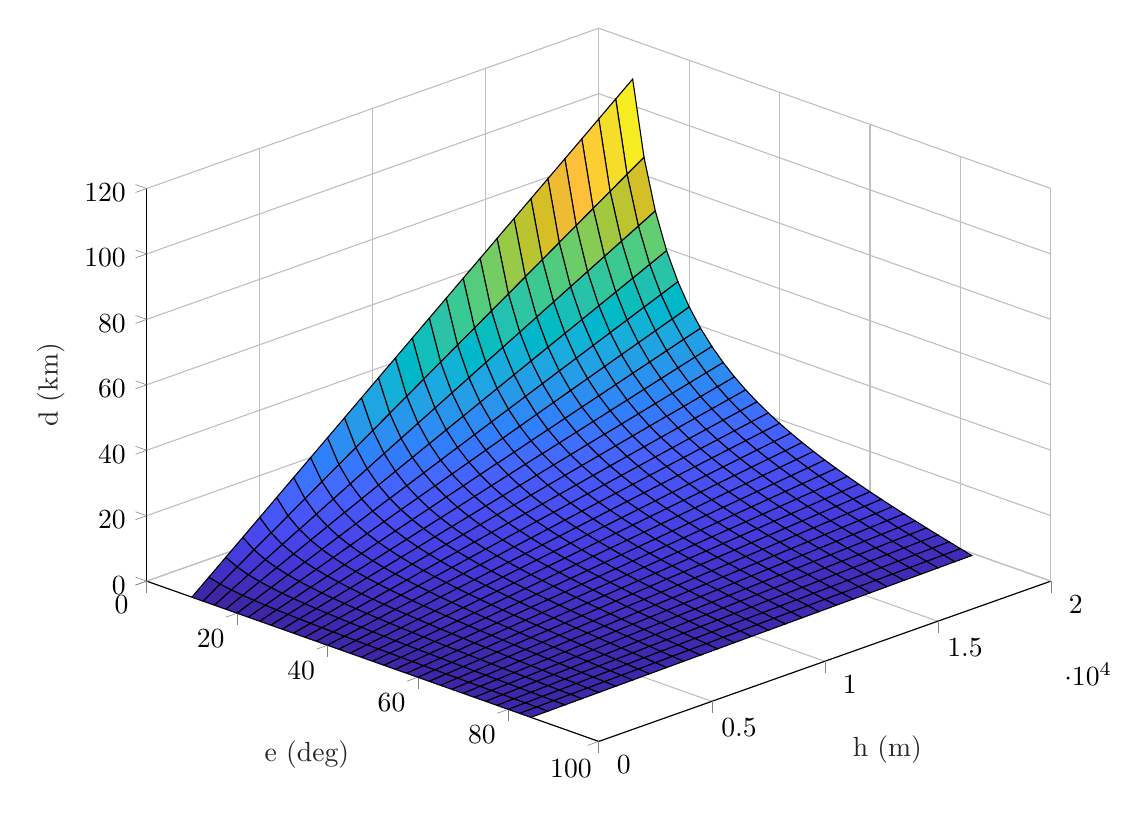
\begin{tikzpicture}

\begin{axis}[%
width=4.521in,
height=3.566in,
at={(0.758in,0.481in)},
scale only axis,
xmin=0,
xmax=100,
tick align=outside,
xlabel style={font=\color{white!15!black}},
xlabel={e (deg)},
ymin=0,
ymax=20000,
ylabel style={font=\color{white!15!black}},
ylabel={h (m)},
zmin=0,
zmax=120,
zlabel style={font=\color{white!15!black}},
zlabel={d (km)},
view={45}{30},
axis background/.style={fill=white},
axis x line*=bottom,
axis y line*=left,
axis z line*=left,
xmajorgrids,
ymajorgrids,
zmajorgrids
]

\addplot3[%
surf,
shader=flat corner, draw=black, z buffer=sort, colormap={mymap}{[1pt] rgb(0pt)=(0.2422,0.1504,0.6603); rgb(1pt)=(0.2444,0.1534,0.6728); rgb(2pt)=(0.2464,0.1569,0.6847); rgb(3pt)=(0.2484,0.1607,0.6961); rgb(4pt)=(0.2503,0.1648,0.7071); rgb(5pt)=(0.2522,0.1689,0.7179); rgb(6pt)=(0.254,0.1732,0.7286); rgb(7pt)=(0.2558,0.1773,0.7393); rgb(8pt)=(0.2576,0.1814,0.7501); rgb(9pt)=(0.2594,0.1854,0.761); rgb(11pt)=(0.2628,0.1932,0.7828); rgb(12pt)=(0.2645,0.1972,0.7937); rgb(13pt)=(0.2661,0.2011,0.8043); rgb(14pt)=(0.2676,0.2052,0.8148); rgb(15pt)=(0.2691,0.2094,0.8249); rgb(16pt)=(0.2704,0.2138,0.8346); rgb(17pt)=(0.2717,0.2184,0.8439); rgb(18pt)=(0.2729,0.2231,0.8528); rgb(19pt)=(0.274,0.228,0.8612); rgb(20pt)=(0.2749,0.233,0.8692); rgb(21pt)=(0.2758,0.2382,0.8767); rgb(22pt)=(0.2766,0.2435,0.884); rgb(23pt)=(0.2774,0.2489,0.8908); rgb(24pt)=(0.2781,0.2543,0.8973); rgb(25pt)=(0.2788,0.2598,0.9035); rgb(26pt)=(0.2794,0.2653,0.9094); rgb(27pt)=(0.2798,0.2708,0.915); rgb(28pt)=(0.2802,0.2764,0.9204); rgb(29pt)=(0.2806,0.2819,0.9255); rgb(30pt)=(0.2809,0.2875,0.9305); rgb(31pt)=(0.2811,0.293,0.9352); rgb(32pt)=(0.2813,0.2985,0.9397); rgb(33pt)=(0.2814,0.304,0.9441); rgb(34pt)=(0.2814,0.3095,0.9483); rgb(35pt)=(0.2813,0.315,0.9524); rgb(36pt)=(0.2811,0.3204,0.9563); rgb(37pt)=(0.2809,0.3259,0.96); rgb(38pt)=(0.2807,0.3313,0.9636); rgb(39pt)=(0.2803,0.3367,0.967); rgb(40pt)=(0.2798,0.3421,0.9702); rgb(41pt)=(0.2791,0.3475,0.9733); rgb(42pt)=(0.2784,0.3529,0.9763); rgb(43pt)=(0.2776,0.3583,0.9791); rgb(44pt)=(0.2766,0.3638,0.9817); rgb(45pt)=(0.2754,0.3693,0.984); rgb(46pt)=(0.2741,0.3748,0.9862); rgb(47pt)=(0.2726,0.3804,0.9881); rgb(48pt)=(0.271,0.386,0.9898); rgb(49pt)=(0.2691,0.3916,0.9912); rgb(50pt)=(0.267,0.3973,0.9924); rgb(51pt)=(0.2647,0.403,0.9935); rgb(52pt)=(0.2621,0.4088,0.9946); rgb(53pt)=(0.2591,0.4145,0.9955); rgb(54pt)=(0.2556,0.4203,0.9965); rgb(55pt)=(0.2517,0.4261,0.9974); rgb(56pt)=(0.2473,0.4319,0.9983); rgb(57pt)=(0.2424,0.4378,0.9991); rgb(58pt)=(0.2369,0.4437,0.9996); rgb(59pt)=(0.2311,0.4497,0.9995); rgb(60pt)=(0.225,0.4559,0.9985); rgb(61pt)=(0.2189,0.462,0.9968); rgb(62pt)=(0.2128,0.4682,0.9948); rgb(63pt)=(0.2066,0.4743,0.9926); rgb(64pt)=(0.2006,0.4803,0.9906); rgb(65pt)=(0.195,0.4861,0.9887); rgb(66pt)=(0.1903,0.4919,0.9867); rgb(67pt)=(0.1869,0.4975,0.9844); rgb(68pt)=(0.1847,0.503,0.9819); rgb(69pt)=(0.1831,0.5084,0.9793); rgb(70pt)=(0.1818,0.5138,0.9766); rgb(71pt)=(0.1806,0.5191,0.9738); rgb(72pt)=(0.1795,0.5244,0.9709); rgb(73pt)=(0.1785,0.5296,0.9677); rgb(74pt)=(0.1778,0.5349,0.9641); rgb(75pt)=(0.1773,0.5401,0.9602); rgb(76pt)=(0.1768,0.5452,0.956); rgb(77pt)=(0.1764,0.5504,0.9516); rgb(78pt)=(0.1755,0.5554,0.9473); rgb(79pt)=(0.174,0.5605,0.9432); rgb(80pt)=(0.1716,0.5655,0.9393); rgb(81pt)=(0.1686,0.5705,0.9357); rgb(82pt)=(0.1649,0.5755,0.9323); rgb(83pt)=(0.161,0.5805,0.9289); rgb(84pt)=(0.1573,0.5854,0.9254); rgb(85pt)=(0.154,0.5902,0.9218); rgb(86pt)=(0.1513,0.595,0.9182); rgb(87pt)=(0.1492,0.5997,0.9147); rgb(88pt)=(0.1475,0.6043,0.9113); rgb(89pt)=(0.1461,0.6089,0.908); rgb(90pt)=(0.1446,0.6135,0.905); rgb(91pt)=(0.1429,0.618,0.9022); rgb(92pt)=(0.1408,0.6226,0.8998); rgb(93pt)=(0.1383,0.6272,0.8975); rgb(94pt)=(0.1354,0.6317,0.8953); rgb(95pt)=(0.1321,0.6363,0.8932); rgb(96pt)=(0.1288,0.6408,0.891); rgb(97pt)=(0.1253,0.6453,0.8887); rgb(98pt)=(0.1219,0.6497,0.8862); rgb(99pt)=(0.1185,0.6541,0.8834); rgb(100pt)=(0.1152,0.6584,0.8804); rgb(101pt)=(0.1119,0.6627,0.877); rgb(102pt)=(0.1085,0.6669,0.8734); rgb(103pt)=(0.1048,0.671,0.8695); rgb(104pt)=(0.1009,0.675,0.8653); rgb(105pt)=(0.0964,0.6789,0.8609); rgb(106pt)=(0.0914,0.6828,0.8562); rgb(107pt)=(0.0855,0.6865,0.8513); rgb(108pt)=(0.0789,0.6902,0.8462); rgb(109pt)=(0.0713,0.6938,0.8409); rgb(110pt)=(0.0628,0.6972,0.8355); rgb(111pt)=(0.0535,0.7006,0.8299); rgb(112pt)=(0.0433,0.7039,0.8242); rgb(113pt)=(0.0328,0.7071,0.8183); rgb(114pt)=(0.0234,0.7103,0.8124); rgb(115pt)=(0.0155,0.7133,0.8064); rgb(116pt)=(0.0091,0.7163,0.8003); rgb(117pt)=(0.0046,0.7192,0.7941); rgb(118pt)=(0.0019,0.722,0.7878); rgb(119pt)=(0.0009,0.7248,0.7815); rgb(120pt)=(0.0018,0.7275,0.7752); rgb(121pt)=(0.0046,0.7301,0.7688); rgb(122pt)=(0.0094,0.7327,0.7623); rgb(123pt)=(0.0162,0.7352,0.7558); rgb(124pt)=(0.0253,0.7376,0.7492); rgb(125pt)=(0.0369,0.74,0.7426); rgb(126pt)=(0.0504,0.7423,0.7359); rgb(127pt)=(0.0638,0.7446,0.7292); rgb(128pt)=(0.077,0.7468,0.7224); rgb(129pt)=(0.0899,0.7489,0.7156); rgb(130pt)=(0.1023,0.751,0.7088); rgb(131pt)=(0.1141,0.7531,0.7019); rgb(132pt)=(0.1252,0.7552,0.695); rgb(133pt)=(0.1354,0.7572,0.6881); rgb(134pt)=(0.1448,0.7593,0.6812); rgb(135pt)=(0.1532,0.7614,0.6741); rgb(136pt)=(0.1609,0.7635,0.6671); rgb(137pt)=(0.1678,0.7656,0.6599); rgb(138pt)=(0.1741,0.7678,0.6527); rgb(139pt)=(0.1799,0.7699,0.6454); rgb(140pt)=(0.1853,0.7721,0.6379); rgb(141pt)=(0.1905,0.7743,0.6303); rgb(142pt)=(0.1954,0.7765,0.6225); rgb(143pt)=(0.2003,0.7787,0.6146); rgb(144pt)=(0.2061,0.7808,0.6065); rgb(145pt)=(0.2118,0.7828,0.5983); rgb(146pt)=(0.2178,0.7849,0.5899); rgb(147pt)=(0.2244,0.7869,0.5813); rgb(148pt)=(0.2318,0.7887,0.5725); rgb(149pt)=(0.2401,0.7905,0.5636); rgb(150pt)=(0.2491,0.7922,0.5546); rgb(151pt)=(0.2589,0.7937,0.5454); rgb(152pt)=(0.2695,0.7951,0.536); rgb(153pt)=(0.2809,0.7964,0.5266); rgb(154pt)=(0.2929,0.7975,0.517); rgb(155pt)=(0.3052,0.7985,0.5074); rgb(156pt)=(0.3176,0.7994,0.4975); rgb(157pt)=(0.3301,0.8002,0.4876); rgb(158pt)=(0.3424,0.8009,0.4774); rgb(159pt)=(0.3548,0.8016,0.4669); rgb(160pt)=(0.3671,0.8021,0.4563); rgb(161pt)=(0.3795,0.8026,0.4454); rgb(162pt)=(0.3921,0.8029,0.4344); rgb(163pt)=(0.405,0.8031,0.4233); rgb(164pt)=(0.4184,0.803,0.4122); rgb(165pt)=(0.4322,0.8028,0.4013); rgb(166pt)=(0.4463,0.8024,0.3904); rgb(167pt)=(0.4608,0.8018,0.3797); rgb(168pt)=(0.4753,0.8011,0.3691); rgb(169pt)=(0.4899,0.8002,0.3586); rgb(170pt)=(0.5044,0.7993,0.348); rgb(171pt)=(0.5187,0.7982,0.3374); rgb(172pt)=(0.5329,0.797,0.3267); rgb(173pt)=(0.547,0.7957,0.3159); rgb(175pt)=(0.5748,0.7929,0.2941); rgb(176pt)=(0.5886,0.7913,0.2833); rgb(177pt)=(0.6024,0.7896,0.2726); rgb(178pt)=(0.6161,0.7878,0.2622); rgb(179pt)=(0.6297,0.7859,0.2521); rgb(180pt)=(0.6433,0.7839,0.2423); rgb(181pt)=(0.6567,0.7818,0.2329); rgb(182pt)=(0.6701,0.7796,0.2239); rgb(183pt)=(0.6833,0.7773,0.2155); rgb(184pt)=(0.6963,0.775,0.2075); rgb(185pt)=(0.7091,0.7727,0.1998); rgb(186pt)=(0.7218,0.7703,0.1924); rgb(187pt)=(0.7344,0.7679,0.1852); rgb(188pt)=(0.7468,0.7654,0.1782); rgb(189pt)=(0.759,0.7629,0.1717); rgb(190pt)=(0.771,0.7604,0.1658); rgb(191pt)=(0.7829,0.7579,0.1608); rgb(192pt)=(0.7945,0.7554,0.157); rgb(193pt)=(0.806,0.7529,0.1546); rgb(194pt)=(0.8172,0.7505,0.1535); rgb(195pt)=(0.8281,0.7481,0.1536); rgb(196pt)=(0.8389,0.7457,0.1546); rgb(197pt)=(0.8495,0.7435,0.1564); rgb(198pt)=(0.86,0.7413,0.1587); rgb(199pt)=(0.8703,0.7392,0.1615); rgb(200pt)=(0.8804,0.7372,0.165); rgb(201pt)=(0.8903,0.7353,0.1695); rgb(202pt)=(0.9,0.7336,0.1749); rgb(203pt)=(0.9093,0.7321,0.1815); rgb(204pt)=(0.9184,0.7308,0.189); rgb(205pt)=(0.9272,0.7298,0.1973); rgb(206pt)=(0.9357,0.729,0.2061); rgb(207pt)=(0.944,0.7285,0.2151); rgb(208pt)=(0.9523,0.7284,0.2237); rgb(209pt)=(0.9606,0.7285,0.2312); rgb(210pt)=(0.9689,0.7292,0.2373); rgb(211pt)=(0.977,0.7304,0.2418); rgb(212pt)=(0.9842,0.733,0.2446); rgb(213pt)=(0.99,0.7365,0.2429); rgb(214pt)=(0.9946,0.7407,0.2394); rgb(215pt)=(0.9966,0.7458,0.2351); rgb(216pt)=(0.9971,0.7513,0.2309); rgb(217pt)=(0.9972,0.7569,0.2267); rgb(218pt)=(0.9971,0.7626,0.2224); rgb(219pt)=(0.9969,0.7683,0.2181); rgb(220pt)=(0.9966,0.774,0.2138); rgb(221pt)=(0.9962,0.7798,0.2095); rgb(222pt)=(0.9957,0.7856,0.2053); rgb(223pt)=(0.9949,0.7915,0.2012); rgb(224pt)=(0.9938,0.7974,0.1974); rgb(225pt)=(0.9923,0.8034,0.1939); rgb(226pt)=(0.9906,0.8095,0.1906); rgb(227pt)=(0.9885,0.8156,0.1875); rgb(228pt)=(0.9861,0.8218,0.1846); rgb(229pt)=(0.9835,0.828,0.1817); rgb(230pt)=(0.9807,0.8342,0.1787); rgb(231pt)=(0.9778,0.8404,0.1757); rgb(232pt)=(0.9748,0.8467,0.1726); rgb(233pt)=(0.972,0.8529,0.1695); rgb(234pt)=(0.9694,0.8591,0.1665); rgb(235pt)=(0.9671,0.8654,0.1636); rgb(236pt)=(0.9651,0.8716,0.1608); rgb(237pt)=(0.9634,0.8778,0.1582); rgb(238pt)=(0.9619,0.884,0.1557); rgb(239pt)=(0.9608,0.8902,0.1532); rgb(240pt)=(0.9601,0.8963,0.1507); rgb(241pt)=(0.9596,0.9023,0.148); rgb(242pt)=(0.9595,0.9084,0.145); rgb(243pt)=(0.9597,0.9143,0.1418); rgb(244pt)=(0.9601,0.9203,0.1382); rgb(245pt)=(0.9608,0.9262,0.1344); rgb(246pt)=(0.9618,0.932,0.1304); rgb(247pt)=(0.9629,0.9379,0.1261); rgb(248pt)=(0.9642,0.9437,0.1216); rgb(249pt)=(0.9657,0.9494,0.1168); rgb(250pt)=(0.9674,0.9552,0.1116); rgb(251pt)=(0.9692,0.9609,0.1061); rgb(252pt)=(0.9711,0.9667,0.1001); rgb(253pt)=(0.973,0.9724,0.0938); rgb(254pt)=(0.9749,0.9782,0.0872); rgb(255pt)=(0.9769,0.9839,0.0805)}, mesh/rows=27]
table[row sep=crcr, point meta=\thisrow{c}] {%
%
x	y	z	c\\
10	0	0	0\\
12.5	0	0	0\\
15	0	0	0\\
17.5	0	0	0\\
20	0	0	0\\
22.5	0	0	0\\
25	0	0	0\\
27.5	0	0	0\\
30	0	0	0\\
32.5	0	0	0\\
35	0	0	0\\
37.5	0	0	0\\
40	0	0	0\\
42.5	0	0	0\\
45	0	0	0\\
47.5	0	0	0\\
50	0	0	0\\
52.5	0	0	0\\
55	0	0	0\\
57.5	0	0	0\\
60	0	0	0\\
62.5	0	0	0\\
65	0	0	0\\
67.5	0	0	0\\
70	0	0	0\\
72.5	0	0	0\\
75	0	0	0\\
77.5	0	0	0\\
80	0	0	0\\
82.5	0	0	0\\
85	0	0	0\\
10	750	4.25346136471328	4.25346136471328\\
12.5	750	3.38303137774654	3.38303137774654\\
15	750	2.79903810567666	2.79903810567666\\
17.5	750	2.37869610177241	2.37869610177241\\
20	750	2.06060806459097	2.06060806459097\\
22.5	750	1.81066017177982	1.81066017177982\\
25	750	1.60838019038217	1.60838019038217\\
27.5	750	1.44073659522837	1.44073659522837\\
30	750	1.29903810567666	1.29903810567666\\
32.5	750	1.17726418283812	1.17726418283812\\
35	750	1.07111100505659	1.07111100505659\\
37.5	750	0.977419029630904	0.977419029630904\\
40	750	0.893815194445657	0.893815194445657\\
42.5	750	0.818481375801953	0.818481375801953\\
45	750	0.75	0.75\\
47.5	750	0.687248380513068	0.687248380513068\\
50	750	0.62932472338296	0.62932472338296\\
52.5	750	0.57549524098422	0.57549524098422\\
55	750	0.525155653657282	0.525155653657282\\
57.5	750	0.47780269560562	0.47780269560562\\
60	750	0.433012701892219	0.433012701892219\\
62.5	750	0.39042528791381	0.39042528791381\\
65	750	0.349730743616249	0.349730743616249\\
67.5	750	0.310660171779821	0.310660171779821\\
70	750	0.272977675699652	0.272977675699652\\
72.5	750	0.236474091659238	0.236474091659238\\
75	750	0.200961894323342	0.200961894323342\\
77.5	750	0.166270996982205	0.166270996982205\\
80	750	0.132245235531349	0.132245235531349\\
82.5	750	0.0987393731905469	0.0987393731905469\\
85	750	0.065616497644443	0.065616497644443\\
10	1500	8.50692272942656	8.50692272942656\\
12.5	1500	6.76606275549308	6.76606275549308\\
15	1500	5.59807621135332	5.59807621135332\\
17.5	1500	4.75739220354482	4.75739220354482\\
20	1500	4.12121612918193	4.12121612918193\\
22.5	1500	3.62132034355964	3.62132034355964\\
25	1500	3.21676038076434	3.21676038076434\\
27.5	1500	2.88147319045675	2.88147319045675\\
30	1500	2.59807621135332	2.59807621135332\\
32.5	1500	2.35452836567624	2.35452836567624\\
35	1500	2.14222201011317	2.14222201011317\\
37.5	1500	1.95483805926181	1.95483805926181\\
40	1500	1.78763038889131	1.78763038889131\\
42.5	1500	1.63696275160391	1.63696275160391\\
45	1500	1.5	1.5\\
47.5	1500	1.37449676102614	1.37449676102614\\
50	1500	1.25864944676592	1.25864944676592\\
52.5	1500	1.15099048196844	1.15099048196844\\
55	1500	1.05031130731456	1.05031130731456\\
57.5	1500	0.95560539121124	0.95560539121124\\
60	1500	0.866025403784439	0.866025403784439\\
62.5	1500	0.780850575827619	0.780850575827619\\
65	1500	0.699461487232498	0.699461487232498\\
67.5	1500	0.621320343559643	0.621320343559643\\
70	1500	0.545955351399304	0.545955351399304\\
72.5	1500	0.472948183318475	0.472948183318475\\
75	1500	0.401923788646684	0.401923788646684\\
77.5	1500	0.33254199396441	0.33254199396441\\
80	1500	0.264490471062697	0.264490471062697\\
82.5	1500	0.197478746381094	0.197478746381094\\
85	1500	0.131232995288886	0.131232995288886\\
10	2250	12.7603840941398	12.7603840941398\\
12.5	2250	10.1490941332396	10.1490941332396\\
15	2250	8.39711431702997	8.39711431702997\\
17.5	2250	7.13608830531723	7.13608830531723\\
20	2250	6.1818241937729	6.1818241937729\\
22.5	2250	5.43198051533946	5.43198051533946\\
25	2250	4.82514057114651	4.82514057114651\\
27.5	2250	4.32220978568512	4.32220978568512\\
30	2250	3.89711431702997	3.89711431702997\\
32.5	2250	3.53179254851435	3.53179254851435\\
35	2250	3.21333301516976	3.21333301516976\\
37.5	2250	2.93225708889271	2.93225708889271\\
40	2250	2.68144558333697	2.68144558333697\\
42.5	2250	2.45544412740586	2.45544412740586\\
45	2250	2.25	2.25\\
47.5	2250	2.0617451415392	2.0617451415392\\
50	2250	1.88797417014888	1.88797417014888\\
52.5	2250	1.72648572295266	1.72648572295266\\
55	2250	1.57546696097185	1.57546696097185\\
57.5	2250	1.43340808681686	1.43340808681686\\
60	2250	1.29903810567666	1.29903810567666\\
62.5	2250	1.17127586374143	1.17127586374143\\
65	2250	1.04919223084875	1.04919223084875\\
67.5	2250	0.931980515339464	0.931980515339464\\
70	2250	0.818933027098955	0.818933027098955\\
72.5	2250	0.709422274977713	0.709422274977713\\
75	2250	0.602885682970026	0.602885682970026\\
77.5	2250	0.498812990946615	0.498812990946615\\
80	2250	0.396735706594046	0.396735706594046\\
82.5	2250	0.296218119571641	0.296218119571641\\
85	2250	0.196849492933329	0.196849492933329\\
10	3000	17.0138454588531	17.0138454588531\\
12.5	3000	13.5321255109862	13.5321255109862\\
15	3000	11.1961524227066	11.1961524227066\\
17.5	3000	9.51478440708964	9.51478440708964\\
20	3000	8.24243225836387	8.24243225836387\\
22.5	3000	7.24264068711929	7.24264068711929\\
25	3000	6.43352076152868	6.43352076152868\\
27.5	3000	5.7629463809135	5.7629463809135\\
30	3000	5.19615242270663	5.19615242270663\\
32.5	3000	4.70905673135247	4.70905673135247\\
35	3000	4.28444402022634	4.28444402022634\\
37.5	3000	3.90967611852362	3.90967611852362\\
40	3000	3.57526077778263	3.57526077778263\\
42.5	3000	3.27392550320781	3.27392550320781\\
45	3000	3	3\\
47.5	3000	2.74899352205227	2.74899352205227\\
50	3000	2.51729889353184	2.51729889353184\\
52.5	3000	2.30198096393688	2.30198096393688\\
55	3000	2.10062261462913	2.10062261462913\\
57.5	3000	1.91121078242248	1.91121078242248\\
60	3000	1.73205080756888	1.73205080756888\\
62.5	3000	1.56170115165524	1.56170115165524\\
65	3000	1.398922974465	1.398922974465\\
67.5	3000	1.24264068711929	1.24264068711929\\
70	3000	1.09191070279861	1.09191070279861\\
72.5	3000	0.945896366636951	0.945896366636951\\
75	3000	0.803847577293368	0.803847577293368\\
77.5	3000	0.66508398792882	0.66508398792882\\
80	3000	0.528980942125395	0.528980942125395\\
82.5	3000	0.394957492762188	0.394957492762188\\
85	3000	0.262465990577772	0.262465990577772\\
10	3750	21.2673068235664	21.2673068235664\\
12.5	3750	16.9151568887327	16.9151568887327\\
15	3750	13.9951905283833	13.9951905283833\\
17.5	3750	11.893480508862	11.893480508862\\
20	3750	10.3030403229548	10.3030403229548\\
22.5	3750	9.05330085889911	9.05330085889911\\
25	3750	8.04190095191085	8.04190095191085\\
27.5	3750	7.20368297614187	7.20368297614187\\
30	3750	6.49519052838329	6.49519052838329\\
32.5	3750	5.88632091419059	5.88632091419059\\
35	3750	5.35555502528293	5.35555502528293\\
37.5	3750	4.88709514815452	4.88709514815452\\
40	3750	4.46907597222829	4.46907597222829\\
42.5	3750	4.09240687900977	4.09240687900977\\
45	3750	3.75	3.75\\
47.5	3750	3.43624190256534	3.43624190256534\\
50	3750	3.1466236169148	3.1466236169148\\
52.5	3750	2.8774762049211	2.8774762049211\\
55	3750	2.62577826828641	2.62577826828641\\
57.5	3750	2.3890134780281	2.3890134780281\\
60	3750	2.1650635094611	2.1650635094611\\
62.5	3750	1.95212643956905	1.95212643956905\\
65	3750	1.74865371808124	1.74865371808124\\
67.5	3750	1.55330085889911	1.55330085889911\\
70	3750	1.36488837849826	1.36488837849826\\
72.5	3750	1.18237045829619	1.18237045829619\\
75	3750	1.00480947161671	1.00480947161671\\
77.5	3750	0.831354984911025	0.831354984911025\\
80	3750	0.661226177656744	0.661226177656744\\
82.5	3750	0.493696865952734	0.493696865952734\\
85	3750	0.328082488222215	0.328082488222215\\
10	4500	25.5207681882797	25.5207681882797\\
12.5	4500	20.2981882664793	20.2981882664793\\
15	4500	16.7942286340599	16.7942286340599\\
17.5	4500	14.2721766106345	14.2721766106345\\
20	4500	12.3636483875458	12.3636483875458\\
22.5	4500	10.8639610306789	10.8639610306789\\
25	4500	9.65028114229301	9.65028114229301\\
27.5	4500	8.64441957137024	8.64441957137024\\
30	4500	7.79422863405995	7.79422863405995\\
32.5	4500	7.06358509702871	7.06358509702871\\
35	4500	6.42666603033952	6.42666603033952\\
37.5	4500	5.86451417778543	5.86451417778543\\
40	4500	5.36289116667395	5.36289116667395\\
42.5	4500	4.91088825481172	4.91088825481172\\
45	4500	4.5	4.5\\
47.5	4500	4.12349028307841	4.12349028307841\\
50	4500	3.77594834029776	3.77594834029776\\
52.5	4500	3.45297144590532	3.45297144590532\\
55	4500	3.15093392194369	3.15093392194369\\
57.5	4500	2.86681617363372	2.86681617363372\\
60	4500	2.59807621135332	2.59807621135332\\
62.5	4500	2.34255172748286	2.34255172748286\\
65	4500	2.09838446169749	2.09838446169749\\
67.5	4500	1.86396103067893	1.86396103067893\\
70	4500	1.63786605419791	1.63786605419791\\
72.5	4500	1.41884454995543	1.41884454995543\\
75	4500	1.20577136594005	1.20577136594005\\
77.5	4500	0.99762598189323	0.99762598189323\\
80	4500	0.793471413188092	0.793471413188092\\
82.5	4500	0.592436239143281	0.592436239143281\\
85	4500	0.393698985866658	0.393698985866658\\
10	5250	29.774229552993	29.774229552993\\
12.5	5250	23.6812196442258	23.6812196442258\\
15	5250	19.5932667397366	19.5932667397366\\
17.5	5250	16.6508727124069	16.6508727124069\\
20	5250	14.4242564521368	14.4242564521368\\
22.5	5250	12.6746212024587	12.6746212024587\\
25	5250	11.2586613326752	11.2586613326752\\
27.5	5250	10.0851561665986	10.0851561665986\\
30	5250	9.09326673973661	9.09326673973661\\
32.5	5250	8.24084927986683	8.24084927986683\\
35	5250	7.4977770353961	7.4977770353961\\
37.5	5250	6.84193320741633	6.84193320741633\\
40	5250	6.2567063611196	6.2567063611196\\
42.5	5250	5.72936963061367	5.72936963061367\\
45	5250	5.25	5.25\\
47.5	5250	4.81073866359147	4.81073866359147\\
50	5250	4.40527306368072	4.40527306368072\\
52.5	5250	4.02846668688954	4.02846668688954\\
55	5250	3.67608957560098	3.67608957560098\\
57.5	5250	3.34461886923934	3.34461886923934\\
60	5250	3.03108891324554	3.03108891324554\\
62.5	5250	2.73297701539667	2.73297701539667\\
65	5250	2.44811520531374	2.44811520531374\\
67.5	5250	2.17462120245875	2.17462120245875\\
70	5250	1.91084372989756	1.91084372989756\\
72.5	5250	1.65531864161466	1.65531864161466\\
75	5250	1.40673326026339	1.40673326026339\\
77.5	5250	1.16389697887543	1.16389697887543\\
80	5250	0.925716648719441	0.925716648719441\\
82.5	5250	0.691175612333828	0.691175612333828\\
85	5250	0.459315483511101	0.459315483511101\\
10	6000	34.0276909177063	34.0276909177063\\
12.5	6000	27.0642510219723	27.0642510219723\\
15	6000	22.3923048454133	22.3923048454133\\
17.5	6000	19.0295688141793	19.0295688141793\\
20	6000	16.4848645167277	16.4848645167277\\
22.5	6000	14.4852813742386	14.4852813742386\\
25	6000	12.8670415230574	12.8670415230574\\
27.5	6000	11.525892761827	11.525892761827\\
30	6000	10.3923048454133	10.3923048454133\\
32.5	6000	9.41811346270494	9.41811346270494\\
35	6000	8.56888804045269	8.56888804045269\\
37.5	6000	7.81935223704723	7.81935223704723\\
40	6000	7.15052155556526	7.15052155556526\\
42.5	6000	6.54785100641563	6.54785100641563\\
45	6000	6	6\\
47.5	6000	5.49798704410454	5.49798704410454\\
50	6000	5.03459778706368	5.03459778706368\\
52.5	6000	4.60396192787376	4.60396192787376\\
55	6000	4.20124522925826	4.20124522925826\\
57.5	6000	3.82242156484496	3.82242156484496\\
60	6000	3.46410161513775	3.46410161513775\\
62.5	6000	3.12340230331048	3.12340230331048\\
65	6000	2.79784594892999	2.79784594892999\\
67.5	6000	2.48528137423857	2.48528137423857\\
70	6000	2.18382140559721	2.18382140559721\\
72.5	6000	1.8917927332739	1.8917927332739\\
75	6000	1.60769515458674	1.60769515458674\\
77.5	6000	1.33016797585764	1.33016797585764\\
80	6000	1.05796188425079	1.05796188425079\\
82.5	6000	0.789914985524375	0.789914985524375\\
85	6000	0.524931981155544	0.524931981155544\\
10	6750	38.2811522824195	38.2811522824195\\
12.5	6750	30.4472823997189	30.4472823997189\\
15	6750	25.1913429510899	25.1913429510899\\
17.5	6750	21.4082649159517	21.4082649159517\\
20	6750	18.5454725813187	18.5454725813187\\
22.5	6750	16.2959415460184	16.2959415460184\\
25	6750	14.4754217134395	14.4754217134395\\
27.5	6750	12.9666293570554	12.9666293570554\\
30	6750	11.6913429510899	11.6913429510899\\
32.5	6750	10.5953776455431	10.5953776455431\\
35	6750	9.63999904550927	9.63999904550927\\
37.5	6750	8.79677126667814	8.79677126667814\\
40	6750	8.04433675001092	8.04433675001092\\
42.5	6750	7.36633238221758	7.36633238221758\\
45	6750	6.75	6.75\\
47.5	6750	6.18523542461761	6.18523542461761\\
50	6750	5.66392251044664	5.66392251044664\\
52.5	6750	5.17945716885798	5.17945716885798\\
55	6750	4.72640088291554	4.72640088291554\\
57.5	6750	4.30022426045058	4.30022426045058\\
60	6750	3.89711431702997	3.89711431702997\\
62.5	6750	3.51382759122429	3.51382759122429\\
65	6750	3.14757669254624	3.14757669254624\\
67.5	6750	2.79594154601839	2.79594154601839\\
70	6750	2.45679908129687	2.45679908129687\\
72.5	6750	2.12826682493314	2.12826682493314\\
75	6750	1.80865704891008	1.80865704891008\\
77.5	6750	1.49643897283984	1.49643897283984\\
80	6750	1.19020711978214	1.19020711978214\\
82.5	6750	0.888654358714922	0.888654358714922\\
85	6750	0.590548478799987	0.590548478799987\\
10	7500	42.5346136471328	42.5346136471328\\
12.5	7500	33.8303137774654	33.8303137774654\\
15	7500	27.9903810567666	27.9903810567666\\
17.5	7500	23.7869610177241	23.7869610177241\\
20	7500	20.6060806459097	20.6060806459097\\
22.5	7500	18.1066017177982	18.1066017177982\\
25	7500	16.0838019038217	16.0838019038217\\
27.5	7500	14.4073659522837	14.4073659522837\\
30	7500	12.9903810567666	12.9903810567666\\
32.5	7500	11.7726418283812	11.7726418283812\\
35	7500	10.7111100505659	10.7111100505659\\
37.5	7500	9.77419029630904	9.77419029630904\\
40	7500	8.93815194445657	8.93815194445657\\
42.5	7500	8.18481375801953	8.18481375801953\\
45	7500	7.5	7.5\\
47.5	7500	6.87248380513068	6.87248380513068\\
50	7500	6.2932472338296	6.2932472338296\\
52.5	7500	5.7549524098422	5.7549524098422\\
55	7500	5.25155653657282	5.25155653657282\\
57.5	7500	4.7780269560562	4.7780269560562\\
60	7500	4.33012701892219	4.33012701892219\\
62.5	7500	3.9042528791381	3.9042528791381\\
65	7500	3.49730743616249	3.49730743616249\\
67.5	7500	3.10660171779821	3.10660171779821\\
70	7500	2.72977675699652	2.72977675699652\\
72.5	7500	2.36474091659238	2.36474091659238\\
75	7500	2.00961894323342	2.00961894323342\\
77.5	7500	1.66270996982205	1.66270996982205\\
80	7500	1.32245235531349	1.32245235531349\\
82.5	7500	0.987393731905469	0.987393731905469\\
85	7500	0.65616497644443	0.65616497644443\\
10	8250	46.7880750118461	46.7880750118461\\
12.5	8250	37.213345155212	37.213345155212\\
15	8250	30.7894191624432	30.7894191624432\\
17.5	8250	26.1656571194965	26.1656571194965\\
20	8250	22.6666887105006	22.6666887105006\\
22.5	8250	19.917261889578	19.917261889578\\
25	8250	17.6921820942039	17.6921820942039\\
27.5	8250	15.8481025475121	15.8481025475121\\
30	8250	14.2894191624432	14.2894191624432\\
32.5	8250	12.9499060112193	12.9499060112193\\
35	8250	11.7822210556224	11.7822210556224\\
37.5	8250	10.7516093259399	10.7516093259399\\
40	8250	9.83196713890223	9.83196713890223\\
42.5	8250	9.00329513382149	9.00329513382149\\
45	8250	8.25	8.25\\
47.5	8250	7.55973218564374	7.55973218564374\\
50	8250	6.92257195721256	6.92257195721256\\
52.5	8250	6.33044765082642	6.33044765082642\\
55	8250	5.77671219023011	5.77671219023011\\
57.5	8250	5.25582965166182	5.25582965166182\\
60	8250	4.76313972081441	4.76313972081441\\
62.5	8250	4.29467816705191	4.29467816705191\\
65	8250	3.84703817977874	3.84703817977874\\
67.5	8250	3.41726188957803	3.41726188957803\\
70	8250	3.00275443269617	3.00275443269617\\
72.5	8250	2.60121500825161	2.60121500825161\\
75	8250	2.21058083755676	2.21058083755676\\
77.5	8250	1.82898096680425	1.82898096680425\\
80	8250	1.45469759084484	1.45469759084484\\
82.5	8250	1.08613310509602	1.08613310509602\\
85	8250	0.721781474088873	0.721781474088873\\
10	9000	51.0415363765594	51.0415363765594\\
12.5	9000	40.5963765329585	40.5963765329585\\
15	9000	33.5884572681199	33.5884572681199\\
17.5	9000	28.5443532212689	28.5443532212689\\
20	9000	24.7272967750916	24.7272967750916\\
22.5	9000	21.7279220613579	21.7279220613579\\
25	9000	19.300562284586	19.300562284586\\
27.5	9000	17.2888391427405	17.2888391427405\\
30	9000	15.5884572681199	15.5884572681199\\
32.5	9000	14.1271701940574	14.1271701940574\\
35	9000	12.853332060679	12.853332060679\\
37.5	9000	11.7290283555709	11.7290283555709\\
40	9000	10.7257823333479	10.7257823333479\\
42.5	9000	9.82177650962344	9.82177650962344\\
45	9000	9	9\\
47.5	9000	8.24698056615681	8.24698056615681\\
50	9000	7.55189668059552	7.55189668059552\\
52.5	9000	6.90594289181064	6.90594289181064\\
55	9000	6.30186784388739	6.30186784388739\\
57.5	9000	5.73363234726744	5.73363234726744\\
60	9000	5.19615242270663	5.19615242270663\\
62.5	9000	4.68510345496572	4.68510345496572\\
65	9000	4.19676892339499	4.19676892339499\\
67.5	9000	3.72792206135786	3.72792206135786\\
70	9000	3.27573210839582	3.27573210839582\\
72.5	9000	2.83768909991085	2.83768909991085\\
75	9000	2.4115427318801	2.4115427318801\\
77.5	9000	1.99525196378646	1.99525196378646\\
80	9000	1.58694282637618	1.58694282637618\\
82.5	9000	1.18487247828656	1.18487247828656\\
85	9000	0.787397971733316	0.787397971733316\\
10	9750	55.2949977412727	55.2949977412727\\
12.5	9750	43.9794079107051	43.9794079107051\\
15	9750	36.3874953737966	36.3874953737966\\
17.5	9750	30.9230493230413	30.9230493230413\\
20	9750	26.7879048396826	26.7879048396826\\
22.5	9750	23.5385822331377	23.5385822331377\\
25	9750	20.9089424749682	20.9089424749682\\
27.5	9750	18.7295757379689	18.7295757379689\\
30	9750	16.8874953737966	16.8874953737966\\
32.5	9750	15.3044343768955	15.3044343768955\\
35	9750	13.9244430657356	13.9244430657356\\
37.5	9750	12.7064473852018	12.7064473852018\\
40	9750	11.6195975277935	11.6195975277935\\
42.5	9750	10.6402578854254	10.6402578854254\\
45	9750	9.75	9.75\\
47.5	9750	8.93422894666988	8.93422894666988\\
50	9750	8.18122140397848	8.18122140397848\\
52.5	9750	7.48143813279486	7.48143813279486\\
55	9750	6.82702349754467	6.82702349754467\\
57.5	9750	6.21143504287306	6.21143504287306\\
60	9750	5.62916512459885	5.62916512459885\\
62.5	9750	5.07552874287953	5.07552874287953\\
65	9750	4.54649966701124	4.54649966701124\\
67.5	9750	4.03858223313768	4.03858223313768\\
70	9750	3.54870978409547	3.54870978409547\\
72.5	9750	3.07416319157009	3.07416319157009\\
75	9750	2.61250462620345	2.61250462620345\\
77.5	9750	2.16152296076866	2.16152296076866\\
80	9750	1.71918806190753	1.71918806190753\\
82.5	9750	1.28361185147711	1.28361185147711\\
85	9750	0.853014469377759	0.853014469377759\\
10	10500	59.548459105986	59.548459105986\\
12.5	10500	47.3624392884516	47.3624392884516\\
15	10500	39.1865334794732	39.1865334794732\\
17.5	10500	33.3017454248137	33.3017454248137\\
20	10500	28.8485129042735	28.8485129042735\\
22.5	10500	25.3492424049175	25.3492424049175\\
25	10500	22.5173226653504	22.5173226653504\\
27.5	10500	20.1703123331972	20.1703123331972\\
30	10500	18.1865334794732	18.1865334794732\\
32.5	10500	16.4816985597337	16.4816985597337\\
35	10500	14.9955540707922	14.9955540707922\\
37.5	10500	13.6838664148327	13.6838664148327\\
40	10500	12.5134127222392	12.5134127222392\\
42.5	10500	11.4587392612273	11.4587392612273\\
45	10500	10.5	10.5\\
47.5	10500	9.62147732718295	9.62147732718295\\
50	10500	8.81054612736144	8.81054612736144\\
52.5	10500	8.05693337377908	8.05693337377908\\
55	10500	7.35217915120195	7.35217915120195\\
57.5	10500	6.68923773847868	6.68923773847868\\
60	10500	6.06217782649107	6.06217782649107\\
62.5	10500	5.46595403079334	5.46595403079334\\
65	10500	4.89623041062748	4.89623041062748\\
67.5	10500	4.3492424049175	4.3492424049175\\
70	10500	3.82168745979512	3.82168745979512\\
72.5	10500	3.31063728322933	3.31063728322933\\
75	10500	2.81346652052679	2.81346652052679\\
77.5	10500	2.32779395775087	2.32779395775087\\
80	10500	1.85143329743888	1.85143329743888\\
82.5	10500	1.38235122466766	1.38235122466766\\
85	10500	0.918630967022202	0.918630967022202\\
10	11250	63.8019204706992	63.8019204706992\\
12.5	11250	50.7454706661981	50.7454706661981\\
15	11250	41.9855715851499	41.9855715851499\\
17.5	11250	35.6804415265861	35.6804415265861\\
20	11250	30.9091209688645	30.9091209688645\\
22.5	11250	27.1599025766973	27.1599025766973\\
25	11250	24.1257028557325	24.1257028557325\\
27.5	11250	21.6110489284256	21.6110489284256\\
30	11250	19.4855715851499	19.4855715851499\\
32.5	11250	17.6589627425718	17.6589627425718\\
35	11250	16.0666650758488	16.0666650758488\\
37.5	11250	14.6612854444636	14.6612854444636\\
40	11250	13.4072279166849	13.4072279166849\\
42.5	11250	12.2772206370293	12.2772206370293\\
45	11250	11.25	11.25\\
47.5	11250	10.308725707696	10.308725707696\\
50	11250	9.4398708507444	9.4398708507444\\
52.5	11250	8.6324286147633	8.6324286147633\\
55	11250	7.87733480485923	7.87733480485923\\
57.5	11250	7.1670404340843	7.1670404340843\\
60	11250	6.49519052838329	6.49519052838329\\
62.5	11250	5.85637931870715	5.85637931870715\\
65	11250	5.24596115424373	5.24596115424373\\
67.5	11250	4.65990257669732	4.65990257669732\\
70	11250	4.09466513549478	4.09466513549478\\
72.5	11250	3.54711137488856	3.54711137488856\\
75	11250	3.01442841485013	3.01442841485013\\
77.5	11250	2.49406495473307	2.49406495473307\\
80	11250	1.98367853297023	1.98367853297023\\
82.5	11250	1.4810905978582	1.4810905978582\\
85	11250	0.984247464666645	0.984247464666645\\
10	12000	68.0553818354125	68.0553818354125\\
12.5	12000	54.1285020439447	54.1285020439447\\
15	12000	44.7846096908265	44.7846096908265\\
17.5	12000	38.0591376283586	38.0591376283586\\
20	12000	32.9697290334555	32.9697290334555\\
22.5	12000	28.9705627484771	28.9705627484771\\
25	12000	25.7340830461147	25.7340830461147\\
27.5	12000	23.051785523654	23.051785523654\\
30	12000	20.7846096908265	20.7846096908265\\
32.5	12000	18.8362269254099	18.8362269254099\\
35	12000	17.1377760809054	17.1377760809054\\
37.5	12000	15.6387044740945	15.6387044740945\\
40	12000	14.3010431111305	14.3010431111305\\
42.5	12000	13.0957020128313	13.0957020128313\\
45	12000	12	12\\
47.5	12000	10.9959740882091	10.9959740882091\\
50	12000	10.0691955741274	10.0691955741274\\
52.5	12000	9.20792385574752	9.20792385574752\\
55	12000	8.40249045851652	8.40249045851652\\
57.5	12000	7.64484312968992	7.64484312968992\\
60	12000	6.92820323027551	6.92820323027551\\
62.5	12000	6.24680460662096	6.24680460662096\\
65	12000	5.59569189785998	5.59569189785998\\
67.5	12000	4.97056274847714	4.97056274847714\\
70	12000	4.36764281119443	4.36764281119443\\
72.5	12000	3.7835854665478	3.7835854665478\\
75	12000	3.21539030917347	3.21539030917347\\
77.5	12000	2.66033595171528	2.66033595171528\\
80	12000	2.11592376850158	2.11592376850158\\
82.5	12000	1.57982997104875	1.57982997104875\\
85	12000	1.04986396231109	1.04986396231109\\
10	12750	72.3088432001258	72.3088432001258\\
12.5	12750	57.5115334216912	57.5115334216912\\
15	12750	47.5836477965032	47.5836477965032\\
17.5	12750	40.437833730131	40.437833730131\\
20	12750	35.0303370980464	35.0303370980464\\
22.5	12750	30.781222920257	30.781222920257\\
25	12750	27.3424632364969	27.3424632364969\\
27.5	12750	24.4925221188824	24.4925221188824\\
30	12750	22.0836477965032	22.0836477965032\\
32.5	12750	20.013491108248	20.013491108248\\
35	12750	18.208887085962	18.208887085962\\
37.5	12750	16.6161235037254	16.6161235037254\\
40	12750	15.1948583055762	15.1948583055762\\
42.5	12750	13.9141833886332	13.9141833886332\\
45	12750	12.75	12.75\\
47.5	12750	11.6832224687221	11.6832224687221\\
50	12750	10.6985202975103	10.6985202975103\\
52.5	12750	9.78341909673174	9.78341909673174\\
55	12750	8.9276461121738	8.9276461121738\\
57.5	12750	8.12264582529554	8.12264582529554\\
60	12750	7.36121593216773	7.36121593216773\\
62.5	12750	6.63722989453477	6.63722989453477\\
65	12750	5.94542264147623	5.94542264147623\\
67.5	12750	5.28122292025696	5.28122292025696\\
70	12750	4.64062048689408	4.64062048689408\\
72.5	12750	4.02005955820704	4.02005955820704\\
75	12750	3.41635220349681	3.41635220349681\\
77.5	12750	2.82660694869748	2.82660694869748\\
80	12750	2.24816900403293	2.24816900403293\\
82.5	12750	1.6785693442393	1.6785693442393\\
85	12750	1.11548045995553	1.11548045995553\\
10	13500	76.5623045648391	76.5623045648391\\
12.5	13500	60.8945647994378	60.8945647994378\\
15	13500	50.3826859021798	50.3826859021798\\
17.5	13500	42.8165298319034	42.8165298319034\\
20	13500	37.0909451626374	37.0909451626374\\
22.5	13500	32.5918830920368	32.5918830920368\\
25	13500	28.950843426879	28.950843426879\\
27.5	13500	25.9332587141107	25.9332587141107\\
30	13500	23.3826859021798	23.3826859021798\\
32.5	13500	21.1907552910861	21.1907552910861\\
35	13500	19.2799980910185	19.2799980910185\\
37.5	13500	17.5935425333563	17.5935425333563\\
40	13500	16.0886735000218	16.0886735000218\\
42.5	13500	14.7326647644352	14.7326647644352\\
45	13500	13.5	13.5\\
47.5	13500	12.3704708492352	12.3704708492352\\
50	13500	11.3278450208933	11.3278450208933\\
52.5	13500	10.358914337716	10.358914337716\\
55	13500	9.45280176583108	9.45280176583108\\
57.5	13500	8.60044852090116	8.60044852090116\\
60	13500	7.79422863405995	7.79422863405995\\
62.5	13500	7.02765518244857	7.02765518244857\\
65	13500	6.29515338509248	6.29515338509248\\
67.5	13500	5.59188309203678	5.59188309203678\\
70	13500	4.91359816259373	4.91359816259373\\
72.5	13500	4.25653364986628	4.25653364986628\\
75	13500	3.61731409782016	3.61731409782016\\
77.5	13500	2.99287794567969	2.99287794567969\\
80	13500	2.38041423956428	2.38041423956428\\
82.5	13500	1.77730871742984	1.77730871742984\\
85	13500	1.18109695759997	1.18109695759997\\
10	14250	80.8157659295524	80.8157659295524\\
12.5	14250	64.2775961771843	64.2775961771843\\
15	14250	53.1817240078565	53.1817240078565\\
17.5	14250	45.1952259336758	45.1952259336758\\
20	14250	39.1515532272284	39.1515532272284\\
22.5	14250	34.4025432638166	34.4025432638166\\
25	14250	30.5592236172612	30.5592236172612\\
27.5	14250	27.3739953093391	27.3739953093391\\
30	14250	24.6817240078565	24.6817240078565\\
32.5	14250	22.3680194739242	22.3680194739242\\
35	14250	20.3511090960751	20.3511090960751\\
37.5	14250	18.5709615629872	18.5709615629872\\
40	14250	16.9824886944675	16.9824886944675\\
42.5	14250	15.5511461402371	15.5511461402371\\
45	14250	14.25	14.25\\
47.5	14250	13.0577192297483	13.0577192297483\\
50	14250	11.9571697442762	11.9571697442762\\
52.5	14250	10.9344095787002	10.9344095787002\\
55	14250	9.97795741948836	9.97795741948836\\
57.5	14250	9.07825121650678	9.07825121650678\\
60	14250	8.22724133595217	8.22724133595217\\
62.5	14250	7.41808047036239	7.41808047036239\\
65	14250	6.64488412870873	6.64488412870873\\
67.5	14250	5.9025432638166	5.9025432638166\\
70	14250	5.18657583829338	5.18657583829338\\
72.5	14250	4.49300774152552	4.49300774152552\\
75	14250	3.8182759921435	3.8182759921435\\
77.5	14250	3.15914894266189	3.15914894266189\\
80	14250	2.51265947509563	2.51265947509563\\
82.5	14250	1.87604809062039	1.87604809062039\\
85	14250	1.24671345524442	1.24671345524442\\
10	15000	85.0692272942656	85.0692272942656\\
12.5	15000	67.6606275549309	67.6606275549309\\
15	15000	55.9807621135332	55.9807621135332\\
17.5	15000	47.5739220354482	47.5739220354482\\
20	15000	41.2121612918193	41.2121612918193\\
22.5	15000	36.2132034355964	36.2132034355964\\
25	15000	32.1676038076434	32.1676038076434\\
27.5	15000	28.8147319045675	28.8147319045675\\
30	15000	25.9807621135332	25.9807621135332\\
32.5	15000	23.5452836567624	23.5452836567624\\
35	15000	21.4222201011317	21.4222201011317\\
37.5	15000	19.5483805926181	19.5483805926181\\
40	15000	17.8763038889131	17.8763038889131\\
42.5	15000	16.3696275160391	16.3696275160391\\
45	15000	15	15\\
47.5	15000	13.7449676102614	13.7449676102614\\
50	15000	12.5864944676592	12.5864944676592\\
52.5	15000	11.5099048196844	11.5099048196844\\
55	15000	10.5031130731456	10.5031130731456\\
57.5	15000	9.5560539121124	9.5560539121124\\
60	15000	8.66025403784439	8.66025403784439\\
62.5	15000	7.80850575827619	7.80850575827619\\
65	15000	6.99461487232498	6.99461487232498\\
67.5	15000	6.21320343559643	6.21320343559643\\
70	15000	5.45955351399304	5.45955351399304\\
72.5	15000	4.72948183318475	4.72948183318475\\
75	15000	4.01923788646684	4.01923788646684\\
77.5	15000	3.3254199396441	3.3254199396441\\
80	15000	2.64490471062697	2.64490471062697\\
82.5	15000	1.97478746381094	1.97478746381094\\
85	15000	1.31232995288886	1.31232995288886\\
10	15750	89.3226886589789	89.3226886589789\\
12.5	15750	71.0436589326774	71.0436589326774\\
15	15750	58.7798002192098	58.7798002192098\\
17.5	15750	49.9526181372206	49.9526181372206\\
20	15750	43.2727693564103	43.2727693564103\\
22.5	15750	38.0238636073762	38.0238636073762\\
25	15750	33.7759839980256	33.7759839980256\\
27.5	15750	30.2554684997959	30.2554684997959\\
30	15750	27.2798002192098	27.2798002192098\\
32.5	15750	24.7225478396005	24.7225478396005\\
35	15750	22.4933311061883	22.4933311061883\\
37.5	15750	20.525799622249	20.525799622249\\
40	15750	18.7701190833588	18.7701190833588\\
42.5	15750	17.188108891841	17.188108891841\\
45	15750	15.75	15.75\\
47.5	15750	14.4322159907744	14.4322159907744\\
50	15750	13.2158191910422	13.2158191910422\\
52.5	15750	12.0854000606686	12.0854000606686\\
55	15750	11.0282687268029	11.0282687268029\\
57.5	15750	10.033856607718	10.033856607718\\
60	15750	9.09326673973661	9.09326673973661\\
62.5	15750	8.19893104619	8.19893104619\\
65	15750	7.34434561594123	7.34434561594123\\
67.5	15750	6.52386360737625	6.52386360737625\\
70	15750	5.73253118969269	5.73253118969269\\
72.5	15750	4.96595592484399	4.96595592484399\\
75	15750	4.22019978079018	4.22019978079018\\
77.5	15750	3.4916909366263	3.4916909366263\\
80	15750	2.77714994615832	2.77714994615832\\
82.5	15750	2.07352683700148	2.07352683700148\\
85	15750	1.3779464505333	1.3779464505333\\
10	16500	93.5761500236922	93.5761500236922\\
12.5	16500	74.426690310424	74.426690310424\\
15	16500	61.5788383248865	61.5788383248865\\
17.5	16500	52.331314238993	52.331314238993\\
20	16500	45.3333774210013	45.3333774210013\\
22.5	16500	39.8345237791561	39.8345237791561\\
25	16500	35.3843641884077	35.3843641884077\\
27.5	16500	31.6962050950242	31.6962050950242\\
30	16500	28.5788383248865	28.5788383248865\\
32.5	16500	25.8998120224386	25.8998120224386\\
35	16500	23.5644421112449	23.5644421112449\\
37.5	16500	21.5032186518799	21.5032186518799\\
40	16500	19.6639342778045	19.6639342778045\\
42.5	16500	18.006590267643	18.006590267643\\
45	16500	16.5	16.5\\
47.5	16500	15.1194643712875	15.1194643712875\\
50	16500	13.8451439144251	13.8451439144251\\
52.5	16500	12.6608953016528	12.6608953016528\\
55	16500	11.5534243804602	11.5534243804602\\
57.5	16500	10.5116593033236	10.5116593033236\\
60	16500	9.52627944162882	9.52627944162882\\
62.5	16500	8.58935633410381	8.58935633410381\\
65	16500	7.69407635955748	7.69407635955748\\
67.5	16500	6.83452377915607	6.83452377915607\\
70	16500	6.00550886539234	6.00550886539234\\
72.5	16500	5.20243001650323	5.20243001650323\\
75	16500	4.42116167511352	4.42116167511352\\
77.5	16500	3.65796193360851	3.65796193360851\\
80	16500	2.90939518168967	2.90939518168967\\
82.5	16500	2.17226621019203	2.17226621019203\\
85	16500	1.44356294817775	1.44356294817775\\
10	17250	97.8296113884055	97.8296113884055\\
12.5	17250	77.8097216881705	77.8097216881705\\
15	17250	64.3778764305631	64.3778764305631\\
17.5	17250	54.7100103407654	54.7100103407654\\
20	17250	47.3939854855922	47.3939854855922\\
22.5	17250	41.6451839509359	41.6451839509359\\
25	17250	36.9927443787899	36.9927443787899\\
27.5	17250	33.1369416902526	33.1369416902526\\
30	17250	29.8778764305631	29.8778764305631\\
32.5	17250	27.0770762052767	27.0770762052767\\
35	17250	24.6355531163015	24.6355531163015\\
37.5	17250	22.4806376815108	22.4806376815108\\
40	17250	20.5577494722501	20.5577494722501\\
42.5	17250	18.8250716434449	18.8250716434449\\
45	17250	17.25	17.25\\
47.5	17250	15.8067127518006	15.8067127518006\\
50	17250	14.4744686378081	14.4744686378081\\
52.5	17250	13.2363905426371	13.2363905426371\\
55	17250	12.0785800341175	12.0785800341175\\
57.5	17250	10.9894619989293	10.9894619989293\\
60	17250	9.95929214352105	9.95929214352105\\
62.5	17250	8.97978162201762	8.97978162201762\\
65	17250	8.04380710317372	8.04380710317372\\
67.5	17250	7.14518395093589	7.14518395093589\\
70	17250	6.27848654109199	6.27848654109199\\
72.5	17250	5.43890410816247	5.43890410816247\\
75	17250	4.62212356943687	4.62212356943687\\
77.5	17250	3.82423293059071	3.82423293059071\\
80	17250	3.04164041722102	3.04164041722102\\
82.5	17250	2.27100558338258	2.27100558338258\\
85	17250	1.50917944582219	1.50917944582219\\
10	18000	102.083072753119	102.083072753119\\
12.5	18000	81.192753065917	81.192753065917\\
15	18000	67.1769145362398	67.1769145362398\\
17.5	18000	57.0887064425378	57.0887064425378\\
20	18000	49.4545935501832	49.4545935501832\\
22.5	18000	43.4558441227157	43.4558441227157\\
25	18000	38.6011245691721	38.6011245691721\\
27.5	18000	34.577678285481	34.577678285481\\
30	18000	31.1769145362398	31.1769145362398\\
32.5	18000	28.2543403881148	28.2543403881148\\
35	18000	25.7066641213581	25.7066641213581\\
37.5	18000	23.4580567111417	23.4580567111417\\
40	18000	21.4515646666958	21.4515646666958\\
42.5	18000	19.6435530192469	19.6435530192469\\
45	18000	18	18\\
47.5	18000	16.4939611323136	16.4939611323136\\
50	18000	15.103793361191	15.103793361191\\
52.5	18000	13.8118857836213	13.8118857836213\\
55	18000	12.6037356877748	12.6037356877748\\
57.5	18000	11.4672646945349	11.4672646945349\\
60	18000	10.3923048454133	10.3923048454133\\
62.5	18000	9.37020690993143	9.37020690993143\\
65	18000	8.39353784678998	8.39353784678998\\
67.5	18000	7.45584412271571	7.45584412271571\\
70	18000	6.55146421679164	6.55146421679164\\
72.5	18000	5.6753781998217	5.6753781998217\\
75	18000	4.82308546376021	4.82308546376021\\
77.5	18000	3.99050392757292	3.99050392757292\\
80	18000	3.17388565275237	3.17388565275237\\
82.5	18000	2.36974495657313	2.36974495657313\\
85	18000	1.57479594346663	1.57479594346663\\
10	18750	106.336534117832	106.336534117832\\
12.5	18750	84.5757844436636	84.5757844436636\\
15	18750	69.9759526419165	69.9759526419165\\
17.5	18750	59.4674025443102	59.4674025443102\\
20	18750	51.5152016147742	51.5152016147742\\
22.5	18750	45.2665042944955	45.2665042944955\\
25	18750	40.2095047595542	40.2095047595542\\
27.5	18750	36.0184148807094	36.0184148807094\\
30	18750	32.4759526419165	32.4759526419165\\
32.5	18750	29.4316045709529	29.4316045709529\\
35	18750	26.7777751264146	26.7777751264146\\
37.5	18750	24.4354757407726	24.4354757407726\\
40	18750	22.3453798611414	22.3453798611414\\
42.5	18750	20.4620343950488	20.4620343950488\\
45	18750	18.75	18.75\\
47.5	18750	17.1812095128267	17.1812095128267\\
50	18750	15.733118084574	15.733118084574\\
52.5	18750	14.3873810246055	14.3873810246055\\
55	18750	13.1288913414321	13.1288913414321\\
57.5	18750	11.9450673901405	11.9450673901405\\
60	18750	10.8253175473055	10.8253175473055\\
62.5	18750	9.76063219784524	9.76063219784524\\
65	18750	8.74326859040622	8.74326859040622\\
67.5	18750	7.76650429449553	7.76650429449553\\
70	18750	6.82444189249129	6.82444189249129\\
72.5	18750	5.91185229148094	5.91185229148094\\
75	18750	5.02404735808355	5.02404735808355\\
77.5	18750	4.15677492455512	4.15677492455512\\
80	18750	3.30613088828372	3.30613088828372\\
82.5	18750	2.46848432976367	2.46848432976367\\
85	18750	1.64041244111108	1.64041244111108\\
10	19500	110.589995482545	110.589995482545\\
12.5	19500	87.9588158214101	87.9588158214101\\
15	19500	72.7749907475931	72.7749907475931\\
17.5	19500	61.8460986460826	61.8460986460826\\
20	19500	53.5758096793651	53.5758096793651\\
22.5	19500	47.0771644662754	47.0771644662754\\
25	19500	41.8178849499364	41.8178849499364\\
27.5	19500	37.4591514759377	37.4591514759377\\
30	19500	33.7749907475931	33.7749907475931\\
32.5	19500	30.6088687537911	30.6088687537911\\
35	19500	27.8488861314712	27.8488861314712\\
37.5	19500	25.4128947704035	25.4128947704035\\
40	19500	23.2391950555871	23.2391950555871\\
42.5	19500	21.2805157708508	21.2805157708508\\
45	19500	19.5	19.5\\
47.5	19500	17.8684578933398	17.8684578933398\\
50	19500	16.362442807957	16.362442807957\\
52.5	19500	14.9628762655897	14.9628762655897\\
55	19500	13.6540469950893	13.6540469950893\\
57.5	19500	12.4228700857461	12.4228700857461\\
60	19500	11.2583302491977	11.2583302491977\\
62.5	19500	10.1510574857591	10.1510574857591\\
65	19500	9.09299933402247	9.09299933402247\\
67.5	19500	8.07716446627535	8.07716446627535\\
70	19500	7.09741956819095	7.09741956819095\\
72.5	19500	6.14832638314018	6.14832638314018\\
75	19500	5.22500925240689	5.22500925240689\\
77.5	19500	4.32304592153733	4.32304592153733\\
80	19500	3.43837612381507	3.43837612381507\\
82.5	19500	2.56722370295422	2.56722370295422\\
85	19500	1.70602893875552	1.70602893875552\\
};
\end{axis}
\end{tikzpicture}%
  \caption{Interception range ($d$) as a function of minimum elevation angle ($e$) and operational altitude of the eavesdropper ($h$).}
  \label{fig-interception-range}
\end{figure}

%\noindent
Figure \ref{fig-interception-range} shows the interception range $d_{Eve}$ in the range $e_{Alice} = [10^\circ, 85^\circ], h_{Eve} = [100,20000]$.
In the resulting 3D plot, the dependent variable or the interception range ($d_{Eve}$) of the airborne eavesdropper is on the vertical axis.
Independent variables or the minimum elevation angle of the terminal ($e_{Alice}$) and opertional altitude of the airborne eavesdropper ($h_{Eve}$) are on the horizontal axes.

The convex surface exhebits linear growth in relation to altitude $h_{Eve}$ and accelerating tangential growth in relation to $e_{Alice}$.
Therefore, we can deduce that the minimum elevation angle is in most cases the driving factor of the maximum interception range of a VSAT ground station.
The influence of $h_{Eve}$ on $d_{Eve}$ is markedly smaller but still significant, especially when considering terminals with small $e_{Alice}$.
The tangent function has asymptotes at $e_{Alice} = \pi / 2 + n\pi$. Within the given limits, the asymptotes are not reached and the resulting surface is smooth and continuous.

%% TODO: Takaisin reaalimaailmaan alamallin osalta

\subsection{Submodel 2: Beam tracking potential}

\begin{figure}[h]
  \centering
  \usetikzlibrary{calc,3d,intersections, positioning,shapes}

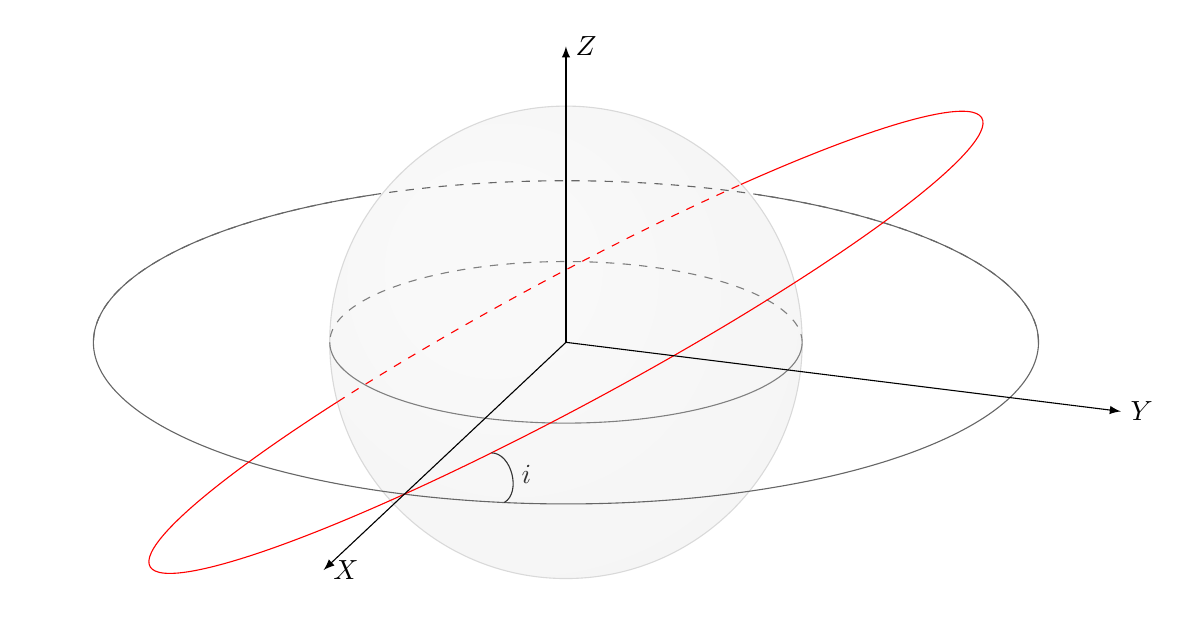
\begin{tikzpicture}[scale=2]
  \pgfmathsetmacro{\Re}{1.5}
  \pgfmathsetmacro{\Ro}{3} 
  \fill[ball color=white!10, opacity=0.025] (0,0,0) circle ({\Re}); % 3D lighting effect
  \tdplotsetmaincoords{70}{110}
  \begin{scope}[tdplot_main_coords, shift={(0,0)}]
    \coordinate (O) at (0,0,0); % origin

    % ball perimeter, gray
    \pgfmathsetmacro{\thetavec}{70}
    \pgfmathsetmacro{\phivec}{20}
    \tdplotsetrotatedcoords{\phivec}{\thetavec}{0}
    \tdplotdrawarc[tdplot_rotated_coords,color=gray!30]{(O)}{\Re}{0}{360}{}{}

    % equator
    \pgfmathsetmacro{\thetavec}{0}
    \pgfmathsetmacro{\phivec}{0}
    \tdplotsetrotatedcoords{\phivec}{\thetavec}{0}
    \tdplotdrawarc[tdplot_rotated_coords,color=black!50]{(O)}{\Re}{-70}{110}{}{}
    \tdplotdrawarc[tdplot_rotated_coords,color=black!50, dashed]{(O)}{\Re}{110}{290}{}{}
    %\node[] at (-1,2,1) {\textcolor{blue}{\scriptsize $\alpha=\thetavec \, ,  \, $\beta=\phivec}};

    % equatorial orbit
    \pgfmathsetmacro{\thetavec}{0}
    \pgfmathsetmacro{\phivec}{0}
    \tdplotsetrotatedcoords{\phivec}{\thetavec}{0}
    \tdplotdrawarc[tdplot_rotated_coords,color=black!60]{(O)}{3}{-136}{176}{}{}
    \tdplotdrawarc[tdplot_rotated_coords,color=black!60, dashed]{(O)}{3}{110}{290}{}{}

    % inclined orbit
    \pgfmathsetmacro{\i}{-30}
    \pgfmathsetmacro{\p}{90}
    \pgfmathsetmacro{\thetavec}{\i}
    \pgfmathsetmacro{\phivec}{\p}
    \tdplotsetrotatedcoords{\phivec}{\thetavec}{0}
    \tdplotdrawarc[tdplot_rotated_coords,color=red]{(O)}{3}{-214}{88}{}{}
    \tdplotdrawarc[tdplot_rotated_coords,color=red, dashed]{(O)}{3}{360-214}{88}{}{}

    % inclination
    \pgfmathsetmacro{\alpha}{12.5}
    \path ({\Ro * cos(\alpha)},{\Ro * sin(\alpha)},{0}) coordinate (I1);
    \path[tdplot_rotated_coords] ({\Ro * cos(-(\alpha - \p))},
      {\Ro * sin(-(\alpha + \p))},{0}) coordinate (I2);
    \draw[color=black!80] (I1) to[out=390,in=0] node[pos=0.5,right] {$i$} (I2);

    %axis
    \coordinate (X) at (4.5,0,0) ;
    \coordinate (Y) at (0,3.75,0) ;
    \coordinate (Z) at (0,0,2) ;

    \draw[-latex] (O) -- (X) node[anchor=west] {$X$};
    \draw[-latex] (O) -- (Y) node[anchor=west] {$Y$};
    \draw[-latex] (O) -- (Z) node[anchor=west] {$Z$};

  \end{scope}
  
\end{tikzpicture}

  \caption{Geometry of a circular Earth orbit.}
  \label{fig-orbit-geometry}
\end{figure}

In addition to being aligned along the line-of-sight of the VSAT's main lobe, the eavesdropper needs to be able to intercept sufficiently long transmission to be able to %ilmaista lähettäjän olemus. 
This time dimension brings another point to consider when evaluating the risk of eavesdropping.
Different durations of interception have varying implications for the legitimate transmitter.
As an practical example, // millisecond-level? // signal capture might be enough for DF applications, while COMINT would require the eavesdropper to intercept the data stream from minutes to days type of durations.

Maximum duration of signal interception is set by the ability of the airborne platform to track the main lobe of the earth station.
The beam movement is primarily driven by the motion of the receiving satellite in orbit, which is in turn governed by Kepler's laws of orbital motion.
Tracking capability of the aircraft can be evaluated by analysing the velocity of the sub-satellite point at the eavesdropper's operational altitude (point x on figure \ref{fig-orbit-geometry}).
If this velocity exceeds the cruise speed of the eavesdropper, the airborne platform is not able to continuously follow the uplink RF beam, which limits the time window into individual satellite passes.

\subsubsection{Equatorial orbits}

Communication satellites reside often in circular orbits, which are a special case when evaluating Kepler's laws of orbital motion.
Here, the velocity of the sub-satellite point can be computed by solving Kepler's third law for the orbital velocity at a set altitude.
In equatorial orbits, Earth's rotation can be directly substracted from the angular velocity of the satellite, as both share roughly the same rotational axis.

\begin{equation} \label{eq-kepler-3}
  T^2 = (\frac{4\pi^2}{GM})r^3
\end{equation}

where $T$ is the orbital period, $G$ is the gravitational constant, $M$ is the mass of the orbited body and $r$ is the radius of the orbit %measured from the centre of mass of the orbited body.

In essence, the aircraft can be modeled as a low-flying athmospheric satellite.
This allows for the same equations to be used in modeling its kinematic characteristics.
Solving the required velocity for successful beam tracking can be computed by equating the required orbital period of the aircraft to the one of the space-borne satellite.

Orbital period is related to the angular velocity of the satellite $\omega_{sat}$ through the equation

\begin{equation} \label{eq-ang-vel-1}
  \omega_{sat} = \frac{2\pi}{T}
\end{equation}

\noindent
which can be used to solve the tangential velocity component at a set altitude $v_r$

\begin{equation} \label{eq-ang-vel-2}
  v_r = \omega r
\end{equation}

\noindent
As $\omega_{sat} = \omega_{air}$ in the case that the aircraft is able to continuosly track the satellite, the velocity of the sub-satellite point at the cruising altitude of the aircraft $v_{r, air}$ can be solved by combining equations (\ref{eq-kepler-3}), (\ref{eq-ang-vel-1}) and (\ref{eq-ang-vel-2}).
Rearranging Kepler's third law to solve for $v_{r, air}$ gives

\begin{equation} \label{eq-v-air-equatorial}
  v_{r, air} = r_{air} \sqrt{\frac{G M_E}{r_{sat}^3}}
\end{equation}

\noindent
Variables $r_{air}$ and $r_{sat}$ are the orbital radiuses of the eavesdropping aircraft and the receiving satellite measured from the center of the Earth while $M_E$ is the mass of the Earth.
Equation (\ref{eq-v-air-equatorial}) gives $v_{r, air}$ in the ECI coordinate frame.
To compute the actual movement of the sub-satellite point relative to the surface of the Earth, the velocity figure needs to be converted to the ECF coordinate system.
For circular equatorial orbits, this can be simply achieved by substracting the spin of the Earth from $v_{r, air}$.

\begin{equation}
  v_{r, ECF} = v_{r, air} - \omega_E r_{air}
\end{equation}

\noindent
$\omega_E$ is the angular velocity of the Earth at the equator.

\begin{figure}[h]
  \centering
  % This file was created by matlab2tikz.
%
%The latest updates can be retrieved from
%  http://www.mathworks.com/matlabcentral/fileexchange/22022-matlab2tikz-matlab2tikz
%where you can also make suggestions and rate matlab2tikz.
%
\definecolor{mycolor1}{rgb}{0.00000,0.44700,0.74100}%
%
\begin{tikzpicture}

\begin{axis}[%
width=4.521in,
height=3.566in,
at={(0.758in,0.481in)},
scale only axis,
xmin=0,
xmax=40000000,
ymin=0,
ymax=8000,
axis background/.style={fill=white}
]
\addplot [color=mycolor1, forget plot]
  table[row sep=crcr]{%
500000	7072.71764129545\\
1000000	6365.41441116611\\
1500000	5768.61401343729\\
2000000	5259.57169914256\\
2500000	4821.22680484161\\
3000000	4440.55812330651\\
3500000	4107.47348810996\\
4000000	3814.04289796006\\
4500000	3553.95812701838\\
5000000	3322.14500116304\\
5500000	3114.480651329\\
6000000	2927.58426192998\\
6500000	2758.66012043392\\
7000000	2605.37844395658\\
7500000	2465.78386645891\\
8000000	2338.22443445674\\
8500000	2221.29598506997\\
9000000	2113.7981854881\\
9500000	2014.69950110221\\
10000000	1923.10906331822\\
10500000	1838.25391523213\\
11000000	1759.46048288005\\
11500000	1686.13939180947\\
12000000	1617.77295091573\\
12500000	1553.90477714283\\
13000000	1494.13114936631\\
13500000	1438.093767251\\
14000000	1385.47365808604\\
14500000	1335.98602660745\\
15000000	1289.37588333773\\
15500000	1245.41431874345\\
16000000	1203.89531557571\\
16500000	1164.63301164729\\
17000000	1127.45934116856\\
17500000	1092.22199549238\\
18000000	1058.7826543787\\
18500000	1027.01544720074\\
19000000	996.805610277406\\
19500000	968.048312044218\\
20000000	940.647622311633\\
20500000	914.515605598319\\
21000000	889.57152161971\\
21500000	865.741118580401\\
22000000	842.956007059067\\
22500000	821.153104064185\\
23000000	800.274138340326\\
23500000	780.265209268467\\
24000000	761.076392770707\\
24500000	742.661388533194\\
25000000	724.977203628275\\
25500000	707.983868270195\\
26000000	691.644179996502\\
26500000	675.923473044846\\
27000000	660.789410104709\\
27500000	646.211793976132\\
28000000	632.162396971571\\
28500000	618.614806159755\\
29000000	605.544282778029\\
29500000	592.927634337247\\
30000000	580.743098115126\\
30500000	568.970234883794\\
31000000	557.589831848052\\
31500000	546.583813885374\\
32000000	535.935162279006\\
32500000	525.627840223627\\
33000000	515.646724460593\\
33500000	505.97754246809\\
34000000	496.606814691834\\
34500000	487.521801355257\\
35000000	478.710453435377\\
35500000	470.161367432379\\
36000000	461.863743598168\\
36500000	453.807347322214\\
37000000	445.982473402509\\
};
\end{axis}
\end{tikzpicture}%
  \caption{Sub-satellite velocity as a function of orbital altitude (m) in equatiorial orbits.}
  \label{fig-subsat-velocity-equatiorial}
\end{figure}

Figure \ref{fig-subsat-velocity-equatiorial} shows the sub-satellite velocity ($v_{r, air}$) of a satellite in equatorial orbit as a function of orbital height $h_{sat} = r_{sat} - R_{E}$, where $R_{E}$ is the radius of the Earth.
Velocities are examined in orbits ranging from LEO to GEO, which corresponds to the range $h_{sat} = [5 \cdot 10^5, 3.7 \cdot 10^7]$.
In the resulting graph, the dependent variable or the sub-satellite velocity ($v_{r, air}$) is on the vertical axis, while the independent variable of the orbital height $h_{sat}$ is on the horizontal axis.
The graph can be observed approaching the rotational velocity of the Earth when $h_{sat}$ approaches the height of GEO 36000 km.
As the graph is computed in the ECF coordinate frame, we can se sub-satellite velocity approaching zero, which means that the satellite appears fixed in its position in the sky.
Cubically decreasing nature of $v_{sat}$ leads to radically higher values for LEO with $v_{sat}$ values ranging roughly between 5 and 7\ km/s in orbital altitudes between $h_{sat} = [5 \cdot 10^5, 2 \cdot 10^6]$.

%% TODO: 2b alaotsikkoon?
\subsubsection{Generalisation to inclined orbits}

Circular equatorial orbits are a good starting point for listening window analysis but their real world applications are somewhat in limited when considering relationship of orbital altitude to coverage and latency.
As discussed in section \ref{sect-orbits} and visualised in table \ref{table-megaconstellation-characteristics}, modern satellite megaconstellations aim to achieve worldwide coverage by placing a number of satellites into inclined circular Earth orbits.
Common configurations include the Walker Star and Delta constellation configurations, the advantages and disadvantages of which are discussed in more detail in the aforementioned chapter.

The same analysis methods remain valid for inclined orbits but some additional factors need to be considered.
Equatorial orbits have only a single velocity component parallel to the xy-plane in both ECI and ECF coordinate frames.
On the other hand, any inclination induces additional velocity component perpendicular to this original equatorial component.
This velocity component is visualised by $v_z$ in figure \ref{fig-inclined-v-components}.

Transitioning from the simple scalar representation into a vector space makes analyzing inclined orbital motion less cumbersome.
Here, angular velocity is a very useful abstraction, as it allows to sum different rotational speed components together.
As angular velocity does not vary in in circular motion, examining the magnitude of the sum of the angular velocity vectors allows us to gauge the tracking potential of differently inclined orbits at the desired range of altitudes.

The ECI coordinate frame is a natural starting point for evaluating orbital motion.
Angular velocity pseudovector of a circular orbit follows the right hand rule, being perpendicular to the rotational plane.
Rotational motion in the equatorial plane can be represented with angular velocity pseudovector $\bm{\vec{\omega}} = [0,0,\omega]^T$.
Inclined orbits can be generated by rotating this equatorial orbit about its diameter, which can be achieved with multiplying the pseudovector with a suitable three-dimensional rotational matrix.
To rotate the orbits about the y-axis of the ECI coordinate frame by $\theta$ degrees, rotation matrix $\bm{R_y}$ can be used.

\begin{equation*}
  \bm{R_y}(\theta) = \begin{bmatrix}
    \cos \theta & -\sin \theta & 0 \\[3pt]
    \sin \theta &  \cos \theta & 0 \\[3pt]
    0           &  0           & 1 \\
    \end{bmatrix}
\end{equation*}

Multiplying the vector by matrix $\bm{R_y}(\theta)$ and substracting the rotation vector of the Earth gives angular velocity vector in the ECF coordinate frame.
This can be in turn be converted to the velocity of the sub-satellite by taking the norm of the angular velocity pseudovector

\begin{equation*}
  \omega_{ECF} =
  ||\bm{R_y}(\theta)\ \bm{\vec{\omega_{sat, i}}} - \bm{\vec{\omega_{E}}}||
\end{equation*}

$\omega_{ECF}$ is the scalar angular velocity of the satellite in the ECF coordinate frame.
$\bm{\vec{\omega_{sat, i}}}$ and $\bm{\vec{\omega_{E}}}$ are the angular velocity vectors of the inclined satellite orbit and the spin of the Earth.
Finally, the sub-satellite velocity figure can be solved based on the scalar angular velocity by applying equation (\ref{eq-ang-vel-2}), as the altitude of the airborne platform $h_{air}$ and the mean radius of the Earth $R_E$ are known.

\begin{equation}
  v_{air} = \omega_{ECF}\ (h_{air} + R_E)
\end{equation}

\begin{figure}[h]
  \centering
  % This file was created by matlab2tikz.
%
%The latest updates can be retrieved from
%  http://www.mathworks.com/matlabcentral/fileexchange/22022-matlab2tikz-matlab2tikz
%where you can also make suggestions and rate matlab2tikz.
%
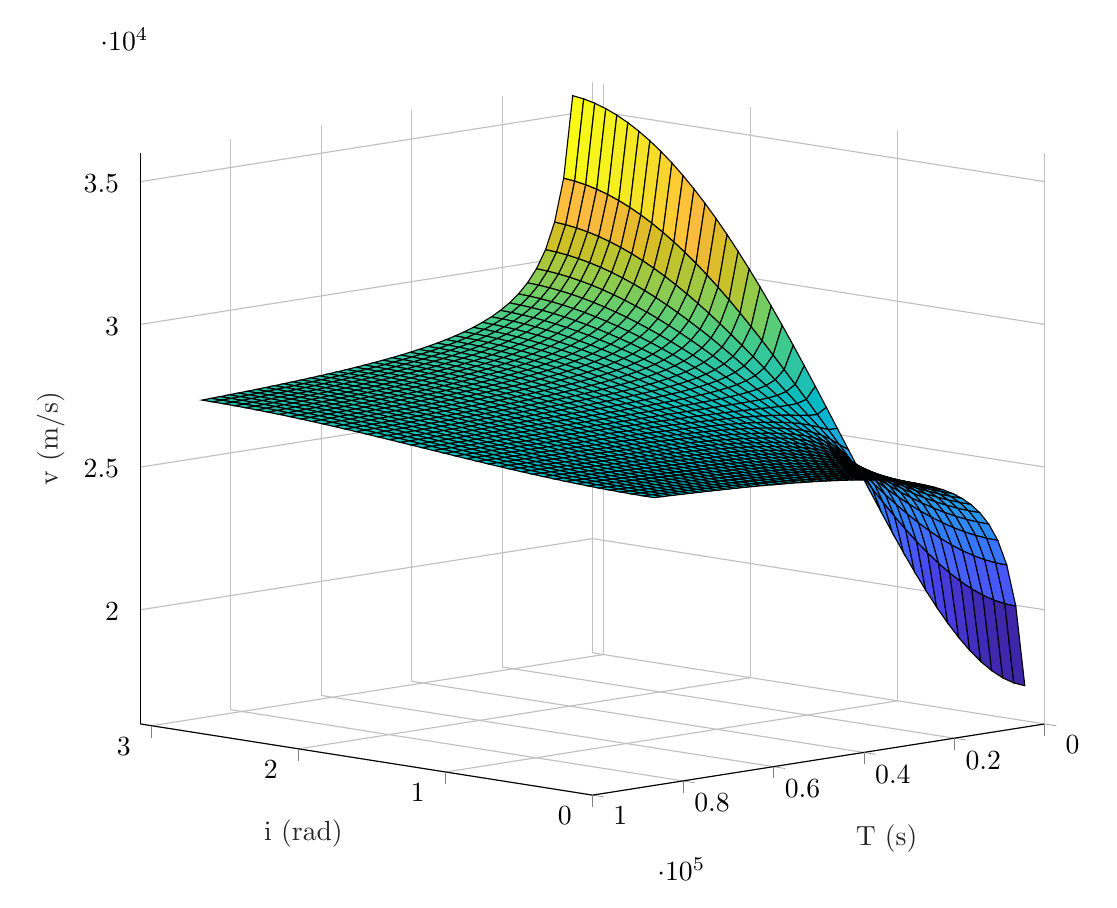
\begin{tikzpicture}

\begin{axis}[%
width=4.521in,
height=3.566in,
at={(0.758in,0.481in)},
scale only axis,
xmin=0,
xmax=3.075,
tick align=outside,
xlabel style={font=\color{white!15!black}},
xlabel={i (rad)},
ymin=0,
ymax=100000,
ylabel style={font=\color{white!15!black}},
ylabel={T (s)},
zmin=16000,
zmax=36000,
zlabel style={font=\color{white!15!black}},
zlabel={v (m/s)},
view={-135}{10},
axis background/.style={fill=white},
axis x line*=bottom,
axis y line*=left,
axis z line*=left,
xmajorgrids,
ymajorgrids,
zmajorgrids
]

\addplot3[%
surf,
shader=flat corner, draw=black, z buffer=sort, colormap={mymap}{[1pt] rgb(0pt)=(0.2422,0.1504,0.6603); rgb(1pt)=(0.2444,0.1534,0.6728); rgb(2pt)=(0.2464,0.1569,0.6847); rgb(3pt)=(0.2484,0.1607,0.6961); rgb(4pt)=(0.2503,0.1648,0.7071); rgb(5pt)=(0.2522,0.1689,0.7179); rgb(6pt)=(0.254,0.1732,0.7286); rgb(7pt)=(0.2558,0.1773,0.7393); rgb(8pt)=(0.2576,0.1814,0.7501); rgb(9pt)=(0.2594,0.1854,0.761); rgb(11pt)=(0.2628,0.1932,0.7828); rgb(12pt)=(0.2645,0.1972,0.7937); rgb(13pt)=(0.2661,0.2011,0.8043); rgb(14pt)=(0.2676,0.2052,0.8148); rgb(15pt)=(0.2691,0.2094,0.8249); rgb(16pt)=(0.2704,0.2138,0.8346); rgb(17pt)=(0.2717,0.2184,0.8439); rgb(18pt)=(0.2729,0.2231,0.8528); rgb(19pt)=(0.274,0.228,0.8612); rgb(20pt)=(0.2749,0.233,0.8692); rgb(21pt)=(0.2758,0.2382,0.8767); rgb(22pt)=(0.2766,0.2435,0.884); rgb(23pt)=(0.2774,0.2489,0.8908); rgb(24pt)=(0.2781,0.2543,0.8973); rgb(25pt)=(0.2788,0.2598,0.9035); rgb(26pt)=(0.2794,0.2653,0.9094); rgb(27pt)=(0.2798,0.2708,0.915); rgb(28pt)=(0.2802,0.2764,0.9204); rgb(29pt)=(0.2806,0.2819,0.9255); rgb(30pt)=(0.2809,0.2875,0.9305); rgb(31pt)=(0.2811,0.293,0.9352); rgb(32pt)=(0.2813,0.2985,0.9397); rgb(33pt)=(0.2814,0.304,0.9441); rgb(34pt)=(0.2814,0.3095,0.9483); rgb(35pt)=(0.2813,0.315,0.9524); rgb(36pt)=(0.2811,0.3204,0.9563); rgb(37pt)=(0.2809,0.3259,0.96); rgb(38pt)=(0.2807,0.3313,0.9636); rgb(39pt)=(0.2803,0.3367,0.967); rgb(40pt)=(0.2798,0.3421,0.9702); rgb(41pt)=(0.2791,0.3475,0.9733); rgb(42pt)=(0.2784,0.3529,0.9763); rgb(43pt)=(0.2776,0.3583,0.9791); rgb(44pt)=(0.2766,0.3638,0.9817); rgb(45pt)=(0.2754,0.3693,0.984); rgb(46pt)=(0.2741,0.3748,0.9862); rgb(47pt)=(0.2726,0.3804,0.9881); rgb(48pt)=(0.271,0.386,0.9898); rgb(49pt)=(0.2691,0.3916,0.9912); rgb(50pt)=(0.267,0.3973,0.9924); rgb(51pt)=(0.2647,0.403,0.9935); rgb(52pt)=(0.2621,0.4088,0.9946); rgb(53pt)=(0.2591,0.4145,0.9955); rgb(54pt)=(0.2556,0.4203,0.9965); rgb(55pt)=(0.2517,0.4261,0.9974); rgb(56pt)=(0.2473,0.4319,0.9983); rgb(57pt)=(0.2424,0.4378,0.9991); rgb(58pt)=(0.2369,0.4437,0.9996); rgb(59pt)=(0.2311,0.4497,0.9995); rgb(60pt)=(0.225,0.4559,0.9985); rgb(61pt)=(0.2189,0.462,0.9968); rgb(62pt)=(0.2128,0.4682,0.9948); rgb(63pt)=(0.2066,0.4743,0.9926); rgb(64pt)=(0.2006,0.4803,0.9906); rgb(65pt)=(0.195,0.4861,0.9887); rgb(66pt)=(0.1903,0.4919,0.9867); rgb(67pt)=(0.1869,0.4975,0.9844); rgb(68pt)=(0.1847,0.503,0.9819); rgb(69pt)=(0.1831,0.5084,0.9793); rgb(70pt)=(0.1818,0.5138,0.9766); rgb(71pt)=(0.1806,0.5191,0.9738); rgb(72pt)=(0.1795,0.5244,0.9709); rgb(73pt)=(0.1785,0.5296,0.9677); rgb(74pt)=(0.1778,0.5349,0.9641); rgb(75pt)=(0.1773,0.5401,0.9602); rgb(76pt)=(0.1768,0.5452,0.956); rgb(77pt)=(0.1764,0.5504,0.9516); rgb(78pt)=(0.1755,0.5554,0.9473); rgb(79pt)=(0.174,0.5605,0.9432); rgb(80pt)=(0.1716,0.5655,0.9393); rgb(81pt)=(0.1686,0.5705,0.9357); rgb(82pt)=(0.1649,0.5755,0.9323); rgb(83pt)=(0.161,0.5805,0.9289); rgb(84pt)=(0.1573,0.5854,0.9254); rgb(85pt)=(0.154,0.5902,0.9218); rgb(86pt)=(0.1513,0.595,0.9182); rgb(87pt)=(0.1492,0.5997,0.9147); rgb(88pt)=(0.1475,0.6043,0.9113); rgb(89pt)=(0.1461,0.6089,0.908); rgb(90pt)=(0.1446,0.6135,0.905); rgb(91pt)=(0.1429,0.618,0.9022); rgb(92pt)=(0.1408,0.6226,0.8998); rgb(93pt)=(0.1383,0.6272,0.8975); rgb(94pt)=(0.1354,0.6317,0.8953); rgb(95pt)=(0.1321,0.6363,0.8932); rgb(96pt)=(0.1288,0.6408,0.891); rgb(97pt)=(0.1253,0.6453,0.8887); rgb(98pt)=(0.1219,0.6497,0.8862); rgb(99pt)=(0.1185,0.6541,0.8834); rgb(100pt)=(0.1152,0.6584,0.8804); rgb(101pt)=(0.1119,0.6627,0.877); rgb(102pt)=(0.1085,0.6669,0.8734); rgb(103pt)=(0.1048,0.671,0.8695); rgb(104pt)=(0.1009,0.675,0.8653); rgb(105pt)=(0.0964,0.6789,0.8609); rgb(106pt)=(0.0914,0.6828,0.8562); rgb(107pt)=(0.0855,0.6865,0.8513); rgb(108pt)=(0.0789,0.6902,0.8462); rgb(109pt)=(0.0713,0.6938,0.8409); rgb(110pt)=(0.0628,0.6972,0.8355); rgb(111pt)=(0.0535,0.7006,0.8299); rgb(112pt)=(0.0433,0.7039,0.8242); rgb(113pt)=(0.0328,0.7071,0.8183); rgb(114pt)=(0.0234,0.7103,0.8124); rgb(115pt)=(0.0155,0.7133,0.8064); rgb(116pt)=(0.0091,0.7163,0.8003); rgb(117pt)=(0.0046,0.7192,0.7941); rgb(118pt)=(0.0019,0.722,0.7878); rgb(119pt)=(0.0009,0.7248,0.7815); rgb(120pt)=(0.0018,0.7275,0.7752); rgb(121pt)=(0.0046,0.7301,0.7688); rgb(122pt)=(0.0094,0.7327,0.7623); rgb(123pt)=(0.0162,0.7352,0.7558); rgb(124pt)=(0.0253,0.7376,0.7492); rgb(125pt)=(0.0369,0.74,0.7426); rgb(126pt)=(0.0504,0.7423,0.7359); rgb(127pt)=(0.0638,0.7446,0.7292); rgb(128pt)=(0.077,0.7468,0.7224); rgb(129pt)=(0.0899,0.7489,0.7156); rgb(130pt)=(0.1023,0.751,0.7088); rgb(131pt)=(0.1141,0.7531,0.7019); rgb(132pt)=(0.1252,0.7552,0.695); rgb(133pt)=(0.1354,0.7572,0.6881); rgb(134pt)=(0.1448,0.7593,0.6812); rgb(135pt)=(0.1532,0.7614,0.6741); rgb(136pt)=(0.1609,0.7635,0.6671); rgb(137pt)=(0.1678,0.7656,0.6599); rgb(138pt)=(0.1741,0.7678,0.6527); rgb(139pt)=(0.1799,0.7699,0.6454); rgb(140pt)=(0.1853,0.7721,0.6379); rgb(141pt)=(0.1905,0.7743,0.6303); rgb(142pt)=(0.1954,0.7765,0.6225); rgb(143pt)=(0.2003,0.7787,0.6146); rgb(144pt)=(0.2061,0.7808,0.6065); rgb(145pt)=(0.2118,0.7828,0.5983); rgb(146pt)=(0.2178,0.7849,0.5899); rgb(147pt)=(0.2244,0.7869,0.5813); rgb(148pt)=(0.2318,0.7887,0.5725); rgb(149pt)=(0.2401,0.7905,0.5636); rgb(150pt)=(0.2491,0.7922,0.5546); rgb(151pt)=(0.2589,0.7937,0.5454); rgb(152pt)=(0.2695,0.7951,0.536); rgb(153pt)=(0.2809,0.7964,0.5266); rgb(154pt)=(0.2929,0.7975,0.517); rgb(155pt)=(0.3052,0.7985,0.5074); rgb(156pt)=(0.3176,0.7994,0.4975); rgb(157pt)=(0.3301,0.8002,0.4876); rgb(158pt)=(0.3424,0.8009,0.4774); rgb(159pt)=(0.3548,0.8016,0.4669); rgb(160pt)=(0.3671,0.8021,0.4563); rgb(161pt)=(0.3795,0.8026,0.4454); rgb(162pt)=(0.3921,0.8029,0.4344); rgb(163pt)=(0.405,0.8031,0.4233); rgb(164pt)=(0.4184,0.803,0.4122); rgb(165pt)=(0.4322,0.8028,0.4013); rgb(166pt)=(0.4463,0.8024,0.3904); rgb(167pt)=(0.4608,0.8018,0.3797); rgb(168pt)=(0.4753,0.8011,0.3691); rgb(169pt)=(0.4899,0.8002,0.3586); rgb(170pt)=(0.5044,0.7993,0.348); rgb(171pt)=(0.5187,0.7982,0.3374); rgb(172pt)=(0.5329,0.797,0.3267); rgb(173pt)=(0.547,0.7957,0.3159); rgb(175pt)=(0.5748,0.7929,0.2941); rgb(176pt)=(0.5886,0.7913,0.2833); rgb(177pt)=(0.6024,0.7896,0.2726); rgb(178pt)=(0.6161,0.7878,0.2622); rgb(179pt)=(0.6297,0.7859,0.2521); rgb(180pt)=(0.6433,0.7839,0.2423); rgb(181pt)=(0.6567,0.7818,0.2329); rgb(182pt)=(0.6701,0.7796,0.2239); rgb(183pt)=(0.6833,0.7773,0.2155); rgb(184pt)=(0.6963,0.775,0.2075); rgb(185pt)=(0.7091,0.7727,0.1998); rgb(186pt)=(0.7218,0.7703,0.1924); rgb(187pt)=(0.7344,0.7679,0.1852); rgb(188pt)=(0.7468,0.7654,0.1782); rgb(189pt)=(0.759,0.7629,0.1717); rgb(190pt)=(0.771,0.7604,0.1658); rgb(191pt)=(0.7829,0.7579,0.1608); rgb(192pt)=(0.7945,0.7554,0.157); rgb(193pt)=(0.806,0.7529,0.1546); rgb(194pt)=(0.8172,0.7505,0.1535); rgb(195pt)=(0.8281,0.7481,0.1536); rgb(196pt)=(0.8389,0.7457,0.1546); rgb(197pt)=(0.8495,0.7435,0.1564); rgb(198pt)=(0.86,0.7413,0.1587); rgb(199pt)=(0.8703,0.7392,0.1615); rgb(200pt)=(0.8804,0.7372,0.165); rgb(201pt)=(0.8903,0.7353,0.1695); rgb(202pt)=(0.9,0.7336,0.1749); rgb(203pt)=(0.9093,0.7321,0.1815); rgb(204pt)=(0.9184,0.7308,0.189); rgb(205pt)=(0.9272,0.7298,0.1973); rgb(206pt)=(0.9357,0.729,0.2061); rgb(207pt)=(0.944,0.7285,0.2151); rgb(208pt)=(0.9523,0.7284,0.2237); rgb(209pt)=(0.9606,0.7285,0.2312); rgb(210pt)=(0.9689,0.7292,0.2373); rgb(211pt)=(0.977,0.7304,0.2418); rgb(212pt)=(0.9842,0.733,0.2446); rgb(213pt)=(0.99,0.7365,0.2429); rgb(214pt)=(0.9946,0.7407,0.2394); rgb(215pt)=(0.9966,0.7458,0.2351); rgb(216pt)=(0.9971,0.7513,0.2309); rgb(217pt)=(0.9972,0.7569,0.2267); rgb(218pt)=(0.9971,0.7626,0.2224); rgb(219pt)=(0.9969,0.7683,0.2181); rgb(220pt)=(0.9966,0.774,0.2138); rgb(221pt)=(0.9962,0.7798,0.2095); rgb(222pt)=(0.9957,0.7856,0.2053); rgb(223pt)=(0.9949,0.7915,0.2012); rgb(224pt)=(0.9938,0.7974,0.1974); rgb(225pt)=(0.9923,0.8034,0.1939); rgb(226pt)=(0.9906,0.8095,0.1906); rgb(227pt)=(0.9885,0.8156,0.1875); rgb(228pt)=(0.9861,0.8218,0.1846); rgb(229pt)=(0.9835,0.828,0.1817); rgb(230pt)=(0.9807,0.8342,0.1787); rgb(231pt)=(0.9778,0.8404,0.1757); rgb(232pt)=(0.9748,0.8467,0.1726); rgb(233pt)=(0.972,0.8529,0.1695); rgb(234pt)=(0.9694,0.8591,0.1665); rgb(235pt)=(0.9671,0.8654,0.1636); rgb(236pt)=(0.9651,0.8716,0.1608); rgb(237pt)=(0.9634,0.8778,0.1582); rgb(238pt)=(0.9619,0.884,0.1557); rgb(239pt)=(0.9608,0.8902,0.1532); rgb(240pt)=(0.9601,0.8963,0.1507); rgb(241pt)=(0.9596,0.9023,0.148); rgb(242pt)=(0.9595,0.9084,0.145); rgb(243pt)=(0.9597,0.9143,0.1418); rgb(244pt)=(0.9601,0.9203,0.1382); rgb(245pt)=(0.9608,0.9262,0.1344); rgb(246pt)=(0.9618,0.932,0.1304); rgb(247pt)=(0.9629,0.9379,0.1261); rgb(248pt)=(0.9642,0.9437,0.1216); rgb(249pt)=(0.9657,0.9494,0.1168); rgb(250pt)=(0.9674,0.9552,0.1116); rgb(251pt)=(0.9692,0.9609,0.1061); rgb(252pt)=(0.9711,0.9667,0.1001); rgb(253pt)=(0.973,0.9724,0.0938); rgb(254pt)=(0.9749,0.9782,0.0872); rgb(255pt)=(0.9769,0.9839,0.0805)}, mesh/rows=42]
table[row sep=crcr, point meta=\thisrow{c}] {%
%
x	y	z	c\\
0	4400	17448.0907081655	17448.0907081655\\
0	6400	20291.1467368638	20291.1467368638\\
0	8400	21780.36656142	21780.36656142\\
0	10400	22696.8095303777	22696.8095303777\\
0	12400	23317.6257351555	23317.6257351555\\
0	14400	23765.9929941617	23765.9929941617\\
0	16400	24105.0023851176	24105.0023851176\\
0	18400	24370.3140823874	24370.3140823874\\
0	20400	24583.6038782318	24583.6038782318\\
0	22400	24758.8062105325	24758.8062105325\\
0	24400	24905.2868490134	24905.2868490134\\
0	26400	25029.5734513609	25029.5734513609\\
0	28400	25136.3548984482	25136.3548984482\\
0	30400	25229.0861551292	25229.0861551292\\
0	32400	25310.3691085163	25310.3691085163\\
0	34400	25382.2005556956	25382.2005556956\\
0	36400	25446.1384372508	25446.1384372508\\
0	38400	25503.4161228106	25503.4161228106\\
0	40400	25555.0227503943	25555.0227503943\\
0	42400	25601.7608282058	25601.7608282058\\
0	44400	25644.2882683768	25644.2882683768\\
0	46400	25683.1495499122	25683.1495499122\\
0	48400	25718.7991552878	25718.7991552878\\
0	50400	25751.6194269033	25751.6194269033\\
0	52400	25781.9343342734	25781.9343342734\\
0	54400	25810.0202043369	25810.0202043369\\
0	56400	25836.1141687221	25836.1141687221\\
0	58400	25860.4208752727	25860.4208752727\\
0	60400	25883.1178661578	25883.1178661578\\
0	62400	25904.3599217296	25904.3599217296\\
0	64400	25924.2825949678	25924.2825949678\\
0	66400	25943.0051071676	25943.0051071676\\
0	68400	25960.632735613	25960.632735613\\
0	70400	25977.2587942603	25977.2587942603\\
0	72400	25992.9662861316	25992.9662861316\\
0	74400	26007.8292891926	26007.8292891926\\
0	76400	26021.914124554	26021.914124554\\
0	78400	26035.2803458664	26035.2803458664\\
0	80400	26047.9815810439	26047.9815810439\\
0	82400	26060.0662514069	26060.0662514069\\
0	84400	26071.5781885774	26071.5781885774\\
0	86400	26082.5571656936	26082.5571656936\\
0.075	4400	17486.9585066467	17486.9585066467\\
0.075	6400	20314.1368684039	20314.1368684039\\
0.075	8400	21796.6883150009	21796.6883150009\\
0.075	10400	22709.4614027648	22709.4614027648\\
0.075	12400	23327.9550564922	23327.9550564922\\
0.075	14400	23774.7202115378	23774.7202115378\\
0.075	16400	24112.5577405413	24112.5577405413\\
0.075	18400	24376.9750249103	24376.9750249103\\
0.075	20400	24589.5597544151	24589.5597544151\\
0.075	22400	24764.1919957528	24764.1919957528\\
0.075	24400	24910.2021458952	24910.2021458952\\
0.075	26400	25034.0938568293	25034.0938568293\\
0.075	28400	25140.5391443341	25140.5391443341\\
0.075	30400	25232.9807775469	25232.9807775469\\
0.075	32400	25314.0116058664	25314.0116058664\\
0.075	34400	25385.621586639	25385.621586639\\
0.075	36400	25449.3633887961	25449.3633887961\\
0.075	38400	25506.4662533861	25506.4662533861\\
0.075	40400	25557.9160390304	25557.9160390304\\
0.075	42400	25604.5126160676	25604.5126160676\\
0.075	44400	25646.9117507351	25646.9117507351\\
0.075	46400	25685.6561585328	25685.6561585328\\
0.075	48400	25721.1988592769	25721.1988592769\\
0.075	50400	25753.920972025	25753.920972025\\
0.075	52400	25784.1454352438	25784.1454352438\\
0.075	54400	25812.1477007645	25812.1477007645\\
0.075	56400	25838.1641526411	25838.1641526411\\
0.075	58400	25862.3987962601	25862.3987962601\\
0.075	60400	25885.0286186025	25885.0286186025\\
0.075	62400	25906.2079177704	25906.2079177704\\
0.075	64400	25926.0718258338	25926.0718258338\\
0.075	66400	25944.739195067	25944.739195067\\
0.075	68400	25962.3149778651	25962.3149778651\\
0.075	70400	25978.8922010211	25978.8922010211\\
0.075	72400	25994.5536127987	25994.5536127987\\
0.075	74400	26009.3730643642	26009.3730643642\\
0.075	76400	26023.4166742551	26023.4166742551\\
0.075	78400	26036.7438146242	26036.7438146242\\
0.075	80400	26049.407950292	26049.407950292\\
0.075	82400	26061.4573556142	26061.4573556142\\
0.075	84400	26072.9357294316	26072.9357294316\\
0.075	86400	26083.8827246137	26083.8827246137\\
0.15	4400	17602.8301376135	17602.8301376135\\
0.15	6400	20382.8229288434	20382.8229288434\\
0.15	8400	21845.4888804821	21845.4888804821\\
0.15	10400	22747.3038036639	22747.3038036639\\
0.15	12400	23358.8576292804	23358.8576292804\\
0.15	14400	23800.8336585868	23800.8336585868\\
0.15	16400	24135.1671834386	24135.1671834386\\
0.15	18400	24396.9095264134	24396.9095264134\\
0.15	20400	24607.3852759849	24607.3852759849\\
0.15	22400	24780.3120702655	24780.3120702655\\
0.15	24400	24924.9146041112	24924.9146041112\\
0.15	26400	25047.6247790608	25047.6247790608\\
0.15	28400	25153.0641939965	25153.0641939965\\
0.15	30400	25244.6391545677	25244.6391545677\\
0.15	32400	25324.915485358	25324.915485358\\
0.15	34400	25395.8626892045	25395.8626892045\\
0.15	36400	25459.0176685422	25459.0176685422\\
0.15	38400	25515.5973156651	25515.5973156651\\
0.15	40400	25566.5776797098	25566.5776797098\\
0.15	42400	25612.7507400307	25612.7507400307\\
0.15	44400	25654.7658432332	25654.7658432332\\
0.15	46400	25693.1604288782	25693.1604288782\\
0.15	48400	25728.3831407043	25728.3831407043\\
0.15	50400	25760.8114375493	25760.8114375493\\
0.15	52400	25790.7651728918	25790.7651728918\\
0.15	54400	25818.5171800761	25818.5171800761\\
0.15	56400	25844.3016062048	25844.3016062048\\
0.15	58400	25868.3205342002	25868.3205342002\\
0.15	60400	25890.7492896763	25890.7492896763\\
0.15	62400	25911.7407275962	25911.7407275962\\
0.15	64400	25931.4287204263	25931.4287204263\\
0.15	66400	25949.9310160948	25949.9310160948\\
0.15	68400	25967.3515947024	25967.3515947024\\
0.15	70400	25983.7826236348	25983.7826236348\\
0.15	72400	25999.3060887144	25999.3060887144\\
0.15	74400	26013.9951623317	26013.9951623317\\
0.15	76400	26027.9153567443	26027.9153567443\\
0.15	78400	26041.1255008938	26041.1255008938\\
0.15	80400	26053.6785714655	26053.6785714655\\
0.15	82400	26065.6224029484	26065.6224029484\\
0.15	84400	26077.0002967625	26077.0002967625\\
0.15	86400	26087.8515458033	26087.8515458033\\
0.225	4400	17793.5590158599	17793.5590158599\\
0.225	6400	20496.3621442116	20496.3621442116\\
0.225	8400	21926.2783441652	21926.2783441652\\
0.225	10400	22809.9993578306	22809.9993578306\\
0.225	12400	23410.0787308098	23410.0787308098\\
0.225	14400	23844.1297410816	23844.1297410816\\
0.225	16400	24172.661610842	24172.661610842\\
0.225	18400	24429.973212629	24429.973212629\\
0.225	20400	24636.9546141835	24636.9546141835\\
0.225	22400	24807.0550025431	24807.0550025431\\
0.225	24400	24949.3242784169	24949.3242784169\\
0.225	26400	25070.0756415324	25070.0756415324\\
0.225	28400	25173.8472531383	25173.8472531383\\
0.225	30400	25263.9850559465	25263.9850559465\\
0.225	32400	25343.0101258008	25343.0101258008\\
0.225	34400	25412.8580891407	25412.8580891407\\
0.225	36400	25475.0397315437	25475.0397315437\\
0.225	38400	25530.7514866848	25530.7514866848\\
0.225	40400	25580.9531497627	25580.9531497627\\
0.225	42400	25626.4236234991	25626.4236234991\\
0.225	44400	25667.8016149908	25667.8016149908\\
0.225	46400	25705.6158189355	25705.6158189355\\
0.225	48400	25740.3076250969	25740.3076250969\\
0.225	50400	25772.2484244984	25772.2484244984\\
0.225	52400	25801.7529560404	25801.7529560404\\
0.225	54400	25829.0897116139	25829.0897116139\\
0.225	56400	25854.4891292313	25854.4891292313\\
0.225	58400	25878.1501039993	25878.1501039993\\
0.225	60400	25900.2452065256	25900.2452065256\\
0.225	62400	25920.9248985353	25920.9248985353\\
0.225	64400	25940.3209635319	25940.3209635319\\
0.225	66400	25958.5493178893	25958.5493178893\\
0.225	68400	25975.7123290992	25975.7123290992\\
0.225	70400	25991.9007391174	25991.9007391174\\
0.225	72400	26007.1952691234	26007.1952691234\\
0.225	74400	26021.6679656033	26021.6679656033\\
0.225	76400	26035.3833351309	26035.3833351309\\
0.225	78400	26048.3993055565	26048.3993055565\\
0.225	80400	26060.7680438134	26060.7680438134\\
0.225	82400	26072.5366546913	26072.5366546913\\
0.225	84400	26083.7477803091	26083.7477803091\\
0.225	86400	26094.4401163704	26094.4401163704\\
0.3	4400	18055.7221231469	18055.7221231469\\
0.3	6400	20653.3830864615	20653.3830864615\\
0.3	8400	22038.2538315857	22038.2538315857\\
0.3	10400	22896.9932411538	22896.9932411538\\
0.3	12400	23481.1986010328	23481.1986010328\\
0.3	14400	23904.2725029641	23904.2725029641\\
0.3	16400	24224.7617178518	24224.7617178518\\
0.3	18400	24475.9274559456	24475.9274559456\\
0.3	20400	24678.0596823788	24678.0596823788\\
0.3	22400	24844.2364366274	24844.2364366274\\
0.3	24400	24983.2657590535	24983.2657590535\\
0.3	26400	25101.2964969619	25101.2964969619\\
0.3	28400	25202.7512248837	25202.7512248837\\
0.3	30400	25290.8922282441	25290.8922282441\\
0.3	32400	25368.1785429299	25368.1785429299\\
0.3	34400	25436.4988144368	25436.4988144368\\
0.3	36400	25497.3275989816	25497.3275989816\\
0.3	38400	25551.832943446	25551.832943446\\
0.3	40400	25600.9520857526	25600.9520857526\\
0.3	42400	25645.4457775683	25645.4457775683\\
0.3	44400	25685.9379554306	25685.9379554306\\
0.3	46400	25722.9451720258	25722.9451720258\\
0.3	48400	25756.898743864	25756.898743864\\
0.3	50400	25788.1616348923	25788.1616348923\\
0.3	52400	25817.0414800475	25817.0414800475\\
0.3	54400	25843.8007405111	25843.8007405111\\
0.3	56400	25868.6647015402	25868.6647015402\\
0.3	58400	25891.8278292881	25891.8278292881\\
0.3	60400	25913.458866436	25913.458866436\\
0.3	62400	25933.7049492042	25933.7049492042\\
0.3	64400	25952.6949582044	25952.6949582044\\
0.3	66400	25970.5422644666	25970.5422644666\\
0.3	68400	25987.3469942828	25987.3469942828\\
0.3	70400	26003.1979084443	26003.1979084443\\
0.3	72400	26018.1739703512	26018.1739703512\\
0.3	74400	26032.3456614749	26032.3456614749\\
0.3	76400	26045.7760904201	26045.7760904201\\
0.3	78400	26058.5219324057	26058.5219324057\\
0.3	80400	26070.6342286632	26070.6342286632\\
0.3	82400	26082.1590695294	26082.1590695294\\
0.3	84400	26093.1381805086	26093.1381805086\\
0.3	86400	26103.6094270105	26103.6094270105\\
0.375	4400	18384.8270232019	18384.8270232019\\
0.375	6400	20852.0324590772	20852.0324590772\\
0.375	8400	22180.3191043491	22180.3191043491\\
0.375	10400	23007.5240057497	23007.5240057497\\
0.375	12400	23571.6394082078	23571.6394082078\\
0.375	14400	23980.7985551792	23980.7985551792\\
0.375	16400	24291.0817158082	24291.0817158082\\
0.375	18400	24534.442311315	24534.442311315\\
0.375	20400	24730.4125343881	24730.4125343881\\
0.375	22400	24891.6011031543	24891.6011031543\\
0.375	24400	25026.5098931571	25026.5098931571\\
0.375	26400	25141.0795255332	25141.0795255332\\
0.375	28400	25239.5860317026	25239.5860317026\\
0.375	30400	25325.185574574	25325.185574574\\
0.375	32400	25400.2584524607	25400.2584524607\\
0.375	34400	25466.6336611537	25466.6336611537\\
0.375	36400	25525.7397419264	25525.7397419264\\
0.375	38400	25578.7086766087	25578.7086766087\\
0.375	40400	25626.4490367465	25626.4490367465\\
0.375	42400	25669.6985017195	25669.6985017195\\
0.375	44400	25709.0622288612	25709.0622288612\\
0.375	46400	25745.0413306581	25745.0413306581\\
0.375	48400	25778.0543119407	25778.0543119407\\
0.375	50400	25808.4534170147	25808.4534170147\\
0.375	52400	25836.5372429659	25836.5372429659\\
0.375	54400	25862.5605775604	25862.5605775604\\
0.375	56400	25886.7421489658	25886.7421489658\\
0.375	58400	25909.2707867004	25909.2707867004\\
0.375	60400	25930.3103612349	25930.3103612349\\
0.375	62400	25950.0037756708	25950.0037756708\\
0.375	64400	25968.4762151353	25968.4762151353\\
0.375	66400	25985.8378100835	25985.8378100835\\
0.375	68400	26002.1858332358	26002.1858332358\\
0.375	70400	26017.6065227188	26017.6065227188\\
0.375	72400	26032.176603562	26032.176603562\\
0.375	74400	26045.96456421	26045.96456421\\
0.375	76400	26059.0317328669	26059.0317328669\\
0.375	78400	26071.4331893597	26071.4331893597\\
0.375	80400	26083.218541114	26083.218541114\\
0.375	82400	26094.4325862956	26094.4325862956\\
0.375	84400	26105.1158828047	26105.1158828047\\
0.375	86400	26115.3052383578	26115.3052383578\\
0.45	4400	18775.5587034662	18775.5587034662\\
0.45	6400	21090.0350614444	21090.0350614444\\
0.45	8400	22351.110344724	22351.110344724\\
0.45	10400	23140.6380158126	23140.6380158126\\
0.45	12400	23680.6746141404	23680.6746141404\\
0.45	14400	24073.1237389818	24073.1237389818\\
0.45	16400	24371.1343788466	24371.1343788466\\
0.45	18400	24605.1005130122	24605.1005130122\\
0.45	20400	24793.6486370724	24793.6486370724\\
0.45	22400	24948.8255686571	24948.8255686571\\
0.45	24400	25078.7661417888	25078.7661417888\\
0.45	26400	25189.1610890126	25189.1610890126\\
0.45	28400	25284.1104298278	25284.1104298278\\
0.45	30400	25366.6427754202	25366.6427754202\\
0.45	32400	25439.0437318071	25439.0437318071\\
0.45	34400	25503.0705224306	25503.0705224306\\
0.45	36400	25560.0962982072	25560.0962982072\\
0.45	38400	25611.2096115335	25611.2096115335\\
0.45	40400	25657.2845026469	25657.2845026469\\
0.45	42400	25699.0308501338	25699.0308501338\\
0.45	44400	25737.0311775868	25737.0311775868\\
0.45	46400	25771.7679837745	25771.7679837745\\
0.45	48400	25803.6443253437	25803.6443253437\\
0.45	50400	25832.9995185118	25832.9995185118\\
0.45	52400	25860.1212586578	25860.1212586578\\
0.45	54400	25885.255076193	25885.255076193\\
0.45	56400	25908.6117875357	25908.6117875357\\
0.45	58400	25930.3734201577	25930.3734201577\\
0.45	60400	25950.6979642284	25950.6979642284\\
0.45	62400	25969.7232132847	25969.7232132847\\
0.45	64400	25987.5698913613	25987.5698913613\\
0.45	66400	26004.3442165865	26004.3442165865\\
0.45	68400	26020.1400162596	26020.1400162596\\
0.45	70400	26035.0404823607	26035.0404823607\\
0.45	72400	26049.1196368396	26049.1196368396\\
0.45	74400	26062.4435611562	26062.4435611562\\
0.45	76400	26075.0714331639	26075.0714331639\\
0.45	78400	26087.0564056588	26087.0564056588\\
0.45	80400	26098.4463540998	26098.4463540998\\
0.45	82400	26109.2845156778	26109.2845156778\\
0.45	84400	26119.6100377173	26119.6100377173\\
0.45	86400	26129.4584500707	26129.4584500707\\
0.525	4400	19222.0364683636	19222.0364683636\\
0.525	6400	21364.7623981771	21364.7623981771\\
0.525	8400	22549.0266936865	22549.0266936865\\
0.525	10400	23295.2068503805	23295.2068503805\\
0.525	12400	23807.4403865996	23807.4403865996\\
0.525	14400	24180.5513049948	24180.5513049948\\
0.525	16400	24464.3372709535	24464.3372709535\\
0.525	18400	24687.4024258949	24687.4024258949\\
0.525	20400	24867.3309370892	24867.3309370892\\
0.525	22400	25015.5216605958	25015.5216605958\\
0.525	24400	25139.6855223325	25139.6855223325\\
0.525	26400	25245.2242994365	25245.2242994365\\
0.525	28400	25336.0342815342	25336.0342815342\\
0.525	30400	25414.9963210391	25414.9963210391\\
0.525	32400	25484.286255006	25484.286255006\\
0.525	34400	25545.5780584337	25545.5780584337\\
0.525	36400	25600.1806027716	25600.1806027716\\
0.525	38400	25649.1320192096	25649.1320192096\\
0.525	40400	25693.266241926	25693.266241926\\
0.525	42400	25733.2608494817	25733.2608494817\\
0.525	44400	25769.6720606874	25769.6720606874\\
0.525	46400	25802.9607356411	25802.9607356411\\
0.525	48400	25833.5119678456	25833.5119678456\\
0.525	50400	25861.650037366	25861.650037366\\
0.525	52400	25887.6499576399	25887.6499576399\\
0.525	54400	25911.7464879949	25911.7464879949\\
0.525	56400	25934.1412378174	25934.1412378174\\
0.525	58400	25955.008317673	25955.008317673\\
0.525	60400	25974.4988726428	25974.4988726428\\
0.525	62400	25992.74474756	25992.74474756\\
0.525	64400	26009.8614720703	26009.8614720703\\
0.525	66400	26025.9507083465	26025.9507083465\\
0.525	68400	26041.1022710092	26041.1022710092\\
0.525	70400	26055.3958040057	26055.3958040057\\
0.525	72400	26068.9021805406	26068.9021805406\\
0.525	74400	26081.6846779862	26081.6846779862\\
0.525	76400	26093.7999688678	26093.7999688678\\
0.525	78400	26105.2989606573	26105.2989606573\\
0.525	80400	26116.2275106186	26116.2275106186\\
0.525	82400	26126.6270368667	26126.6270368667\\
0.525	84400	26136.5350428047	26136.5350428047\\
0.525	86400	26145.9855689326	26145.9855689326\\
0.6	4400	19718.0558094738	19718.0558094738\\
0.6	6400	21673.3052759432	21673.3052759432\\
0.6	8400	22772.2639666923	22772.2639666923\\
0.6	10400	23469.9469414619	23469.9469414619\\
0.6	12400	23950.9486502572	23950.9486502572\\
0.6	14400	24302.2813509259	24302.2813509259\\
0.6	16400	24570.0199779762	24570.0199779762\\
0.6	18400	24780.7718239672	24780.7718239672\\
0.6	20400	24950.9546254282	24950.9546254282\\
0.6	22400	25091.2404925063	25091.2404925063\\
0.6	24400	25208.8640752814	25208.8640752814\\
0.6	26400	25308.9020520698	25308.9020520698\\
0.6	28400	25395.0212430076	25395.0212430076\\
0.6	30400	25469.9359193549	25469.9359193549\\
0.6	32400	25535.6980696264	25535.6980696264\\
0.6	34400	25593.887679928	25593.887679928\\
0.6	36400	25645.7410073923	25645.7410073923\\
0.6	38400	25692.2391955454	25692.2391955454\\
0.6	40400	25734.1708294261	25734.1708294261\\
0.6	42400	25772.1769507003	25772.1769507003\\
0.6	44400	25806.7840125587	25806.7840125587\\
0.6	46400	25838.4283818266	25838.4283818266\\
0.6	48400	25867.4748133908	25867.4748133908\\
0.6	50400	25894.230558393	25894.230558393\\
0.6	52400	25918.9562642079	25918.9562642079\\
0.6	54400	25941.8744861019	25941.8744861019\\
0.6	56400	25963.176399481	25963.176399481\\
0.6	58400	25983.0271413554	25983.0271413554\\
0.6	60400	26001.5700968207	26001.5700968207\\
0.6	62400	26018.9303658697	26018.9303658697\\
0.6	64400	26035.2175877239	26035.2175877239\\
0.6	66400	26050.5282574174	26050.5282574174\\
0.6	68400	26064.9476380165	26064.9476380165\\
0.6	70400	26078.5513484846	26078.5513484846\\
0.6	72400	26091.4066896088	26091.4066896088\\
0.6	74400	26103.5737570458	26103.5737570458\\
0.6	76400	26115.1063803191	26115.1063803191\\
0.6	78400	26126.0529187115	26126.0529187115\\
0.6	80400	26136.4569388628	26136.4569388628\\
0.6	82400	26146.3577940912	26146.3577940912\\
0.6	84400	26155.79112167	26155.79112167\\
0.6	86400	26164.7892713059	26164.7892713059\\
0.675	4400	20257.2980724346	20257.2980724346\\
0.675	6400	22012.5461222359	22012.5461222359\\
0.675	8400	23018.8499699623	23018.8499699623\\
0.675	10400	23663.4406826717	23663.4406826717\\
0.675	12400	24110.1013376433	24110.1013376433\\
0.675	14400	24437.4212372323	24437.4212372323\\
0.675	16400	24687.432150513	24687.432150513\\
0.675	18400	24884.5623543033	24884.5623543033\\
0.675	20400	25043.9524913812	25043.9524913812\\
0.675	22400	25175.4770037607	25175.4770037607\\
0.675	24400	25285.846786106	25285.846786106\\
0.675	26400	25379.7804652231	25379.7804652231\\
0.675	28400	25460.6918193789	25460.6918193789\\
0.675	30400	25531.1112378833	25531.1112378833\\
0.675	32400	25592.9538796946	25592.9538796946\\
0.675	34400	25647.6958139195	25647.6958139195\\
0.675	36400	25696.4929617761	25696.4929617761\\
0.675	38400	25740.2633840644	25740.2633840644\\
0.675	40400	25779.7454417676	25779.7454417676\\
0.675	42400	25815.5396944158	25815.5396944158\\
0.675	44400	25848.1396026756	25848.1396026756\\
0.675	46400	25877.95437529	25877.95437529\\
0.675	48400	25905.3262086205	25905.3262086205\\
0.675	50400	25930.5434608115	25930.5434608115\\
0.675	52400	25953.8508364285	25953.8508364285\\
0.675	54400	25975.4573439826	25975.4573439826\\
0.675	56400	25995.5425744055	25995.5425744055\\
0.675	58400	26014.261699672	26014.261699672\\
0.675	60400	26031.7494858843	26031.7494858843\\
0.675	62400	26048.1235402576	26048.1235402576\\
0.675	64400	26063.4869573406	26063.4869573406\\
0.675	66400	26077.9304902497	26077.9304902497\\
0.675	68400	26091.5343434809	26091.5343434809\\
0.675	70400	26104.3696620637	26104.3696620637\\
0.675	72400	26116.4997754053	26116.4997754053\\
0.675	74400	26127.9812417051	26127.9812417051\\
0.675	76400	26138.8647292669	26138.8647292669\\
0.675	78400	26149.1957636706	26149.1957636706\\
0.675	80400	26159.0153640286	26159.0153640286\\
0.675	82400	26168.3605870721	26168.3605870721\\
0.675	84400	26177.2649942746	26177.2649942746\\
0.675	86400	26185.7590544219	26185.7590544219\\
0.75	4400	20833.4992004894	20833.4992004894\\
0.75	6400	22379.2275191913	22379.2275191913\\
0.75	8400	23286.6799591188	23286.6799591188\\
0.75	10400	23874.1582611626	23874.1582611626\\
0.75	12400	24283.7053976324	24283.7053976324\\
0.75	14400	24584.9966913473	24584.9966913473\\
0.75	16400	24815.7521545254	24815.7521545254\\
0.75	18400	24998.0645360162	24998.0645360162\\
0.75	20400	25145.7007501704	25145.7007501704\\
0.75	22400	25267.6749219023	25267.6749219023\\
0.75	24400	25370.1318871553	25370.1318871553\\
0.75	26400	25457.4026644473	25457.4026644473\\
0.75	28400	25532.6267339976	25532.6267339976\\
0.75	30400	25598.1349341899	25598.1349341899\\
0.75	32400	25655.6937950409	25655.6937950409\\
0.75	34400	25706.6664165385	25706.6664165385\\
0.75	36400	25752.1213251472	25752.1213251472\\
0.75	38400	25792.9079143157	25792.9079143157\\
0.75	40400	25829.7098453957	25829.7098453957\\
0.75	42400	25863.0835673483	25863.0835673483\\
0.75	44400	25893.4865758927	25893.4865758927\\
0.75	46400	25921.2984635965	25921.2984635965\\
0.75	48400	25946.8368180134	25946.8368180134\\
0.75	50400	25970.3693806904	25970.3693806904\\
0.75	52400	25992.1234539493	25992.1234539493\\
0.75	54400	26012.2932555748	26012.2932555748\\
0.75	56400	26031.0457251977	26031.0457251977\\
0.75	58400	26048.5251496484	26048.5251496484\\
0.75	60400	26064.8568782747	26064.8568782747\\
0.75	62400	26080.1503304329	26080.1503304329\\
0.75	64400	26094.5014475998	26094.5014475998\\
0.75	66400	26107.9947061607	26107.9947061607\\
0.75	68400	26120.7047800201	26120.7047800201\\
0.75	70400	26132.6979220957	26132.6979220957\\
0.75	72400	26144.033118619	26144.033118619\\
0.75	74400	26154.7630586633	26154.7630586633\\
0.75	76400	26164.9349525028	26164.9349525028\\
0.75	78400	26174.5912256018	26174.5912256018\\
0.75	80400	26183.7701097367	26183.7701097367\\
0.75	82400	26192.5061486087	26192.5061486087\\
0.75	84400	26200.8306320372	26200.8306320372\\
0.75	86400	26208.77197023	26208.77197023\\
0.825	4400	21440.5759688309	21440.5759688309\\
0.825	6400	22770.0143939544	22770.0143939544\\
0.825	8400	23573.5509903725	23573.5509903725\\
0.825	10400	24100.4795260126	24100.4795260126\\
0.825	12400	24470.4881381711	24470.4881381711\\
0.825	14400	24743.9633163383	24743.9633163383\\
0.825	16400	24954.0961264981	24954.0961264981\\
0.825	18400	25120.5131418601	25120.5131418601\\
0.825	20400	25255.5252255724	25255.5252255724\\
0.825	22400	25367.2320524018	25367.2320524018\\
0.825	24400	25461.1754614468	25461.1754614468\\
0.825	26400	25541.2728456553	25541.2728456553\\
0.825	28400	25610.3705562161	25610.3705562161\\
0.825	30400	25670.5859267716	25670.5859267716\\
0.825	32400	25723.526305032	25723.526305032\\
0.825	34400	25770.4336960565	25770.4336960565\\
0.825	36400	25812.2828752546	25812.2828752546\\
0.825	38400	25849.8495263299	25849.8495263299\\
0.825	40400	25883.7585604444	25883.7585604444\\
0.825	42400	25914.5190253032	25914.5190253032\\
0.825	44400	25942.5497509664	25942.5497509664\\
0.825	46400	25968.1984767492	25968.1984767492\\
0.825	48400	25991.7563126975	25991.7563126975\\
0.825	50400	26013.4688107086	26013.4688107086\\
0.825	52400	26033.5445372796	26033.5445372796\\
0.825	54400	26052.1617815091	26052.1617815091\\
0.825	56400	26069.473854824	26069.473854824\\
0.825	58400	26085.6133155695	26085.6133155695\\
0.825	60400	26100.6953645093	26100.6953645093\\
0.825	62400	26114.8205949948	26114.8205949948\\
0.825	64400	26128.0772364536	26128.0772364536\\
0.825	66400	26140.5429968319	26140.5429968319\\
0.825	68400	26152.286585187	26152.286585187\\
0.825	70400	26163.3689773728	26163.3689773728\\
0.825	72400	26173.8444739975	26173.8444739975\\
0.825	74400	26183.7615893588	26183.7615893588\\
0.825	76400	26193.163802039	26193.163802039\\
0.825	78400	26202.0901916361	26202.0901916361\\
0.825	80400	26210.5759812828	26210.5759812828\\
0.825	82400	26218.6530018223	26218.6530018223\\
0.825	84400	26226.3500905271	26226.3500905271\\
0.825	86400	26233.6934348807	26233.6934348807\\
0.9	4400	22072.7130608238	22072.7130608238\\
0.9	6400	23181.5482818596	23181.5482818596\\
0.9	8400	23877.1941760157	23877.1941760157\\
0.9	10400	24340.7152981539	24340.7152981539\\
0.9	12400	24669.1125180172	24669.1125180172\\
0.9	14400	24913.2182371257	24913.2182371257\\
0.9	16400	25101.5272380589	25101.5272380589\\
0.9	18400	25251.0948137035	25251.0948137035\\
0.9	20400	25372.7077702379	25372.7077702379\\
0.9	22400	25473.5058008159	25473.5058008159\\
0.9	24400	25558.3962696571	25558.3962696571\\
0.9	26400	25630.8605508006	25630.8605508006\\
0.9	28400	25693.4355308375	25693.4355308375\\
0.9	30400	25748.0128570247	25748.0128570247\\
0.9	32400	25796.031433391	25796.031433391\\
0.9	34400	25838.6050076637	25838.6050076637\\
0.9	36400	25876.6089805037	25876.6089805037\\
0.9	38400	25910.74085023	25910.74085023\\
0.9	40400	25941.5631724108	25941.5631724108\\
0.9	42400	25969.5346572053	25969.5346572053\\
0.9	44400	25995.0330538796	25995.0330538796\\
0.9	46400	26018.3722440579	26018.3722440579\\
0.9	48400	26039.8151829697	26039.8151829697\\
0.9	50400	26059.5838186828	26059.5838186828\\
0.9	52400	26077.866781252	26077.866781252\\
0.9	54400	26094.8254052467	26094.8254052467\\
0.9	56400	26110.5984921791	26110.5984921791\\
0.9	58400	26125.3061099072	26125.3061099072\\
0.9	60400	26139.0526486928	26139.0526486928\\
0.9	62400	26151.9292981563	26151.9292981563\\
0.9	64400	26164.0160691826	26164.0160691826\\
0.9	66400	26175.3834553773	26175.3834553773\\
0.9	68400	26186.0938068509	26186.0938068509\\
0.9	70400	26196.2024727926	26196.2024727926\\
0.9	72400	26205.7587569809	26205.7587569809\\
0.9	74400	26214.8067210006	26214.8067210006\\
0.9	76400	26223.3858627463	26223.3858627463\\
0.9	78400	26231.5316922266	26231.5316922266\\
0.9	80400	26239.2762223551	26239.2762223551\\
0.9	82400	26246.6483890159	26246.6483890159\\
0.9	84400	26253.6744120131	26253.6744120131\\
0.9	86400	26260.3781063861	26260.3781063861\\
0.975	4400	22724.4170469356	22724.4170469356\\
0.975	6400	23610.4929569732	23610.4929569732\\
0.975	8400	24195.304136031	24195.304136031\\
0.975	10400	24593.1276381649	24593.1276381649\\
0.975	12400	24878.1920539422	24878.1920539422\\
0.975	14400	25091.6116440983	25091.6116440983\\
0.975	16400	25257.0649897898	25257.0649897898\\
0.975	18400	25388.9557717195	25388.9557717195\\
0.975	20400	25496.4928115352	25496.4928115352\\
0.975	22400	25585.8188353951	25585.8188353951\\
0.975	24400	25661.1807234195	25661.1807234195\\
0.975	26400	25725.6050907298	25725.6050907298\\
0.975	28400	25781.3055528373	25781.3055528373\\
0.975	30400	25829.9376930735	25829.9376930735\\
0.975	32400	25872.7640306749	25872.7640306749\\
0.975	34400	25910.7638813399	25910.7638813399\\
0.975	36400	25944.7084005081	25944.7084005081\\
0.975	38400	25975.2130096295	25975.2130096295\\
0.975	40400	26002.7747631091	26002.7747631091\\
0.975	42400	26027.7994640786	26027.7994640786\\
0.975	44400	26050.6216619737	26050.6216619737\\
0.975	46400	26071.5196178862	26071.5196178862\\
0.975	48400	26090.7266539683	26090.7266539683\\
0.975	50400	26108.4398657267	26108.4398657267\\
0.975	52400	26124.8268847895	26124.8268847895\\
0.975	54400	26140.031182381	26140.031182381\\
0.975	56400	26154.1762678508	26154.1762678508\\
0.975	58400	26167.3690416373	26167.3690416373\\
0.975	60400	26179.702494765	26179.702494765\\
0.975	62400	26191.2578986956	26191.2578986956\\
0.975	64400	26202.106594303	26202.106594303\\
0.975	66400	26212.3114630098	26212.3114630098\\
0.975	68400	26221.9281440403	26221.9281440403\\
0.975	70400	26231.0060474554	26231.0060474554\\
0.975	72400	26239.5892018377	26239.5892018377\\
0.975	74400	26247.7169672677	26247.7169672677\\
0.975	76400	26255.424637913	26255.424637913\\
0.975	78400	26262.7439536611	26262.7439536611\\
0.975	80400	26269.7035364148	26269.7035364148\\
0.975	82400	26276.3292636794	26276.3292636794\\
0.975	84400	26282.6445897066	26282.6445897066\\
0.975	86400	26288.6708225862	26288.6708225862\\
1.05	4400	23390.5442588925	23390.5442588925\\
1.05	6400	24053.5714336071	24053.5714336071\\
1.05	8400	24525.5652073908	24525.5652073908\\
1.05	10400	24855.9487070767	24855.9487070767\\
1.05	12400	25096.3050697056	25096.3050697056\\
1.05	14400	25277.9580272477	25277.9580272477\\
1.05	16400	25419.6943738621	25419.6943738621\\
1.05	18400	25533.2094896929	25533.2094896929\\
1.05	20400	25626.0939189816	25626.0939189816\\
1.05	22400	25703.4648037528	25703.4648037528\\
1.05	24400	25768.8879318711	25768.8879318711\\
1.05	26400	25824.9200525038	25824.9200525038\\
1.05	28400	25873.4402328458	25873.4402328458\\
1.05	30400	25915.8594275423	25915.8594275423\\
1.05	32400	25953.2571618864	25953.2571618864\\
1.05	34400	25986.4731447623	25986.4731447623\\
1.05	36400	26016.1701807475	26016.1701807475\\
1.05	38400	26042.8783176711	26042.8783176711\\
1.05	40400	26067.0264324672	26067.0264324672\\
1.05	42400	26088.9652268687	26088.9652268687\\
1.05	44400	26108.9842348167	26108.9842348167\\
1.05	46400	26127.324581979	26127.324581979\\
1.05	48400	26144.1886837682	26144.1886837682\\
1.05	50400	26159.7477046975	26159.7477046975\\
1.05	52400	26174.1473588658	26174.1473588658\\
1.05	54400	26187.512466093	26187.512466093\\
1.05	56400	26199.9505640631	26199.9505640631\\
1.05	58400	26211.5547968264	26211.5547968264\\
1.05	60400	26222.4062431779	26222.4062431779\\
1.05	62400	26232.5758075643	26232.5758075643\\
1.05	64400	26242.1257664273	26242.1257664273\\
1.05	66400	26251.1110410269	26251.1110410269\\
1.05	68400	26259.5802515349	26259.5802515349\\
1.05	70400	26267.576595004	26267.576595004\\
1.05	72400	26275.1385805959	26275.1385805959\\
1.05	74400	26282.3006484137	26282.3006484137\\
1.05	76400	26289.093692875	26289.093692875\\
1.05	78400	26295.5455073645	26295.5455073645\\
1.05	80400	26301.6811636375	26301.6811636375\\
1.05	82400	26307.5233368731	26307.5233368731\\
1.05	84400	26313.0925852448	26313.0925852448\\
1.05	86400	26318.4075912621	26318.4075912621\\
1.125	4400	24066.3093033904	24066.3093033904\\
1.125	6400	24507.5948556487	24507.5948556487\\
1.125	8400	24865.6742115878	24865.6742115878\\
1.125	10400	25127.3979718288	25127.3979718288\\
1.125	12400	25322.0080760153	25322.0080760153\\
1.125	14400	25471.0469309624	25471.0469309624\\
1.125	16400	25588.3747684108	25588.3747684108\\
1.125	18400	25682.9442242532	25682.9442242532\\
1.125	20400	25760.7002999436	25760.7002999436\\
1.125	22400	25825.7140247531	25825.7140247531\\
1.125	24400	25880.8547538926	25880.8547538926\\
1.125	26400	25928.1978325674	25928.1978325674\\
1.125	28400	25969.2790019662	25969.2790019662\\
1.125	30400	26005.2578237176	26005.2578237176\\
1.125	32400	26037.0255485167	26037.0255485167\\
1.125	34400	26065.2781046037	26065.2781046037\\
1.125	36400	26090.5666081138	26090.5666081138\\
1.125	38400	26113.3330354154	26113.3330354154\\
1.125	40400	26133.9358833911	26133.9358833911\\
1.125	42400	26152.6689375191	26152.6689375191\\
1.125	44400	26169.775208124	26169.775208124\\
1.125	46400	26185.4574223664	26185.4574223664\\
1.125	48400	26199.8860233753	26199.8860233753\\
1.125	50400	26213.2053397246	26213.2053397246\\
1.125	52400	26225.5383946344	26225.5383946344\\
1.125	54400	26236.9906917966	26236.9906917966\\
1.125	56400	26247.6532227872	26247.6532227872\\
1.125	58400	26257.6048763409	26257.6048763409\\
1.125	60400	26266.9143836418	26266.9143836418\\
1.125	62400	26275.6419005115	26275.6419005115\\
1.125	64400	26283.8403030946	26283.8403030946\\
1.125	66400	26291.5562557312	26291.5562557312\\
1.125	68400	26298.8310963747	26298.8310963747\\
1.125	70400	26305.701574884	26305.701574884\\
1.125	72400	26312.2004719209	26312.2004719209\\
1.125	74400	26318.3571203691	26318.3571203691\\
1.125	76400	26324.1978467177	26324.1978467177\\
1.125	78400	26329.7463463726	26329.7463463726\\
1.125	80400	26335.0240041484	26335.0240041484\\
1.125	82400	26340.0501690531	26340.0501690531\\
1.125	84400	26344.8423907915	26344.8423907915\\
1.125	86400	26349.4166240634	26349.4166240634\\
1.2	4400	24747.2800723261	24747.2800723261\\
1.2	6400	24969.4841157995	24969.4841157995\\
1.2	8400	25213.359777197	25213.359777197\\
1.2	10400	25405.6976136259	25405.6976136259\\
1.2	12400	25553.8481323225	25553.8481323225\\
1.2	14400	25669.6530977637	25669.6530977637\\
1.2	16400	25762.0484515607	25762.0484515607\\
1.2	18400	25837.2303030072	25837.2303030072\\
1.2	20400	25899.4831425179	25899.4831425179\\
1.2	22400	25951.8190857579	25951.8190857579\\
1.2	24400	25996.4007952443	25996.4007952443\\
1.2	26400	26034.8141423499	26034.8141423499\\
1.2	28400	26068.2452085659	26068.2452085659\\
1.2	30400	26097.5971677618	26097.5971677618\\
1.2	32400	26123.5690268981	26123.5690268981\\
1.2	34400	26146.7097516662	26146.7097516662\\
1.2	36400	26167.4561958378	26167.4561958378\\
1.2	38400	26186.1601636935	26186.1601636935\\
1.2	40400	26203.1080430868	26203.1080430868\\
1.2	42400	26218.5352686759	26218.5352686759\\
1.2	44400	26232.6371278538	26232.6371278538\\
1.2	46400	26245.5769395074	26245.5769395074\\
1.2	48400	26257.4923186578	26257.4923186578\\
1.2	50400	26268.5000280848	26268.5000280848\\
1.2	52400	26278.6997740899	26278.6997740899\\
1.2	54400	26288.1772043287	26288.1772043287\\
1.2	56400	26297.0062962746	26297.0062962746\\
1.2	58400	26305.2512757521	26305.2512757521\\
1.2	60400	26312.9681697547	26312.9681697547\\
1.2	62400	26320.206072217	26320.206072217\\
1.2	64400	26327.0081826876	26327.0081826876\\
1.2	66400	26333.41266398	26333.41266398\\
1.2	68400	26339.4533545144	26339.4533545144\\
1.2	70400	26345.1603632448	26345.1603632448\\
1.2	72400	26350.5605691159	26350.5605691159\\
1.2	74400	26355.6780424375	26355.6780424375\\
1.2	76400	26360.5344020401	26360.5344020401\\
1.2	78400	26365.1491193351	26365.1491193351\\
1.2	80400	26369.539778256	26369.539778256\\
1.2	82400	26373.7222983671	26373.7222983671\\
1.2	84400	26377.7111270812	26377.7111270812\\
1.2	86400	26381.5194058614	26381.5194058614\\
1.275	4400	25429.3639775439	25429.3639775439\\
1.275	6400	25436.2852126561	25436.2852126561\\
1.275	8400	25566.3983635037	25566.3983635037\\
1.275	10400	25689.08608929	25689.08608929\\
1.275	12400	25790.3740982954	25790.3740982954\\
1.275	14400	25872.5459063324	25872.5459063324\\
1.275	16400	25939.6486482636	25939.6486482636\\
1.275	18400	25995.1270944383	25995.1270944383\\
1.275	20400	26041.6017376175	26041.6017376175\\
1.275	22400	26081.0202852579	26081.0202852579\\
1.275	24400	26114.8332974258	26114.8332974258\\
1.275	26400	26144.1324388618	26144.1324388618\\
1.275	28400	26169.7501644618	26169.7501644618\\
1.275	30400	26192.3299885234	26192.3299885234\\
1.275	32400	26212.3759879246	26212.3759879246\\
1.275	34400	26230.2879579331	26230.2879579331\\
1.275	36400	26246.3866684908	26246.3866684908\\
1.275	38400	26260.9322413926	26260.9322413926\\
1.275	40400	26274.1376958016	26274.1376958016\\
1.275	42400	26286.1790587387	26286.1790587387\\
1.275	44400	26297.20300275	26297.20300275\\
1.275	46400	26307.3326813321	26307.3326813321\\
1.275	48400	26316.6722351101	26316.6722351101\\
1.275	50400	26325.310306433	26325.310306433\\
1.275	52400	26333.3228062763	26333.3228062763\\
1.275	54400	26340.7751116089	26340.7751116089\\
1.275	56400	26347.7238247646	26347.7238247646\\
1.275	58400	26354.2181929393	26354.2181929393\\
1.275	60400	26360.3012617129	26360.3012617129\\
1.275	62400	26366.0108187662	26366.0108187662\\
1.275	64400	26371.3801708536	26371.3801708536\\
1.275	66400	26376.4387873181	26376.4387873181\\
1.275	68400	26381.2128360727	26381.2128360727\\
1.275	70400	26385.7256323917	26385.7256323917\\
1.275	72400	26389.9980165839	26389.9980165839\\
1.275	74400	26394.0486733277	26394.0486733277\\
1.275	76400	26397.8944028973	26397.8944028973\\
1.275	78400	26401.5503525122	26401.5503525122\\
1.275	80400	26405.0302144745	26405.0302144745\\
1.275	82400	26408.3463965165	26408.3463965165\\
1.275	84400	26411.5101687972	26411.5101687972\\
1.275	86400	26414.5317911902	26414.5317911902\\
1.35	4400	26108.7890154009	26108.7890154009\\
1.35	6400	25905.1793973532	25905.1793973532\\
1.35	8400	25922.6272348899	25922.6272348899\\
1.35	10400	25975.8298702913	25975.8298702913\\
1.35	12400	26030.1467329228	26030.1467329228\\
1.35	14400	26078.4980434826	26078.4980434826\\
1.35	16400	26120.1070473852	26120.1070473852\\
1.35	18400	26155.6896001813	26155.6896001813\\
1.35	20400	26186.2093256281	26186.2093256281\\
1.35	22400	26212.5508711793	26212.5508711793\\
1.35	24400	26235.4518731605	26235.4518731605\\
1.35	26400	26255.5082393288	26255.5082393288\\
1.35	28400	26273.1971031869	26273.1971031869\\
1.35	30400	26288.9007108205	26288.9007108205\\
1.35	32400	26302.9267668185	26302.9267668185\\
1.35	34400	26315.5246366659	26315.5246366659\\
1.35	36400	26326.8979203461	26326.8979203461\\
1.35	38400	26337.2141253637	26337.2141253637\\
1.35	40400	26346.6121038612	26346.6121038612\\
1.35	42400	26355.2077906363	26355.2077906363\\
1.35	44400	26363.098655053	26363.098655053\\
1.35	46400	26370.3671781088	26370.3671781088\\
1.35	48400	26377.083587464	26377.083587464\\
1.35	50400	26383.3080243855	26383.3080243855\\
1.35	52400	26389.0922729309	26389.0922729309\\
1.35	54400	26394.4811494696	26394.4811494696\\
1.35	56400	26399.5136268097	26399.5136268097\\
1.35	58400	26404.2237495196	26404.2237495196\\
1.35	60400	26408.6413838524	26408.6413838524\\
1.35	62400	26412.7928357931	26412.7928357931\\
1.35	64400	26416.7013632878	26416.7013632878\\
1.35	66400	26420.3876030483	26420.3876030483\\
1.35	68400	26423.8699279904	26423.8699279904\\
1.35	70400	26427.164748032	26427.164748032\\
1.35	72400	26430.2867643935	26430.2867643935\\
1.35	74400	26433.2491855346	26433.2491855346\\
1.35	76400	26436.0639112811	26436.0639112811\\
1.35	78400	26438.7416904542	26438.7416904542\\
1.35	80400	26441.2922563304	26441.2922563304\\
1.35	82400	26443.7244434715	26443.7244434715\\
1.35	84400	26446.0462888372	26446.0462888372\\
1.35	86400	26448.2651195859	26448.2651195859\\
1.425	4400	26782.0822786706	26782.0822786706\\
1.425	6400	26373.4891206862	26373.4891206862\\
1.425	8400	26279.9546989703	26279.9546989703\\
1.425	10400	26264.2334410144	26264.2334410144\\
1.425	12400	26271.7476411329	26271.7476411329\\
1.425	14400	26286.2933801269	26286.2933801269\\
1.425	16400	26302.3607488552	26302.3607488552\\
1.425	18400	26317.9746271424	26317.9746271424\\
1.425	20400	26332.4586259905	26332.4586259905\\
1.425	22400	26345.6420353916	26345.6420353916\\
1.425	24400	26357.5530516062	26357.5530516062\\
1.425	26400	26368.2932855716	26368.2932855716\\
1.425	28400	26377.985018525	26377.985018525\\
1.425	30400	26386.7492126793	26386.7492126793\\
1.425	32400	26394.6969555003	26394.6969555003\\
1.425	34400	26401.9268399843	26401.9268399843\\
1.425	36400	26408.5249232295	26408.5249232295\\
1.425	38400	26414.5657296041	26414.5657296041\\
1.425	40400	26420.1135960267	26420.1135960267\\
1.425	42400	26425.2240445913	26425.2240445913\\
1.425	44400	26429.9450507656	26429.9450507656\\
1.425	46400	26434.3181615396	26434.3181615396\\
1.425	48400	26438.3794574744	26438.3794574744\\
1.425	50400	26442.1603696272	26442.1603696272\\
1.425	52400	26445.6883685074	26445.6883685074\\
1.425	54400	26448.9875433099	26448.9875433099\\
1.425	56400	26452.0790885221	26452.0790885221\\
1.425	58400	26454.9817130064	26454.9817130064\\
1.425	60400	26457.7119844812	26457.7119844812\\
1.425	62400	26460.284620266	26460.284620266\\
1.425	64400	26462.7127333312	26462.7127333312\\
1.425	66400	26465.0080411328	26465.0080411328\\
1.425	68400	26467.1810434063	26467.1810434063\\
1.425	70400	26469.2411740079	26469.2411740079\\
1.425	72400	26471.1969310019	26471.1969310019\\
1.425	74400	26473.0559884615	26473.0559884615\\
1.425	76400	26474.825292851	26474.825292851\\
1.425	78400	26476.5111463716	26476.5111463716\\
1.425	80400	26478.1192792457	26478.1192792457\\
1.425	82400	26479.654912593	26479.654912593\\
1.425	84400	26481.1228132756	26481.1228132756\\
1.425	86400	26482.5273418708	26482.5273418708\\
1.5	4400	27446.0477285843	27446.0477285843\\
1.5	6400	26838.6806988811	26838.6806988811\\
1.5	8400	26636.3679515872	26636.3679515872\\
1.5	10400	26552.6476779676	26552.6476779676\\
1.5	12400	26513.7871011639	26513.7871011639\\
1.5	14400	26494.7340470708	26494.7340470708\\
1.5	16400	26485.3586205387	26485.3586205387\\
1.5	18400	26481.0465123752	26481.0465123752\\
1.5	20400	26479.5070202783	26479.5070202783\\
1.5	22400	26479.5276347436	26479.5276347436\\
1.5	24400	26480.434604391	26480.434604391\\
1.5	26400	26481.8395304587	26481.8395304587\\
1.5	28400	26483.5123570495	26483.5123570495\\
1.5	30400	26485.3142616948	26485.3142616948\\
1.5	32400	26487.160614133	26487.160614133\\
1.5	34400	26488.999771826	26488.999771826\\
1.5	36400	26490.8005629938	26490.8005629938\\
1.5	38400	26492.5447039948	26492.5447039948\\
1.5	40400	26494.2221045117	26494.2221045117\\
1.5	42400	26495.8279071863	26495.8279071863\\
1.5	44400	26497.3605926811	26497.3605926811\\
1.5	46400	26498.8207521156	26498.8207521156\\
1.5	48400	26500.2102846711	26500.2102846711\\
1.5	50400	26501.5318700351	26501.5318700351\\
1.5	52400	26502.7886207177	26502.7886207177\\
1.5	54400	26503.983853309	26503.983853309\\
1.5	56400	26505.1209390339	26505.1209390339\\
1.5	58400	26506.2032075027	26506.2032075027\\
1.5	60400	26507.2338862855	26507.2338862855\\
1.5	62400	26508.216064644	26508.216064644\\
1.5	64400	26509.1526735282	26509.1526735282\\
1.5	66400	26510.0464764628	26510.0464764628\\
1.5	68400	26510.9000676485	26510.9000676485\\
1.5	70400	26511.7158747588	26511.7158747588\\
1.5	72400	26512.4961646995	26512.4961646995\\
1.5	74400	26513.2430511489	26513.2430511489\\
1.5	76400	26513.9585030654	26513.9585030654\\
1.5	78400	26514.6443536179	26514.6443536179\\
1.5	80400	26515.3023091698	26515.3023091698\\
1.5	82400	26515.9339580795	26515.9339580795\\
1.5	84400	26516.5407791649	26516.5407791649\\
1.5	86400	26517.1241497405	26517.1241497405\\
1.575	4400	28097.7444193951	28097.7444193951\\
1.575	6400	27298.3644970503	27298.3644970503\\
1.575	8400	26989.9388764251	26989.9388764251\\
1.575	10400	26839.4767570403	26839.4767570403\\
1.575	12400	26754.9108309523	26754.9108309523\\
1.575	14400	26702.6467274405	26702.6467274405\\
1.575	16400	26668.0670614334	26668.0670614334\\
1.575	18400	26643.9823872858	26643.9823872858\\
1.575	20400	26626.5213704352	26626.5213704352\\
1.575	22400	26613.4486180757	26613.4486180757\\
1.575	24400	26603.3996311455	26603.3996311455\\
1.575	26400	26595.5029251178	26595.5029251178\\
1.575	28400	26589.1805437884	26589.1805437884\\
1.575	30400	26584.0368103069	26584.0368103069\\
1.575	32400	26579.7933624018	26579.7933624018\\
1.575	34400	26576.2496976573	26576.2496976573\\
1.575	36400	26573.2583867989	26573.2583867989\\
1.575	38400	26570.7090355662	26570.7090355662\\
1.575	40400	26568.5176343866	26568.5176343866\\
1.575	42400	26566.6193211756	26566.6193211756\\
1.575	44400	26564.9633612929	26564.9633612929\\
1.575	46400	26563.5096004865	26563.5096004865\\
1.575	48400	26562.2259164257	26562.2259164257\\
1.575	50400	26561.0863597222	26561.0863597222\\
1.575	52400	26560.0697790156	26560.0697790156\\
1.575	54400	26559.1587911109	26559.1587911109\\
1.575	56400	26558.3390005362	26558.3390005362\\
1.575	58400	26557.5984017243	26557.5984017243\\
1.575	60400	26556.9269165074	26556.9269165074\\
1.575	62400	26556.3160329783	26556.3160329783\\
1.575	64400	26555.7585210704	26555.7585210704\\
1.575	66400	26555.2482067532	26555.2482067532\\
1.575	68400	26554.7797914167	26554.7797914167\\
1.575	70400	26554.3487063806	26554.3487063806\\
1.575	72400	26553.9509949228	26553.9509949228\\
1.575	74400	26553.5832160248	26553.5832160248\\
1.575	76400	26553.2423653762	26553.2423653762\\
1.575	78400	26552.9258101828	26552.9258101828\\
1.575	80400	26552.6312350858	26552.6312350858\\
1.575	82400	26552.3565970735	26552.3565970735\\
1.575	84400	26552.1000877158	26552.1000877158\\
1.575	86400	26551.8601013877	26551.8601013877\\
1.65	4400	28734.4659098944	28734.4659098944\\
1.65	6400	27750.2933022592	27750.2933022592\\
1.65	8400	27338.8281335033	27338.8281335033\\
1.65	10400	27123.1837490096	27123.1837490096\\
1.65	12400	26993.8057692214	26993.8057692214\\
1.65	14400	26908.8881987693	26908.8881987693\\
1.65	16400	26849.475181717	26849.475181717\\
1.65	18400	26805.8769794194	26805.8769794194\\
1.65	20400	26772.6824636108	26772.6824636108\\
1.65	22400	26746.6571468657	26746.6571468657\\
1.65	24400	26725.7603901584	26725.7603901584\\
1.65	26400	26708.6469915298	26708.6469915298\\
1.65	28400	26694.3973252563	26694.3973252563\\
1.65	30400	26682.3631342125	26682.3631342125\\
1.65	32400	26672.0753349627	26672.0753349627\\
1.65	34400	26663.1867357113	26663.1867357113\\
1.65	36400	26655.4352463934	26655.4352463934\\
1.65	38400	26648.619557943	26648.619557943\\
1.65	40400	26642.582651496	26642.582651496\\
1.65	42400	26637.2003626445	26637.2003626445\\
1.65	44400	26632.373290655	26632.373290655\\
1.65	46400	26628.0209703661	26628.0209703661\\
1.65	48400	26624.0776052888	26624.0776052888\\
1.65	50400	26620.4888973757	26620.4888973757\\
1.65	52400	26617.2096597956	26617.2096597956\\
1.65	54400	26614.2019971312	26614.2019971312\\
1.65	56400	26611.4339024094	26611.4339024094\\
1.65	58400	26608.8781642033	26608.8781642033\\
1.65	60400	26606.5115070655	26606.5115070655\\
1.65	62400	26604.3139094376	26604.3139094376\\
1.65	64400	26602.2680578968	26602.2680578968\\
1.65	66400	26600.3589071106	26600.3589071106\\
1.65	68400	26598.5733224602	26598.5733224602\\
1.65	70400	26596.8997878396	26596.8997878396\\
1.65	72400	26595.3281652293	26595.3281652293\\
1.65	74400	26593.8494956897	26593.8494956897\\
1.65	76400	26592.455833716	26592.455833716\\
1.65	78400	26591.1401086301	26591.1401086301\\
1.65	80400	26589.8960080179	26589.8960080179\\
1.65	82400	26588.7178792406	26588.7178792406\\
1.65	84400	26587.6006458456	26587.6006458456\\
1.65	86400	26586.5397363195	26586.5397363195\\
1.725	4400	29353.7212707897	29353.7212707897\\
1.725	6400	28192.3594350737	28192.3594350737\\
1.725	8400	27681.2878454687	27681.2878454687\\
1.725	10400	27402.295066869	27402.295066869\\
1.725	12400	27229.2049577581	27229.2049577581\\
1.725	14400	27112.3501695869	27112.3501695869\\
1.725	16400	27028.5994211185	27028.5994211185\\
1.725	18400	26965.8469597172	26965.8469597172\\
1.725	20400	26917.1890833697	26917.1890833697\\
1.725	22400	26878.4204043579	26878.4204043579\\
1.725	24400	26846.8418659947	26846.8418659947\\
1.725	26400	26820.6461705197	26820.6461705197\\
1.725	28400	26798.5799187941	26798.5799187941\\
1.725	30400	26779.747802273	26779.747802273\\
1.725	32400	26763.4939891451	26763.4939891451\\
1.725	34400	26749.3275177746	26749.3275177746\\
1.725	36400	26736.8738254898	26736.8738254898\\
1.725	38400	26725.8423572232	26725.8423572232\\
1.725	40400	26716.0043773597	26716.0043773597\\
1.725	42400	26707.177434237	26707.177434237\\
1.725	44400	26699.2142681869	26699.2142681869\\
1.725	46400	26691.9947522495	26691.9947522495\\
1.725	48400	26685.419943164	26685.419943164\\
1.725	50400	26679.4076267392	26679.4076267392\\
1.725	52400	26673.8889384371	26673.8889384371\\
1.725	54400	26668.8057688904	26668.8057688904\\
1.725	56400	26664.108750114	26664.108750114\\
1.725	58400	26659.7556766007	26659.7556766007\\
1.725	60400	26655.7102557977	26655.7102557977\\
1.725	62400	26651.9411106727	26651.9411106727\\
1.725	64400	26648.4209770958	26648.4209770958\\
1.725	66400	26645.1260531374	26645.1260531374\\
1.725	68400	26642.0354678301	26642.0354678301\\
1.725	70400	26639.1308446175	26639.1308446175\\
1.725	72400	26636.395940405	26636.395940405\\
1.725	74400	26633.8163453954	26633.8163453954\\
1.725	76400	26631.3792321141	26631.3792321141\\
1.725	78400	26629.0731444852	26629.0731444852\\
1.725	80400	26626.8878197091	26626.8878197091\\
1.725	82400	26624.8140371482	26624.8140371482\\
1.725	84400	26622.8434895706	26622.8434895706\\
1.725	86400	26620.9686729897	26620.9686729897\\
1.8	4400	29953.2178737188	29953.2178737188\\
1.8	6400	28622.5910364982	28622.5910364982\\
1.8	8400	28015.6631585477	28015.6631585477\\
1.8	10400	27675.4039246775	27675.4039246775\\
1.8	12400	27459.8916166831	27459.8916166831\\
1.8	14400	27311.9634632673	27311.9634632673\\
1.8	16400	27204.4876352604	27204.4876352604\\
1.8	18400	27123.0348507719	27123.0348507719\\
1.8	20400	27059.2617139346	27059.2617139346\\
1.8	22400	27008.0240941368	27008.0240941368\\
1.8	24400	26965.9850713186	26965.9850713186\\
1.8	26400	26930.8889399407	26930.8889399407\\
1.8	28400	26901.1579614015	26901.1579614015\\
1.8	30400	26875.656470042	26875.656470042\\
1.8	32400	26853.5467563624	26853.5467563624\\
1.8	34400	26834.1977105648	26834.1977105648\\
1.8	36400	26817.1250420477	26817.1250420477\\
1.8	38400	26801.9510650037	26801.9510650037\\
1.8	40400	26788.3769817628	26788.3769817628\\
1.8	42400	26776.1633652136	26776.1633652136\\
1.8	44400	26765.1161492843	26765.1161492843\\
1.8	46400	26755.0763989361	26755.0763989361\\
1.8	48400	26745.9127234602	26745.9127234602\\
1.8	50400	26737.515570548	26737.515570548\\
1.8	52400	26729.7928796747	26729.7928796747\\
1.8	54400	26722.666732033	26722.666732033\\
1.8	56400	26716.0707406801	26716.0707406801\\
1.8	58400	26709.9479971443	26709.9479971443\\
1.8	60400	26704.249441017	26704.249441017\\
1.8	62400	26698.932554389	26698.932554389\\
1.8	64400	26693.9603081463	26693.9603081463\\
1.8	66400	26689.3003052776	26689.3003052776\\
1.8	68400	26684.9240795696	26684.9240795696\\
1.8	70400	26680.8065178108	26680.8065178108\\
1.8	72400	26676.9253808794	26676.9253808794\\
1.8	74400	26673.2609045398	26673.2609045398\\
1.8	76400	26669.7954649048	26669.7954649048\\
1.8	78400	26666.5132966759	26666.5132966759\\
1.8	80400	26663.4002547045	26663.4002547045\\
1.8	82400	26660.4436113065	26660.4436113065\\
1.8	84400	26657.6318832323	26657.6318832323\\
1.8	86400	26654.9546833553	26654.9546833553\\
1.875	4400	30530.8460005978	30530.8460005978\\
1.875	6400	29039.1478697522	29039.1478697522\\
1.875	8400	28340.3929201318	28340.3929201318\\
1.875	10400	27941.1729586842	27941.1729586842\\
1.875	12400	27684.7025054881	27684.7025054881\\
1.875	14400	27506.701606466	27506.701606466\\
1.875	16400	27376.2226852988	27376.2226852988\\
1.875	18400	27276.612517385	27276.612517385\\
1.875	20400	27198.1458895901	27198.1458895901\\
1.875	22400	27134.7756341344	27134.7756341344\\
1.875	24400	27082.5500847282	27082.5500847282\\
1.875	26400	27038.7807019667	27038.7807019667\\
1.875	28400	27001.5762549551	27001.5762549551\\
1.875	30400	26969.5684923946	26969.5684923946\\
1.875	32400	26941.7435317153	26941.7435317153\\
1.875	34400	26917.3343914919	26917.3343914919\\
1.875	36400	26895.750318782	26895.750318782\\
1.875	38400	26876.5290315541	26876.5290315541\\
1.875	40400	26859.3036658337	26859.3036658337\\
1.875	42400	26843.7794110215	26843.7794110215\\
1.875	44400	26829.716679364	26829.716679364\\
1.875	46400	26816.9187754794	26816.9187754794\\
1.875	48400	26805.2227238753	26805.2227238753\\
1.875	50400	26794.4923506244	26794.4923506244\\
1.875	52400	26784.6129990794	26784.6129990794\\
1.875	54400	26775.4874469053	26775.4874469053\\
1.875	56400	26767.0327177708	26767.0327177708\\
1.875	58400	26759.1775672733	26759.1775672733\\
1.875	60400	26751.8604825754	26751.8604825754\\
1.875	62400	26745.0280774325	26745.0280774325\\
1.875	64400	26738.6337944207	26738.6337944207\\
1.875	66400	26732.6368479422	26732.6368479422\\
1.875	68400	26727.0013574964	26727.0013574964\\
1.875	70400	26721.6956324532	26721.6956324532\\
1.875	72400	26716.6915783296	26716.6915783296\\
1.875	74400	26711.9642011693	26711.9642011693\\
1.875	76400	26707.4911916312	26707.4911916312\\
1.875	78400	26703.2525742337	26703.2525742337\\
1.875	80400	26699.2304101544	26699.2304101544\\
1.875	82400	26695.4085442891	26695.4085442891\\
1.875	84400	26691.7723890711	26691.7723890711\\
1.875	86400	26688.3087389674	26688.3087389674\\
1.95	4400	31084.6652196557	31084.6652196557\\
1.95	6400	29440.3168942967	29440.3168942967\\
1.95	8400	28654.0096800073	28654.0096800073\\
1.95	10400	28198.3361493254	28198.3361493254\\
1.95	12400	27902.5306602911	27902.5306602911\\
1.95	14400	27695.5838813209	27695.5838813209\\
1.95	16400	27542.9255697101	27542.9255697101\\
1.95	18400	27425.7842648151	27425.7842648151\\
1.95	20400	27333.1152055263	27333.1152055263\\
1.95	22400	27258.0070560515	27258.0070560515\\
1.95	24400	27195.9188301447	27195.9188301447\\
1.95	26400	27143.7464418606	27143.7464418606\\
1.95	28400	27099.2973078866	27099.2973078866\\
1.95	30400	27060.9793536497	27060.9793536497\\
1.95	32400	27027.6089989457	27027.6089989457\\
1.95	34400	26998.2882750465	26998.2882750465\\
1.95	36400	26972.3237174657	26972.3237174657\\
1.95	38400	26949.1713742096	26949.1713742096\\
1.95	40400	26928.398630318	26928.398630318\\
1.95	42400	26909.6571468256	26909.6571468256\\
1.95	44400	26892.6633176121	26892.6633176121\\
1.95	46400	26877.1839177128	26877.1839177128\\
1.95	48400	26863.025403886	26863.025403886\\
1.95	50400	26850.0258281705	26850.0258281705\\
1.95	52400	26838.0486496764	26838.0486496764\\
1.95	54400	26826.9779447307	26826.9779447307\\
1.95	56400	26816.7146603824	26816.7146603824\\
1.95	58400	26807.1736555959	26807.1736555959\\
1.95	60400	26798.2813435924	26798.2813435924\\
1.95	62400	26789.9737976081	26789.9737976081\\
1.95	64400	26782.195217234	26782.195217234\\
1.95	66400	26774.8966777687	26774.8966777687\\
1.95	68400	26768.0351035071	26768.0351035071\\
1.95	70400	26761.5724195643	26761.5724195643\\
1.95	72400	26755.474847055	26755.474847055\\
1.95	74400	26749.712314149	26749.712314149\\
1.95	76400	26744.2579613793	26744.2579613793\\
1.95	78400	26739.0877240714	26739.0877240714\\
1.95	80400	26734.1799782276	26734.1799782276\\
1.95	82400	26729.5152388989	26729.5152388989\\
1.95	84400	26725.0759021909	26725.0759021909\\
1.95	86400	26720.8460237159	26720.8460237159\\
2.025	4400	31612.8924204305	31612.8924204305\\
2.025	6400	29824.5078023403	29824.5078023403\\
2.025	8400	28955.1391890686	28955.1391890686\\
2.025	10400	28445.7001687784	28445.7001687784\\
2.025	12400	28112.3275930955	28112.3275930955\\
2.025	14400	27877.6779002814	27877.6779002814\\
2.025	16400	27703.7581387947	27703.7581387947\\
2.025	18400	27569.7895727301	27569.7895727301\\
2.025	20400	27463.4740093631	27463.4740093631\\
2.025	22400	27377.0776231941	27377.0776231941\\
2.025	24400	27305.4976062466	27305.4976062466\\
2.025	26400	27245.2331633987	27245.2331633987\\
2.025	28400	27193.8036760322	27193.8036760322\\
2.025	30400	27149.4029160432	27149.4029160432\\
2.025	32400	27110.6847901897	27110.6847901897\\
2.025	34400	27076.6257881909	27076.6257881909\\
2.025	36400	27046.4339345761	27046.4339345761\\
2.025	38400	27019.4868978988	27019.4868978988\\
2.025	40400	26995.2889254771	26995.2889254771\\
2.025	42400	26973.4402510524	26973.4402510524\\
2.025	44400	26953.6149581988	26953.6149581988\\
2.025	46400	26935.5446948959	26935.5446948959\\
2.025	48400	26919.0065123235	26919.0065123235\\
2.025	50400	26903.8136595195	26903.8136595195\\
2.025	52400	26889.8085288772	26889.8085288772\\
2.025	54400	26876.8571885035	26876.8571885035\\
2.025	56400	26864.8451002753	26864.8451002753\\
2.025	58400	26853.6737342373	26853.6737342373\\
2.025	60400	26843.2578679266	26843.2578679266\\
2.025	62400	26833.5234143191	26833.5234143191\\
2.025	64400	26824.4056615482	26824.4056615482\\
2.025	66400	26815.8478361532	26815.8478361532\\
2.025	68400	26807.799922575	26807.799922575\\
2.025	70400	26800.2176871394	26800.2176871394\\
2.025	72400	26793.061866379	26793.061866379\\
2.025	74400	26786.2974883037	26786.2974883037\\
2.025	76400	26779.8933018982	26779.8933018982\\
2.025	78400	26773.8212952407	26773.8212952407\\
2.025	80400	26768.0562865931	26768.0562865931\\
2.025	82400	26762.5755758911	26762.5755758911\\
2.025	84400	26757.3586464802	26757.3586464802\\
2.025	86400	26752.3869088453	26752.3869088453\\
2.1	4400	32113.8913719456	32113.8913719456\\
2.1	6400	30190.2486542916	30190.2486542916\\
2.1	8400	29242.4995390536	29242.4995390536\\
2.1	10400	28682.1452642115	28682.1452642115\\
2.1	12400	28313.1050326264	28313.1050326264\\
2.1	14400	28052.1017604959	28052.1017604959\\
2.1	16400	27857.925432724	27857.925432724\\
2.1	18400	27707.9054942455	27707.9054942455\\
2.1	20400	27588.5597945138	27588.5597945138\\
2.1	22400	27491.3761818838	27491.3761818838\\
2.1	24400	27410.7193766601	27410.7193766601\\
2.1	26400	27342.7121083211	27342.7121083211\\
2.1	28400	27284.6001074869	27284.6001074869\\
2.1	30400	27234.373489436	27234.373489436\\
2.1	32400	27190.531481902	27190.531481902\\
2.1	34400	27151.930994939	27151.930994939\\
2.1	36400	27117.6861575411	27117.6861575411\\
2.1	38400	27087.0998863248	27087.0998863248\\
2.1	40400	27059.6161805425	27059.6161805425\\
2.1	42400	27034.7861764141	27034.7861764141\\
2.1	44400	27012.243546055	27012.243546055\\
2.1	46400	26991.6863732825	26991.6863732825\\
2.1	48400	26972.8636016057	26972.8636016057\\
2.1	50400	26955.5647637308	26955.5647637308\\
2.1	52400	26939.612101966	26939.612101966\\
2.1	54400	26924.8544547301	26924.8544547301\\
2.1	56400	26911.1624641731	26911.1624641731\\
2.1	58400	26898.4247835536	26898.4247835536\\
2.1	60400	26886.5450493207	26886.5450493207\\
2.1	62400	26875.4394439302	26875.4394439302\\
2.1	64400	26865.0347192191	26865.0347192191\\
2.1	66400	26855.2665819345	26855.2665819345\\
2.1	68400	26846.0783663236	26846.0783663236\\
2.1	70400	26837.4199359686	26837.4199359686\\
2.1	72400	26829.2467699833	26829.2467699833\\
2.1	74400	26821.5191984547	26821.5191984547\\
2.1	76400	26814.2017594528	26814.2017594528\\
2.1	78400	26807.2626556454	26807.2626556454\\
2.1	80400	26800.673292974	26800.673292974\\
2.1	82400	26794.4078872908	26794.4078872908\\
2.1	84400	26788.4431275586	26788.4431275586\\
2.1	86400	26782.757886349	26782.757886349\\
2.175	4400	32586.1636574245	32586.1636574245\\
2.175	6400	30536.1817075047	30536.1817075047\\
2.175	8400	29514.90005999	29514.90005999\\
2.175	10400	28906.6257725052	28906.6257725052\\
2.175	12400	28503.9362792157	28503.9362792157\\
2.175	14400	28218.025831597	28218.025831597\\
2.175	16400	28004.6776830866	28004.6776830866\\
2.175	18400	27839.4487497908	27839.4487497908\\
2.175	20400	27707.7453175742	27707.7453175742\\
2.175	22400	27600.3232629841	27600.3232629841\\
2.175	24400	27511.0458331812	27511.0458331812\\
2.175	26400	27435.6807688167	27435.6807688167\\
2.175	28400	27371.2154979399	27371.2154979399\\
2.175	30400	27315.4477267495	27315.4477267495\\
2.175	32400	27266.7304298777	27266.7304298777\\
2.175	34400	27223.8073718084	27223.8073718084\\
2.175	36400	27185.7037822691	27185.7037822691\\
2.175	38400	27151.651763678	27151.651763678\\
2.175	40400	27121.0382119536	27121.0382119536\\
2.175	42400	27093.3677071064	27093.3677071064\\
2.175	44400	27068.2355854752	27068.2355854752\\
2.175	46400	27045.3080785194	27045.3080785194\\
2.175	48400	27024.3074462408	27024.3074462408\\
2.175	50400	27005.0006994068	27005.0006994068\\
2.175	52400	26987.1909393259	26987.1909393259\\
2.175	54400	26970.7106330448	26970.7106330448\\
2.175	56400	26955.4163376341	26955.4163376341\\
2.175	58400	26941.1845220135	26941.1845220135\\
2.175	60400	26927.9082289395	26927.9082289395\\
2.175	62400	26915.4943865068	26915.4943865068\\
2.175	64400	26903.8616263866	26903.8616263866\\
2.175	66400	26892.9385007954	26892.9385007954\\
2.175	68400	26882.6620157136	26882.6620157136\\
2.175	70400	26872.9764168064	26872.9764168064\\
2.175	72400	26863.8321786842	26863.8321786842\\
2.175	74400	26855.1851588587	26855.1851588587\\
2.175	76400	26846.9958859178	26846.9958859178\\
2.175	78400	26839.2289577243	26839.2289577243\\
2.175	80400	26831.8525302995	26831.8525302995\\
2.175	82400	26824.8378818415	26824.8378818415\\
2.175	84400	26818.159039305	26818.159039305\\
2.175	86400	26811.7924573131	26811.7924573131\\
2.25	4400	33028.3408389705	33028.3408389705\\
2.25	6400	30861.0595003175	30861.0595003175\\
2.25	8400	29771.2400687943	29771.2400687943\\
2.25	10400	29118.1703485837	29118.1703485837\\
2.25	12400	28683.9572387072	28683.9572387072\\
2.25	14400	28374.6742268674	28374.6742268674\\
2.25	16400	28143.3120161662	28143.3120161662\\
2.25	18400	27963.7775450814	27963.7775450814\\
2.25	20400	27820.4404622155	27820.4404622155\\
2.25	22400	27703.3729508193	27703.3729508193\\
2.25	24400	27605.9692452923	27605.9692452923\\
2.25	26400	27523.6647031764	27523.6647031764\\
2.25	28400	27453.2046641614	27453.2046641614\\
2.25	30400	27392.2063508434	27392.2063508434\\
2.25	32400	27338.8854475194	27338.8854475194\\
2.25	34400	27291.8794370219	27291.8794370219\\
2.25	36400	27250.1299938076	27250.1299938076\\
2.25	38400	27212.8026278828	27212.8026278828\\
2.25	40400	27179.2305106859	27179.2305106859\\
2.25	42400	27148.8744019177	27148.8744019177\\
2.25	44400	27121.2935408031	27121.2935408031\\
2.25	46400	27096.1241557383	27096.1241557383\\
2.25	48400	27073.0633641384	27073.0633641384\\
2.25	50400	27051.856948992	27051.856948992\\
2.25	52400	27032.2899654337	27032.2899654337\\
2.25	54400	27014.1794415355	27014.1794415355\\
2.25	56400	26997.3686482678	26997.3686482678\\
2.25	58400	26981.722558783	26981.722558783\\
2.25	60400	26967.1242187249	26967.1242187249\\
2.25	62400	26953.4718212638	26953.4718212638\\
2.25	64400	26940.6763322661	26940.6763322661\\
2.25	66400	26928.6595485752	26928.6595485752\\
2.25	68400	26917.3524999879	26917.3524999879\\
2.25	70400	26906.6941259959	26906.6941259959\\
2.25	72400	26896.6301737234	26896.6301737234\\
2.25	74400	26887.1122750966	26887.1122750966\\
2.25	76400	26878.0971701434	26878.0971701434\\
2.25	78400	26869.5460501236	26869.5460501236\\
2.25	80400	26861.4239994654	26861.4239994654\\
2.25	82400	26853.6995195951	26853.6995195951\\
2.25	84400	26846.3441209764	26846.3441209764\\
2.25	86400	26839.3319722268	26839.3319722268\\
2.325	4400	33439.1777123561	33439.1777123561\\
2.325	6400	31163.7412290417	31163.7412290417\\
2.325	8400	30010.5075427528	30010.5075427528\\
2.325	10400	29315.8819769278	29315.8819769278\\
2.325	12400	28852.3671928532	28852.3671928532\\
2.325	14400	28521.326003462	28521.326003462\\
2.325	16400	28273.1738938673	28273.1738938673\\
2.325	18400	28080.2931413975	28080.2931413975\\
2.325	20400	27926.0938717531	27926.0938717531\\
2.325	22400	27800.0145369499	27800.0145369499\\
2.325	24400	27695.0141097309	27695.0141097309\\
2.325	26400	27606.2191654362	27606.2191654362\\
2.325	28400	27530.1499441163	27530.1499441163\\
2.325	30400	27464.2557194185	27464.2557194185\\
2.325	32400	27406.6243323943	27406.6243323943\\
2.325	34400	27355.7942372491	27355.7942372491\\
2.325	36400	27310.6292128906	27310.6292128906\\
2.325	38400	27270.2326572802	27270.2326572802\\
2.325	40400	27233.887609859	27233.887609859\\
2.325	42400	27201.0139238383	27201.0139238383\\
2.325	44400	27171.1371292924	27171.1371292924\\
2.325	46400	27143.8654270083	27143.8654270083\\
2.325	48400	27118.8724400362	27118.8724400362\\
2.325	50400	27095.8841095599	27095.8841095599\\
2.325	52400	27074.6686183718	27074.6686183718\\
2.325	54400	27055.0285563116	27055.0285563116\\
2.325	56400	27036.7947666403	27036.7947666403\\
2.325	58400	27019.8214672031	27019.8214672031\\
2.325	60400	27003.9823486217	27003.9823486217\\
2.325	62400	26989.1674286616	26989.1674286616\\
2.325	64400	26975.2804971818	26975.2804971818\\
2.325	66400	26962.2370262521	26962.2370262521\\
2.325	68400	26949.9624495619	26949.9624495619\\
2.325	70400	26938.3907371777	26938.3907371777\\
2.325	72400	26927.4632081553	26927.4632081553\\
2.325	74400	26917.1275359548	26917.1275359548\\
2.325	76400	26907.3369111019	26907.3369111019\\
2.325	78400	26898.0493328389	26898.0493328389\\
2.325	80400	26889.2270071662	26889.2270071662\\
2.325	82400	26880.835833089	26880.835833089\\
2.325	84400	26872.8449623517	26872.8449623517\\
2.325	86400	26865.2264206826	26865.2264206826\\
2.4	4400	33817.5465225069	33817.5465225069\\
2.4	6400	31443.1894376668	31443.1894376668\\
2.4	8400	30231.7777751785	30231.7777751785\\
2.4	10400	29498.9378245357	29498.9378245357\\
2.4	12400	29008.4293564237	29008.4293564237\\
2.4	14400	28657.3161328659	28657.3161328659\\
2.4	16400	28393.6583254956	28393.6583254956\\
2.4	18400	28188.4412048282	28188.4412048282\\
2.4	20400	28024.1943717929	28024.1943717929\\
2.4	22400	27889.7739760012	27889.7739760012\\
2.4	24400	27777.738613946	27777.738613946\\
2.4	26400	27682.9305601363	27682.9305601363\\
2.4	28400	27601.6626326344	27601.6626326344\\
2.4	30400	27531.2292350839	27531.2292350839\\
2.4	32400	27469.6002467494	27469.6002467494\\
2.4	34400	27415.222696337	27415.222696337\\
2.4	36400	27366.8884118049	27366.8884118049\\
2.4	38400	27323.6433933309	27323.6433933309\\
2.4	40400	27284.7243344949	27284.7243344949\\
2.4	42400	27249.5132574411	27249.5132574411\\
2.4	44400	27217.5045068998	27217.5045068998\\
2.4	46400	27188.2803464742	27188.2803464742\\
2.4	48400	27161.4926509971	27161.4926509971\\
2.4	50400	27136.8489897235	27136.8489897235\\
2.4	52400	27114.1019192214	27114.1019192214\\
2.4	54400	27093.0406544395	27093.0406544395\\
2.4	56400	27073.4845237959	27073.4845237959\\
2.4	58400	27055.2777779084	27055.2777779084\\
2.4	60400	27038.2854362734	27038.2854362734\\
2.4	62400	27022.3899376198	27022.3899376198\\
2.4	64400	27007.4884181987	27007.4884181987\\
2.4	66400	26993.4904848544	26993.4904848544\\
2.4	68400	26980.3163810369	26980.3163810369\\
2.4	70400	26967.895467186	26967.895467186\\
2.4	72400	26956.1649543721	26956.1649543721\\
2.4	74400	26945.068843286	26945.068843286\\
2.4	76400	26934.5570307576	26934.5570307576\\
2.4	78400	26924.5845537347	26924.5845537347\\
2.4	80400	26915.1109466701	26915.1109466701\\
2.4	82400	26906.0996929547	26906.0996929547\\
2.4	84400	26897.5177547232	26897.5177547232\\
2.4	86400	26889.3351682736	26889.3351682736\\
2.475	4400	34162.432022527	34162.432022527\\
2.475	6400	31698.4670272264	31698.4670272264\\
2.475	8400	30434.2120570583	30434.2120570583\\
2.475	10400	29666.5889836088	29666.5889836088\\
2.475	12400	29151.4712644457	29151.4712644457\\
2.475	14400	28782.0362782524	28782.0362782524\\
2.475	16400	28504.2108806687	28504.2108806687\\
2.475	18400	28287.7129592864	28287.7129592864\\
2.475	20400	28114.272203236	28114.272203236\\
2.475	22400	27972.2151601328	27972.2151601328\\
2.475	24400	27853.7359270128	27853.7359270128\\
2.475	26400	27753.4177333046	27753.4177333046\\
2.475	28400	27667.3842617244	27667.3842617244\\
2.475	30400	27592.7886080027	27592.7886080027\\
2.475	32400	27527.4929580116	27527.4929580116\\
2.475	34400	27469.8608308987	27469.8608308987\\
2.475	36400	27418.6183034771	27418.6183034771\\
2.475	38400	27372.7589024156	27372.7589024156\\
2.475	40400	27331.4769358088	27331.4769358088\\
2.475	42400	27294.1198158209	27294.1198158209\\
2.475	44400	27260.153348292	27260.153348292\\
2.475	46400	27229.1360540243	27229.1360540243\\
2.475	48400	27200.6998944441	27200.6998944441\\
2.475	50400	27174.5356128139	27174.5356128139\\
2.475	52400	27150.3814511978	27150.3814511978\\
2.475	54400	27128.0143698671	27128.0143698671\\
2.475	56400	27107.2431448009	27107.2431448009\\
2.475	58400	27087.9028908117	27087.9028908117\\
2.475	60400	27069.8506782497	27069.8506782497\\
2.475	62400	27052.9619967673	27052.9619967673\\
2.475	64400	27037.1278811505	27037.1278811505\\
2.475	66400	27022.2525589932	27022.2525589932\\
2.475	68400	27008.2515129325	27008.2515129325\\
2.475	70400	26995.0498746495	26995.0498746495\\
2.475	72400	26982.5810862099	26982.5810862099\\
2.475	74400	26970.7857782321	26970.7857782321\\
2.475	76400	26959.6108249881	26959.6108249881\\
2.475	78400	26949.0085447184	26949.0085447184\\
2.475	80400	26938.936019776	26938.936019776\\
2.475	82400	26929.3545161627	26929.3545161627\\
2.475	84400	26920.2289859104	26920.2289859104\\
2.475	86400	26911.5276388334	26911.5276388334\\
2.55	4400	34472.9272719724	34472.9272719724\\
2.55	6400	31928.7345829276	31928.7345829276\\
2.55	8400	30617.056417615	30617.056417615\\
2.55	10400	29818.1601435691	29818.1601435691\\
2.55	12400	29280.8850267211	29280.8850267211\\
2.55	14400	28894.9354110279	28894.9354110279\\
2.55	16400	28604.3285306097	28604.3285306097\\
2.55	18400	28377.646166035	28377.646166035\\
2.55	20400	28195.900084543	28195.900084543\\
2.55	22400	28046.941027843	28046.941027843\\
2.55	24400	27922.635331042	27922.635331042\\
2.55	26400	27817.3331104929	27817.3331104929\\
2.55	28400	27726.9877345221	27726.9877345221\\
2.55	30400	27648.6249785792	27648.6249785792\\
2.55	32400	27580.0099454493	27580.0099454493\\
2.55	34400	27519.4308378524	27519.4308378524\\
2.55	36400	27465.5544079507	27465.5544079507\\
2.55	38400	27417.3268201258	27417.3268201258\\
2.55	40400	27373.9041127562	27373.9041127562\\
2.55	42400	27334.6024392429	27334.6024392429\\
2.55	44400	27298.861822723	27298.861822723\\
2.55	46400	27266.2193287187	27266.2193287187\\
2.55	48400	27236.2889195958	27236.2889195958\\
2.55	50400	27208.7461268676	27208.7461268676\\
2.55	52400	27183.316248792	27183.316248792\\
2.55	54400	27159.7651623532	27159.7651623532\\
2.55	56400	27137.8920981118	27137.8920981118\\
2.55	58400	27117.5239055669	27117.5239055669\\
2.55	60400	27098.5104622541	27098.5104622541\\
2.55	62400	27080.7209690349	27080.7209690349\\
2.55	64400	27064.0409382402	27064.0409382402\\
2.55	66400	27048.3697280756	27048.3697280756\\
2.55	68400	27033.6185110999	27033.6185110999\\
2.55	70400	27019.7085901684	27019.7085901684\\
2.55	72400	27006.5699944337	27006.5699944337\\
2.55	74400	26994.140302536	26994.140302536\\
2.55	76400	26982.3636512227	26982.3636512227\\
2.55	78400	26971.1898961842	26971.1898961842\\
2.55	80400	26960.5738985199	26960.5738985199\\
2.55	82400	26950.4749154285	26950.4749154285\\
2.55	84400	26940.8560777839	26940.8560777839\\
2.55	86400	26931.6839404786	26931.6839404786\\
2.625	4400	34748.2300827894	34748.2300827894\\
2.625	6400	32133.2480113453	32133.2480113453\\
2.625	8400	30779.640448048	30779.640448048\\
2.625	10400	29953.049224579	29953.049224579\\
2.625	12400	29396.1274811098	29396.1274811098\\
2.625	14400	28995.5202946816	28995.5202946816\\
2.625	16400	28693.5603420573	28693.5603420573\\
2.625	18400	28457.8259502972	28457.8259502972\\
2.625	20400	28268.6941206115	28268.6941206115\\
2.625	22400	28113.5945217111	28113.5945217111\\
2.625	24400	27984.1032053643	27984.1032053643\\
2.625	26400	27874.3636921949	27874.3636921949\\
2.625	28400	27780.1783215612	27780.1783215612\\
2.625	30400	27698.4599074831	27698.4599074831\\
2.625	32400	27626.8873791196	27626.8873791196\\
2.625	34400	27563.6820590379	27563.6820590379\\
2.625	36400	27507.4580005333	27507.4580005333\\
2.625	38400	27457.1192815911	27457.1192815911\\
2.625	40400	27411.7879237565	27411.7879237565\\
2.625	42400	27370.7522878808	27370.7522878808\\
2.625	44400	27333.4294676933	27333.4294676933\\
2.625	46400	27299.337443481	27299.337443481\\
2.625	48400	27268.0741634482	27268.0741634482\\
2.625	50400	27239.3016222568	27239.3016222568\\
2.625	52400	27212.7335974764	27212.7335974764\\
2.625	54400	27188.1260997216	27188.1260997216\\
2.625	56400	27165.2698608781	27165.2698608781\\
2.625	58400	27143.9843704331	27143.9843704331\\
2.625	60400	27124.1131000699	27124.1131000699\\
2.625	62400	27105.5196491996	27105.5196491996\\
2.625	64400	27088.0846106936	27088.0846106936\\
2.625	66400	27071.7030045683	27071.7030045683\\
2.625	68400	27056.2821630814	27056.2821630814\\
2.625	70400	27041.7399772436	27041.7399772436\\
2.625	72400	27028.0034346919	27028.0034346919\\
2.625	74400	27015.007393964	27015.007393964\\
2.625	76400	27002.693551757	27002.693551757\\
2.625	78400	26991.0095686269	26991.0095686269\\
2.625	80400	26979.9083254801	26979.9083254801\\
2.625	82400	26969.3472885851	26969.3472885851\\
2.625	84400	26959.2879650655	26959.2879650655\\
2.625	86400	26949.6954341813	26949.6954341813\\
2.7	4400	34987.6400334762	34987.6400334762\\
2.7	6400	32311.3564764969	32311.3564764969\\
2.7	8400	30921.3762259298	30921.3762259298\\
2.7	10400	30070.7269984407	30070.7269984407\\
2.7	12400	29496.7202719969	29496.7202719969\\
2.7	14400	29083.3558601711	29083.3558601711\\
2.7	16400	28771.5080450818	28771.5080450818\\
2.7	18400	28527.8854933062	28527.8854933062\\
2.7	20400	28332.3145739574	28332.3145739574\\
2.7	22400	28171.859408443	28171.859408443\\
2.7	24400	28037.8438748561	28037.8438748561\\
2.7	26400	27924.2319163069	27924.2319163069\\
2.7	28400	27826.6945275757	27826.6945275757\\
2.7	30400	27742.0462399899	27742.0462399899\\
2.7	32400	27667.8909770218	27667.8909770218\\
2.7	34400	27602.3918279277	27602.3918279277\\
2.7	36400	27544.1169458513	27544.1169458513\\
2.7	38400	27491.9337414139	27491.9337414139\\
2.7	40400	27444.9345915823	27444.9345915823\\
2.7	42400	27402.3836311291	27402.3836311291\\
2.7	44400	27363.6779624353	27363.6779624353\\
2.7	46400	27328.3189227161	27328.3189227161\\
2.7	48400	27295.8904926299	27295.8904926299\\
2.7	50400	27266.0428579948	27266.0428579948\\
2.7	52400	27238.479744749	27238.479744749\\
2.7	54400	27212.9485539831	27212.9485539831\\
2.7	56400	27189.2326005164	27189.2326005164\\
2.7	58400	27167.1449496989	27167.1449496989\\
2.7	60400	27146.5234812412	27146.5234812412\\
2.7	62400	27127.2269042364	27127.2269042364\\
2.7	64400	27109.1315161943	27109.1315161943\\
2.7	66400	27092.128548924	27092.128548924\\
2.7	68400	27076.1219809297	27076.1219809297\\
2.7	70400	27061.0267233795	27061.0267233795\\
2.7	72400	27046.7671072842	27046.7671072842\\
2.7	74400	27033.275615108	27033.275615108\\
2.7	76400	27020.4918119458	27020.4918119458\\
2.7	78400	27008.3614405713	27008.3614405713\\
2.7	80400	26996.8356517747	26996.8356517747\\
2.7	82400	26985.8703469685	26985.8703469685\\
2.7	84400	26975.4256144088	26975.4256144088\\
2.7	86400	26965.4652438412	26965.4652438412\\
2.775	4400	35190.5559833773	35190.5559833773\\
2.775	6400	32462.5006218697	32462.5006218697\\
2.775	8400	31041.7573525248	31041.7573525248\\
2.775	10400	30170.7367174792	30170.7367174792\\
2.775	12400	29582.2498758945	29582.2498758945\\
2.775	14400	29158.0654934801	29158.0654934801\\
2.775	16400	28837.8264932704	28837.8264932704\\
2.775	18400	28587.5066059424	28587.5066059424\\
2.775	20400	28386.466512172	28386.466512172\\
2.775	22400	28221.4609732452	28221.4609732452\\
2.775	24400	28083.6003327353	28083.6003327353\\
2.775	26400	27966.6963964917	27966.6963964917\\
2.775	28400	27866.3088364304	27866.3088364304\\
2.775	30400	27779.1688511445	27779.1688511445\\
2.775	32400	27702.8167460322	27702.8167460322\\
2.775	34400	27635.3662032003	27635.3662032003\\
2.775	36400	27575.3464218844	27575.3464218844\\
2.775	38400	27521.5936866774	27521.5936866774\\
2.775	40400	27473.1752043567	27473.1752043567\\
2.775	42400	27429.3345359714	27429.3345359714\\
2.775	44400	27389.4518033079	27389.4518033079\\
2.775	46400	27353.0142045804	27353.0142045804\\
2.775	48400	27319.5938525467	27319.5938525467\\
2.775	50400	27288.8308978588	27288.8308978588\\
2.775	52400	27260.4205234133	27260.4205234133\\
2.775	54400	27234.1028120094	27234.1028120094\\
2.775	56400	27209.6547730517	27209.6547730517\\
2.775	58400	27186.884009989	27186.884009989\\
2.775	60400	27165.6236476625	27165.6236476625\\
2.775	62400	27145.7282365147	27145.7282365147\\
2.775	64400	27127.0704210163	27127.0704210163\\
2.775	66400	27109.5382109783	27109.5382109783\\
2.775	68400	27093.0327321954	27093.0327321954\\
2.775	70400	27077.4663609828	27077.4663609828\\
2.775	72400	27062.7611682859	27062.7611682859\\
2.775	74400	27048.8476150395	27048.8476150395\\
2.775	76400	27035.6634526851	27035.6634526851\\
2.775	78400	27023.1527921691	27023.1527921691\\
2.775	80400	27011.2653120523	27011.2653120523\\
2.775	82400	26999.9555820703	26999.9555820703\\
2.775	84400	26989.1824829736	26989.1824829736\\
2.775	86400	26978.9087070301	26978.9087070301\\
2.85	4400	35356.4740295144	35356.4740295144\\
2.85	6400	32586.2110650195	32586.2110650195\\
2.85	8400	31140.3581113605	31140.3581113605\\
2.85	10400	30252.6937676296	30252.6937676296\\
2.85	12400	29652.3675921944	29652.3675921944\\
2.85	14400	29219.3312527	29219.3312527\\
2.85	16400	28892.224032065	28892.224032065\\
2.85	18400	28636.4201979435	28636.4201979435\\
2.85	20400	28430.9003438869	28430.9003438869\\
2.85	22400	28262.1665991557	28262.1665991557\\
2.85	24400	28121.1548470283	28121.1548470283\\
2.85	26400	28001.552544403	28001.552544403\\
2.85	28400	27898.8283410565	27898.8283410565\\
2.85	30400	27809.6452776862	27809.6452776862\\
2.85	32400	27731.4916117437	27731.4916117437\\
2.85	34400	27662.4405935941	27662.4405935941\\
2.85	36400	27600.9895377828	27600.9895377828\\
2.85	38400	27545.9492462942	27545.9492462942\\
2.85	40400	27496.3663154551	27496.3663154551\\
2.85	42400	27451.4674567933	27451.4674567933\\
2.85	44400	27410.6188831239	27410.6188831239\\
2.85	46400	27373.2962096146	27373.2962096146\\
2.85	48400	27339.0618252441	27339.0618252441\\
2.85	50400	27307.5476575077	27307.5476575077\\
2.85	52400	27278.441888054	27278.441888054\\
2.85	54400	27251.4786015201	27251.4786015201\\
2.85	56400	27226.4296388099	27226.4296388099\\
2.85	58400	27203.0981258839	27203.0981258839\\
2.85	60400	27181.3132893641	27181.3132893641\\
2.85	62400	27160.9262700017	27160.9262700017\\
2.85	64400	27141.8067169034	27141.8067169034\\
2.85	66400	27123.8399977669	27123.8399977669\\
2.85	68400	27106.9248989414	27106.9248989414\\
2.85	70400	27090.9717178332	27090.9717178332\\
2.85	72400	27075.9006717285	27075.9006717285\\
2.85	74400	27061.6405634511	27061.6405634511\\
2.85	76400	27048.1276567566	27048.1276567566\\
2.85	78400	27035.3047239834	27035.3047239834\\
2.85	80400	27023.1202359455	27023.1202359455\\
2.85	82400	27011.5276698836	27011.5276698836\\
2.85	84400	27000.4849158778	27000.4849158778\\
2.85	86400	26989.953765758	26989.953765758\\
2.925	4400	35484.9858580072	35484.9858580072\\
2.925	6400	32682.1071518496	32682.1071518496\\
2.925	8400	31216.8327534963	31216.8327534963\\
2.925	10400	30316.2853583319	30316.2853583319\\
2.925	12400	29706.7895136606	29706.7895136606\\
2.925	14400	29266.8940289935	29266.8940289935\\
2.925	16400	28934.4627885141	28934.4627885141\\
2.925	18400	28674.4066545724	28674.4066545724\\
2.925	20400	28465.412253739	28465.412253739\\
2.925	22400	28293.7862405234	28293.7862405234\\
2.925	24400	28150.3294587304	28150.3294587304\\
2.925	26400	28028.6330827514	28028.6330827514\\
2.925	28400	27924.0952644595	27924.0952644595\\
2.925	30400	27833.3262420089	27833.3262420089\\
2.925	32400	27753.7739417887	27753.7739417887\\
2.925	34400	27683.4802780131	27683.4802780131\\
2.925	36400	27620.917848909	27620.917848909\\
2.925	38400	27564.8776996726	27564.8776996726\\
2.925	40400	27514.3904448827	27514.3904448827\\
2.925	42400	27468.6697288504	27468.6697288504\\
2.925	44400	27427.0709763079	27427.0709763079\\
2.925	46400	27389.0608173533	27389.0608173533\\
2.925	48400	27354.1940973541	27354.1940973541\\
2.925	50400	27322.0963637441	27322.0963637441\\
2.925	52400	27292.4503656577	27292.4503656577\\
2.925	54400	27264.9855331585	27264.9855331585\\
2.925	56400	27239.4696960808	27239.4696960808\\
2.925	58400	27215.7025053301	27215.7025053301\\
2.925	60400	27193.510161847	27193.510161847\\
2.925	62400	27172.7411597132	27172.7411597132\\
2.925	64400	27153.2628228343	27153.2628228343\\
2.925	66400	27134.958467807	27134.958467807\\
2.925	68400	27117.7250647475	27117.7250647475\\
2.925	70400	27101.4712970143	27101.4712970143\\
2.925	72400	27086.1159426597	27086.1159426597\\
2.925	74400	27071.5865170442	27071.5865170442\\
2.925	76400	27057.8181287389	27057.8181287389\\
2.925	78400	27044.7525106138	27044.7525106138\\
2.925	80400	27032.3371955958	27032.3371955958\\
2.925	82400	27020.5248125067	27020.5248125067\\
2.925	84400	27009.2724820564	27009.2724820564\\
2.925	86400	26998.541296756	26998.541296756\\
3	4400	35575.7774509969	35575.7774509969\\
3	6400	32749.8959588599	32749.8959588599\\
3	8400	31270.9149128751	31270.9149128751\\
3	10400	30361.2702588611	30361.2702588611\\
3	12400	29745.2964882418	29745.2964882418\\
3	14400	29300.5536630733	29300.5536630733\\
3	16400	28964.3588933251	28964.3588933251\\
3	18400	28701.2961306026	28701.2961306026\\
3	20400	28489.844545113	28489.844545113\\
3	22400	28316.1727983783	28316.1727983783\\
3	24400	28170.986378454	28170.986378454\\
3	26400	28047.8084551625	28047.8084551625\\
3	28400	27941.9873770034	27941.9873770034\\
3	30400	27850.0960726989	27850.0960726989\\
3	32400	27769.5539666104	27769.5539666104\\
3	34400	27698.3808243431	27698.3808243431\\
3	36400	27635.0317721155	27635.0317721155\\
3	38400	27578.2838873229	27578.2838873229\\
3	40400	27527.1564844029	27527.1564844029\\
3	42400	27480.8539673621	27480.8539673621\\
3	44400	27438.7241315836	27438.7241315836\\
3	46400	27400.2272523727	27400.2272523727\\
3	48400	27364.9128393756	27364.9128393756\\
3	50400	27332.4019269768	27332.4019269768\\
3	52400	27302.3734212687	27302.3734212687\\
3	54400	27274.5534593944	27274.5534593944\\
3	56400	27248.7070333558	27248.7070333558\\
3	58400	27224.6313353228	27224.6313353228\\
3	60400	27202.1504253408	27202.1504253408\\
3	62400	27181.1109246858	27181.1109246858\\
3	64400	27161.378511858	27161.378511858\\
3	66400	27142.8350519513	27142.8350519513\\
3	68400	27125.3762297368	27125.3762297368\\
3	70400	27108.9095862713	27108.9095862713\\
3	72400	27093.3528809888	27093.3528809888\\
3	74400	27078.6327180163	27078.6327180163\\
3	76400	27064.6833882889	27064.6833882889\\
3	78400	27051.4458889218	27051.4458889218\\
3	80400	27038.8670889684	27038.8670889684\\
3	82400	27026.8990166896	27026.8990166896\\
3	84400	27015.4982481754	27015.4982481754\\
3	86400	27004.6253808928	27004.6253808928\\
3.075	4400	35628.628118174	35628.628118174\\
3.075	6400	32789.3715333199	32789.3715333199\\
3.075	8400	31302.4171537361	31302.4171537361\\
3.075	10400	30387.4785882687	30387.4785882687\\
3.075	12400	29767.7340811559	29767.7340811559\\
3.075	14400	29320.1690263422	29320.1690263422\\
3.075	16400	28981.7826438786	28981.7826438786\\
3.075	18400	28716.9687695287	28716.9687695287\\
3.075	20400	28504.0858977503	28504.0858977503\\
3.075	22400	28329.2224039853	28329.2224039853\\
3.075	24400	28183.0282871176	28183.0282871176\\
3.075	26400	28058.9871377104	28058.9871377104\\
3.075	28400	27952.4183142578	27952.4183142578\\
3.075	30400	27859.8730254109	27859.8730254109\\
3.075	32400	27778.7541009771	27778.7541009771\\
3.075	34400	27707.0684098615	27707.0684098615\\
3.075	36400	27643.2609037837	27643.2609037837\\
3.075	38400	27586.1005256046	27586.1005256046\\
3.075	40400	27534.6000083388	27534.6000083388\\
3.075	42400	27487.9583739045	27487.9583739045\\
3.075	44400	27445.5189736431	27445.5189736431\\
3.075	46400	27406.7383810323	27406.7383810323\\
3.075	48400	27371.1629973676	27371.1629973676\\
3.075	50400	27338.41122781	27338.41122781\\
3.075	52400	27308.1597394644	27308.1597394644\\
3.075	54400	27280.1327509137	27280.1327509137\\
3.075	56400	27254.0936006854	27254.0936006854\\
3.075	58400	27229.8380483065	27229.8380483065\\
3.075	60400	27207.1889063352	27207.1889063352\\
3.075	62400	27185.9917047405	27185.9917047405\\
3.075	64400	27166.1111631964	27166.1111631964\\
3.075	66400	27147.4283009401	27147.4283009401\\
3.075	68400	27129.8380536936	27129.8380536936\\
3.075	70400	27113.2472968086	27113.2472968086\\
3.075	72400	27097.5731960796	27097.5731960796\\
3.075	74400	27082.7418245652	27082.7418245652\\
3.075	76400	27068.6869966707	27068.6869966707\\
3.075	78400	27055.3492806942	27055.3492806942\\
3.075	80400	27042.6751587592	27042.6751587592\\
3.075	82400	27030.6163090914	27030.6163090914\\
3.075	84400	27019.1289903449	27019.1289903449\\
3.075	86400	27008.1735114415	27008.1735114415\\
};
\end{axis}
\end{tikzpicture}%
  \caption{Sub-satellite velocity (m/s) as a function of orbital altitude (m) and inclination (rad KORJAA ASTEET).} % TODO: korjaa asteiksi 
  \label{fig-subsat-velocity-inclined}
\end{figure}

\subsection{Sub-model 3: Listening window}

Listening window is the time that an airborne eavesdropper is able to intercept the uplink RF transmission from a user terminal on the ground.
Analysing this window is somewhat more complex in terms of the model required and potential input parameters that need to be considered.
On a high level, the window is primarily influenced by the relative motion between the uplink RF beam of the terminal and the kinematic characteristics of the airborne eavesdropper.
The latter include qualities such as cruise speed, operational altitude, manoeuvrability and controllability.
They define the ability of the aircraft to keep a lock on the moving RF beam.
These are in turn defined by the characteristics of the platform, a topic discussed in more detail in section \ref{sect-aerial-platforms}.
As demonstrated by the inclination-orbital altitude analysis, aircraft kinematics have very little effect at LEO satellite altitudes ranging from hundreds to couple thousand kilometers. In practice, the great disparity between the velocities makes it possible to abstract away the movement of the aircraft and assume it to be stationary for the sake of analysis.

Assuming a stationary eavesdropper, the listening window ${t_{pass}}$ can be computed by dividing the beamwidth of the satellite terminal $\theta_{beam}$ with the angular velocity of the satellite in the ECF coordinate frame $\omega_{ECF}$.

\begin{equation}
  t_{pass} = \frac{\theta_{beam}}{\omega_{ECF}}
\end{equation}

Evaluation in smaller domain, $T_{orbit} = [5400, 42400]$. Around GEO grows to infinity as the sub-satellite velocity matches the aircraft's velocity as the satellite fixed in the sky.
\begin{figure}[h]
  \centering
  % This file was created by matlab2tikz.
%
%The latest updates can be retrieved from
%  http://www.mathworks.com/matlabcentral/fileexchange/22022-matlab2tikz-matlab2tikz
%where you can also make suggestions and rate matlab2tikz.
%
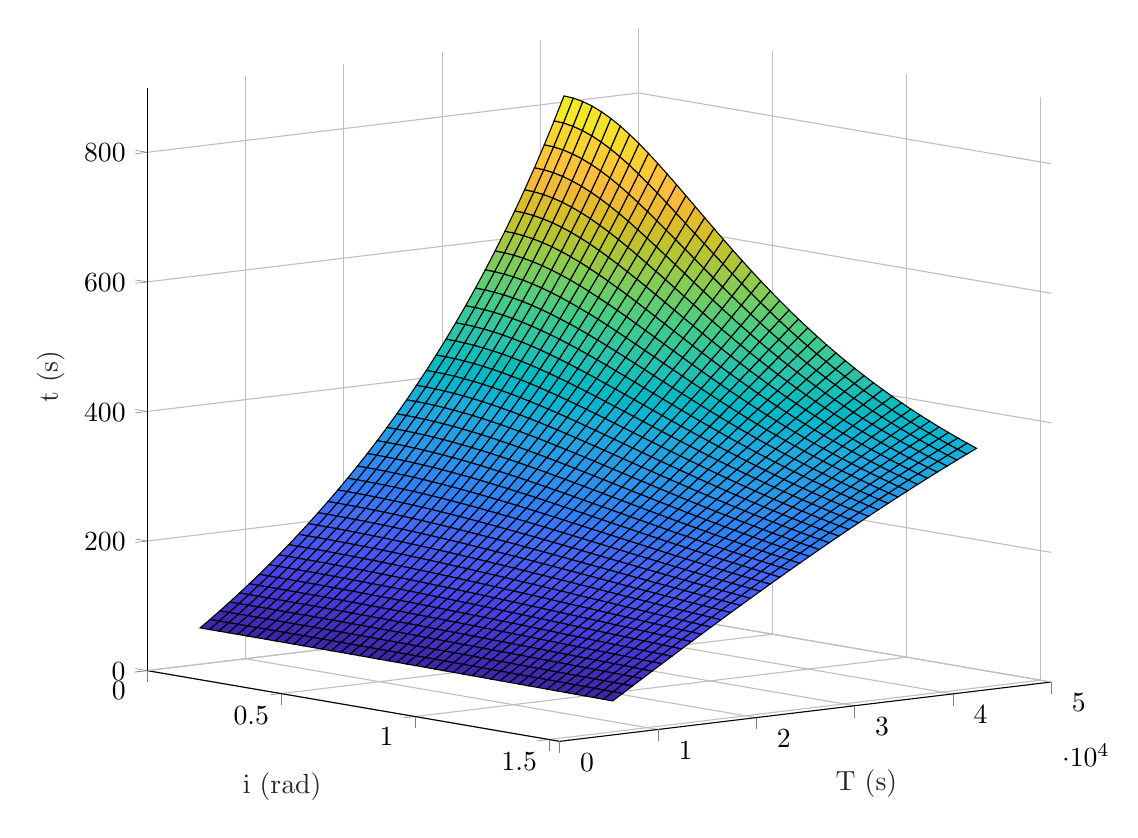
\begin{tikzpicture}

\begin{axis}[%
width=4.521in,
height=3.566in,
at={(0.758in,0.481in)},
scale only axis,
xmin=0,
xmax=1.54,
tick align=outside,
xlabel style={font=\color{white!15!black}},
xlabel={i (rad)},
ymin=0,
ymax=50000,
ylabel style={font=\color{white!15!black}},
ylabel={T (s)},
zmin=0,
zmax=900,
zlabel style={font=\color{white!15!black}},
zlabel={t (s)},
view={-310}{9},
axis background/.style={fill=white},
axis x line*=bottom,
axis y line*=left,
axis z line*=left,
xmajorgrids,
ymajorgrids,
zmajorgrids
]

\addplot3[%
surf,
shader=flat corner, draw=black, z buffer=sort, colormap={mymap}{[1pt] rgb(0pt)=(0.2422,0.1504,0.6603); rgb(1pt)=(0.2444,0.1534,0.6728); rgb(2pt)=(0.2464,0.1569,0.6847); rgb(3pt)=(0.2484,0.1607,0.6961); rgb(4pt)=(0.2503,0.1648,0.7071); rgb(5pt)=(0.2522,0.1689,0.7179); rgb(6pt)=(0.254,0.1732,0.7286); rgb(7pt)=(0.2558,0.1773,0.7393); rgb(8pt)=(0.2576,0.1814,0.7501); rgb(9pt)=(0.2594,0.1854,0.761); rgb(11pt)=(0.2628,0.1932,0.7828); rgb(12pt)=(0.2645,0.1972,0.7937); rgb(13pt)=(0.2661,0.2011,0.8043); rgb(14pt)=(0.2676,0.2052,0.8148); rgb(15pt)=(0.2691,0.2094,0.8249); rgb(16pt)=(0.2704,0.2138,0.8346); rgb(17pt)=(0.2717,0.2184,0.8439); rgb(18pt)=(0.2729,0.2231,0.8528); rgb(19pt)=(0.274,0.228,0.8612); rgb(20pt)=(0.2749,0.233,0.8692); rgb(21pt)=(0.2758,0.2382,0.8767); rgb(22pt)=(0.2766,0.2435,0.884); rgb(23pt)=(0.2774,0.2489,0.8908); rgb(24pt)=(0.2781,0.2543,0.8973); rgb(25pt)=(0.2788,0.2598,0.9035); rgb(26pt)=(0.2794,0.2653,0.9094); rgb(27pt)=(0.2798,0.2708,0.915); rgb(28pt)=(0.2802,0.2764,0.9204); rgb(29pt)=(0.2806,0.2819,0.9255); rgb(30pt)=(0.2809,0.2875,0.9305); rgb(31pt)=(0.2811,0.293,0.9352); rgb(32pt)=(0.2813,0.2985,0.9397); rgb(33pt)=(0.2814,0.304,0.9441); rgb(34pt)=(0.2814,0.3095,0.9483); rgb(35pt)=(0.2813,0.315,0.9524); rgb(36pt)=(0.2811,0.3204,0.9563); rgb(37pt)=(0.2809,0.3259,0.96); rgb(38pt)=(0.2807,0.3313,0.9636); rgb(39pt)=(0.2803,0.3367,0.967); rgb(40pt)=(0.2798,0.3421,0.9702); rgb(41pt)=(0.2791,0.3475,0.9733); rgb(42pt)=(0.2784,0.3529,0.9763); rgb(43pt)=(0.2776,0.3583,0.9791); rgb(44pt)=(0.2766,0.3638,0.9817); rgb(45pt)=(0.2754,0.3693,0.984); rgb(46pt)=(0.2741,0.3748,0.9862); rgb(47pt)=(0.2726,0.3804,0.9881); rgb(48pt)=(0.271,0.386,0.9898); rgb(49pt)=(0.2691,0.3916,0.9912); rgb(50pt)=(0.267,0.3973,0.9924); rgb(51pt)=(0.2647,0.403,0.9935); rgb(52pt)=(0.2621,0.4088,0.9946); rgb(53pt)=(0.2591,0.4145,0.9955); rgb(54pt)=(0.2556,0.4203,0.9965); rgb(55pt)=(0.2517,0.4261,0.9974); rgb(56pt)=(0.2473,0.4319,0.9983); rgb(57pt)=(0.2424,0.4378,0.9991); rgb(58pt)=(0.2369,0.4437,0.9996); rgb(59pt)=(0.2311,0.4497,0.9995); rgb(60pt)=(0.225,0.4559,0.9985); rgb(61pt)=(0.2189,0.462,0.9968); rgb(62pt)=(0.2128,0.4682,0.9948); rgb(63pt)=(0.2066,0.4743,0.9926); rgb(64pt)=(0.2006,0.4803,0.9906); rgb(65pt)=(0.195,0.4861,0.9887); rgb(66pt)=(0.1903,0.4919,0.9867); rgb(67pt)=(0.1869,0.4975,0.9844); rgb(68pt)=(0.1847,0.503,0.9819); rgb(69pt)=(0.1831,0.5084,0.9793); rgb(70pt)=(0.1818,0.5138,0.9766); rgb(71pt)=(0.1806,0.5191,0.9738); rgb(72pt)=(0.1795,0.5244,0.9709); rgb(73pt)=(0.1785,0.5296,0.9677); rgb(74pt)=(0.1778,0.5349,0.9641); rgb(75pt)=(0.1773,0.5401,0.9602); rgb(76pt)=(0.1768,0.5452,0.956); rgb(77pt)=(0.1764,0.5504,0.9516); rgb(78pt)=(0.1755,0.5554,0.9473); rgb(79pt)=(0.174,0.5605,0.9432); rgb(80pt)=(0.1716,0.5655,0.9393); rgb(81pt)=(0.1686,0.5705,0.9357); rgb(82pt)=(0.1649,0.5755,0.9323); rgb(83pt)=(0.161,0.5805,0.9289); rgb(84pt)=(0.1573,0.5854,0.9254); rgb(85pt)=(0.154,0.5902,0.9218); rgb(86pt)=(0.1513,0.595,0.9182); rgb(87pt)=(0.1492,0.5997,0.9147); rgb(88pt)=(0.1475,0.6043,0.9113); rgb(89pt)=(0.1461,0.6089,0.908); rgb(90pt)=(0.1446,0.6135,0.905); rgb(91pt)=(0.1429,0.618,0.9022); rgb(92pt)=(0.1408,0.6226,0.8998); rgb(93pt)=(0.1383,0.6272,0.8975); rgb(94pt)=(0.1354,0.6317,0.8953); rgb(95pt)=(0.1321,0.6363,0.8932); rgb(96pt)=(0.1288,0.6408,0.891); rgb(97pt)=(0.1253,0.6453,0.8887); rgb(98pt)=(0.1219,0.6497,0.8862); rgb(99pt)=(0.1185,0.6541,0.8834); rgb(100pt)=(0.1152,0.6584,0.8804); rgb(101pt)=(0.1119,0.6627,0.877); rgb(102pt)=(0.1085,0.6669,0.8734); rgb(103pt)=(0.1048,0.671,0.8695); rgb(104pt)=(0.1009,0.675,0.8653); rgb(105pt)=(0.0964,0.6789,0.8609); rgb(106pt)=(0.0914,0.6828,0.8562); rgb(107pt)=(0.0855,0.6865,0.8513); rgb(108pt)=(0.0789,0.6902,0.8462); rgb(109pt)=(0.0713,0.6938,0.8409); rgb(110pt)=(0.0628,0.6972,0.8355); rgb(111pt)=(0.0535,0.7006,0.8299); rgb(112pt)=(0.0433,0.7039,0.8242); rgb(113pt)=(0.0328,0.7071,0.8183); rgb(114pt)=(0.0234,0.7103,0.8124); rgb(115pt)=(0.0155,0.7133,0.8064); rgb(116pt)=(0.0091,0.7163,0.8003); rgb(117pt)=(0.0046,0.7192,0.7941); rgb(118pt)=(0.0019,0.722,0.7878); rgb(119pt)=(0.0009,0.7248,0.7815); rgb(120pt)=(0.0018,0.7275,0.7752); rgb(121pt)=(0.0046,0.7301,0.7688); rgb(122pt)=(0.0094,0.7327,0.7623); rgb(123pt)=(0.0162,0.7352,0.7558); rgb(124pt)=(0.0253,0.7376,0.7492); rgb(125pt)=(0.0369,0.74,0.7426); rgb(126pt)=(0.0504,0.7423,0.7359); rgb(127pt)=(0.0638,0.7446,0.7292); rgb(128pt)=(0.077,0.7468,0.7224); rgb(129pt)=(0.0899,0.7489,0.7156); rgb(130pt)=(0.1023,0.751,0.7088); rgb(131pt)=(0.1141,0.7531,0.7019); rgb(132pt)=(0.1252,0.7552,0.695); rgb(133pt)=(0.1354,0.7572,0.6881); rgb(134pt)=(0.1448,0.7593,0.6812); rgb(135pt)=(0.1532,0.7614,0.6741); rgb(136pt)=(0.1609,0.7635,0.6671); rgb(137pt)=(0.1678,0.7656,0.6599); rgb(138pt)=(0.1741,0.7678,0.6527); rgb(139pt)=(0.1799,0.7699,0.6454); rgb(140pt)=(0.1853,0.7721,0.6379); rgb(141pt)=(0.1905,0.7743,0.6303); rgb(142pt)=(0.1954,0.7765,0.6225); rgb(143pt)=(0.2003,0.7787,0.6146); rgb(144pt)=(0.2061,0.7808,0.6065); rgb(145pt)=(0.2118,0.7828,0.5983); rgb(146pt)=(0.2178,0.7849,0.5899); rgb(147pt)=(0.2244,0.7869,0.5813); rgb(148pt)=(0.2318,0.7887,0.5725); rgb(149pt)=(0.2401,0.7905,0.5636); rgb(150pt)=(0.2491,0.7922,0.5546); rgb(151pt)=(0.2589,0.7937,0.5454); rgb(152pt)=(0.2695,0.7951,0.536); rgb(153pt)=(0.2809,0.7964,0.5266); rgb(154pt)=(0.2929,0.7975,0.517); rgb(155pt)=(0.3052,0.7985,0.5074); rgb(156pt)=(0.3176,0.7994,0.4975); rgb(157pt)=(0.3301,0.8002,0.4876); rgb(158pt)=(0.3424,0.8009,0.4774); rgb(159pt)=(0.3548,0.8016,0.4669); rgb(160pt)=(0.3671,0.8021,0.4563); rgb(161pt)=(0.3795,0.8026,0.4454); rgb(162pt)=(0.3921,0.8029,0.4344); rgb(163pt)=(0.405,0.8031,0.4233); rgb(164pt)=(0.4184,0.803,0.4122); rgb(165pt)=(0.4322,0.8028,0.4013); rgb(166pt)=(0.4463,0.8024,0.3904); rgb(167pt)=(0.4608,0.8018,0.3797); rgb(168pt)=(0.4753,0.8011,0.3691); rgb(169pt)=(0.4899,0.8002,0.3586); rgb(170pt)=(0.5044,0.7993,0.348); rgb(171pt)=(0.5187,0.7982,0.3374); rgb(172pt)=(0.5329,0.797,0.3267); rgb(173pt)=(0.547,0.7957,0.3159); rgb(175pt)=(0.5748,0.7929,0.2941); rgb(176pt)=(0.5886,0.7913,0.2833); rgb(177pt)=(0.6024,0.7896,0.2726); rgb(178pt)=(0.6161,0.7878,0.2622); rgb(179pt)=(0.6297,0.7859,0.2521); rgb(180pt)=(0.6433,0.7839,0.2423); rgb(181pt)=(0.6567,0.7818,0.2329); rgb(182pt)=(0.6701,0.7796,0.2239); rgb(183pt)=(0.6833,0.7773,0.2155); rgb(184pt)=(0.6963,0.775,0.2075); rgb(185pt)=(0.7091,0.7727,0.1998); rgb(186pt)=(0.7218,0.7703,0.1924); rgb(187pt)=(0.7344,0.7679,0.1852); rgb(188pt)=(0.7468,0.7654,0.1782); rgb(189pt)=(0.759,0.7629,0.1717); rgb(190pt)=(0.771,0.7604,0.1658); rgb(191pt)=(0.7829,0.7579,0.1608); rgb(192pt)=(0.7945,0.7554,0.157); rgb(193pt)=(0.806,0.7529,0.1546); rgb(194pt)=(0.8172,0.7505,0.1535); rgb(195pt)=(0.8281,0.7481,0.1536); rgb(196pt)=(0.8389,0.7457,0.1546); rgb(197pt)=(0.8495,0.7435,0.1564); rgb(198pt)=(0.86,0.7413,0.1587); rgb(199pt)=(0.8703,0.7392,0.1615); rgb(200pt)=(0.8804,0.7372,0.165); rgb(201pt)=(0.8903,0.7353,0.1695); rgb(202pt)=(0.9,0.7336,0.1749); rgb(203pt)=(0.9093,0.7321,0.1815); rgb(204pt)=(0.9184,0.7308,0.189); rgb(205pt)=(0.9272,0.7298,0.1973); rgb(206pt)=(0.9357,0.729,0.2061); rgb(207pt)=(0.944,0.7285,0.2151); rgb(208pt)=(0.9523,0.7284,0.2237); rgb(209pt)=(0.9606,0.7285,0.2312); rgb(210pt)=(0.9689,0.7292,0.2373); rgb(211pt)=(0.977,0.7304,0.2418); rgb(212pt)=(0.9842,0.733,0.2446); rgb(213pt)=(0.99,0.7365,0.2429); rgb(214pt)=(0.9946,0.7407,0.2394); rgb(215pt)=(0.9966,0.7458,0.2351); rgb(216pt)=(0.9971,0.7513,0.2309); rgb(217pt)=(0.9972,0.7569,0.2267); rgb(218pt)=(0.9971,0.7626,0.2224); rgb(219pt)=(0.9969,0.7683,0.2181); rgb(220pt)=(0.9966,0.774,0.2138); rgb(221pt)=(0.9962,0.7798,0.2095); rgb(222pt)=(0.9957,0.7856,0.2053); rgb(223pt)=(0.9949,0.7915,0.2012); rgb(224pt)=(0.9938,0.7974,0.1974); rgb(225pt)=(0.9923,0.8034,0.1939); rgb(226pt)=(0.9906,0.8095,0.1906); rgb(227pt)=(0.9885,0.8156,0.1875); rgb(228pt)=(0.9861,0.8218,0.1846); rgb(229pt)=(0.9835,0.828,0.1817); rgb(230pt)=(0.9807,0.8342,0.1787); rgb(231pt)=(0.9778,0.8404,0.1757); rgb(232pt)=(0.9748,0.8467,0.1726); rgb(233pt)=(0.972,0.8529,0.1695); rgb(234pt)=(0.9694,0.8591,0.1665); rgb(235pt)=(0.9671,0.8654,0.1636); rgb(236pt)=(0.9651,0.8716,0.1608); rgb(237pt)=(0.9634,0.8778,0.1582); rgb(238pt)=(0.9619,0.884,0.1557); rgb(239pt)=(0.9608,0.8902,0.1532); rgb(240pt)=(0.9601,0.8963,0.1507); rgb(241pt)=(0.9596,0.9023,0.148); rgb(242pt)=(0.9595,0.9084,0.145); rgb(243pt)=(0.9597,0.9143,0.1418); rgb(244pt)=(0.9601,0.9203,0.1382); rgb(245pt)=(0.9608,0.9262,0.1344); rgb(246pt)=(0.9618,0.932,0.1304); rgb(247pt)=(0.9629,0.9379,0.1261); rgb(248pt)=(0.9642,0.9437,0.1216); rgb(249pt)=(0.9657,0.9494,0.1168); rgb(250pt)=(0.9674,0.9552,0.1116); rgb(251pt)=(0.9692,0.9609,0.1061); rgb(252pt)=(0.9711,0.9667,0.1001); rgb(253pt)=(0.973,0.9724,0.0938); rgb(254pt)=(0.9749,0.9782,0.0872); rgb(255pt)=(0.9769,0.9839,0.0805)}, mesh/rows=45]
table[row sep=crcr, point meta=\thisrow{c}] {%
%
x	y	z	c\\
0	5400	56	56\\
0	6400	67.2	67.2\\
0	7400	78.6835443037975	78.6835443037975\\
0	8400	90.4615384615385	90.4615384615385\\
0	9400	102.545454545455	102.545454545455\\
0	10400	114.947368421053	114.947368421053\\
0	11400	127.68	127.68\\
0	12400	140.756756756757	140.756756756757\\
0	13400	154.191780821918	154.191780821918\\
0	14400	168	168\\
0	15400	182.197183098592	182.197183098592\\
0	16400	196.8	196.8\\
0	17400	211.826086956522	211.826086956522\\
0	18400	227.294117647059	227.294117647059\\
0	19400	243.223880597015	243.223880597015\\
0	20400	259.636363636364	259.636363636364\\
0	21400	276.553846153846	276.553846153846\\
0	22400	294	294\\
0	23400	312	312\\
0	24400	330.58064516129	330.58064516129\\
0	25400	349.770491803279	349.770491803279\\
0	26400	369.6	369.6\\
0	27400	390.101694915254	390.101694915254\\
0	28400	411.310344827586	411.310344827586\\
0	29400	433.263157894737	433.263157894737\\
0	30400	456	456\\
0	31400	479.563636363636	479.563636363636\\
0	32400	504	504\\
0	33400	529.358490566038	529.358490566038\\
0	34400	555.692307692308	555.692307692308\\
0	35400	583.058823529412	583.058823529412\\
0	36400	611.52	611.52\\
0	37400	641.142857142857	641.142857142857\\
0	38400	672	672\\
0	39400	704.170212765958	704.170212765958\\
0	40400	737.739130434783	737.739130434783\\
0	41400	772.8	772.8\\
0	42400	809.454545454546	809.454545454546\\
0.035	5400	55.9975612971825	55.9975612971825\\
0.035	6400	67.1964444212269	67.1964444212269\\
0.035	7400	78.6786080658929	78.6786080658929\\
0.035	8400	90.4549302800604	90.4549302800604\\
0.035	9400	102.536852857731	102.536852857731\\
0.035	10400	114.93641830738	114.93641830738\\
0.035	11400	127.666309766816	127.666309766816\\
0.035	12400	140.739894140764	140.739894140764\\
0.035	13400	154.171268768654	154.171268768654\\
0.035	14400	167.97531196397	167.97531196397\\
0.035	15400	182.167737804823	182.167737804823\\
0.035	16400	196.765155598438	196.765155598438\\
0.035	17400	211.785134490994	211.785134490994\\
0.035	18400	227.24627374928	227.24627374928\\
0.035	19400	243.168279303091	243.168279303091\\
0.035	20400	259.572047208099	259.572047208099\\
0.035	21400	276.479754769559	276.479754769559\\
0.035	22400	293.914960158995	293.914960158995\\
0.035	23400	311.902711460816	311.902711460816\\
0.035	24400	330.469666205732	330.469666205732\\
0.035	25400	349.64422258516	349.64422258516\\
0.035	26400	369.456663698677	369.456663698677\\
0.035	27400	389.939316368122	389.939316368122\\
0.035	28400	411.126726261444	411.126726261444\\
0.035	29400	433.055851311588	433.055851311588\\
0.035	30400	455.766275696301	455.766275696301\\
0.035	31400	479.300446970774	479.300446970774\\
0.035	32400	503.703939324655	503.703939324655\\
0.035	33400	529.025746378203	529.025746378203\\
0.035	34400	555.318607451279	555.318607451279\\
0.035	35400	582.639371848002	582.639371848002\\
0.035	36400	611.049406417077	611.049406417077\\
0.035	37400	640.615052494642	640.615052494642\\
0.035	38400	671.408139339471	671.408139339471\\
0.035	39400	703.50656236223	703.50656236223\\
0.035	40400	736.994935871291	736.994935871291\\
0.035	41400	771.965331757367	771.965331757367\\
0.035	42400	808.518117579786	808.518117579786\\
0.07	5400	55.9902500856498	55.9902500856498\\
0.07	6400	67.1857854229613	67.1857854229613\\
0.07	7400	78.6638109667858	78.6638109667858\\
0.07	8400	90.4351225092879	90.4351225092879\\
0.07	9400	102.511071302908	102.511071302908\\
0.07	10400	114.903600132277	114.903600132277\\
0.07	11400	127.62528222447	127.62528222447\\
0.07	12400	140.689363260666	140.689363260666\\
0.07	13400	154.109806780432	154.109806780432\\
0.07	14400	167.901343301379	167.901343301379\\
0.07	15400	182.079523512399	182.079523512399\\
0.07	16400	196.6607759385	196.6607759385\\
0.07	17400	211.662469520195	211.662469520195\\
0.07	18400	227.102981600988	227.102981600988\\
0.07	19400	243.001771873729	243.001771873729\\
0.07	20400	259.379462901368	259.379462901368\\
0.07	21400	276.257927900991	276.257927900991\\
0.07	22400	293.660386563375	293.660386563375\\
0.07	23400	311.611509775064	311.611509775064\\
0.07	24400	330.13753421795	330.13753421795\\
0.07	25400	349.266387944626	349.266387944626\\
0.07	26400	369.027828168733	369.027828168733\\
0.07	27400	389.453592671063	389.453592671063\\
0.07	28400	410.577566407613	410.577566407613\\
0.07	29400	432.435965119123	432.435965119123\\
0.07	30400	455.067537987527	455.067537987527\\
0.07	31400	478.51379166887	478.51379166887\\
0.07	32400	502.819238361074	502.819238361074\\
0.07	33400	528.031670946632	528.031670946632\\
0.07	34400	554.202468694044	554.202468694044\\
0.07	35400	581.386937519266	581.386937519266\\
0.07	36400	609.644689412965	609.644689412965\\
0.07	37400	639.040066347644	639.040066347644\\
0.07	38400	669.642614810532	669.642614810532\\
0.07	39400	701.527618087564	701.527618087564\\
0.07	40400	734.776694580318	734.776694580318\\
0.07	41400	769.478471806897	769.478471806897\\
0.07	42400	805.729347363441	805.729347363441\\
0.105	5400	55.978081036663	55.978081036663\\
0.105	6400	67.1680461843939	67.1680461843939\\
0.105	7400	78.6391877913849	78.6391877913849\\
0.105	8400	90.402165375552	90.402165375552\\
0.105	9400	102.468180259482	102.468180259482\\
0.105	10400	114.849010173229	114.849010173229\\
0.105	11400	127.557046521536	127.557046521536\\
0.105	12400	140.605334555809	140.605334555809\\
0.105	13400	154.007616716012	154.007616716012\\
0.105	14400	167.778379435435	167.778379435435\\
0.105	15400	181.932903732259	181.932903732259\\
0.105	16400	196.487319946619	196.487319946619\\
0.105	17400	211.458667020737	211.458667020737\\
0.105	18400	226.864956763402	226.864956763402\\
0.105	19400	242.725243589115	242.725243589115\\
0.105	20400	259.059700277442	259.059700277442\\
0.105	21400	275.8897003603	275.8897003603\\
0.105	22400	293.237907815076	293.237907815076\\
0.105	23400	311.128374820741	311.128374820741\\
0.105	24400	329.586648423768	329.586648423768\\
0.105	25400	348.639887062281	348.639887062281\\
0.105	26400	368.31698801207	368.31698801207\\
0.105	27400	388.648726949036	388.648726949036\\
0.105	28400	409.667910971607	409.667910971607\\
0.105	29400	431.409546596356	431.409546596356\\
0.105	30400	453.911024433757	453.911024433757\\
0.105	31400	477.212322472291	477.212322472291\\
0.105	32400	501.356230152414	501.356230152414\\
0.105	33400	526.388595702141	526.388595702141\\
0.105	34400	552.358599539165	552.358599539165\\
0.105	35400	579.319056927311	579.319056927311\\
0.105	36400	607.32675351579	607.32675351579\\
0.105	37400	636.442817897573	636.442817897573\\
0.105	38400	666.733135909187	666.733135909187\\
0.105	39400	698.26881207119	698.26881207119\\
0.105	40400	731.126684351446	731.126684351446\\
0.105	41400	765.38989933953	765.38989933953\\
0.105	42400	801.148555970364	801.148555970364\\
0.14	5400	55.9610785374807	55.9610785374807\\
0.14	6400	67.1432652212536	67.1432652212536\\
0.14	7400	78.6047963187556	78.6047963187556\\
0.14	8400	90.3561422749416	90.3561422749416\\
0.14	9400	102.408296538235	102.408296538235\\
0.14	10400	114.772808161498	114.772808161498\\
0.14	11400	127.461816833561	127.461816833561\\
0.14	12400	140.488090551553	140.488090551553\\
0.14	13400	153.865066164841	153.865066164841\\
0.14	14400	167.606893044258	167.606893044258\\
0.14	15400	181.728480155603	181.728480155603\\
0.14	16400	196.245546844568	196.245546844568\\
0.14	17400	211.174677671484	211.174677671484\\
0.14	18400	226.533381669108	226.533381669108\\
0.14	19400	242.340156435364	242.340156435364\\
0.14	20400	258.614557516123	258.614557516123\\
0.14	21400	275.377273581188	275.377273581188\\
0.14	22400	292.650207950336	292.650207950336\\
0.14	23400	310.456567086161	310.456567086161\\
0.14	24400	328.820956737413	328.820956737413\\
0.14	25400	347.769486491317	347.769486491317\\
0.14	26400	367.329883577031	367.329883577031\\
0.14	27400	387.531616855953	387.531616855953\\
0.14	28400	408.406032039352	408.406032039352\\
0.14	29400	429.986499290957	429.986499290957\\
0.14	30400	452.308574503359	452.308574503359\\
0.14	31400	475.41017568386	475.41017568386\\
0.14	32400	499.33177604962	499.33177604962\\
0.14	33400	524.116615615569	524.116615615569\\
0.14	34400	549.810933263572	549.810933263572\\
0.14	35400	576.464221510101	576.464221510101\\
0.14	36400	604.129506444303	604.129506444303\\
0.14	37400	632.863655591267	632.863655591267\\
0.14	38400	662.727716768475	662.727716768475\\
0.14	39400	693.787291348845	693.787291348845\\
0.14	40400	726.112945722563	726.112945722563\\
0.14	41400	759.780665162457	759.780665162457\\
0.14	42400	794.872354742718	794.872354742718\\
0.175	5400	55.9392765946292	55.9392765946292\\
0.175	6400	67.1114962125119	67.1114962125119\\
0.175	7400	78.5607170304984	78.5607170304984\\
0.175	8400	90.2971693052713	90.2971693052713\\
0.175	9400	102.331582658423	102.331582658423\\
0.175	10400	114.675216195595	114.675216195595\\
0.175	11400	127.339890771425	127.339890771425\\
0.175	12400	140.338023574689	140.338023574689\\
0.175	13400	153.682665223722	153.682665223722\\
0.175	14400	167.387539579316	167.387539579316\\
0.175	15400	181.467086501166	181.467086501166\\
0.175	16400	195.936507794495	195.936507794495\\
0.175	17400	210.811816616121	210.811816616121\\
0.175	18400	226.109890633938	226.109890633938\\
0.175	19400	241.848529260918	241.848529260918\\
0.175	20400	258.046515314365	258.046515314365\\
0.175	21400	274.723681483632	274.723681483632\\
0.175	22400	291.90098202493	291.90098202493\\
0.175	23400	309.6005701406	309.6005701406\\
0.175	24400	327.845881542345	327.845881542345\\
0.175	25400	346.66172474387	346.66172474387\\
0.175	26400	366.074378678136	366.074378678136\\
0.175	27400	386.111698288377	386.111698288377\\
0.175	28400	406.803228800178	406.803228800178\\
0.175	29400	428.18032944434	428.18032944434\\
0.175	30400	450.276307466969	450.276307466969\\
0.175	31400	473.126563333927	473.126563333927\\
0.175	32400	496.768748111155	496.768748111155\\
0.175	33400	521.242934079586	521.242934079586\\
0.175	34400	546.591799722454	546.591799722454\\
0.175	35400	572.860830301919	572.860830301919\\
0.175	36400	600.0985353189	600.0985353189\\
0.175	37400	628.356684221351	628.356684221351\\
0.175	38400	657.690561787405	657.690561787405\\
0.175	39400	688.159244654548	688.159244654548\\
0.175	40400	719.825900485765	719.825900485765\\
0.175	41400	752.758111247094	752.758111247094\\
0.175	42400	787.028222002904	787.028222002904\\
0.21	5400	55.9127186995428	55.9127186995428\\
0.21	6400	67.0728077599265	67.0728077599265\\
0.21	7400	78.5070527065501	78.5070527065501\\
0.21	8400	90.2253946180906	90.2253946180906\\
0.21	9400	102.238245846803	102.238245846803\\
0.21	10400	114.556517240507	114.556517240507\\
0.21	11400	127.191647185601	127.191647185601\\
0.21	12400	140.155632605815	140.155632605815\\
0.21	13400	153.461062061811	153.461062061811\\
0.21	14400	167.121151107901	167.121151107901\\
0.21	15400	181.149780074066	181.149780074066\\
0.21	16400	195.561534454195	195.561534454195\\
0.21	17400	210.371748095012	210.371748095012\\
0.21	18400	225.596549394508	225.596549394508\\
0.21	19400	241.252910733879	241.252910733879\\
0.21	20400	257.358701382909	257.358701382909\\
0.21	21400	273.932744135347	273.932744135347\\
0.21	22400	290.994875948102	290.994875948102\\
0.21	23400	308.566012875714	308.566012875714\\
0.21	24400	326.668219609468	326.668219609468\\
0.21	25400	345.324783948328	345.324783948328\\
0.21	26400	364.560296546173	364.560296546173\\
0.21	27400	384.400736296072	384.400736296072\\
0.21	28400	404.873561726888	404.873561726888\\
0.21	29400	426.007808799284	426.007808799284\\
0.21	30400	447.834195496167	447.834195496167\\
0.21	31400	470.385233605069	470.385233605069\\
0.21	32400	493.695348085042	493.695348085042\\
0.21	33400	517.801004395743	517.801004395743\\
0.21	34400	542.740844138308	542.740844138308\\
0.21	35400	568.555829312377	568.555829312377\\
0.21	36400	595.289395425935	595.289395425935\\
0.21	37400	622.987613598217	622.987613598217\\
0.21	38400	651.69936166248	651.69936166248\\
0.21	39400	681.476504094854	681.476504094854\\
0.21	40400	712.374080354973	712.374080354973\\
0.21	41400	744.450500907594	744.450500907594\\
0.21	42400	777.767749782096	777.767749782096\\
0.245	5400	55.8814576576189	55.8814576576189\\
0.245	6400	67.0272830825455	67.0272830825455\\
0.245	7400	78.4439279123955	78.4439279123955\\
0.245	8400	90.140997597831	90.140997597831\\
0.245	9400	102.128536771585	102.128536771585\\
0.245	10400	114.417053232492	114.417053232492\\
0.245	11400	127.017543397931	127.017543397931\\
0.245	12400	139.941519317881	139.941519317881\\
0.245	13400	153.201037348964	153.201037348964\\
0.245	14400	166.80872859204	166.80872859204\\
0.245	15400	180.777831202085	180.777831202085\\
0.245	16400	195.122224684163	195.122224684163\\
0.245	17400	209.856466294097	209.856466294097\\
0.245	18400	224.995829666928	224.995829666928\\
0.245	19400	240.556345800111	240.556345800111\\
0.245	20400	256.554846521534	256.554846521534\\
0.245	21400	273.009010574413	273.009010574413\\
0.245	22400	289.937412451758	289.937412451758\\
0.245	23400	307.359574111775	307.359574111775\\
0.245	24400	325.296019701859	325.296019701859\\
0.245	25400	343.768333412033	343.768333412033\\
0.245	26400	362.799220567944	362.799220567944\\
0.245	27400	382.412572057867	382.412572057867\\
0.245	28400	402.633532166335	402.633532166335\\
0.245	29400	423.488569857517	423.488569857517\\
0.245	30400	445.005553512414	445.005553512414\\
0.245	31400	467.213829073194	467.213829073194\\
0.245	32400	490.144301482674	490.144301482674\\
0.245	33400	513.82951922394	513.82951922394\\
0.245	34400	538.303761660226	538.303761660226\\
0.245	35400	563.603128743681	563.603128743681\\
0.245	36400	589.765632497729	589.765632497729\\
0.245	37400	616.831289474208	616.831289474208\\
0.245	38400	644.84221313509	644.84221313509\\
0.245	39400	673.842704799033	673.842704799033\\
0.245	40400	703.879341413388	703.879341413388\\
0.245	41400	735.001057948113	735.001057948113\\
0.245	42400	767.259221642454	767.259221642454\\
0.28	5400	55.8455553820094	55.8455553820094\\
0.28	6400	66.9750196488442	66.9750196488442\\
0.28	7400	78.3714883827108	78.3714883827108\\
0.28	8400	90.0441878769939	90.0441878769939\\
0.28	9400	102.002748026407	102.002748026407\\
0.28	10400	114.257222814203	114.257222814203\\
0.28	11400	126.818111900253	126.818111900253\\
0.28	12400	139.696383361968	139.696383361968\\
0.28	13400	152.903497640263	152.903497640263\\
0.28	14400	166.45143274249	166.45143274249\\
0.28	15400	180.352710753276	180.352710753276\\
0.28	16400	194.62042570231	194.62042570231\\
0.28	17400	209.268272835192	209.268272835192\\
0.28	18400	224.310579329156	224.310579329156\\
0.28	19400	239.762336489595	239.762336489595\\
0.28	20400	255.639233455408	255.639233455408\\
0.28	21400	271.957692430912	271.957692430912\\
0.28	22400	288.734905448842	288.734905448842\\
0.28	23400	305.988872652301	305.988872652301\\
0.28	24400	323.738442062529	323.738442062529\\
0.28	25400	342.003350773419	342.003350773419\\
0.28	26400	360.804267481633	360.804267481633\\
0.28	27400	380.162836221817	380.162836221817\\
0.28	28400	400.101721128474	400.101721128474\\
0.28	29400	420.644651987735	420.644651987735\\
0.28	30400	441.816470271693	441.816470271693\\
0.28	31400	463.643175262884	463.643175262884\\
0.28	32400	486.1519697741	486.1519697741\\
0.28	33400	509.371304846035	509.371304846035\\
0.28	34400	533.330922658482	533.330922658482\\
0.28	35400	558.061896715804	558.061896715804\\
0.28	36400	583.596668159249	583.596668159249\\
0.28	37400	609.969076811732	609.969076811732\\
0.28	38400	637.214385268634	637.214385268634\\
0.28	39400	665.369294003648	665.369294003648\\
0.28	40400	694.471945053656	694.471945053656\\
0.28	41400	724.561911372129	724.561911372129\\
0.28	42400	755.680168386739	755.680168386739\\
0.315	5400	55.8050826537284	55.8050826537284\\
0.315	6400	66.9161287496827	66.9161287496827\\
0.315	7400	78.2899003074018	78.2899003074018\\
0.315	8400	89.93520419793	89.93520419793\\
0.315	9400	101.861212382194	101.861212382194\\
0.315	10400	114.077478729252	114.077478729252\\
0.315	11400	126.593956566066	126.593956566066\\
0.315	12400	139.421016971696	139.421016971696\\
0.315	13400	152.569467824839	152.569467824839\\
0.315	14400	166.050573608629	166.050573608629\\
0.315	15400	179.876075970423	179.876075970423\\
0.315	16400	194.058215026661	194.058215026661\\
0.315	17400	208.609751393592	208.609751393592\\
0.315	18400	223.543988913392	223.543988913392\\
0.315	19400	238.874798031601	238.874798031601\\
0.315	20400	254.616639765468	254.616639765468\\
0.315	21400	270.784590183321	270.784590183321\\
0.315	22400	287.394365291804	287.394365291804\\
0.315	23400	304.462346200218	304.462346200218\\
0.315	24400	322.005604398538	322.005604398538\\
0.315	25400	340.041926947028	340.041926947028\\
0.315	26400	358.589841329905	358.589841329905\\
0.315	27400	377.668639672002	377.668639672002\\
0.315	28400	397.298401954657	397.298401954657\\
0.315	29400	417.500017793645	417.500017793645\\
0.315	30400	438.295206256242	438.295206256242\\
0.315	31400	459.706533094635	459.706533094635\\
0.315	32400	481.757424656848	481.757424656848\\
0.315	33400	504.472177601739	504.472177601739\\
0.315	34400	527.875963389036	527.875963389036\\
0.315	35400	551.994826335983	551.994826335983\\
0.315	36400	576.85567382597	576.85567382597\\
0.315	37400	602.486257018444	602.486257018444\\
0.315	38400	628.915140140119	628.915140140119\\
0.315	39400	656.17165613186	656.17165613186\\
0.315	40400	684.28584608041	684.28584608041\\
0.315	41400	713.288379476866	713.288379476866\\
0.315	42400	743.210451912264	743.210451912264\\
0.35	5400	55.7601188498946	55.7601188498946\\
0.35	6400	66.8507350157404	66.8507350157404\\
0.35	7400	78.1993495268593	78.1993495268593\\
0.35	8400	89.8143131332262	89.8143131332262\\
0.35	9400	101.704300827126	101.704300827126\\
0.35	10400	113.878324909144	113.878324909144\\
0.35	11400	126.345748427172	126.345748427172\\
0.35	12400	139.116298966225	139.116298966225\\
0.35	13400	152.200082759535	152.200082759535\\
0.35	14400	165.607599082678	165.607599082678\\
0.35	15400	179.349754882381	179.349754882381\\
0.35	16400	193.437879579704	193.437879579704\\
0.35	17400	207.883739973449	207.883739973449\\
0.35	18400	222.699555153451	222.699555153451\\
0.35	19400	237.898011314624	237.898011314624\\
0.35	20400	253.49227634083	253.49227634083\\
0.35	21400	269.496014002416	269.496014002416\\
0.35	22400	285.923397582117	285.923397582117\\
0.35	23400	302.789122710379	302.789122710379\\
0.35	24400	320.108419152537	320.108419152537\\
0.35	25400	337.897061245776	337.897061245776\\
0.35	26400	356.171376632915	356.171376632915\\
0.35	27400	374.948252881784	374.948252881784\\
0.35	28400	394.245141512456	394.245141512456\\
0.35	29400	414.080058878939	414.080058878939\\
0.35	30400	434.471583265942	434.471583265942\\
0.35	31400	455.438847464106	455.438847464106\\
0.35	32400	477.001525977286	477.001525977286\\
0.35	33400	499.17981589211	499.17981589211\\
0.35	34400	521.994410301925	521.994410301925\\
0.35	35400	545.466463023378	545.466463023378\\
0.35	36400	569.617543173447	569.617543173447\\
0.35	37400	594.469577987087	594.469577987087\\
0.35	38400	620.044782050722	620.044782050722\\
0.35	39400	646.365570904996	646.365570904996\\
0.35	40400	673.454456732643	673.454456732643\\
0.35	41400	701.333923596643	701.333923596643\\
0.35	42400	730.026279433484	730.026279433484\\
0.385	5400	55.7107516421428	55.7107516421428\\
0.385	6400	66.7789758835011	66.7789758835011\\
0.385	7400	78.1000406439963	78.1000406439963\\
0.385	8400	89.6818076779747	89.6818076779747\\
0.385	9400	101.532420417015	101.532420417015\\
0.385	10400	113.660313288598	113.660313288598\\
0.385	11400	126.074221071854	126.074221071854\\
0.385	12400	138.78318823849	138.78318823849\\
0.385	13400	151.796578217288	151.796578217288\\
0.385	14400	165.124082509424	165.124082509424\\
0.385	15400	178.775729569134	178.775729569134\\
0.385	16400	192.761893349728	192.761893349728\\
0.385	17400	207.093301398385	207.093301398385\\
0.385	18400	221.781042364354	221.781042364354\\
0.385	19400	236.836572763766	236.836572763766\\
0.385	20400	252.271722820034	252.271722820034\\
0.385	21400	268.098701171396	268.098701171396\\
0.385	22400	284.330098206144	284.330098206144\\
0.385	23400	300.978887751204	300.978887751204\\
0.385	24400	318.05842680046	318.05842680046\\
0.385	25400	335.582452925223	335.582452925223\\
0.385	26400	353.565078959994	353.565078959994\\
0.385	27400	372.020784501819	372.020784501819\\
0.385	28400	390.9644037005	390.9644037005\\
0.385	29400	410.411108749466	410.411108749466\\
0.385	30400	430.376388412676	430.376388412676\\
0.385	31400	450.87602084132	450.87602084132\\
0.385	32400	471.92603984514	471.92603984514\\
0.385	33400	493.542693686795	493.542693686795\\
0.385	34400	515.742395364158	515.742395364158\\
0.385	35400	538.541663235176	538.541663235176\\
0.385	36400	561.957050723915	561.957050723915\\
0.385	37400	586.005063726039	586.005063726039\\
0.385	38400	610.702064209321	610.702064209321\\
0.385	39400	636.064158382711	636.064158382711\\
0.385	40400	662.107067689952	662.107067689952\\
0.385	41400	688.845980775778	688.845980775778\\
0.385	42400	716.295384481017	716.295384481017\\
0.42	5400	55.6570766674334	55.6570766674334\\
0.42	6400	66.7010010142282	66.7010010142282\\
0.42	7400	77.9921960612686	77.9921960612686\\
0.42	8400	89.5380057282349	89.5380057282349\\
0.42	9400	101.346011959939	101.346011959939\\
0.42	10400	113.424040387674	113.424040387674\\
0.42	11400	125.780165724592	125.780165724592\\
0.42	12400	138.422716819974	138.422716819974\\
0.42	13400	151.360281286248	151.360281286248\\
0.42	14400	164.601709600275	164.601709600275\\
0.42	15400	178.156118566537	178.156118566537\\
0.42	16400	192.032894014398	192.032894014398\\
0.42	17400	206.241692584224	206.241692584224\\
0.42	18400	220.792442437875	220.792442437875\\
0.42	19400	235.695342707517	235.695342707517\\
0.42	20400	250.960861472858	250.960861472858\\
0.42	21400	266.599732030457	266.599732030457\\
0.42	22400	282.622947189539	282.622947189539\\
0.42	23400	299.041751296605	299.041751296605\\
0.42	24400	315.867629655866	315.867629655866\\
0.42	25400	333.112294973984	333.112294973984\\
0.42	26400	350.787670415684	350.787670415684\\
0.42	27400	368.905868811456	368.905868811456\\
0.42	28400	387.479167509739	387.479167509739\\
0.42	29400	406.519978313869	406.519978313869\\
0.42	30400	426.040811888784	426.040811888784\\
0.42	31400	446.054235964527	446.054235964527\\
0.42	32400	466.572826603419	466.572826603419\\
0.42	33400	487.609111736324	487.609111736324\\
0.42	34400	509.175506111805	509.175506111805\\
0.42	35400	531.284236741616	531.284236741616\\
0.42	36400	553.947257869032	553.947257869032\\
0.42	37400	577.176154435284	577.176154435284\\
0.42	38400	600.982032977137	600.982032977137\\
0.42	39400	625.375398859226	625.375398859226\\
0.42	40400	650.366018732858	650.366018732858\\
0.42	41400	675.962767124248	675.962767124248\\
0.42	42400	702.173456096224	702.173456096224\\
0.455	5400	55.5991971736494	55.5991971736494\\
0.455	6400	66.6169716706676	66.6169716706676\\
0.455	7400	77.8760549513894	77.8760549513894\\
0.455	8400	89.3832484608036	89.3832484608036\\
0.455	9400	101.145547560218	101.145547560218\\
0.455	10400	113.170143700789	113.170143700789\\
0.455	11400	125.464426069458	125.464426069458\\
0.455	12400	138.03598261598	138.03598261598\\
0.455	13400	150.892600358554	150.892600358554\\
0.455	14400	164.042264853165	164.042264853165\\
0.455	15400	177.493158698125	177.493158698125\\
0.455	16400	191.253658930342	191.253658930342\\
0.455	17400	205.332333153449	205.332333153449\\
0.455	18400	219.737934220005	219.737934220005\\
0.455	19400	234.479393270477	234.479393270477\\
0.455	20400	249.565810910566	249.565810910566\\
0.455	21400	265.006446285546	265.006446285546\\
0.455	22400	280.810703785724	280.810703785724\\
0.455	23400	296.988117090779	296.988117090779\\
0.455	24400	313.548330232792	313.548330232792\\
0.455	25400	330.501075328193	330.501075328193\\
0.455	26400	347.85614659794	347.85614659794\\
0.455	27400	365.623370263158	365.623370263158\\
0.455	28400	383.812569870623	383.812569870623\\
0.455	29400	402.433526569353	402.433526569353\\
0.455	30400	421.4959338268	421.4959338268\\
0.455	31400	441.009346041586	441.009346041586\\
0.455	32400	460.983120480359	460.983120480359\\
0.455	33400	481.426351940584	481.426351940584\\
0.455	34400	502.347799520362	502.347799520362\\
0.455	35400	523.755804862753	523.755804862753\\
0.455	36400	545.658201237756	545.658201237756\\
0.455	37400	568.062212832806	568.062212832806\\
0.455	38400	590.974343645563	590.974343645563\\
0.455	39400	614.400255414407	614.400255414407\\
0.455	40400	638.344634086653	638.344634086653\\
0.455	41400	662.811044416459	662.811044416459\\
0.455	42400	687.801772408814	687.801772408814\\
0.49	5400	55.5372236425111	55.5372236425111\\
0.49	6400	66.5270600564618	66.5270600564618\\
0.49	7400	77.7518721708328	77.7518721708328\\
0.49	8400	89.217898629974	89.217898629974\\
0.49	9400	100.93152804755	100.93152804755\\
0.49	10400	112.899297933611	112.899297933611\\
0.49	11400	125.127892880297	125.127892880297\\
0.49	12400	137.624141906021	137.624141906021\\
0.49	13400	150.395014847511	150.395014847511\\
0.49	14400	163.447617677772	163.447617677772\\
0.49	15400	176.789186615774	176.789186615774\\
0.49	16400	190.427080880572	190.427080880572\\
0.49	17400	204.368773928476	204.368773928476\\
0.49	18400	218.621842996938	218.621842996938\\
0.49	19400	233.193956762927	233.193956762927\\
0.49	20400	248.092860906905	248.092860906905\\
0.49	21400	263.32636135601	263.32636135601\\
0.49	22400	278.902304961994	278.902304961994\\
0.49	23400	294.828557350916	294.828557350916\\
0.49	24400	311.112977662761	311.112977662761\\
0.49	25400	327.76338988048	327.76338988048\\
0.49	26400	344.787550429611	344.787550429611\\
0.49	27400	362.19311171227	362.19311171227\\
0.49	28400	379.987581223384	379.987581223384\\
0.49	29400	398.178275883325	398.178275883325\\
0.49	30400	416.772271210421	416.772271210421\\
0.49	31400	435.776344950176	435.776344950176\\
0.49	32400	455.196914776615	455.196914776615\\
0.49	33400	475.039969686387	475.039969686387\\
0.49	34400	495.310994719624	495.310994719624\\
0.49	35400	516.014888664951	516.014888664951\\
0.49	36400	537.155874441429	537.155874441429\\
0.49	37400	558.73740189987	558.73740189987\\
0.49	38400	580.762042852288	580.762042852288\\
0.49	39400	603.231378223827	603.231378223827\\
0.49	40400	626.145877329123	626.145877329123\\
0.49	41400	649.504769407304	649.504769407304\\
0.49	42400	673.305907709565	673.305907709565\\
0.525	5400	55.4712733924448	55.4712733924448\\
0.525	6400	66.431448623432	66.431448623432\\
0.525	7400	77.6199171254827	77.6199171254827\\
0.525	8400	89.0423387972879	89.0423387972879\\
0.525	9400	100.704480317479	100.704480317479\\
0.525	10400	112.612211129023	112.612211129023\\
0.525	11400	124.771498520554	124.771498520554\\
0.525	12400	137.188401702739	137.188401702739\\
0.525	13400	149.869064768812	149.869064768812\\
0.525	14400	162.819708419028	162.819708419028\\
0.525	15400	176.046620318833	176.046620318833\\
0.525	16400	189.556143950242	189.556143950242\\
0.525	17400	203.354665805176	203.354665805176\\
0.525	18400	217.448600758553	217.448600758553\\
0.525	19400	231.844375447705	231.844375447705\\
0.525	20400	246.54840947353	246.54840947353\\
0.525	21400	261.567094227719	261.567094227719\\
0.525	22400	276.906769139699	276.906769139699\\
0.525	23400	292.573695126954	292.573695126954\\
0.525	24400	308.574025023285	308.574025023285\\
0.525	25400	324.913770751979	324.913770751979\\
0.525	26400	341.598767005017	341.598767005017\\
0.525	27400	358.634631186105	358.634631186105\\
0.525	28400	376.026719375018	376.026719375018\\
0.525	29400	393.780078074206	393.780078074206\\
0.525	30400	411.89939150682	411.89939150682\\
0.525	31400	430.388924249052	430.388924249052\\
0.525	32400	449.252459000111	449.252459000111\\
0.525	33400	468.49322932144	468.49322932144\\
0.525	34400	488.113847214117	488.113847214117\\
0.525	35400	508.116225451173	508.116225451173\\
0.525	36400	528.501494641175	528.501494641175\\
0.525	37400	549.269915072297	549.269915072297\\
0.525	38400	570.420783473641	570.420783473641\\
0.525	39400	591.952334934036	591.952334934036\\
0.525	40400	613.861640339227	613.861640339227\\
0.525	41400	636.144499827005	636.144499827005\\
0.525	42400	658.795332917114	658.795332917114\\
0.56	5400	55.4014701641222	55.4014701641222\\
0.56	6400	66.3303293520014	66.3303293520014\\
0.56	7400	77.480472597909	77.480472597909\\
0.56	8400	88.8569695103824	88.8569695103824\\
0.56	9400	100.464954609271	100.464954609271\\
0.56	10400	112.309620722863	112.309620722863\\
0.56	11400	124.396211374259	124.396211374259\\
0.56	12400	136.730012059822	136.730012059822\\
0.56	13400	149.316340315705	149.316340315705\\
0.56	14400	162.160534461579	162.160534461579\\
0.56	15400	175.267940903644	175.267940903644\\
0.56	16400	188.64389987213	188.64389987213\\
0.56	17400	202.293729461651	202.293729461651\\
0.56	18400	216.222707836336	216.222707836336\\
0.56	19400	230.436053455611	230.436053455611\\
0.56	20400	244.93890317114	244.93890317114\\
0.56	21400	259.736288040998	259.736288040998\\
0.56	22400	274.833106703843	274.833106703843\\
0.56	23400	290.234096154095	290.234096154095\\
0.56	24400	305.943799759206	305.943799759206\\
0.56	25400	321.966532362492	321.966532362492\\
0.56	26400	338.306342320152	338.306342320152\\
0.56	27400	354.96697032952	354.96697032952\\
0.56	28400	371.951804917947	371.951804917947\\
0.56	29400	389.263834478522	389.263834478522\\
0.56	30400	406.905595760927	406.905595760927\\
0.56	31400	424.879118753687	424.879118753687\\
0.56	32400	443.18586792879	443.18586792879\\
0.56	33400	461.82667986185	461.82667986185\\
0.56	34400	480.801697291394	480.801697291394\\
0.56	35400	500.110299740331	500.110299740331\\
0.56	36400	519.751030891734	519.751030891734\\
0.56	37400	539.721522990418	539.721522990418\\
0.56	38400	560.018418631724	560.018418631724\\
0.56	39400	580.637290399678	580.637290399678\\
0.56	40400	601.572558928102	601.572558928102\\
0.56	41400	622.817410079826	622.817410079826\\
0.56	42400	644.363712070023	644.363712070023\\
0.595	5400	55.3279436914329	55.3279436914329\\
0.595	6400	66.2239030100841	66.2239030100841\\
0.595	7400	77.3338335457692	77.3338335457692\\
0.595	8400	88.6622074468946	88.6622074468946\\
0.595	9400	100.213521746822	100.213521746822\\
0.595	10400	111.992289568994	111.992289568994\\
0.595	11400	124.003030267306	124.003030267306\\
0.595	12400	136.250258414871	136.250258414871\\
0.595	13400	148.738471550007	148.738471550007\\
0.595	14400	161.472136584208	161.472136584208\\
0.595	15400	174.45567477307	174.45567477307\\
0.595	16400	187.693445147857	187.693445147857\\
0.595	17400	201.189726302684	201.189726302684\\
0.595	18400	214.94869643034	214.94869643034\\
0.595	19400	228.974411498825	228.974411498825\\
0.595	20400	243.270781460851	243.270781460851\\
0.595	21400	257.841544390222	257.841544390222\\
0.595	22400	272.690238442321	272.690238442321\\
0.595	23400	287.820171541329	287.820171541329\\
0.595	24400	303.234388704494	303.234388704494\\
0.595	25400	318.93563692421	318.93563692421\\
0.595	26400	334.926327542257	334.926327542257\\
0.595	27400	351.208496067622	351.208496067622\\
0.595	28400	367.783759410417	367.783759410417\\
0.595	29400	384.65327052992	384.65327052992\\
0.595	30400	401.817670525107	401.817670525107\\
0.595	31400	419.277038231748	419.277038231748\\
0.595	32400	437.030837431477	437.030837431477\\
0.595	33400	455.077861825673	455.077861825673\\
0.595	34400	473.416177980732	473.416177980732\\
0.595	35400	492.04306651149	492.04306651149\\
0.595	36400	510.954961836276	510.954961836276\\
0.595	37400	530.147390910132	530.147390910132\\
0.595	38400	549.614911421754	549.614911421754\\
0.595	39400	569.351050024039	569.351050024039\\
0.595	40400	589.348241256923	589.348241256923\\
0.595	41400	609.597767913007	609.597767913007\\
0.595	42400	630.089703689802	630.089703689802\\
0.63	5400	55.250829260679	55.250829260679\\
0.63	6400	66.1123783957523	66.1123783957523\\
0.63	7400	77.180305880719	77.180305880719\\
0.63	8400	88.4584835390529	88.4584835390529\\
0.63	9400	99.9507703674093	99.9507703674093\\
0.63	10400	111.661001971573	111.661001971573\\
0.63	11400	123.592978934926	123.592978934926\\
0.63	12400	135.75045404737	135.75045404737\\
0.63	13400	148.137118320914	148.137118320914\\
0.63	14400	160.756585716974	160.756585716974\\
0.63	15400	173.612376509847	173.612376509847\\
0.63	16400	186.707899211035	186.707899211035\\
0.63	17400	200.046430980264	200.046430980264\\
0.63	18400	213.631096451229	213.631096451229\\
0.63	19400	227.464844903628	227.464844903628\\
0.63	20400	241.55042571805	241.55042571805\\
0.63	21400	255.890362056972	255.890362056972\\
0.63	22400	270.486922723758	270.486922723758\\
0.63	23400	285.342092162413	285.342092162413\\
0.63	24400	300.457538574116	300.457538574116\\
0.63	25400	315.834580142578	315.834580142578\\
0.63	26400	331.474149379274	331.474149379274\\
0.63	27400	347.376755621851	347.376755621851\\
0.63	28400	363.542445744754	363.542445744754\\
0.63	29400	379.970763170586	379.970763170586\\
0.63	30400	396.660705304076	396.660705304076\\
0.63	31400	413.610679547905	413.610679547905\\
0.63	32400	430.818458101124	430.818458101124\\
0.63	33400	448.28113178638	448.28113178638\\
0.63	34400	465.995063201604	465.995063201604\\
0.63	35400	483.955839544808	483.955839544808\\
0.63	36400	502.158225516873	502.158225516873\\
0.63	37400	520.596116765965	520.596116765965\\
0.63	38400	539.26249439772	539.26249439772\\
0.63	39400	558.149381136541	558.149381136541\\
0.63	40400	577.247799783981	577.247799783981\\
0.63	41400	596.547734678612	596.547734678612\\
0.63	42400	616.038096916426	616.038096916426\\
0.665	5400	55.1702672607664	55.1702672607664\\
0.665	6400	65.9959715689296	65.9959715689296\\
0.665	7400	77.0202052370027	77.0202052370027\\
0.665	8400	88.2462410940419	88.2462410940419\\
0.665	9400	99.6773041619485	99.6773041619485\\
0.665	10400	111.31655976017	111.31655976017\\
0.665	11400	123.167100587234	123.167100587234\\
0.665	12400	135.231932724985	135.231932724985\\
0.665	13400	147.513960512173	147.513960512173\\
0.665	14400	160.015970235597	160.015970235597\\
0.665	15400	172.740612589327	172.740612589327\\
0.665	16400	185.690383855877	185.690383855877\\
0.665	17400	198.867605767619	198.867605767619\\
0.665	18400	212.274404012438	212.274404012438\\
0.665	19400	225.912685354674	225.912685354674\\
0.665	20400	239.784113351112	239.784113351112\\
0.665	21400	253.890082652133	253.890082652133\\
0.665	22400	268.23169189048	268.23169189048\\
0.665	23400	282.809715174421	282.809715174421\\
0.665	24400	297.624572218715	297.624572218715\\
0.665	25400	312.67629716572	312.67629716572\\
0.665	26400	327.964506170439	327.964506170439\\
0.665	27400	343.488363847321	343.488363847321\\
0.665	28400	359.24654870329	359.24654870329\\
0.665	29400	375.237217710798	375.237217710798\\
0.665	30400	391.457970206578	391.457970206578\\
0.665	31400	407.905811336165	407.905811336165\\
0.665	32400	424.577115300851	424.577115300851\\
0.665	33400	441.467588702342	441.467588702342\\
0.665	34400	458.572234320491	458.572234320491\\
0.665	35400	475.885315700539	475.885315700539\\
0.665	36400	493.400322967763	493.400322967763\\
0.665	37400	511.109940328259	511.109940328259\\
0.665	38400	529.006015754039	529.006015754039\\
0.665	39400	547.079533387417	547.079533387417\\
0.665	40400	565.320589232633	565.320589232633\\
0.665	41400	583.718370730362	583.718370730362\\
0.665	42400	602.261140831763	602.261140831763\\
0.7	5400	55.0864027271391	55.0864027271391\\
0.7	6400	65.8749050772344	65.8749050772344\\
0.7	7400	76.8538557385715	76.8538557385715\\
0.7	8400	88.0259339245259	88.0259339245259\\
0.7	9400	99.3937391489992	99.3937391489992\\
0.7	10400	110.95977844075	110.95977844075\\
0.7	11400	122.726452620113	122.726452620113\\
0.7	12400	134.696041603697	134.696041603697\\
0.7	13400	146.870688705677	146.870688705677\\
0.7	14400	159.252383908123	159.252383908123\\
0.7	15400	171.84294607759	171.84294607759\\
0.7	16400	184.644004110995	184.644004110995\\
0.7	17400	197.656977000782	197.656977000782\\
0.7	18400	210.88305281756	210.88305281756\\
0.7	19400	224.323166617974	224.323166617974\\
0.7	20400	237.977977296602	237.977977296602\\
0.7	21400	251.847843413226	251.847843413226\\
0.7	22400	265.932798041078	265.932798041078\\
0.7	23400	280.232522697545	280.232522697545\\
0.7	24400	294.746320436547	294.746320436547\\
0.7	25400	309.473088201199	309.473088201199\\
0.7	26400	324.411288556638	324.411288556638\\
0.7	27400	339.558920945767	339.558920945767\\
0.7	28400	354.913492635237	354.913492635237\\
0.7	29400	370.471989544925	370.471989544925\\
0.7	30400	386.230847181387	386.230847181387\\
0.7	31400	402.185921923892	402.185921923892\\
0.7	32400	418.332462940343	418.332462940343\\
0.7	33400	434.665085039177	434.665085039177\\
0.7	34400	451.177742791735	451.177742791735\\
0.7	35400	467.863706286882	467.863706286882\\
0.7	36400	484.715538905164	484.715538905164\\
0.7	37400	501.72507752272	501.72507752272\\
0.7	38400	518.883415574589	518.883415574589\\
0.7	39400	536.180889422035	536.180889422035\\
0.7	40400	553.607068478086	553.607068478086\\
0.7	41400	571.150749548553	571.150749548553\\
0.7	42400	588.799955841404	588.799955841404\\
0.735	5400	54.9993848821405	54.9993848821405\\
0.735	6400	65.7494071809266	65.7494071809266\\
0.735	7400	76.6815887731746	76.6815887731746\\
0.735	8400	87.7980245028566	87.7980245028566\\
0.735	9400	99.1007010031309	99.1007010031309\\
0.735	10400	110.591483452577	110.591483452577\\
0.735	11400	122.272101513618	122.272101513618\\
0.735	12400	134.144134438932	134.144134438932\\
0.735	13400	146.208995336396	146.208995336396\\
0.735	14400	158.467914588782	158.467914588782\\
0.735	15400	170.921922430911	170.921922430911\\
0.735	16400	183.571830694547	183.571830694547\\
0.735	17400	196.418213739879	196.418213739879\\
0.735	18400	209.461388602121	209.461388602121\\
0.735	19400	222.701394392641	222.701394392641\\
0.735	20400	236.137971006066	236.137971006066\\
0.735	21400	249.770537198096	249.770537198096\\
0.735	22400	263.598168113229	263.598168113229\\
0.735	23400	277.619572357339	277.619572357339\\
0.735	24400	291.833068726859	291.833068726859\\
0.735	25400	306.236562724252	306.236562724252\\
0.735	26400	320.827523008319	320.827523008319\\
0.735	27400	335.602957947558	335.602957947558\\
0.735	28400	350.559392465004	350.559392465004\\
0.735	29400	365.692845383529	365.692845383529\\
0.735	30400	380.998807501182	380.998807501182\\
0.735	31400	396.472220646279	396.472220646279\\
0.735	32400	412.107457981415	412.107457981415\\
0.735	33400	427.898305843648	427.898305843648\\
0.735	34400	443.837947424471	443.837947424471\\
0.735	35400	459.918948607042	459.918948607042\\
0.735	36400	476.133246289071	476.133246289071\\
0.735	37400	492.472139526951	492.472139526951\\
0.735	38400	508.92628383956	508.92628383956\\
0.735	39400	525.485689007973	525.485689007973\\
0.735	40400	542.13972069949	542.13972069949\\
0.735	41400	558.877106230229	558.877106230229\\
0.735	42400	575.68594475962	575.68594475962\\
0.77	5400	54.9093666744045	54.9093666744045\\
0.77	6400	65.619711081695	65.619711081695\\
0.77	7400	76.5037417813773	76.5037417813773\\
0.77	8400	87.5629821515091	87.5629821515091\\
0.77	9400	98.7988224564063	98.7988224564063\\
0.77	10400	110.212506557842	110.212506557842\\
0.77	11400	121.805117954687	121.805117954687\\
0.77	12400	133.577565156198	133.577565156198\\
0.77	13400	145.530566400142	145.530566400142\\
0.77	14400	157.66463373376	157.66463373376\\
0.77	15400	169.980056483127	169.980056483127\\
0.77	16400	182.476884144913	182.476884144913\\
0.77	17400	195.154908743837	195.154908743837\\
0.77	18400	208.013646709249	208.013646709249\\
0.77	19400	221.052320335301	221.052320335301\\
0.77	20400	234.269838901015	234.269838901015\\
0.77	21400	247.664779539203	247.664779539203\\
0.77	22400	261.235367956579	261.235367956579\\
0.77	23400	274.979459121386	274.979459121386\\
0.77	24400	288.894518049442	288.894518049442\\
0.77	25400	302.977600834339	302.977600834339\\
0.77	26400	317.225336082638	317.225336082638\\
0.77	27400	331.633906929925	331.633906929925\\
0.77	28400	346.199033828269	346.199033828269\\
0.77	29400	360.915958309801	360.915958309801\\
0.77	30400	375.779427944261	375.779427944261\\
0.77	31400	390.783682720241	390.783682720241\\
0.77	32400	405.922443090061	405.922443090061\\
0.77	33400	421.188899926191	421.188899926191\\
0.77	34400	436.575706642646	436.575706642646\\
0.77	35400	452.074973737184	452.074973737184\\
0.77	36400	467.678266009101	467.678266009101\\
0.77	37400	483.376602702419	483.376602702419\\
0.77	38400	499.160460814999	499.160460814999\\
0.77	39400	515.019781800039	515.019781800039\\
0.77	40400	530.943981867493	530.943981867493\\
0.77	41400	546.921966068653	546.921966068653\\
0.77	42400	562.942146317635	562.942146317635\\
0.805	5400	54.8165043197758	54.8165043197758\\
0.805	6400	65.4860541597653	65.4860541597653\\
0.805	7400	76.320657067912	76.320657067912\\
0.805	8400	87.3212812812062	87.3212812812062\\
0.805	9400	98.488740789774	98.488740789774\\
0.805	10400	109.823682387471	109.823682387471\\
0.805	11400	121.326572215382	121.326572215382\\
0.805	12400	132.997681820979	132.997681820979\\
0.805	13400	144.837073762317	144.837073762317\\
0.805	14400	156.844586793959	156.844586793959\\
0.805	15400	169.019820679189	169.019820679189\\
0.805	16400	181.362120681624	181.362120681624\\
0.805	17400	193.870561798449	193.870561798449\\
0.805	18400	206.543932807171	206.543932807171\\
0.805	19400	219.38072020799	219.38072020799\\
0.805	20400	232.379092154507	232.379092154507\\
0.805	21400	245.536882476429	245.536882476429\\
0.805	22400	258.851574909168	258.851574909168\\
0.805	23400	272.320287656495	272.320287656495\\
0.805	24400	285.939758423613	285.939758423613\\
0.805	25400	299.706330069019	299.706330069019\\
0.805	26400	313.615937033979	313.615937033979\\
0.805	27400	327.664092718245	327.664092718245\\
0.805	28400	341.845877979477	341.845877979477\\
0.805	29400	356.155930941392	356.155930941392\\
0.805	30400	370.58843830171	370.58843830171\\
0.805	31400	385.137128335158	385.137128335158\\
0.805	32400	399.795265788791	399.795265788791\\
0.805	33400	414.55564886643	414.55564886643\\
0.805	34400	429.41060849576	429.41060849576\\
0.805	35400	444.352010065291	444.352010065291\\
0.805	36400	459.371257808709	459.371257808709\\
0.805	37400	474.459302000941	474.459302000941\\
0.805	38400	489.606649113297	489.606649113297\\
0.805	39400	504.803375054338	504.803375054338\\
0.805	40400	520.039141598497	520.039141598497\\
0.805	41400	535.303216076192	535.303216076192\\
0.805	42400	550.584494367142	550.584494367142\\
0.84	5400	54.7209568461367	54.7209568461367\\
0.84	6400	65.3486772235226	65.3486772235226\\
0.84	7400	76.1326806421568	76.1326806421568\\
0.84	8400	87.0733996870315	87.0733996870315\\
0.84	9400	98.1710954290944	98.1710954290944\\
0.84	10400	109.425845163018	109.425845163018\\
0.84	11400	120.837529812253	120.837529812253\\
0.84	12400	132.405821038926	132.405821038926\\
0.84	13400	144.130168102847	144.130168102847\\
0.84	14400	156.009784521058	156.009784521058\\
0.84	15400	168.043634586867	168.043634586867\\
0.84	16400	180.230419815257	180.230419815257\\
0.84	17400	192.568565389731	192.568565389731\\
0.84	18400	205.05620669413	205.05620669413\\
0.84	19400	217.691176021515	217.691176021515\\
0.84	20400	230.47098956086	230.47098956086\\
0.84	21400	243.392834770824	243.392834770824\\
0.84	22400	256.45355825824	256.45355825824\\
0.84	23400	269.649654286878	269.649654286878\\
0.84	24400	282.977254049503	282.977254049503\\
0.84	25400	296.432115842909	296.432115842909\\
0.84	26400	310.009616291363	310.009616291363\\
0.84	27400	323.704742768538	323.704742768538\\
0.84	28400	337.512087171213	337.512087171213\\
0.84	29400	351.425841199685	351.425841199685\\
0.84	30400	365.439793299695	365.439793299695\\
0.84	31400	379.547327418408	379.547327418408\\
0.84	32400	393.7414237226	393.7414237226\\
0.84	33400	408.01466142028	408.01466142028\\
0.84	34400	422.35922381756	422.35922381756\\
0.84	35400	436.766905730378	436.766905730378\\
0.84	36400	451.229123355746	451.229123355746\\
0.84	37400	465.736926689422	465.736926689422\\
0.84	38400	480.281014556356	480.281014556356\\
0.84	39400	494.851752296991	494.851752296991\\
0.84	40400	509.439192126786	509.439192126786\\
0.84	41400	524.033096158231	524.033096158231\\
0.84	42400	538.622962044654	538.622962044654\\
0.875	5400	54.6228856443802	54.6228856443802\\
0.875	6400	65.2078237755199	65.2078237755199\\
0.875	7400	75.9401610938954	75.9401610938954\\
0.875	8400	86.8198169116218	86.8198169116218\\
0.875	9400	97.8465256584015	97.8465256584015\\
0.875	10400	109.019825611107	109.019825611107\\
0.875	11400	120.339047466918	120.339047466918\\
0.875	12400	131.803302809033	131.803302809033\\
0.875	13400	143.411472520194	143.411472520194\\
0.875	14400	155.162195205748	155.162195205748\\
0.875	15400	167.053855694573	167.053855694573\\
0.875	16400	179.084573692906	179.084573692906\\
0.875	17400	191.252192672822	191.252192672822\\
0.875	18400	203.554269083781	203.554269083781\\
0.875	19400	215.988061982085	215.988061982085\\
0.875	20400	228.550523179264	228.550523179264\\
0.875	21400	241.238288016151	241.238288016151\\
0.875	22400	254.04766687454	254.04766687454\\
0.875	23400	266.974637542814	266.974637542814\\
0.875	24400	280.014838555465	280.014838555465\\
0.875	25400	293.163563629014	293.163563629014\\
0.875	26400	306.415757318157	306.415757318157\\
0.875	27400	319.766012015952	319.766012015952\\
0.875	28400	333.208566420347	333.208566420347\\
0.875	29400	346.737305586099	346.737305586099\\
0.875	30400	360.345762676142	360.345762676142\\
0.875	31400	374.0271225195	374.0271225195\\
0.875	32400	387.774227073895	387.774227073895\\
0.875	33400	401.579582880096	401.579582880096\\
0.875	34400	415.435370581975	415.435370581975\\
0.875	35400	429.333456570894	429.333456570894\\
0.875	36400	443.265406795818	443.265406795818\\
0.875	37400	457.222502761278	457.222502761278\\
0.875	38400	471.195759714324	471.195759714324\\
0.875	39400	485.175946999042	485.175946999042\\
0.875	40400	499.153610533346	499.153610533346\\
0.875	41400	513.119097337899	513.119097337899\\
0.875	42400	527.062582021579	527.062582021579\\
0.91	5400	54.5224540276174	54.5224540276174\\
0.91	6400	65.0637392984119	65.0637392984119\\
0.91	7400	75.7434485098299	75.7434485098299\\
0.91	8400	86.5610126832883	86.5610126832883\\
0.91	9400	97.515668460881	97.515668460881\\
0.91	10400	108.606448083383	108.606448083383\\
0.91	11400	119.832169382557	119.832169382557\\
0.91	12400	131.191425844474	131.191425844474\\
0.91	13400	142.682576805904	142.682576805904\\
0.91	14400	154.303737851144	154.303737851144\\
0.91	15400	166.052771481923	166.052771481923\\
0.91	16400	177.927278138094	177.927278138094\\
0.91	17400	189.92458765171	189.92458765171\\
0.91	18400	202.041751221549	202.041751221549\\
0.91	19400	214.275533999247	214.275533999247\\
0.91	20400	226.622408381677	226.622408381677\\
0.91	21400	239.078548107057	239.078548107057\\
0.91	22400	251.639823254278	251.639823254278\\
0.91	23400	264.301796246051	264.301796246051\\
0.91	24400	277.059718956543	277.059718956543\\
0.91	25400	289.908531023054	289.908531023054\\
0.91	26400	302.842859458904	302.842859458904\\
0.91	27400	315.857019660962	315.857019660962\\
0.91	28400	328.945017899988	328.945017899988\\
0.91	29400	342.100555375214	342.100555375214\\
0.91	30400	355.317033906245	355.317033906245\\
0.91	31400	368.587563325347	368.587563325347\\
0.91	32400	381.904970621668	381.904970621668\\
0.91	33400	395.261810875738	395.261810875738\\
0.91	34400	408.650380007958	408.650380007958\\
0.91	35400	422.062729348748	422.062729348748\\
0.91	36400	435.490682020688	435.490682020688\\
0.91	37400	448.925851104664	448.925851104664\\
0.91	38400	462.359659542783	462.359659542783\\
0.91	39400	475.783361711052	475.783361711052\\
0.91	40400	489.188066574699	489.188066574699\\
0.91	41400	502.564762318954	502.564762318954\\
0.91	42400	515.904342328378	515.904342328378\\
0.945	5400	54.4198268005428	54.4198268005428\\
0.945	6400	64.9166705639933	64.9166705639933\\
0.945	7400	75.5428934356303	75.5428934356303\\
0.945	8400	86.297465435673	86.297465435673\\
0.945	9400	97.1791564959463	97.1791564959463\\
0.945	10400	108.186527891638	108.186527891638\\
0.945	11400	119.317923845977	119.317923845977\\
0.945	12400	130.571463368386	130.571463368386\\
0.945	13400	141.945032390738	141.945032390738\\
0.945	14400	153.436276270262	153.436276270262\\
0.945	15400	165.042592731206	165.042592731206\\
0.945	16400	176.761125320668	176.761125320668\\
0.945	17400	188.588757456762	188.588757456762\\
0.945	18400	200.522107149573	200.522107149573\\
0.945	19400	212.557522476995	212.557522476995\\
0.945	20400	224.691077898432	224.691077898432\\
0.945	21400	236.918571489471	236.918571489471\\
0.945	22400	249.2355231798	249.2355231798\\
0.945	23400	261.637174074821	261.637174074821\\
0.945	24400	274.118486938583	274.118486938583\\
0.945	25400	286.67414791157	286.67414791157\\
0.945	26400	299.298569531702	299.298569531702\\
0.945	27400	311.985895120451	311.985895120451\\
0.945	28400	324.730004588247	324.730004588247\\
0.945	29400	337.524521704375	337.524521704375\\
0.945	30400	350.362822866379	350.362822866379\\
0.945	31400	363.238047392571	363.238047392571\\
0.945	32400	376.143109348752	376.143109348752\\
0.945	33400	389.070710906719	389.070710906719\\
0.945	34400	402.013357217763	402.013357217763\\
0.945	35400	414.96337276923	414.96337276923\\
0.945	36400	427.912919176582	427.912919176582\\
0.945	37400	440.854014347444	440.854014347444\\
0.945	38400	453.778552938045	453.778552938045\\
0.945	39400	466.678328006605	466.678328006605\\
0.945	40400	479.545053752726	479.545053752726\\
0.945	41400	492.370389217098	492.370389217098\\
0.945	42400	505.145962802024	505.145962802024\\
0.98	5400	54.315169840713	54.315169840713\\
0.98	6400	64.7668649681576	64.7668649681576\\
0.98	7400	75.3388458876025	75.3388458876025\\
0.98	8400	86.0296509143104	86.0296509143104\\
0.98	9400	96.837616218761	96.837616218761\\
0.98	10400	107.760868864549	107.760868864549\\
0.98	11400	118.797320160145	118.797320160145\\
0.98	12400	129.944659385127	129.944659385127\\
0.98	13400	141.200347954154	141.200347954154\\
0.98	14400	152.561614084191	152.561614084191\\
0.98	15400	164.025448032396	164.025448032396\\
0.98	16400	175.58859797336	175.58859797336\\
0.98	17400	187.247566585202	187.247566585202\\
0.98	18400	198.998608414098	198.998608414098\\
0.98	19400	210.837728086222	210.837728086222\\
0.98	20400	222.760679434673	222.760679434673\\
0.98	21400	234.762965606705	234.762965606705\\
0.98	22400	246.839840213416	246.839840213416\\
0.98	23400	258.986309579965	258.986309579965\\
0.98	24400	271.197136149262	271.197136149262\\
0.98	25400	283.466843086036	283.466843086036\\
0.98	26400	295.789720121052	295.789720121052\\
0.98	27400	308.159830667226	308.159830667226\\
0.98	28400	320.571020230298	320.571020230298\\
0.98	29400	333.016926126863	333.016926126863\\
0.98	30400	345.490988511754	345.490988511754\\
0.98	31400	357.986462705338	357.986462705338\\
0.98	32400	370.496432799155	370.496432799155\\
0.98	33400	383.01382650583	383.01382650583\\
0.98	34400	395.531431206246	395.531431206246\\
0.98	35400	408.041911134022	408.041911134022\\
0.98	36400	420.537825624327	420.537825624327\\
0.98	37400	433.011648341368	433.011648341368\\
0.98	38400	445.455787386642	445.455787386642\\
0.98	39400	457.862606178426	457.862606178426\\
0.98	40400	470.224444982279	470.224444982279\\
0.98	41400	482.533642962695	482.533642962695\\
0.98	42400	494.78256061766	494.78256061766\\
1.015	5400	54.2086496933137	54.2086496933137\\
1.015	6400	64.6145698942253	64.6145698942253\\
1.015	7400	75.1316544173642	75.1316544173642\\
1.015	8400	85.7580408742698	85.7580408742698\\
1.015	9400	96.4916661466099	96.4916661466099\\
1.015	10400	107.33026112953	107.33026112953\\
1.015	11400	118.271345907725	118.271345907725\\
1.015	12400	129.312225421448	129.312225421448\\
1.015	13400	140.449985680806	140.449985680806\\
1.015	14400	151.681490587309	151.681490587309\\
1.015	15400	163.003379421766	163.003379421766\\
1.015	16400	174.412065057152	174.412065057152\\
1.015	17400	185.903732953964	185.903732953964\\
1.015	18400	197.474340993754	197.474340993754\\
1.015	19400	209.119620204053	209.119620204053\\
1.015	20400	220.835076424557	220.835076424557\\
1.015	21400	232.6159929604	232.6159929604\\
1.015	22400	244.457434263421	244.457434263421\\
1.015	23400	256.354250676651	256.354250676651\\
1.015	24400	268.301084270736	268.301084270736\\
1.015	25400	280.292375793724	280.292375793724\\
1.015	26400	292.322372747651	292.322372747651\\
1.015	27400	304.385138596631	304.385138596631\\
1.015	28400	316.474563101893	316.474563101893\\
1.015	29400	328.584373769337	328.584373769337\\
1.015	30400	340.708148384977	340.708148384977\\
1.015	31400	352.839328603085	352.839328603085\\
1.015	32400	364.971234541165	364.971234541165\\
1.015	33400	377.097080325162	377.097080325162\\
1.015	34400	389.209990517754	389.209990517754\\
1.015	35400	401.303017352289	401.303017352289\\
1.015	36400	413.369158685126	413.369158685126\\
1.015	37400	425.40137656996	425.40137656996\\
1.015	38400	437.392616349314	437.392616349314\\
1.015	39400	449.335826150973	449.335826150973\\
1.015	40400	461.223976670727	461.223976670727\\
1.015	41400	473.050081117708	473.050081117708\\
1.015	42400	484.807215194769	484.807215194769\\
1.05	5400	54.1004331808112	54.1004331808112\\
1.05	6400	64.4600321067154	64.4600321067154\\
1.05	7400	74.9216652322392	74.9216652322392\\
1.05	8400	85.4831018718942	85.4831018718942\\
1.05	9400	96.1419152746917	96.1419152746917\\
1.05	10400	106.895479120426	106.895479120426\\
1.05	11400	117.740964542301	117.740964542301\\
1.05	12400	128.67533772675	128.67533772675\\
1.05	13400	139.695358140917	139.695358140917\\
1.05	14400	150.797577437394	150.797577437394\\
1.05	15400	161.978339084328	161.978339084328\\
1.05	16400	173.233778766974	173.233778766974\\
1.05	17400	184.559825604072	184.559825604072\\
1.05	18400	195.952204219091	195.952204219091\\
1.05	19400	207.406437702402	207.406437702402\\
1.05	20400	218.917851495753	218.917851495753\\
1.05	21400	230.481578225108	230.481578225108\\
1.05	22400	242.092563501941	242.092563501941\\
1.05	23400	253.745572706497	253.745572706497\\
1.05	24400	265.435198759373	265.435198759373\\
1.05	25400	277.155870880115	277.155870880115\\
1.05	26400	288.901864323414	288.901864323414\\
1.05	27400	300.667311074994	300.667311074994\\
1.05	28400	312.446211480577	312.446211480577\\
1.05	29400	324.232446772332	324.232446772332\\
1.05	30400	336.01979244832	336.01979244832\\
1.05	31400	347.801932451489	347.801932451489\\
1.05	32400	359.572474086116	359.572474086116\\
1.05	33400	371.324963601184	371.324963601184\\
1.05	34400	383.052902362297	383.052902362297\\
1.05	35400	394.749763526406	394.749763526406\\
1.05	36400	406.409009127007	406.409009127007\\
1.05	37400	418.024107471716	418.024107471716\\
1.05	38400	429.588550749302	429.588550749302\\
1.05	39400	441.095872739468	441.095872739468\\
1.05	40400	452.539666516022	452.539666516022\\
1.05	41400	463.913602032583	463.913602032583\\
1.05	42400	475.211443479717	475.211443479717\\
1.085	5400	53.9906870287019	53.9906870287019\\
1.085	6400	64.3034971772757	64.3034971772757\\
1.085	7400	74.7092213734196	74.7092213734196\\
1.085	8400	85.2052941525633	85.2052941525633\\
1.085	9400	95.7889616422078	95.7889616422078\\
1.085	10400	106.457279809304	106.457279809304\\
1.085	11400	117.207113300459	117.207113300459\\
1.085	12400	128.035134917054	128.035134917054\\
1.085	13400	138.937825765663	138.937825765663\\
1.085	14400	149.91147612192	149.91147612192\\
1.085	15400	160.952187043234	160.952187043234\\
1.085	16400	172.055872762422	172.055872762422\\
1.085	17400	183.218263890444	183.218263890444\\
1.085	18400	194.434911452007	194.434911452007\\
1.085	19400	205.701191772824	205.701191772824\\
1.085	20400	217.012312231831	217.012312231831\\
1.085	21400	228.363317885681	228.363317885681\\
1.085	22400	239.749098966443	239.749098966443\\
1.085	23400	251.164399246615	251.164399246615\\
1.085	24400	262.603825258457	262.603825258457\\
1.085	25400	274.061856347276	274.061856347276\\
1.085	26400	285.532855530762	285.532855530762\\
1.085	27400	297.011081128877	297.011081128877\\
1.085	28400	308.490699121217	308.490699121217\\
1.085	29400	319.965796181307	319.965796181307\\
1.085	30400	331.430393330098	331.430393330098\\
1.085	31400	342.87846014401	342.87846014401\\
1.085	32400	354.303929446499	354.303929446499\\
1.085	33400	365.700712406208	365.700712406208\\
1.085	34400	377.062713959564	377.062713959564\\
1.085	35400	388.383848471194	388.383848471194\\
1.085	36400	399.658055541912	399.658055541912\\
1.085	37400	410.879315871248	410.879315871248\\
1.085	38400	422.041667079721	422.041667079721\\
1.085	39400	433.139219395252	433.139219395252\\
1.085	40400	444.166171108338	444.166171108338\\
1.085	41400	455.11682370189	455.11682370189\\
1.085	42400	465.985596563901	465.985596563901\\
1.12	5400	53.8795775083904	53.8795775083904\\
1.12	6400	64.1452089441264	64.1452089441264\\
1.12	7400	74.4946619533211	74.4946619533211\\
1.12	8400	84.9250706353817	84.9250706353817\\
1.12	9400	95.4333910480678	95.4333910480678\\
1.12	10400	106.016401158384	106.016401158384\\
1.12	11400	116.670701424957	116.670701424957\\
1.12	12400	127.39271604352	127.39271604352\\
1.12	13400	138.178694884306	138.178694884306\\
1.12	14400	149.024716146919	149.024716146919\\
1.12	15400	159.926689754456	159.926689754456\\
1.12	16400	170.880361504495	170.880361504495\\
1.12	17400	181.881317989894	181.881317989894\\
1.12	18400	192.924992297296	192.924992297296\\
1.12	19400	204.006670485775	204.006670485775\\
1.12	20400	215.121498842318	215.121498842318\\
1.12	21400	226.264491904719	226.264491904719\\
1.12	22400	237.43054123623	237.43054123623\\
1.12	23400	248.614424929816	248.614424929816\\
1.12	24400	259.810817813364	259.810817813364\\
1.12	25400	271.014302320651	271.014302320651\\
1.12	26400	282.219379986407	282.219379986407\\
1.12	27400	293.420483517553	293.420483517553\\
1.12	28400	304.61198938663	304.61198938663\\
1.12	29400	315.788230887791	315.788230887791\\
1.12	30400	326.943511590441	326.943511590441\\
1.12	31400	338.07211912092	338.07211912092\\
1.12	32400	349.168339198465	349.168339198465\\
1.12	33400	360.226469848226	360.226469848226\\
1.12	34400	371.240835711405	371.240835711405\\
1.12	35400	382.205802370603	382.205802370603\\
1.12	36400	393.115790607354	393.115790607354\\
1.12	37400	403.965290508564	403.965290508564\\
1.12	38400	414.748875339137	414.748875339137\\
1.12	39400	425.461215099558	425.461215099558\\
1.12	40400	436.097089689517	436.097089689517\\
1.12	41400	446.651401601771	446.651401601771\\
1.12	42400	457.119188074408	457.119188074408\\
1.155	5400	53.7672700980517	53.7672700980517\\
1.155	6400	63.9854090060322	63.9854090060322\\
1.155	7400	74.2783214529598	74.2783214529598\\
1.155	8400	84.6428759947533	84.6428759947533\\
1.155	9400	95.0757759141401	95.0757759141401\\
1.155	10400	105.573560786206	105.573560786206\\
1.155	11400	116.132608686711	116.132608686711\\
1.155	12400	126.749139063333	126.749139063333\\
1.155	13400	137.419216286365	137.419216286365\\
1.155	14400	148.138753891447	148.138753891447\\
1.155	15400	158.903519522526	158.903519522526\\
1.155	16400	169.709140578573	169.709140578573\\
1.155	17400	180.551110562609	180.551110562609\\
1.155	18400	191.424796126337	191.424796126337\\
1.155	19400	202.325444798259	202.325444798259\\
1.155	20400	213.248193377545	213.248193377545\\
1.155	21400	224.188076970257	224.188076970257\\
1.155	22400	235.140038638809	235.140038638809\\
1.155	23400	246.098939629909	246.098939629909\\
1.155	24400	257.059570140683	257.059570140683\\
1.155	25400	268.016660577349	268.016660577349\\
1.155	26400	278.964893255734	278.964893255734\\
1.155	27400	289.898914488231	289.898914488231\\
1.155	28400	300.813346997464	300.813346997464\\
1.155	29400	311.702802593137	311.702802593137\\
1.155	30400	322.56189504526	322.56189504526\\
1.155	31400	333.385253084301	333.385253084301\\
1.155	32400	344.167533456779	344.167533456779\\
1.155	33400	354.903433963523	354.903433963523\\
1.155	34400	365.587706407185	365.587706407185\\
1.155	35400	376.21516937576	376.21516937576\\
1.155	36400	386.780720789714	386.780720789714\\
1.155	37400	397.279350141947	397.279350141947\\
1.155	38400	407.706150362136	407.706150362136\\
1.155	39400	418.056329240018	418.056329240018\\
1.155	40400	428.325220345834	428.325220345834\\
1.155	41400	438.508293390424	438.508293390424\\
1.155	42400	448.601163972249	448.601163972249\\
1.19	5400	53.6539291621551	53.6539291621551\\
1.19	6400	63.824336251489	63.824336251489\\
1.19	7400	74.0605290796269	74.0605290796269\\
1.19	8400	84.3591458379408	84.3591458379408\\
1.19	9400	94.7166742927376	94.7166742927376\\
1.19	10400	105.129454840492	105.129454840492\\
1.19	11400	115.593684191229	115.593684191229\\
1.19	12400	126.105419688432	126.105419688432\\
1.19	13400	136.660584269804	136.660584269804\\
1.19	14400	147.254972068808	147.254972068808\\
1.19	15400	157.884254652382	157.884254652382\\
1.19	16400	168.543987885423	168.543987885423\\
1.19	17400	179.229619407729	179.229619407729\\
1.19	18400	189.936496704104	189.936496704104\\
1.19	19400	200.659875743261	200.659875743261\\
1.19	20400	211.394930156176	211.394930156176\\
1.19	21400	222.136760919613	222.136760919613\\
1.19	22400	232.880406505749	232.880406505749\\
1.19	23400	243.620853454311	243.620853454311\\
1.19	24400	254.353047319317	254.353047319317\\
1.19	25400	265.071903938613	265.071903938613\\
1.19	26400	275.772320970845	275.772320970845\\
1.19	27400	286.449189641444	286.449189641444\\
1.19	28400	297.097406636624	297.097406636624\\
1.19	29400	307.711886082371	307.711886082371\\
1.19	30400	318.287571543995	318.287571543995\\
1.19	31400	328.819447980948	328.819447980948\\
1.19	32400	339.30255359147	339.30255359147\\
1.19	33400	349.731991482048	349.731991482048\\
1.19	34400	360.102941097761	360.102941097761\\
1.19	35400	370.410669351338	370.410669351338\\
1.19	36400	380.650541391026	380.650541391026\\
1.19	37400	390.818030950333	390.818030950333\\
1.19	38400	400.908730226105	400.908730226105\\
1.19	39400	410.918359235377	410.918359235377\\
1.19	40400	420.842774605796	420.842774605796\\
1.19	41400	430.67797775918	430.67797775918\\
1.19	42400	440.420122452857	440.420122452857\\
1.225	5400	53.5397176501615	53.5397176501615\\
1.225	6400	63.6622264235024	63.6622264235024\\
1.225	7400	73.8416081846293	73.8416081846293\\
1.225	8400	84.0743059769442	84.0743059769442\\
1.225	9400	94.3566290139595	94.3566290139595\\
1.225	10400	104.684757068782	104.684757068782\\
1.225	11400	115.054745453557	115.054745453557\\
1.225	12400	125.462530585855	125.462530585855\\
1.225	13400	135.90393613476	135.90393613476\\
1.225	14400	146.374679735031	146.374679735031\\
1.225	15400	156.870380253273	156.870380253273\\
1.225	16400	167.386565585536	167.386565585536\\
1.225	17400	177.91868096128	177.91868096128\\
1.225	18400	188.462097724196	188.462097724196\\
1.225	19400	199.012122556088	199.012122556088\\
1.225	20400	209.564007105863	209.564007105863\\
1.225	21400	220.112957981761	220.112957981761\\
1.225	22400	230.654147061373	230.654147061373\\
1.225	23400	241.182722070654	241.182722070654\\
1.225	24400	251.693817380285	251.693817380285\\
1.225	25400	262.182564965245	262.182564965245\\
1.225	26400	272.644105471459	272.644105471459\\
1.225	27400	283.073599331891	283.073599331891\\
1.225	28400	293.466237873501	293.466237873501\\
1.225	29400	303.817254356038	303.817254356038\\
1.225	30400	314.12193488382	314.12193488382\\
1.225	31400	324.375629132324	324.375629132324\\
1.225	32400	334.573760832701	334.573760832701\\
1.225	33400	344.711837959109	344.711837959109\\
1.225	34400	354.785462566107	354.785462566107\\
1.225	35400	364.79034022615	364.79034022615\\
1.225	36400	374.722289020499	374.722289020499\\
1.225	37400	384.577248040548	384.577248040548\\
1.225	38400	394.351285360603	394.351285360603\\
1.225	39400	404.040605447482	404.040605447482\\
1.225	40400	413.641555976933	413.641555976933\\
1.225	41400	423.150634031625	423.150634031625\\
1.225	42400	432.564491660398	432.564491660398\\
1.26	5400	53.4247968147447	53.4247968147447\\
1.26	6400	63.4993117200497	63.4993117200497\\
1.26	7400	73.6218757403973	73.6218757403973\\
1.26	8400	83.7887717923473	83.7887717923473\\
1.26	9400	93.9961669675967	93.9961669675967\\
1.26	10400	104.240118076785	104.240118076785\\
1.26	11400	114.516577724557	114.516577724557\\
1.26	12400	124.821400902402	124.821400902402\\
1.26	13400	135.150352081719	135.150352081719\\
1.26	14400	145.499112785484	145.499112785484\\
1.26	15400	155.86328961287	155.86328961287\\
1.26	16400	166.238422687219	166.238422687219\\
1.26	17400	176.619994494009	176.619994494009\\
1.26	18400	187.003439071791	187.003439071791\\
1.26	19400	197.384151515781	197.384151515781\\
1.26	20400	207.757497750659	207.757497750659\\
1.26	21400	218.118824526409	218.118824526409\\
1.26	22400	228.46346958865	228.46346958865\\
1.26	23400	238.786771972953	238.786771972953\\
1.26	24400	249.084082371092	249.084082371092\\
1.26	25400	259.350773516137	259.350773516137\\
1.26	26400	269.582250532702	269.582250532702\\
1.26	27400	279.773961198575	279.773961198575\\
1.26	28400	289.921406064385	289.921406064385\\
1.26	29400	300.02014837887	300.02014837887\\
1.26	30400	310.065823768702	310.065823768702\\
1.26	31400	320.054149623712	320.054149623712\\
1.26	32400	329.98093414068	329.98093414068\\
1.26	33400	339.84208498158	339.84208498158\\
1.26	34400	349.633617505311	349.633617505311\\
1.26	35400	359.351662535409	359.351662535409\\
1.26	36400	368.992473629976	368.992473629976\\
1.26	37400	378.552433824088	378.552433824088\\
1.26	38400	388.028061819158	388.028061819158\\
1.26	39400	397.416017598042	397.416017598042\\
1.26	40400	406.713107449153	406.713107449153\\
1.26	41400	415.916288387303	415.916288387303\\
1.26	42400	425.022671963444	425.022671963444\\
1.295	5400	53.3093259497355	53.3093259497355\\
1.295	6400	63.3358204300451	63.3358204300451\\
1.295	7400	73.401641875848	73.401641875848\\
1.295	8400	83.5029476861994	83.5029476861994\\
1.295	9400	93.6357985135576	93.6357985135576\\
1.295	10400	103.796164763576	103.796164763576\\
1.295	11400	113.979933550514	113.979933550514\\
1.295	12400	124.182916085737	124.182916085737\\
1.295	13400	134.400855473142	134.400855473142\\
1.295	14400	144.629434881842	144.629434881842\\
1.295	15400	154.864286063061	154.864286063061\\
1.295	16400	165.100998175076	165.100998175076\\
1.295	17400	175.335126877123	175.335126877123\\
1.295	18400	185.562203650554	185.562203650554\\
1.295	19400	195.777745303292	195.777745303292\\
1.295	20400	205.97726361164	205.97726361164\\
1.295	21400	216.156275052	216.156275052\\
1.295	22400	226.310310573923	226.310310573923\\
1.295	23400	236.434925365175	236.434925365175\\
1.295	24400	246.525708559301	246.525708559301\\
1.295	25400	256.578292836322	256.578292836322\\
1.295	26400	266.588363867854	266.588363867854\\
1.295	27400	276.551669559043	276.551669559043\\
1.295	28400	286.464029041204	286.464029041204\\
1.295	29400	296.321341370998	296.321341370998\\
1.295	30400	306.119593894317	306.119593894317\\
1.295	31400	315.854870235682	315.854870235682\\
1.295	32400	325.523357877022	325.523357877022\\
1.295	33400	335.121355292941	335.121355292941\\
1.295	34400	344.645278613142	344.645278613142\\
1.295	35400	354.091667786384	354.091667786384\\
1.295	36400	363.457192224268	363.457192224268\\
1.295	37400	372.738655907084	372.738655907084\\
1.295	38400	381.933001938038	381.933001938038\\
1.295	39400	391.037316536215	391.037316536215\\
1.295	40400	400.048832462636	400.048832462636\\
1.295	41400	408.964931877753	408.964931877753\\
1.295	42400	417.78314863248	417.78314863248\\
1.33	5400	53.1934621478437	53.1934621478437\\
1.33	6400	63.1719766043921	63.1719766043921\\
1.33	7400	73.1812094685217	73.1812094685217\\
1.33	8400	83.2172266204931	83.2172266204931\\
1.33	9400	93.2760170141651	93.2760170141651\\
1.33	10400	103.35349992209	103.35349992209\\
1.33	11400	113.445532547583	113.445532547583\\
1.33	12400	123.54791797397	123.54791797397\\
1.33	13400	133.656413418253	133.656413418253\\
1.33	14400	143.766738753646	143.766738753646\\
1.33	15400	153.874585262972	153.874585262972\\
1.33	16400	163.975624582648	163.975624582648\\
1.33	17400	174.065517795128	174.065517795128\\
1.33	18400	184.139924626084	184.139924626084\\
1.33	19400	194.194512701463	194.194512701463\\
1.33	20400	204.224966818727	204.224966818727\\
1.33	21400	214.22699818623	214.22699818623\\
1.33	22400	224.19635358467	224.19635358467\\
1.33	23400	234.128824405016	234.128824405016\\
1.33	24400	244.020255518126	244.020255518126\\
1.33	25400	253.866553932529	253.866553932529\\
1.33	26400	263.663697198454	263.663697198454\\
1.33	27400	273.407741518168	273.407741518168\\
1.33	28400	283.094829525051	283.094829525051\\
1.33	29400	292.72119769639	292.72119769639\\
1.33	30400	302.283183367878	302.283183367878\\
1.33	31400	311.777231320862	311.777231320862\\
1.33	32400	321.19989991679	321.19989991679\\
1.33	33400	330.54786675678	330.54786675678\\
1.33	34400	339.81793384785	339.81793384785\\
1.33	35400	349.007032261057	349.007032261057\\
1.33	36400	358.112226270484	358.112226270484\\
1.33	37400	367.130716965744	367.130716965744\\
1.33	38400	376.05984533431	376.05984533431\\
1.33	39400	384.897094813543	384.897094813543\\
1.33	40400	393.640093315735	393.640093315735\\
1.33	41400	402.286614732769	402.286614732769\\
1.33	42400	410.834579930082	410.834579930082\\
1.365	5400	53.0773600780824	53.0773600780824\\
1.365	6400	63.007999761481	63.007999761481\\
1.365	7400	72.9608737916924	72.9608737916924\\
1.365	8400	82.9319897373925	82.9319897373925\\
1.365	9400	92.9172984812128	92.9172984812128\\
1.365	10400	102.912701992979	102.912701992979\\
1.365	11400	112.914061372385	112.914061372385\\
1.365	12400	122.917205126068	122.917205126068\\
1.365	13400	132.917937641888	132.917937641888\\
1.365	14400	142.912047821345	142.912047821345\\
1.365	15400	152.895317829507	152.895317829507\\
1.365	16400	162.863531920585	162.863531920585\\
1.365	17400	172.812485296464	172.812485296464\\
1.365	18400	182.737992954946	182.737992954946\\
1.365	19400	192.635898484388	192.635898484388\\
1.365	20400	202.502082761656	202.502082761656\\
1.365	21400	212.332472510952	212.332472510952\\
1.365	22400	222.1230486821	222.1230486821\\
1.365	23400	231.869854608227	231.869854608227\\
1.365	24400	241.569003904517	241.569003904517\\
1.365	25400	251.216688071724	251.216688071724\\
1.365	26400	260.80918377048	260.80918377048\\
1.365	27400	270.342859735038	270.342859735038\\
1.365	28400	279.814183297902	279.814183297902\\
1.365	29400	289.219726499833	289.219726499833\\
1.365	30400	298.556171762937	298.556171762937\\
1.365	31400	307.820317107805	307.820317107805\\
1.365	32400	317.009080899131	317.009080899131\\
1.365	33400	326.119506107612	326.119506107612\\
1.365	34400	335.148764079443	335.148764079443\\
1.365	35400	344.094157808092	344.094157808092\\
1.365	36400	352.953124706406	352.953124706406\\
1.365	37400	361.72323888035	361.72323888035\\
1.365	38400	370.402212908795	370.402212908795\\
1.365	39400	378.987899136732	378.987899136732\\
1.365	40400	387.478290492073	387.478290492073\\
1.365	41400	395.871520838781	395.871520838781\\
1.365	42400	404.165864881418	404.165864881418\\
1.4	5400	52.9611717826937	52.9611717826937\\
1.4	6400	62.8441046262998	62.8441046262998\\
1.4	7400	72.7409222143776	72.7409222143776\\
1.4	8400	82.6476060570292	82.6476060570292\\
1.4	9400	92.5601013303379	92.5601013303379\\
1.4	10400	102.474324959681	102.474324959681\\
1.4	11400	112.38617387017	112.38617387017\\
1.4	12400	122.291533366084	122.291533366084\\
1.4	13400	132.18628559992	132.18628559992\\
1.4	14400	142.066318090721	142.066318090721\\
1.4	15400	151.927532250794	151.927532250794\\
1.4	16400	161.765851879653	161.765851879653\\
1.4	17400	171.577231584173	171.577231584173\\
1.4	18400	181.357665084393	181.357665084393\\
1.4	19400	191.103193365256	191.103193365256\\
1.4	20400	200.809912635707	200.809912635707\\
1.4	21400	210.473982058113	210.473982058113\\
1.4	22400	220.091631212723	220.091631212723\\
1.4	23400	229.659167264007	229.659167264007\\
1.4	24400	239.172981798052	239.172981798052\\
1.4	25400	248.629557302756	248.629557302756\\
1.4	26400	258.025473265371	258.025473265371\\
1.4	27400	267.357411864834	267.357411864834\\
1.4	28400	276.622163239443	276.622163239443\\
1.4	29400	285.816630313563	285.816630313563\\
1.4	30400	294.937833170267	294.937833170267\\
1.4	31400	303.982912960073	303.982912960073\\
1.4	32400	312.949135339121	312.949135339121\\
1.4	33400	321.833893433351	321.833893433351\\
1.4	34400	330.634710328304	330.634710328304\\
1.4	35400	339.349241087156	339.349241087156\\
1.4	36400	347.975274302475	347.975274302475\\
1.4	37400	356.51073318982	356.51073318982\\
1.4	38400	364.953676233888	364.953676233888\\
1.4	39400	373.302297400157	373.302297400157\\
1.4	40400	381.554925927129	381.554925927129\\
1.4	41400	389.710025716145	389.710025716145\\
1.4	42400	397.766194337381	397.766194337381\\
1.435	5400	52.8450464932683	52.8450464932683\\
1.435	6400	62.6805009021523	62.6805009021523\\
1.435	7400	72.5216339519487	72.5216339519487\\
1.435	8400	82.3644322484352	82.3644322484352\\
1.435	9400	92.2048662350565	92.2048662350565\\
1.435	10400	102.038898372485	102.038898372485\\
1.435	11400	111.862491382222	111.862491382222\\
1.435	12400	121.671616515161	121.671616515161\\
1.435	13400	131.462261805704	131.462261805704\\
1.435	14400	141.230440272012	141.230440272012\\
1.435	15400	150.972198023311	150.972198023311\\
1.435	16400	160.683622235853	160.683622235853\\
1.435	17400	170.360848960124	170.360848960124\\
1.435	18400	180.000070723199	180.000070723199\\
1.435	19400	189.597543891771	189.597543891771\\
1.435	20400	199.149595763259	199.149595763259\\
1.435	21400	208.652631354542	208.652631354542\\
1.435	22400	218.103139860248	218.103139860248\\
1.435	23400	227.497700755078	227.497700755078\\
1.435	24400	236.8329895174	236.8329895174\\
1.435	25400	246.105782954193	246.105782954193\\
1.435	26400	255.312964110418	255.312964110418\\
1.435	27400	264.451526748892	264.451526748892\\
1.435	28400	273.518579389848	273.518579389848\\
1.435	29400	282.511348902382	282.511348902382\\
1.435	30400	291.42718364307	291.42718364307\\
1.435	31400	300.263556139959	300.263556139959\\
1.435	32400	309.018065323046	309.018065323046\\
1.435	33400	317.688438305105	317.688438305105\\
1.435	34400	326.272531719338	326.272531719338\\
1.435	35400	334.768332622785	334.768332622785\\
1.435	36400	343.17395897672	343.17395897672\\
1.435	37400	351.487659717328	351.487659717328\\
1.435	38400	359.707814431849	359.707814431849\\
1.435	39400	367.832932657064	367.832932657064\\
1.435	40400	375.861652818433	375.861652818433\\
1.435	41400	383.792740829448	383.792740829448\\
1.435	42400	391.625088371792	391.625088371792\\
1.47	5400	52.7291304656487	52.7291304656487\\
1.47	6400	62.5173930738309	62.5173930738309\\
1.47	7400	72.3032798648553	72.3032798648553\\
1.47	8400	82.0828124689951	82.0828124689951\\
1.47	9400	91.8520160727038	91.8520160727038\\
1.47	10400	101.606927489497	101.606927489497\\
1.47	11400	111.343603194742	111.343603194742\\
1.47	12400	121.058127286375	121.058127286375\\
1.47	13400	130.746619334115	130.746619334115\\
1.47	14400	140.405242080578	140.405242080578\\
1.47	15400	150.030208958892	150.030208958892\\
1.47	16400	159.617791392827	159.617791392827\\
1.47	17400	169.164325847224	169.164325847224\\
1.47	18400	178.666220598437	178.666220598437\\
1.47	19400	188.119962196749	188.119962196749\\
1.47	20400	197.52212159509	197.52212159509\\
1.47	21400	206.869359920989	206.869359920989\\
1.47	22400	216.158433871365	216.158433871365\\
1.47	23400	225.386200712621	225.386200712621\\
1.47	24400	234.549622871359	234.549622871359\\
1.47	25400	243.645772103986	243.645772103986\\
1.47	26400	252.671833236433	252.671833236433\\
1.47	27400	261.625107468096	261.625107468096\\
1.47	28400	270.503015237033	270.503015237033\\
1.47	29400	279.303098646197	279.303098646197\\
1.47	30400	288.0230234532	288.0230234532\\
1.47	31400	296.660580628676	296.660580628676\\
1.47	32400	305.213687490714	305.213687490714\\
1.47	33400	313.680388425094	313.680388425094\\
1.47	34400	322.058855203154	322.058855203154\\
1.47	35400	330.347386910971	330.347386910971\\
1.47	36400	338.544409505275	338.544409505275\\
1.47	37400	346.648475012958	346.648475012958\\
1.47	38400	354.658260392362	354.658260392362\\
1.47	39400	362.572566075574	362.572566075574\\
1.47	40400	370.390314211854	370.390314211854\\
1.47	41400	378.110546632958	378.110546632958\\
1.47	42400	385.73242256165	385.73242256165\\
1.505	5400	52.6135668331168	52.6135668331168\\
1.505	6400	62.3549802409686	62.3549802409686\\
1.505	7400	72.0861223028406	72.0861223028406\\
1.505	8400	81.8030782676893	81.8030782676893\\
1.505	9400	91.5019559545143	91.5019559545143\\
1.505	10400	101.178893522631	101.178893522631\\
1.505	11400	110.830067112039	110.830067112039\\
1.505	12400	120.451698318852	120.451698318852\\
1.505	13400	130.040061472076	130.040061472076\\
1.505	14400	139.591490679621	139.591490679621\\
1.505	15400	149.102386613261	149.102386613261\\
1.505	16400	158.56922300434	158.56922300434\\
1.505	17400	167.988552824284	167.988552824284\\
1.505	18400	177.357014126429	177.357014126429\\
1.505	19400	186.671335528249	186.671335528249\\
1.505	20400	195.92834131579	195.92834131579\\
1.505	21400	205.124956154878	205.124956154878\\
1.505	22400	214.258209396517	214.258209396517\\
1.505	23400	223.325238966741	223.325238966741\\
1.505	24400	232.32329483403	232.32329483403\\
1.505	25400	241.249742050199	241.249742050199\\
1.505	26400	250.10206336342	250.10206336342\\
1.505	27400	258.877861404669	258.877861404669\\
1.505	28400	267.574860451438	267.574860451438\\
1.505	29400	276.190907774944	276.190907774944\\
1.505	30400	284.72397457932	284.72397457932\\
1.505	31400	293.172156543341	293.172156543341\\
1.505	32400	301.533673977169	301.533673977169\\
1.505	33400	309.806871608279	309.806871608279\\
1.505	34400	317.990218012282	317.990218012282\\
1.505	35400	326.082304705656	326.082304705656\\
1.505	36400	334.081844918545	334.081844918545\\
1.505	37400	341.987672066696	341.987672066696\\
1.505	38400	349.798737942332	349.798737942332\\
1.505	39400	357.514110644328	357.514110644328\\
1.505	40400	365.132972268379	365.132972268379\\
1.505	41400	372.654616378094	372.654616378094\\
1.505	42400	380.07844527791	380.07844527791\\
1.54	5400	52.4984954772908	52.4984954772908\\
1.54	6400	62.1934559801885	62.1934559801885\\
1.54	7400	71.8704149919136	71.8704149919136\\
1.54	8400	81.5255485473399	81.5255485473399\\
1.54	9400	91.1550733321574	91.1550733321574\\
1.54	10400	100.755253977102	100.755253977102\\
1.54	11400	110.3224101377	110.3224101377\\
1.54	12400	119.852923329022	119.852923329022\\
1.54	13400	129.343243486889	129.343243486889\\
1.54	14400	138.789895229154	138.789895229154\\
1.54	15400	148.189483793034	148.189483793034\\
1.54	16400	157.53870062694	157.53870062694\\
1.54	17400	166.834328617891	166.834328617891\\
1.54	18400	176.0732469383	176.0732469383\\
1.54	19400	185.252435498675	185.252435498675\\
1.54	20400	194.368978995578	194.368978995578\\
1.54	21400	203.420070546988	203.420070546988\\
1.54	22400	212.403014909966	212.403014909966\\
1.54	23400	221.315231278216	221.315231278216\\
1.54	24400	230.154255659809	230.154255659809\\
1.54	25400	238.917742837796	238.917742837796\\
1.54	26400	247.603467918888	247.603467918888\\
1.54	27400	256.209327477604	256.209327477604\\
1.54	28400	264.733340305396	264.733340305396\\
1.54	29400	273.173647776183	273.173647776183\\
1.54	30400	281.528513841482	281.528513841482\\
1.54	31400	289.796324669859	289.796324669859\\
1.54	32400	297.975587946817	297.975587946817\\
1.54	33400	306.064931852384	306.064931852384\\
1.54	34400	314.06310373468	314.06310373468\\
1.54	35400	321.968968498475	321.968968498475\\
1.54	36400	329.781506728419	329.781506728419\\
1.54	37400	337.499812566998	337.499812566998\\
1.54	38400	345.123091367545	345.123091367545\\
1.54	39400	352.650657142737	352.650657142737\\
1.54	40400	360.08192982892	360.08192982892\\
1.54	41400	367.416432386437	367.416432386437\\
1.54	42400	374.653787755789	374.653787755789\\
};
\end{axis}
\end{tikzpicture}%
  \caption{Listening window (s) as a function of orbital altitude (m) (korjaa metreiksi) and inclination (rad KORJAA ASTEET).} % TODO: korjaa asteiksi 
  \label{fig-listening-window}
\end{figure}

\subsection{Sub-model 4: Jamming link budget}
Jamming relies on the deliberately weakening of the useful signal in relation to prevailing noise floor and interference. In situations where the jamming dominates over the natural noise sources, the relationship can be simplified to a signal-to-jamming ratio (SJR). In low signal power scenarios, noise sources need to be also accounted for leading to the term of signal-to-noise+jamming ratio (SJNR). \cite{kosola2013digitaalinen}

\begin{equation*}
  \text{SJR} = \frac{S}{J} \qquad
  \text{SJNR} = \frac{S}{J+N}
\end{equation*}

Transmission and jamming power levels $S$ and $J$ at the receiver can be calculated from the following equations.

\begin{equation}
  S = P_t + G_{tr}-L_t-L_{tr}(R_{tr})+G_{rt}-L_r \qquad \text{[dBW]}
\end{equation}

\begin{equation}
  J = P_j + G_{jr}-L_j-L_{jr}(R_{jr})+G_{rj}-L_r \qquad \text{[dBW]}
\end{equation}

In some cases, jammer may even be at an advantage based on their geographical location through a shorter signal path and smaller free space path loss, as demonstrated in \cite{pavur2022defcon}.
Minimum CNR requirements for modulation and coding schemes (modcod) determine the ability of the jammer to interfere with the legitimate transmission.
As discussed in chapter \ref{ch-oneweb}, OneWeb uses adaptive modcod scheme comprised of QPSK, 8PSK and 16-QAM modulation techniques. Higher end requires significantly greater CNR at the receiver, while the lower end can still function even with very low CNR, if significant forward error correction (FEC) is utilised. \cite{allen2022terrestrial,etsi2012en302307}

Jamming of the uplink signal can be done from both aircraft and earth-bound platforms.

% Downlink
% When it comes to jamming, two main scenarios arise. The jammer can either be in the rough area of the main beam or elsewhere, which leads to different gain figures at the receiver's end. This means that the jammer is either transmitting in the receiver's main lobe, side lobe or nulls between these. While the latter can be simply be ruled out due to the high attenuation, the two prior provide a chance for the jammer to interfere with the legitimate transmission. Side lobe level (SLL) of the modern constellations is not known for both the satellites and the terminals. We can though estimate it based on constraints like the ITU radio regulations, which set inherent limits for the maximum allowable power flux density to limit interference. In \cite{hills2023controlling}, the authors estimated maximum allowable sidelobe levels for the first generation Starlink and OneWeb constellations at $-32.9$ and \qty{-24.0}{\decibel} respectively.

Choose acceptable SJR level

Vary EIRP or jammer and SLL of the receiver

Effect of large number of satellites, switching beams. Predictability of frequency pattern -> effect on the jammer?

End-to-end performance of a communications link can be analysed through a link budget that is a theoretical calculation where gains and losses of a RF system summed with each other in order to compute suitable figures of merit that can be in turn used to characterise the theoretical
Table \ref{table-ul-jamming-link-budget} presents an uplink link budget for the Kymeta Hawk u8 UT interfacing with the OneWeb LEO megaconstellation.
Parameters of the UT are taken from \cite{kymeta2022hawk} and \cite{kymeta2020mod}, while parameters for the space segment of the OneWeb constellation are based on the values in \cite{worldvu2016loi} and \cite{allen2022terrestrial} for the first generation constellation.
For the advantage of the legitimate user, the modcod scheme is assumed to be the less demanding QPSK with $1/2$ FEC.

\begin{table}[h]
  \centering
  \caption{Uplink jamming link budget for Kymeta Hawk u8 flat panel terminal interfacing with the OneWeb LEO constellation.}
  \begin{tabular}{@{}lrl@{}}
    \toprule
    Parameter                             & Value     & Notes         \\ \midrule
                                          &           &               \\
    Constants                             &           &               \\ \midrule
    Athmospheric loss {[}dB{]}            & 0.35      &               \\
    Bolzmann’s constant {[}dBW/K/Hz{]}    & -228.60   &               \\
    Speed of light {[}m/s{]}              & 3.00E+08  &               \\
                                          &           &               \\
    Satellite parameters                  &           &               \\ \midrule
    Transponder bandwidth, RX {[}MHz{]}   & 120.00    &               \\
    Path distance {[}km{]}                & 1,200.00  &               \\
    G/T at satellite’s RX {[}dB/K{]}      & 11.40     &               \\
    Target SNR {[}dB{]}                   & 1.00      & QPSK, 1/2 FEC \\
                                          &           &               \\
    User terminal parameters              &           &               \\ \midrule
    Frequency {[}MHz{]}                   & 14,000.00 &               \\
    Broadside EIRP {[}dBW{]}              & 46.50     &               \\
    Channel bandwidth {[}MHz{]}           & 20.00     &               \\
                                          &           &               \\
    Computed values                       &           &               \\ \midrule
    Free space path loss {[}dB{]}         & 176.95    &               \\
    Channel bandwidth {[}dBHz{]}          & 73.01     &               \\
    Received power @ sat {[}dB{]}         & -192.41   &               \\
    Required jamming power @ sat {[}dB{]} & -193.41   & $J \gg N$     \\ \bottomrule
    \label{table-ul-jamming-link-budget}
  \end{tabular}
\end{table}

The computations show that the jammer needs to achieve \SI{1}{\deci\bel} smaller signal power at the satellite than the legitimate transmitter, meaning still a certain degree of advantage to the jammer at even the baseline scenario.


\section{Discussion}
\subsubsection{Eavesdropping}
% Ylen artikkeli venäjän radalla olevista GEO-kuuntelusta, vrt. ikkunan pituuteen ja liiketekijöihin.
\subsubsection{Jamming}
\subsubsection{Radiolocation}


T\"ass\"a osassa esitet\"a\"an tulokset ja vastataan tutkielman alussa
esitettyihin tutkimuskysymyksiin.
Tieteellisen kirjoitelman
arvo mitataan t\"ass\"a osassa esitettyjen tulosten perusteella.

%% Huomaa seuraavassa kappaleessa lainausmerkkien ulkopuolella piste, 
%% koska piste ei lopeta lainattua tekstinp\"atk\"a\"a.
%% Jos lainattu tekstinp\"atk\"a loppuu v\"alimerkkiin, tulee v\"alimerkki
%% lainausmerkkien sis\"alle: 
%% "Et tu, Brute?" sanoi Caesar kuollessaan.
Tutkimustuloksien merkityst\"a on aina syyt\"a arvioida ja tarkastella
kriittisesti.  Joskus tarkastelu voi olla t\"ass\"a osassa, mutta se
voidaan my\"os j\"att\"a\"a viimeiseen osaan, jolloin viimeisen osan nimeksi
tulee >>Tarkastelu>>. Tutkimustulosten merkityst\"a voi arvioida my\"os
>>Johtop\"a\"at\"okset>>-otsikon alla viimeisess\"a osassa.

T\"ass\"a osassa on syyt\"a my\"os arvioida tutkimustulosten luotettavuutta.
Jos tutkimustulosten merkityst\"a arvioidaan >>Tarkastelu>>-osassa,
voi luotettavuuden arviointi olla my\"os siell\"a.

\clearpage

\section{Conclusion}

In recent years, the satellite communications industry has witnessed a paradigm shift with the rise of large NGSO megaconstellations.
The proliferation of these constellations, facilitated by reduced space launch costs and COTS technology, has opened new frontiers of connectivity.
However, this rapid evolution has not been without challenges, particularly in the area of cybersecurity.

The absence of widely accepted cybersecurity standards and the proprietary nature of technical solutions leave open potential vulnerabilities, while the wide-area broadcast nature of satellite transmissions makes them susceptible to eavesdropping and other adversarial actions from a wide geographic footprint.
Adversarial groups, including state actors and individual enthusiasts armed with accessible Software-Defined Radios (SDR), have demonstrated the feasibility of intercepting satellite traffic.

To better understand the underlying security aspects of emerging NGSO VSAT networks, this thesis focused on assessing the risks posed by airborne eavesdroppers to the uplink communications from satellite terminals on the ground.
Through geometric and kinematic analysis, as well as link budgets based on typical hardware configurations, the resilience of LEO broadband systems was explored.

The unique attributes of the space environment, in which the satellite's space segment resides, give certain advantages to the LEO systems.
Orbital motion of the satellites in LEO limits the listening window for communication interception, necessating large-scale collusion between eavesdroppers for effective COMINT.
Additionally, the radio horizon  arising from higher minimun elevation angles in VSATs imposes further constraints on eavesdroppers, requiring them to approach relatively close to transmitting terminals for effective uplink interception.

On the other hand, using lower orbits leads to certain disadvantages.
While higher orbits like GEO require the eavesdropper to transmit at equivalent EIRP levels compared to the legitimate transmitter, the lower altitude of LEO introduces situations where jamming or hijacking the legitimate signal is possible to achieve even with relatively simple and inexpensive radio hardware, such as COTS SDRs and satellite TV equipment.
Despite the relative ease of raw jamming, sophisticated spoofing attacks tend to be more difficult to achieve. Here, contributing factors are the complex and often obscure nature of satellite systems.
It is worth noting that commercial broadband systems have been moving towards more standardised solutions in the recent years. 

Public safety and defence users place more stringent requirements on their communication solutions when compared to commericial consumer and entreprise systems.
Clear understanding of the control and ownership, as well as robust security measures, be they physical or cyber in nature, are the root prerequisites for the adoption of any new system or solution.
Considering the results gained from the examination of the model, the emerging NGSO satellite networks do not have inherent physical flaws that would directly jeopardise the security of these systems.
In fact and as discussed, compared to their predecessors, the NGSO systems have some inherent qualities that make them rather robust against a multitude of the potential threat factors.

Security of commercial satellite systems is a rather young field of study and much work remains for future researchers. Concerning the commercial broadband networks, approaches such as practical waveform studies through open-source black-box reverse engineering is one interesting approach. Robustness of physical and network security of the gateways is another interesting topic with less attention in the research literature.

%- TODO: orbital motion in leo -> limits the listening window to minutes -> comint very difficult with individual receivers, requires large scale collusion between receivers and large data transfers

%- radio horizon of a VSAT terminal -> high minumum elevation angle requires the eavesdropper to fly relatively close to the terminal (tens to hundreds of km)

%- wideband nature of the waveform -> higher end receiving equipment for signal capture.

%- jamming. low rf power means that uplink transmissions can be jammed with relatively simple hardware thanks to the geometry of the problem. Spoofing more difficult especially thanks to the obscure nature of these systems.

%Recommendations

% migraatio, leo backup / peitto -> PS vaatimukset
% MNO consumer vs entreprise vaatimukset?

\clearpage
%% L\"ahdeluettelo

\thesisbibliography

\bibliographystyle{ieeetran}
\bibliography{main}

%% Appendices
%% If you don't have appendices, remove \clearpage and \thesisappendix below.
\clearpage

\thesisappendix

%\newgeometry{margin={1.5in,0in}}

%\thispagestyle{empty}
\begin{landscape}
\section{Appendix: Comparison of broadband satellite systems\label{appendix-constellation-comparison}}

\begin{table}[h]
  \centering
  \makebox[0pt][c]{
  \begin{tabular}{@{}lllllllll@{}}
  \toprule
  \multicolumn{1}{c}{Operator} &
    \multicolumn{1}{c}{\begin{tabular}[c]{@{}c@{}}Frequency\\ band\end{tabular}} &
    \multicolumn{1}{c}{\begin{tabular}[c]{@{}c@{}}Number of\\ satellites,\\ ph. 1\\ (launced /\\ planned)\end{tabular}} &
    \multicolumn{1}{c}{\begin{tabular}[c]{@{}c@{}}Number of\\ satellites,\\ ph. 2\\ (launced /\\ planned)\end{tabular}} &
    \multicolumn{1}{c}{\begin{tabular}[c]{@{}c@{}}Orbital altitude\\ (km)\end{tabular}} &
    \multicolumn{1}{c}{Mass of a satellite (kg)} &
    \multicolumn{1}{c}{UT datarate} &
    \multicolumn{1}{c}{\begin{tabular}[c]{@{}c@{}}Satellite\\ throughput\end{tabular}} &
    \multicolumn{1}{c}{\begin{tabular}[c]{@{}c@{}}Country\\ of\\ origin\end{tabular}} \\ \midrule
  \begin{tabular}[c]{@{}l@{}}Amazon\\ Kuiper\end{tabular} &
    Ka &
    0 / 548 &
    0 / 3236 &
    590-630 &
     &
    400 Mbps in tests &
     &
    US \\
  OneWeb &
    Ku, Ka &
    648 / 648 &
    0 / 6372 &
    1200 &
    150 &
     &
    10 Gbps &
    UK \\ \addlinespace[0.5em]
  \begin{tabular}[c]{@{}l@{}}SpaceX\\ Starlink\end{tabular} &
    \begin{tabular}[c]{@{}l@{}}Ku, Ka\\ V, E, S\end{tabular} &
    x / 4408 &
    0 / 7518 &
    \begin{tabular}[c]{@{}l@{}}$\sim$550 (ph. 1),\\ $\sim$350 (ph. 2)\end{tabular} &
    270-TODO &
    150 / 15 Mbps &
     &
    US \\ \addlinespace[0.5em]
  \begin{tabular}[c]{@{}l@{}}Telesat\\ Lightspeed\end{tabular} &
    Ka &
    0 / 298 &
    0 / 1671 &
    1015, 1325 &
    700 &
    \begin{tabular}[c]{@{}l@{}}7.5 Gbps UT,\\ 20 Gbps "hotspot"\end{tabular} &
     &
    Canada \\ \addlinespace[0.5em]
  \begin{tabular}[c]{@{}l@{}}AST\\ SpaceMobile\end{tabular} &
    S, V &
    0 / 20 &
    0 / 223 &
    700 &
    1500 &
    35 / 3 Mbps &
     &
    US \\ \addlinespace[0.5em]
  Lynk &
    S &
    0 / 5000 &
     &
    500 &
    85 &
     &
     &
    US \\ \addlinespace[0.5em]
  \begin{tabular}[c]{@{}l@{}}Iridium\\ NEXT\end{tabular} &
    L &
    75 / 66 &
     &
    780 &
    680 &
     &
     &
    US \\ \bottomrule
  \end{tabular}
  }
\end{table}

\end{landscape}


\clearpage
\section{Appendix: Matlab code\label{appendix-matlab-code}}

KOODI TÄHÄN

\end{document}
